\documentclass[11pt,a4paper]{article}
\usepackage{graphicx}
\usepackage{fontspec}
\usepackage{polyglossia}
\setdefaultlanguage{russian}
\setotherlanguage{english}
\setmainfont[Path=fonts/,BoldFont=PT_Serif-Web-Bold.ttf,ItalicFont=PT_Serif-Web-Italic.ttf,BoldItalicFont=PT_Serif-Web-BoldItalic.ttf]{PT_Serif-Web-Regular.ttf}
\setsansfont[Path=fonts/,BoldFont=PT_Sans-Web-Bold.ttf]{PT_Sans-Web-Regular.ttf}
\newfontfamily\cyrillicfontsf[Path=fonts/,Ligatures=TeX,BoldFont=PT_Sans-Web-Bold.ttf]{PT_Sans-Web-Regular.ttf}
\newfontfamily\narrowsf[Path=fonts/,BoldFont=PT_Sans-Narrow-Web-Bold.ttf]{PT_Sans-Narrow-Web-Regular.ttf}
\setmonofont[Path=fonts/,Scale=0.92]{PTMono.ttf}
\newfontfamily\symf[Path=fonts/]{DejaVuSans-Bold.ttf}
\newfontfamily\tengw[Path=fonts/,Renderer=HarfBuzz]{AlcarinTengwar-Regular.otf}

\usepackage[a4paper,margin=22mm,top=24mm,bottom=26mm]{geometry}
\usepackage{xcolor}
\usepackage{tikz}
\usetikzlibrary{arrows.meta,positioning,calc,fit,backgrounds,patterns,decorations.pathreplacing,shapes.geometric,automata}
\usepackage{booktabs,longtable,array,multirow,tabularx}
\usepackage{caption}
\usepackage{float}
\captionsetup{font=small,labelfont=bf,labelsep=period,skip=6pt}
\usepackage{enumitem}
\setlist{itemsep=2pt,topsep=4pt}
\usepackage{fancyhdr}
\usepackage{xurl}
\usepackage[hidelinks]{hyperref}
\usepackage{amsmath}
\usepackage{textcomp}

% ---------- tengwar helpers ----------
\newlength\tgem \setlength\tgem{5mm}
\newcommand\tgu{0.001\tgem}
\newcommand\TG[1]{{\tengw\fontsize{\tgem}{\tgem}\selectfont\XeTeXglyph#1\relax}}
\newcommand\TGtext[1]{{\tengw\fontsize{\tgem}{\tgem}\selectfont #1}}
\newcommand\tgsmall{\tengw\fontsize{\tgem}{\tgem}\selectfont}
\newcommand\tgkeyL{\tengw\fontsize{7.5mm}{7.5mm}\selectfont}
\newcommand\tgkeyU{\tengw\fontsize{5.2mm}{5.2mm}\selectfont}
\newcommand\tgkuL{0.0075mm}
\newcommand\tgkuU{0.0052mm}
\newcommand\TGkL[1]{{\tengw\fontsize{7.5mm}{7.5mm}\selectfont\XeTeXglyph#1\relax}}
\newcommand\TGkU[1]{{\tengw\fontsize{5.2mm}{5.2mm}\selectfont\XeTeXglyph#1\relax}}
\newcommand\tg[1]{{\tengw\fontsize{1.35em}{1em}\selectfont #1}}  % inline tengwar in text

\definecolor{ink}{HTML}{1F2328}
\definecolor{axisred}{HTML}{B3261E}
\definecolor{axisblue}{HTML}{1F5FAD}
\definecolor{cellc}{HTML}{EEF1F5}
\definecolor{slugc}{HTML}{8A8F98}
\definecolor{dead}{HTML}{FBEFD5}
\definecolor{adv}{HTML}{E8EEF7}
\definecolor{fnk}{HTML}{E4E4E4}
\definecolor{accent}{HTML}{6B3FA0}
\definecolor{sledA}{HTML}{0F7B6C}\definecolor{sledB}{HTML}{B5651D}
\colorlet{keyadv}{adv}\colorlet{keydead}{dead}\colorlet{keyfn}{fnk}

\tikzset{
  cellfill/.style={fill=cellc},
  cellline/.style={draw=slugc!70,thin},
  axisT/.style={draw=axisred,thick,dash pattern=on 6pt off 2pt on 1pt off 2pt},
  axisB/.style={draw=axisblue,thick,dashed},
  base/.style={draw=slugc,thin},
  slug/.style={draw=slugc,rounded corners=2pt,thin},
  dim/.style={draw=ink!70,{Latex[length=1.6mm]}-{Latex[length=1.6mm]},thin},
  lbl/.style={font=\sffamily\footnotesize,text=ink,inner sep=1pt},
  ghost/.style={opacity=0.22},
  key/.style={draw=ink!55,rounded corners=1.5pt,thin},
  keyleg/.style={font=\ttfamily\tiny,text=ink!45,anchor=north east,inner sep=0pt},
  keyres/.style={font=\sffamily\tiny,text=ink!40},
  keyup/.style={text=accent},
  keylo/.style={text=ink},
  fnleg/.style={font=\sffamily\scriptsize,text=ink},
  blk/.style={draw=ink!70,rounded corners=2pt,fill=white,font=\sffamily\small,align=center,inner sep=4pt,minimum height=9mm},
  arr/.style={-{Latex[length=2mm]},thick,draw=ink!80},
  mech/.style={draw=ink!80,thick},
  ppoint/.style={draw=axisred,thick},
  thinmech/.style={draw=ink!70,semithick},
}

\pagestyle{fancy}\fancyhf{}
\renewcommand{\headrulewidth}{0.3pt}
\fancyhead[L]{\sffamily\small Тенгварская пишущая машинка ТПМ-2 (механическая, на челноке)}
\fancyhead[R]{\sffamily\small Проектный документ · черновик 0.14}
\fancyfoot[C]{\sffamily\small\thepage}

\makeatletter\newcommand\tabinput[1]{\@@input #1 }\makeatother
\newcommand\code[1]{\texttt{#1}}
\newcommand\un{\,u}
\newcommand\mparts{885}
\newcommand\mprintfiles{331}
\newcommand\mprintpieces{538}
\newcommand\mprintmass{5{,}2}
\newcommand\mheight{374}
\newcommand\mIrot{318}
\newcommand\mIold{2174}
\newcommand\mmlift{126}
\newcommand\mEchar{248}
\newcommand\mtauC{39{,}4}
\newcommand\mcharswind{480}
\newcommand\mcharswindold{780}
\newcommand\mcrankturns{59}
\newcommand\mcrankforce{20}
\newcommand\mcpsavg{3{,}3}
\newcommand\mcpsworst{2{,}1}
\newcommand\mcpslight{3{,}7}
\newcommand\mtavg{0{,}30}
\newcommand\mtworst{0{,}48}
\newcommand\mtlight{0{,}27}
\newcommand\mspringL{6{,}3}
\newcommand\mUuse{148}
\newcommand\mratio{53{,}3}
\newcommand\mEhammer{20}
\newcommand\meta{80}
\newcommand\mcaprot{2{,}4}
\newcommand\mcaplift{5{,}1}
\newcommand\mgrot{6{,}28}
\newcommand\mglift{6{,}67}
\newcommand\mdbar{0{,}021}
\newcommand\mdlev{0{,}08}
\newcommand\msigtype{6}
\newcommand\mtauold{32{,}5}
\newcommand\mtavgold{0{,}31}
\newcommand\mavgcost{0}
\newcommand\mtauorder{32{,}5}
\newcommand\mtworstold{0{,}47}
\newcommand\mEold{204}
\newcommand\mvbefore{48}
\newcommand\mvbeforeold{48}
\newcommand\mhmass{3{,}6}
\newcommand\mhv{5{,}5}
\newcommand\mhrcock{15{,}3}
\newcommand\mhFcam{7{,}5}
\newcommand\mrdpmin{3{,}4}
\newcommand\mrdpmax{4{,}5}
\newcommand\mrdhub{5{,}5}
\newcommand\mlockshift{1{,}55}
\newcommand\mlockneck{1}
\newcommand\mlocktooth{1{,}35}
\newcommand\mescL{429}
\newcommand\mescLL{172}
\newcommand\mescra{9{,}55}
\newcommand\mribdrop{10}
\newcommand\mstopfree{4{,}2}
\newcommand\mstopnt{1{,}2}
\newcommand\mstopslideN{0{,}9}
\newcommand\mstopkey{1{,}8}
\newcommand\mstopFmax{2{,}3}
\newcommand\mstopbc{37}
\newcommand\mopush{10{,}3}
\newcommand\mbackpull{21{,}0}
\newcommand\mbackneed{15{,}4}
\newcommand\mbksppull{5{,}4}
\newcommand\mbkspneed{4{,}1}
\newcommand\mbcatch{5{,}4}
\newcommand\mbdrop{4{,}6}
\newcommand\mmplay{1{,}2}
\newcommand\mbkspdeg{12{,}6}
\newcommand\mrockbk{57}
\newcommand\mrockbs{46}
\newcommand\mncont{84}
\newcommand\mncontbad{0}
\newcommand\mnstrike{87}
\newcommand\mnstrikebad{0}
\newcommand\mnprint{331}
\newcommand\mnnum{189}
\newcommand\mnnumtop{134}
\newcommand\mnnumbot{55}
\newcommand\mnnonum{142}
\newcommand\mnescst{109}
\newcommand\mcasepieces{64}
\newcommand\mcaseinlays{34}
\newcommand\mcasemass{2{,}4}
\newcommand\mdevcol{33}
\newcommand\minsw{234}
\newcommand\minsk{1{,}55}
\newcommand\mextw{565}
\newcommand\mextd{571}
\newcommand\mcasew{532}
\newcommand\mcased{561}
\newcommand\mcaseh{342}
\newcommand\mmechmass{2{,}8}
\newcommand\mcasepmass{2{,}4}

\newcommand\rdn{72}
\newcommand\rdbad{0}
\newcommand\rdmass{30}
\newcommand\rdI{67}
\newcommand\rdIrot{318}
\newcommand\rdmlift{126}
\newcommand\rdEavg{4{,}6}
\newcommand\rdEmax{20{,}6}
\newcommand\rdRzero{35{,}5}
\newcommand\rdCzero{1{,}0}
\newcommand\rdtravel{13{,}5}
\newcommand\rdtabw{3{,}0}
\newcommand\rdtabh{2{,}6}
\newcommand\rdspine{1{,}6}
\newcommand\rdzread{234{,}0}
\newcommand\rdrelease{118}
\newcommand\rdout{140}
\newcommand\rdin{150}
\newcommand\rdback{197}
\newcommand\rdlatch{345}
\newcommand\rdcam{4{,}5}

\newcommand\fqN{159\,515}
\newcommand\fqSP{29{,}8}
\newcommand\fqUp{10{,}7}
\newcommand\fqUpT{2{,}4}
\newcommand\fqUpC{3{,}1}
\newcommand\fqUpP{4{,}6}
\newcommand\fqUpM{0{,}6}
\newcommand\fqLoN{0{,}19}
\newcommand\fqVarUp{6{,}3}
\newcommand\fqDead{42{,}1}
\newcommand\fqRowA{55{,}3}
\newcommand\fqRowB{21{,}2}
\newcommand\fqRowC{18{,}7}
\newcommand\fqRowD{4{,}8}
\newcommand\fqUpTop{esse nuquerna 0{,}62, úre 0{,}50, vilya 0{,}31, alda 0{,}22, unque 0{,}17, sa-rincë (концевой крюк) 0{,}16}
\newcommand\fqLoBot{ampa 0{,}11, formen 0{,}21, anca 0{,}22, umbar 0{,}22, ára (длинный носитель) 0{,}26, harma 0{,}27}

\newcommand\fsN{19}
\newcommand\fsOk{19}
\newcommand\fsIworst{79{,}3}
\newcommand\fsIbase{67{,}3}
\newcommand\fsIdelta{12{,}0}


\begin{document}

\begin{titlepage}
\vspace*{6mm}
{\sffamily\small ПРОЕКТНЫЙ ДОКУМЕНТ · ЧЕРНОВИК 0.12 · 20 НОЯБРЯ 2026}\par
\vspace{8mm}
{\sffamily\bfseries\fontsize{26}{30}\selectfont Тенгварская пишущая\\[2pt] машинка ТПМ-2}\par
\vspace{4mm}
{\large Механическое исполнение на челноке Хаммонда:\\ эскизный проект под изготовление на FDM-принтере,\\ с пружинным двигателем}\par
\vspace{8mm}
\begin{center}
\setlength\tgem{11mm}
\begin{tikzpicture}[x=\tgu,y=\tgu]
\node[anchor=base west,inner sep=0pt,outer sep=0pt] at (0.0,0.0) {\TG{100}};
\node[anchor=base west,inner sep=0pt,outer sep=0pt] at (12.0,0.0) {\TG{317}};
\node[anchor=base west,inner sep=0pt,outer sep=0pt] at (272.0,0.0) {\TG{88}};
\node[anchor=base west,inner sep=0pt,outer sep=0pt] at (512.0,0.0) {\TG{317}};
\node[anchor=base west,inner sep=0pt,outer sep=0pt] at (957.5,0.0) {\TG{70}};
\node[anchor=base west,inner sep=0pt,outer sep=0pt] at (2296.0,0.0) {\TG{90}};
\node[anchor=base west,inner sep=0pt,outer sep=0pt] at (2809.5,0.0) {\TG{98}};
\node[anchor=base west,inner sep=0pt,outer sep=0pt] at (2860.5,0.0) {\TG{315}};
\node[anchor=base west,inner sep=0pt,outer sep=0pt] at (3084.5,0.0) {\TG{88}};
\node[anchor=base west,inner sep=0pt,outer sep=0pt] at (3278.5,0.0) {\TG{311}};
\node[anchor=base west,inner sep=0pt,outer sep=0pt] at (4147.0,0.0) {\TG{88}};
\node[anchor=base west,inner sep=0pt,outer sep=0pt] at (4809.5,0.0) {\TG{98}};
\node[anchor=base west,inner sep=0pt,outer sep=0pt] at (4815.5,0.0) {\TG{324}};
\node[anchor=base west,inner sep=0pt,outer sep=0pt] at (5074.5,0.0) {\TG{71}};
\node[anchor=base west,inner sep=0pt,outer sep=0pt] at (5449.5,0.0) {\TG{317}};
\node[anchor=base west,inner sep=0pt,outer sep=0pt] at (6082.5,0.0) {\TG{70}};
\node[anchor=base west,inner sep=0pt,outer sep=0pt] at (6318.5,0.0) {\TG{329}};
\node[anchor=base west,inner sep=0pt,outer sep=0pt] at (7437.5,0.0) {\TG{100}};
\node[anchor=base west,inner sep=0pt,outer sep=0pt] at (7437.5,0.0) {\TG{321}};
\node[anchor=base west,inner sep=0pt,outer sep=0pt] at (7699.5,0.0) {\TG{71}};
\node[anchor=base west,inner sep=0pt,outer sep=0pt] at (8074.5,0.0) {\TG{317}};
\node[anchor=base west,inner sep=0pt,outer sep=0pt] at (8663.5,0.0) {\TG{66}};
\node[anchor=base west,inner sep=0pt,outer sep=0pt] at (9110.5,0.0) {\TG{315}};
\node[anchor=base west,inner sep=0pt,outer sep=0pt] at (9625.0,0.0) {\TG{100}};
\node[anchor=base west,inner sep=0pt,outer sep=0pt] at (9637.0,0.0) {\TG{317}};
\node[anchor=base west,inner sep=0pt,outer sep=0pt] at (9897.0,0.0) {\TG{88}};
\node[anchor=base west,inner sep=0pt,outer sep=0pt] at (10570.0,0.0) {\TG{75}};
\node[anchor=base west,inner sep=0pt,outer sep=0pt] at (10750.0,0.0) {\TG{321}};
\node[anchor=base west,inner sep=0pt] at (0,-1250) {\TGtext{\symbol{"E02E}\symbol{"E046}\symbol{"E022}\symbol{"E046}\symbol{"E010}\ \symbol{"E024}\symbol{"E02C}\symbol{"E044}\symbol{"E022}\symbol{"E040}\ \symbol{"E022}\symbol{"E02C}\symbol{"E04C}\symbol{"E011}\symbol{"E046}\symbol{"E010}\symbol{"E051}\ \symbol{"E02E}\symbol{"E04A}\symbol{"E011}\symbol{"E046}\symbol{"E00C}\symbol{"E044}\symbol{"E02E}\symbol{"E046}\symbol{"E022}\symbol{"E015}\symbol{"E04A}}};
\draw[axisred,thick] (0.0,-380) -- (0.0,-290);
\draw[sledA,thick] (125.0,-380) -- (125.0,-290);
\draw[axisred,thick] (250.0,-380) -- (250.0,-290);
\draw[sledA,thick] (625.0,-380) -- (625.0,-290);
\draw[axisred,thick] (937.5,-380) -- (937.5,-290);
\draw[axisred,thick] (2312.5,-380) -- (2312.5,-290);
\draw[axisred,thick] (2812.5,-380) -- (2812.5,-290);
\draw[axisred,thick] (3062.5,-380) -- (3062.5,-290);
\draw[sledA,thick] (3437.5,-380) -- (3437.5,-290);
\draw[axisred,thick] (4125.0,-380) -- (4125.0,-290);
\draw[axisred,thick] (4812.5,-380) -- (4812.5,-290);
\draw[axisred,thick] (5062.5,-380) -- (5062.5,-290);
\draw[sledA,thick] (5562.5,-380) -- (5562.5,-290);
\draw[axisred,thick] (6062.5,-380) -- (6062.5,-290);
\draw[sledB,thick] (6562.5,-380) -- (6562.5,-290);
\draw[axisred,thick] (7437.5,-380) -- (7437.5,-290);
\draw[sledA,thick] (7562.5,-380) -- (7562.5,-290);
\draw[axisred,thick] (7687.5,-380) -- (7687.5,-290);
\draw[sledA,thick] (8187.5,-380) -- (8187.5,-290);
\draw[axisred,thick] (8687.5,-380) -- (8687.5,-290);
\draw[sledA,thick] (9187.5,-380) -- (9187.5,-290);
\draw[axisred,thick] (9625.0,-380) -- (9625.0,-290);
\draw[sledA,thick] (9750.0,-380) -- (9750.0,-290);
\draw[axisred,thick] (9875.0,-380) -- (9875.0,-290);
\draw[axisred,thick] (10562.5,-380) -- (10562.5,-290);
\draw[sledA,thick] (10875.0,-380) -- (10875.0,-290);
\draw[base] (0,0) -- (11187.5,0); \draw[base] (0,-1250) -- (11187.5,-1250);
\node[lbl,anchor=east] at (-60,250) {ТПМ-2};
\node[lbl,anchor=east] at (-60,-1000) {шрифт};

\end{tikzpicture}
\end{center}
\vspace{6mm}
\noindent\begin{minipage}{0.86\textwidth}\small
\textbf{О чём документ.} ТПМ-2 — механическая машинка без электричества: энергию на работу челнока даёт заводная пружина, как у граммофона. Все знаки и их коды отлиты на одном челноке; клавиша выбирает литеру и спускает цикловой вал, а тот за один оборот поворачивает и поднимает челнок к нужной литере, фиксирует его, считывает её код и спускает молоток, который бьёт бумагу о литеру с постоянной силой. Продвигающие литеры печатаются от левого края клетки, после удара каретка проходит ширину литеры. Для мёртвого знака весь печатающий узел отходит назад на величину, которую запомнила предыдущая буква, и после удара возвращается на нулевой упор. Оттиск совпадает с оттиском ТПМ-1 знак в знак.

\textbf{Что нового в редакции 0.12.} У машинки есть корпус в нолдорском духе (\S\ref{sec:case}): стенки с аркадой ниш и звёздами, колодец клавиш между двумя башнями, пилястры над стойками каретки; на лице за клавишами — надпись на квенья, набранная так, как её напечатала бы сама машинка; на левой башне — щит с гербом автора, на правой — решётка-звезда над барабаном пружины. Корпус не трогает механизма: он проходит все проверки модели вместе с ним, а двор над челноком и проём каретки открыты. На странице модели корпус можно показать, сделать стеклянным или скрыть.

\textbf{Что нового в редакции 0.10.} Код литеры записан не под клавишами, а на челноке: глубиной зубцов кодовых гребёнок на кольце; щупы читают его в цикле и тросами ставят упор спуска и сектора B, C (\S\ref{sec:read}). Шрифт — 11 блоков и 11 гребёнок; клавиша втрое легче; энергия на знак — \mEchar~мДж вместо 101. Чтение сверено для всех \rdn\ продвигающих литер, пересечений нет.

\end{minipage}
\vfill
{\small Nyankonyan · продолжение проектов ТПМ-1 и ТПМ-2 (ред. 0.1–0.3).}
\end{titlepage}

{\small\noindent\textbf{Прежние редакции.}\par\smallskip
\textbf{Что нового в редакции 0.11.} Холостой цикл построен: запоры чтения и удара для мёртвых знаков и пробелов (\S\ref{sec:idle}); сектор W снят. Ещё \the\numexpr\fsN-1\relax\ шрифтов дали свои наборы блоков и гребёнок, все прошли те же проверки чтения и удара, что Alcarin; на странице модели шрифт челнока переключается (\S\ref{sec:fontsets}). Частоты нажатий сняты с двух книг (\S\ref{sec:freq}). Пробелам даны свои толкатели разрядов: холостой цикл не поворачивает челнок. Добавлены упоры полей на рейке каретки, клавиша освобождения каретки и указатель точки печати (\S\ref{sec:margins}); шрифты в раскладке Дэна Смита размечены по ширинам их техт, шрифты CSUR без якорей — по тому, как их техты ставит сам шрифт.

\textbf{Что нового в редакции 0.9.3.} Изменена только интерактивная страница модели; геометрия, детали, STL и проверки модели те же, что в 0.9.2. Страница выгружает челнок в позе покоя, а поднимала его на полный подъём, а не на разницу с покоем, — при ударе он стоял на 4,5 ряда ниже строки; середина ленты поднималась по кулачку фиксатора, а не ленты (обе ошибки нашёл и исправил автор). Сверка страницы с моделью (\code{tools/web/compare\_model.py}: одни и те же положения, точные габариты всех деталей) нашла ещё три: цикловой вал с кулачками вращался в обратную сторону, лента поворота сдвигалась целиком вместо того, чтобы тянуться от шкива до зажима, ролик фиксатора ряда ездил не с клином ряда. После правки страница расходится с моделью только там, где упрощает намеренно: вращает регулятор и шестерни привода, не рисует вмятину листа и ленты при ударе, рычаги дерева выборки — до 0,2~мм.

\textbf{Что нового в редакции 0.9.2.} Удар проверен по существу: для каждой литеры модель ставит машинку в момент удара и смотрит, доходит ли молоток через лист и ленту до литеры и что именно отпечатается (\S\ref{sec:strike}). Проверка нашла три ошибки 0.9.1, которые прятало условное рисование оттиска на странице: на литерных блоках не было рядов 5--8 (весь верхний регистр), блоки стояли на челноке в обратном порядке (к молотку приходил блок $10 - m$ вместо $m$), а лист висел в 1,5~мм перед литерами, и молоток останавливался у листа, не доводя его до ленты. Теперь лицо литер — цилиндр вокруг оси челнока, лист стоит в 0,6~мм от него с лентой посередине, лицо молотка вогнуто по тому же цилиндру и прижимает лист с лентой к литере; окно молотка подогнано под оттиск самых широких литер. Страница печатает то, что челнок в момент удара подставил под молоток, а не знак нажатой клавиши.

\textbf{Что нового в редакции 0.9.1.} Модель проверяет теперь не только пересечения, но и касания: каждая пара деталей, где одна ведёт другую, должна касаться без зазора во всех состояниях, где она работает (\S\ref{sec:contacts}); найденные зазоры и перекрытия исправлены, кулачки перерисованы под ролик с углом давления не больше 45°. Спуск построен заново вместе с забоем, «назад на литеру» и рычажком $\pm u$ (\S\ref{sec:back}). Каждая печатная деталь — одно тело и несёт свой номер; на клавишах вдавлены их знаки; добавлены сборочные листы (приложение~\ref{app:asm}).

\textbf{Что нового в редакции 0.9.} Проработаны упоры печатающего узла: нулевой упор с винтом, ступени памяти прямо на секторах B и C и щуп, который их читает, выбор B или C рамкой N, тяга от рамки О с пружиной, пружины рамок (\S\ref{sec:stops}); забой и «назад на литеру» разработаны на бумаге (\S\ref{sec:back}), в 0.9.1 построены. Модель проверена ещё и на мёртвых знаках при всех значениях памяти.

\textbf{Что нового в редакции 0.8.} Напечатанное теперь видно во время работы: в редакции 0.7 челнок и лента в покое закрывали последние \mvbefore~мм текущей строки и \mvbeforeold~мм трёх предыдущих. Челнок в покое опущен целиком под строку, лента отходит вниз; ряды переставлены по частоте, чтобы это стоило лишь около \mavgcost\,\% энергии на знак (\S\ref{sec:vis}). Проработаны звенья, которые раньше были даны схематично: коромысла выбора с кулисами и защёлками, рамки на направляющих, сектора памяти на соосных втулках, тяга от сектора W к спуску, взвод молотка, фиксатор ряда, вибратор ленты, блокировка клавиатуры (\S\ref{sec:links}). Модель проверяет теперь и движущиеся детали друг с другом; это нашло и исправило несколько ошибок редакции 0.7.\par}


\tableofcontents
\newpage

%=====================================================================
\section{Выбор конструкции}

\subsection{Критерии}

\begin{description}[style=nextline,leftmargin=0pt]
  \item[Простота в эксплуатации.] Наборщику не нужно знать устройство машинки: удобная раскладка, одно правило порядка ударов, исправление одним нажатием, ровный оттиск при любой силе нажатия, смена шрифта или режима без инструмента.
  \item[Точность механизма.] Положение каждого знака задаётся как можно меньшим числом звеньев; каждое звено доводится жёстким упором или фиксатором до целой единицы; регулировка, от которой зависит посадка всех знаков, одна.
\end{description}

\subsection{Решения}

\begin{center}\small
\begin{tabularx}{\linewidth}{@{}>{\raggedright}p{30mm}>{\raggedright}p{30mm}>{\raggedright\arraybackslash}X@{}}
\toprule
Вопрос & Решение & Почему \\
\midrule
печатающий механизм & челнок Хаммонда, привод от заводной пружины & один литероноситель и одна точка удара; молоток бьёт с постоянной силой; энергию на челнок даёт пружина, а не палец (\S\ref{sec:motor}) \\
как попасть на ось & отвод всего печатающего узла & одно подвижное звено с нулевым упором вместо двух салазок \\
кегль и челнок & em = 1/3'', 8 рядов $\times$ 11 & кегль — наименьший для сопла 0,4~мм (\S\ref{sec:glyphs}); раскладка 8$\times$11 втрое сокращает энергию на знак (\S\ref{sec:size}) \\
литеры & цельные, Alcarin с наращиванием & рисунок шрифта сохранён; тонкие места доведены до 0,45~мм; с 0.11 ещё \the\numexpr\fsN-1\relax\ сменных наборов других шрифтов (\S\ref{sec:fontsets}) \\
выбор позиции и ряда & коромысла с двоичными разрядами, фиксаторы & ход челнока задаёт кулачок — без удара об упор; точность даёт фиксатор (\S\ref{sec:select}) \\
где записан код литеры & на челноке: кодовые гребёнки, 3 щупа в цикле & шрифт сменяется вместе с челночными деталями, клавиатура от шрифта не зависит; клавиша втрое с лишним легче (\S\ref{sec:read}) \\
ступень кода & $k = 1{,}0$~мм/u по глубине зубца & половина ступени 0,5~мм — по силам FDM; зубцы печатаются в плоскости стола (\S\ref{sec:gaptol}) \\
изготовление & FDM; рама из профиля 2020, линейные направляющие, стальные штифты и оси & печать там, где допуск $\pm$0,1~мм достаточен (\S\ref{sec:fdm}, \S\ref{sec:model}) \\
нижняя ось & сохранить & без неё подстрочный знак уходит на 0,53~мм, под hyarmen — на 1,6~мм \\
«назад на литеру» & включить & исправление одним нажатием вместо до 16 ударов забоя \\
фиксаторы & на всех секторах и на упоре спуска & прощают неточность зазоров меньше половины ступени \\
контроль хода и очерёдность & сохранить & исключают недожатую клавишу и перекрытие нажатий \\
раскладка & как у ТПМ-1 & ярусы клавиши независимы; Shift + гласная даёт долгую гласную на ára; частоты сверены по книгам (\S\ref{sec:freq}) \\
пробел и мёртвый знак & холостой цикл с запорами & пробел не читает и не бьёт, мёртвый знак не читает (\S\ref{sec:idle}) \\
\bottomrule
\end{tabularx}
\end{center}

\paragraph{Единица и кегль.} В редакции 0.4 кегль em~=~1/3~дюйма ($\approx$ 8,47~мм), единица подачи $u = \mathrm{em}/16$ = 1/48~дюйма $\approx$ 0,529~мм. Все коды литер в единицах $u$ не меняются; меняются только миллиметры. Если на принтере стоит сопло 0,25~мм, годится и em~=~1/4~дюйма ($u \approx$ 0,397~мм; \S\ref{sec:glyphs}).

%=====================================================================
\section{Предшественники}

\begin{description}[style=nextline,leftmargin=0pt]
  \item[Хаммонд (1880-е).] Литеры отлиты одним челноком, который поворачивается на ободе кольцевой наковальни; нужная литера встаёт перед молотком, и тот под действием пружины бьёт бумагу о литеру. Цель схемы — идеальное выравнивание и равномерный оттиск. Сердце машинки — башенка с полукругом вертикальных штифтов: нажатая клавиша поднимает штифт, челнок поворачивается и останавливается на нём; затем срабатывает молоток, штифт опускается, и челнок возвращается в среднее положение. Цельный челнок занимал дугу около 118° и нёс литеры в три ряда; ряд переключали клавиши, поднимавшие наковальню. Пружина молотка взводилась вместе с возвратом каретки. Челнок делали из твёрдой резины, позже из лёгкого металла. Недостатки — заправка листа и невысокая скорость.
  \item[Varityper.] Наследник Хаммонда с пропорциональной подачей: колесо спуска проходит две, три или четыре единицы в зависимости от нажатой клавиши; спуск связан с молотком, чтобы каретка не трогалась раньше удара.
  \item[Комптометр (1887).] Механизм работает от пальца: клавиша задаёт точку останова сектора и сама его поворачивает. Ход клавиши длинный; поздние модели блокировались при недожатой клавише.
\end{description}

%=====================================================================
\section{Принцип}

\subsection{Геометрия}

Пусть ось молотка при нулевом положении узла находится против точки $P$ на бумаге.

\begin{enumerate}
  \item Продвигающая литера отлита на челноке так, что левый край её клетки приходится на ось молотка; ось техты оказывается в $P + a$.
  \item При отпускании клавиши каретка проходит $w$; против оси молотка теперь $P + w$.
  \item Для надстрочного знака узел отходит назад на $b$: удар в $P + w - b = P + a$.
  \item Для подстрочного знака узел отходит на $c = b - d$: удар в $P + w - c = P + a + d$.
\end{enumerate}

\paragraph{Сдвиг мёртвых знаков на блоке.} Литерный блок занимает от $-1$ до $+17\,u$ от оси молотка: в нём помещается любая продвигающая литера. Если бы мёртвый знак стоял якорем на оси, его левая половина вышла бы из окна, и молоток задел бы соседнюю позицию челнока. Поэтому на литерном блоке якорь мёртвого знака сдвинут на 8\,u вправо, а к каждому отводу добавлен постоянный сдвиг 8\,u (упоры $b$ и $c$ просто стоят на 8\,u дальше). Наибольший отвод — $9 + 8 = 17\,u$ (9~мм). По модели все литеры и знаки при таком сдвиге лежат в окне от $-0{,}7$ до $16{,}3\,u$; с редакции 0.9.2 лицо молотка ровно такое (плюс 0,1~мм с каждой стороны), чтобы до оттиска соседних позиций оставался около 1~мм (\S\ref{sec:strike}).

\begin{figure}[h]
\centering
\setlength\tgem{48mm}
\begin{tikzpicture}[x=\tgu,y=\tgu]
\fill[cellfill] (0,-330) rectangle (625.0,740);
\node[anchor=base west,inner sep=0pt,outer sep=0pt] at (9.5,0.0) {\TG{54}};
\node[anchor=base west,inner sep=0pt,outer sep=0pt] at (199.5,0.0) {\TG{317}};
\node[anchor=base west,inner sep=0pt,outer sep=0pt] at (223.0,0.0) {\TG{314}};
\draw[base] (-200,0) -- (825.0,0);
\draw[ppoint] (0,-420) -- (0,880); \node[lbl,anchor=south,text=axisred] at (0,890) {1};
\draw[ppoint] (625.0,-420) -- (625.0,880); \node[lbl,anchor=south,text=axisred] at (625.0,890) {2};
\draw[sledA,thick,dash pattern=on 4pt off 2pt] (312.5,300) -- (312.5,880); \node[lbl,anchor=south,text=sledA] at (312.5,890) {3};
\draw[sledB,thick,dash pattern=on 4pt off 2pt] (375.0,-420) -- (375.0,60); \node[lbl,anchor=north,text=sledB] at (375.0,-430) {4};
\draw[dim] (0,-680) -- (625.0,-680); \node[lbl,anchor=west] at (665.0,-680) {подача: $w{=}10$};
\draw[dim,draw=sledA] (312.5,800) -- (625.0,800); \node[lbl,anchor=west,text=sledA] at (665.0,800) {отвод узла для надстрочного: $b{=}5$};
\draw[dim,draw=sledB] (375.0,-500) -- (625.0,-500); \node[lbl,anchor=west,text=sledB] at (665.0,-500) {отвод узла для подстрочного: $c{=}4$};

\end{tikzpicture}
\caption{tinco, акут и две точки снизу. Красным — ось молотка при ударе литеры (1) и после подачи (2). Надстрочный знак (3) бьёт с отводом $b$, подстрочный (4) — с отводом $c$. Размеры в $u$.}
\label{fig:geom}
\end{figure}

\subsection{Код литеры}

\begin{center}\small
\begin{tabular}{@{}clll@{}}
\toprule
& Что задаёт & Диапазон & Куда идёт \\
\midrule
$w$ & подачу каретки после удара & 4--16\,u (12 уровней) & зубец W $\to$ упор спуска \\
$b$ & отвод узла для надстрочных & 1--8\,u & зубец B $\to$ сектор B \\
$c = b - d$ & отвод узла для подстрочных & 1--9\,u & зубец C $\to$ сектор C \\
\bottomrule
\end{tabular}
\end{center}

У всех литер $b < w$ и $c < w$: отвод никогда не уводит узел за левый край клетки. С редакции 0.10 эти три числа записаны не под клавишей, а на челноке — глубиной зубцов кодовой гребёнки у клетки литеры (\S\ref{sec:read}). Мёртвые знаки несут только признаки «мёртвый» и «над / под» — они от шрифта не зависят и остались на пластине клавиши. Пробелы задают $w = 4$ или $6$ своей пластиной и обнуляют всю память.

\subsection{Проверка на модели}

Модель ТПМ-2 (\code{simulate\_mech} в \code{tools/gen\_shuttle.py}) прогоняется на обоих примерах (\S\ref{sec:examples}) и на контрольном тексте (\S\ref{sec:tests}) вместе с моделью ТПМ-1. Скрипт требует, чтобы каждая литера и каждый знак легли в одну и ту же точку бумаги, и останавливается при любом расхождении. Расхождений нет.

%=====================================================================
\section{Кегль и геометрия челнока}
\label{sec:size}

Шаг позиции на челноке не может быть меньше ширины молотка, а молоток должен покрывать самую широкую литеру — иначе широкие литеры печатались бы не целиком, а соседние задевались бы. Поэтому шаг — 19\,u (самая широкая клетка 16\,u плюс 3\,u промежутка). Позиций 88 (86 литер и 2 резерва). Дуга челнока принята такой же, как у цельного челнока Хаммонда, — 118°.

\begin{center}\small
\begin{tabular}{@{}lrrcrrrrrrr@{}}
\toprule
em & мм & $u$, мм & ряды & дуга & $R$ & высота & инерция & дуга буквы & точка & отвод \\
\midrule
\tabinput{gen/tab_trade.tex}
\bottomrule
\end{tabular}
\end{center}

\noindent{\small Дуга (развёртка ряда), $R$ (радиус челнока при дуге 118°), высота (ряды по 1,35~em), «дуга буквы» (высота лувы), «точка» (высота точки-техты), «отвод» (наибольший ход ползуна, 9\,u) — в миллиметрах. Инерция — относительно выбранного варианта; челнок считается тонкой полосой, так что инерция растёт как дуга $\times$ высота $\times R^2$.}

\paragraph{Редакции 0.4--0.5: em = 1/3'', 4 ряда по 22.} Это наименьший кегль, при котором литеры печатаются соплом 0,4~мм (\S\ref{sec:glyphs}). Челнок получается крупным: радиус 107~мм, развёртка ряда 221~мм, высота четырёх рядов 46~мм; по инерции он в 16 раз тяжелее челнока при 1/6'' (редакция 0.3), если делать его из того же материала. Печатный челнок из PLA или PETG примерно вдвое легче алюминиевого того же размера (плотность около 1,2–1,3~г/см$^3$ против 2,7), что частично возвращает потерю. Дуга 118° при радиусе 107~мм имеет хорду около 183~мм и помещается на стол 220$\times$220~мм целиком. С соплом 0,25~мм годится em~=~1/4'' — радиус 81~мм и втрое меньшая инерция.

\paragraph{Редакция 0.6: 8 рядов по 11.} Энергия, которую цикл тратит на перемещение челнока, пропорциональна массе литер и квадрату пути, который проходит литера от исходного положения до точки удара. При 4 рядах по 22 литера в среднем проходит по дуге почти четверть развёртки (около 60~мм), при 8 рядах по 11 — вдвое меньше по горизонтали, зато добавляется подъём. Если сравнить средний квадрат пути от середины: 4$\times$22 — около 3800~мм$^2$, 6$\times$15 — 1900, 8$\times$11 — 1400, 11$\times$8 — 1500. Раскладка 8$\times$11 к тому же совпадает с клавиатурой: позиция — столбец клавиши, ряд — ряд клавиши и регистр. Радиус челнока выбран 60~мм (дуга 106°): для энергии радиус безразличен, а меньший челнок легче и компактнее. Исходное положение челнока в редакциях 0.6--0.7 — середина: позиция 6, между рядами 4 и 5; в редакции 0.8 челнок в покое опущен под строку, а ряды упорядочены по частоте (\S\ref{sec:vis}).

%=====================================================================
\section{Рисунок литер}
\label{sec:glyphs}

\subsection{Что может FDM}

Литеры печатаются цельными, лицом вверх; деталь мельче ширины, которую проводит сопло, не пропечатывается, а просвет уже некоторого минимума заплывает. В модели это два морфологических действия над контуром литеры: размыкание (пропадает всё уже минимальной ширины штриха) и замыкание (заплывает всё уже минимального просвета). Приняты: для сопла 0,4~мм — штрих не тоньше 0,45~мм и просвет не уже 0,35~мм; для сопла 0,25~мм — 0,30 и 0,25~мм. Это ориентиры, их стоит уточнить на своём принтере пробной печатью.

\begin{center}\small
\begin{tabular}{@{}lrrrrrr@{}}
\toprule
сопло & em & мм & потеря, \% & $n_{\text{пот}}$ & заплыв, \% & $n_{\text{запл}}$ \\
\midrule
\tabinput{gen/tab_fdmsim.tex}
\bottomrule
\end{tabular}
\end{center}

\noindent{\small Для 86 литер и знаков рисунка Alcarin без изменений. Потеря и заплыв — медиана по литерам, в процентах площади; $n$ — сколько литер теряют или заплывают больше чем на 5\,\%. Сопло — в миллиметрах.}

\paragraph{Главная трудность — контраст.} Alcarin — книжный шрифт: дуга примыкает к ножке волосяной линией, техты сходят на нет острыми концами. Поэтому даже при 1/2'' и сопле 0,4~мм дуга tinco отрывается от ножки, а метка младшего разряда пропадает целиком (рис.~\ref{fig:fdm1}). Одним кеглем это не лечится.

\begin{figure}[H]
\centering
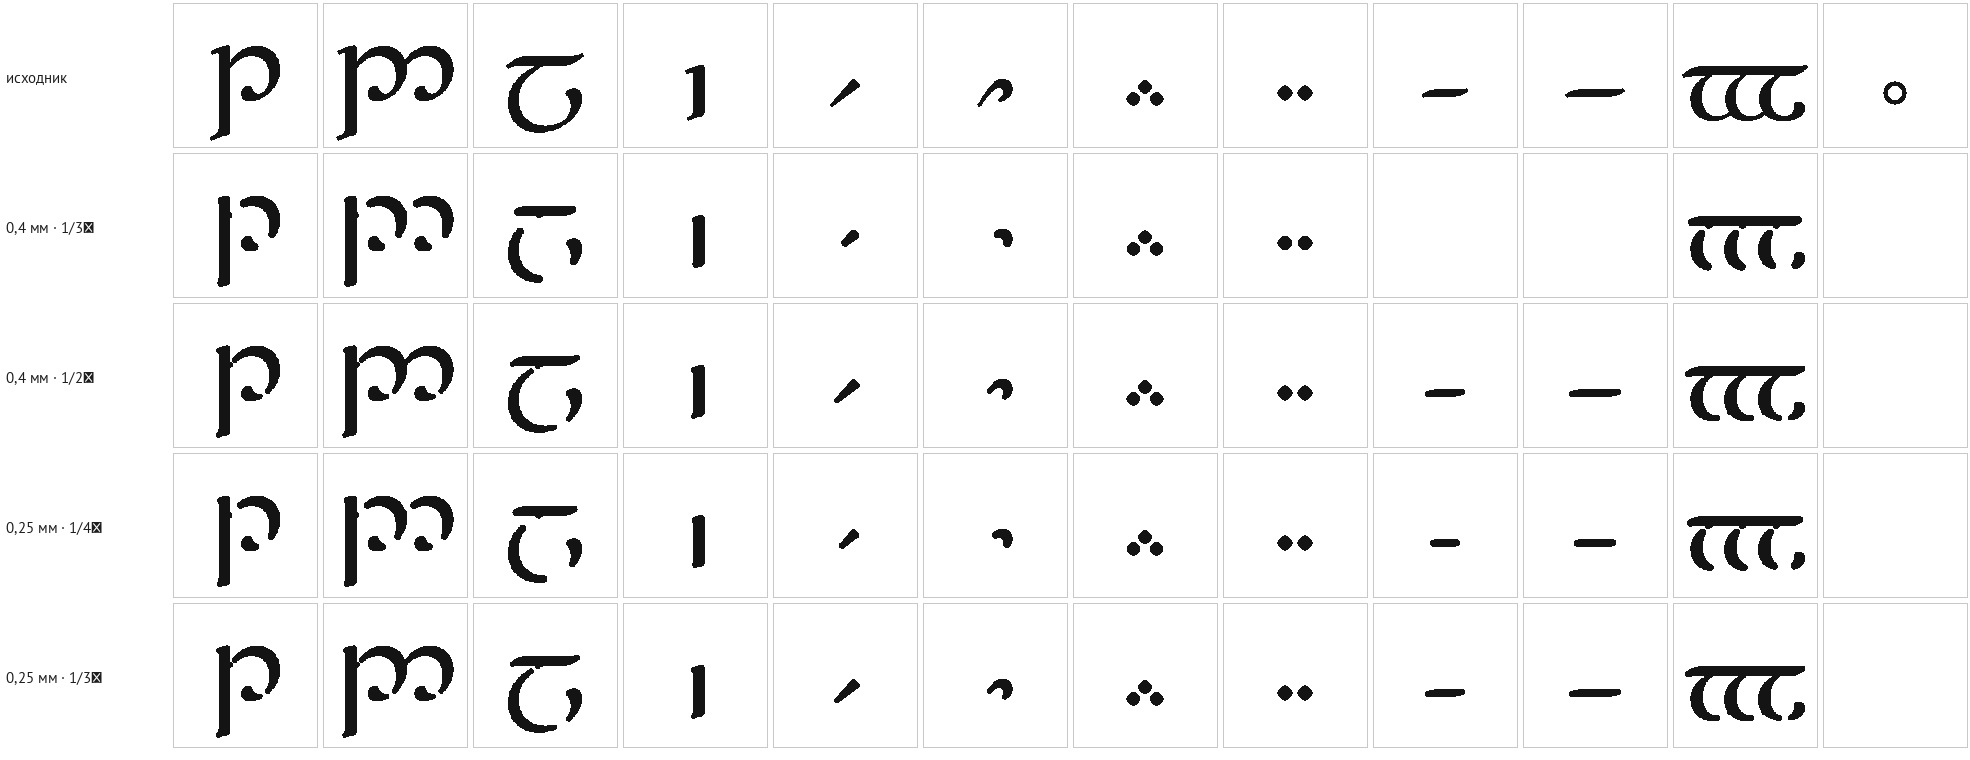
\includegraphics[width=\linewidth]{gen/fdm_panel.png}
\caption{Модель печати исходного рисунка Alcarin. Сверху — исходник; ниже — что останется после печати при разных соплах и кеглях.}
\label{fig:fdm1}
\end{figure}

\subsection{Наращивание тонких мест}

Рисунок Alcarin сохраняется, но каждая точка средней линии штриха получает не меньше минимальной толщины: к литере добавляется полоса шириной 0,45~мм (для сопла 0,25~мм — 0,30~мм) вдоль её средней линии. Толстые части остаются как были; утолщаются только волосяные соединения, острые концы и мелкие знаки. Литера при этом остаётся цельной — это один контур, а не сборка из элементов.

\begin{center}\small
\begin{tabular}{@{}lrrrrrrr@{}}
\toprule
& & \multicolumn{2}{c}{прирост, \%} & \multicolumn{2}{c}{потеря, \%} & & заплыв, \% \\
\cmidrule(lr){3-4}\cmidrule(lr){5-6}
сопло & em, мм & мед. & макс. & мед. & макс. & $n_{\text{пот}}$ & макс. \\
\midrule
\tabinput{gen/tab_fdmsim_thick.tex}
\bottomrule
\end{tabular}
\end{center}

\begin{figure}[H]
\centering
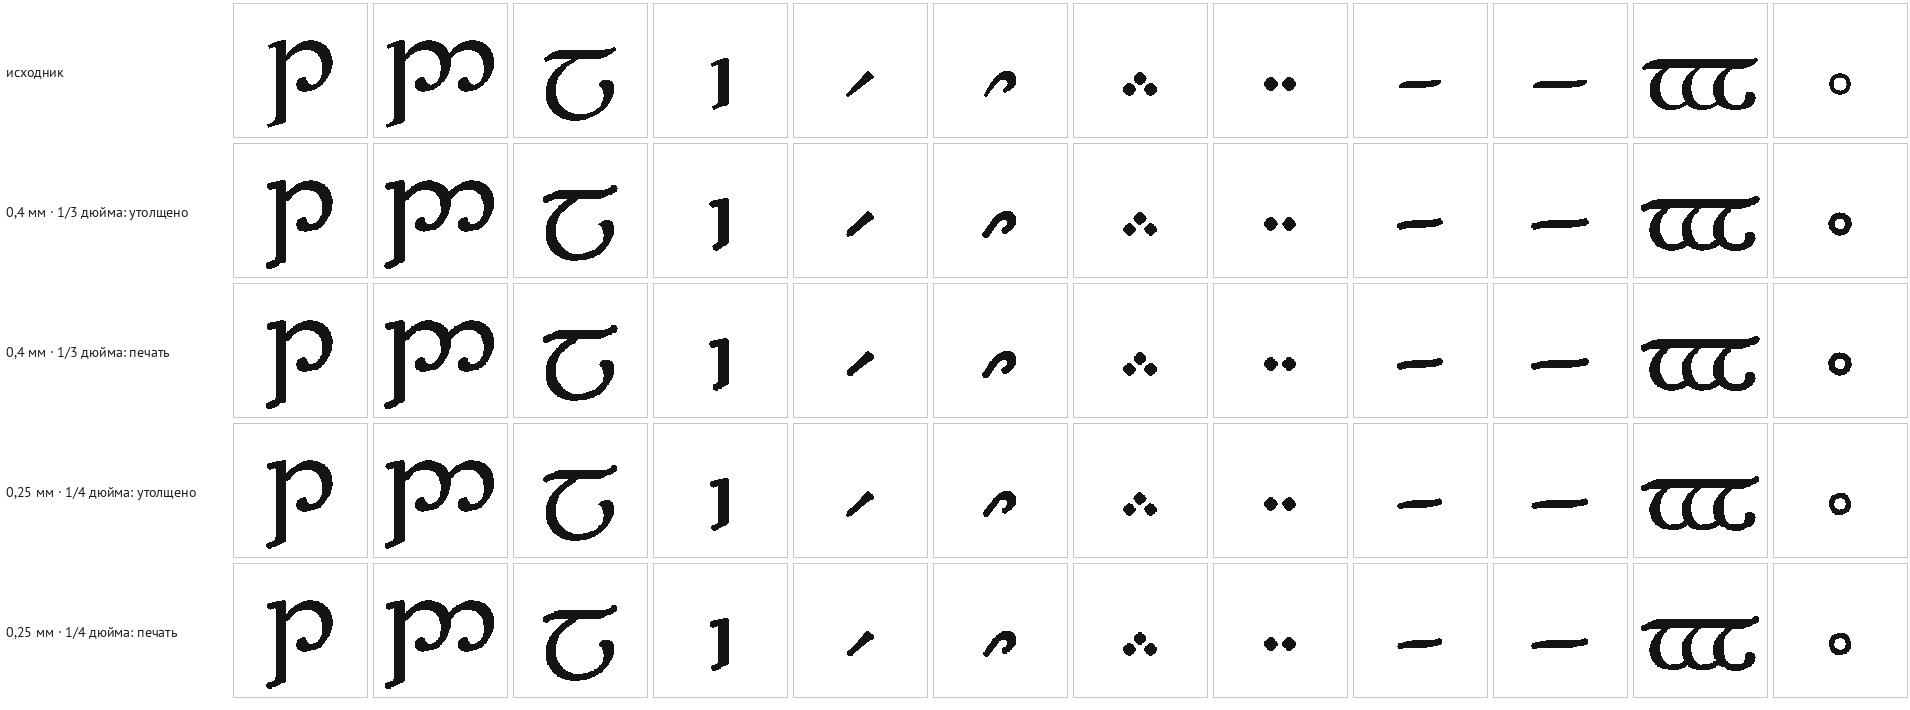
\includegraphics[width=\linewidth]{gen/fdm_panel2.png}
\caption{Наращивание и модель печати после него: литеры уцелели полностью.}
\label{fig:fdm2}
\end{figure}

\paragraph{Тонкие концы.} Скелет литеры у острого конца ветвится, и утолщение по такой развилке давало наплыв (в редакции 0.4 — на конце акута). Теперь каждая ветвь скелета перед утолщением укорачивается на радиус утолщения: развилки короче этого радиуса исчезают, а круг утолщения на новом конце доходит ровно туда, где кончалась ветвь. Точки-техты при этом не пропадают: от ветви, укороченной целиком, остаётся её середина. Наибольшее отклонение контура от рисунка у акута сократилось с 26 до 11 единиц шрифта (0,1~мм при 1/3''), у дуг — с 25 до 15--16.

\paragraph{Лицензия.} Alcarin распространяется по OFL 1.1 с зарезервированным именем «Alcarin». Изменённый рисунок можно использовать и распространять, но если он когда-нибудь будет оформлен как шрифт, его нельзя называть «Alcarin»; рабочее имя — «TPM Tengwar (на основе Alcarin Tengwar)». Метрики (ширины и оси) взяты из Alcarin без изменений.

%=====================================================================
\section{Общая схема}

\begin{figure}[h]
\centering
\begin{tikzpicture}[x=1mm,y=1mm]
\fill[gray!8] (0,70) rectangle (160,76);
\draw[thinmech] (0,70) -- (160,70) (0,76) -- (160,76);
\node[lbl] at (22,73) {лист на каретке};
\draw[arr] (150,80) -- node[lbl,above]{подача $w$} (125,80);
\draw[mech,fill=adv!60,rounded corners=1pt] (60,56) rectangle (100,62);
\node[lbl] at (80,59) {челнок};
\draw[mech] (62,56) -- (62,46) -- (98,46) -- (98,56);
\draw[mech] (98,46) -- (110,46) -- (110,86) -- (86,86);
\draw[mech,fill=gray!20] (80,84) rectangle (86,88); \node[lbl,anchor=south] at (83,88.5) {молоток};
\draw[arr] (83,84) -- (83,77);
\node[lbl,anchor=west,align=left] at (111,66) {U-образная\\рама};
\fill[axisred] (83,70) circle (0.9);
\draw[mech,fill=gray!12] (40,40) rectangle (130,44);
\node[lbl,anchor=north] at (85,39.5) {ползун: ход назад до 17\,u (9 мм), параллельно листу};
\draw[thinmech] (80,44) -- (80,46);
\draw[mech,fill=ink!70] (132,38) rectangle (135,48); \node[lbl,anchor=west,align=left] at (136,43) {нулевой\\упор};
\draw[mech,fill=sledA!60] (34,46) rectangle (37,50); \draw[mech,fill=sledB!60] (30,38) rectangle (33,42);
\node[lbl,anchor=east,text=sledA] at (29,50) {упор $b$};
\node[lbl,anchor=east,text=sledB] at (29,37) {упор $c$};
\draw[{Latex[length=1.6mm]}-,thick,draw=accent] (44,51) -- ++(14,0) node[lbl,right,text=accent]{отвод};
\draw[mech,fill=white,rounded corners=1pt] (2,6) rectangle (52,22);
\node[lbl,align=center] at (27,14) {сектора памяти B, C, W\\с фиксаторами и защёлками};
\draw[sledA,thick] (20,22) -- (35.5,46); \draw[sledB,thick] (30,22) -- (31.5,38);
\draw[mech,fill=white,rounded corners=1pt] (58,6) rectangle (110,22);
\node[lbl,align=center] at (84,14) {пластины признаков, планки\\R, W (пробелы), О, N; выбор};
\draw[mech,fill=sledA!25,rounded corners=1pt] (64,49) rectangle (96,54);
\node[lbl] at (80,51.5) {щупы W, B, C};
\draw[arr,dashed,sledA] (64,51.5) -- (40,51.5) -- (40,22);
\draw[arr,dashed,sledA] (96,51.5) -- (104,51.5) -- (104,34) -- (137,34) -- (137,22);
\node[lbl,anchor=south,text=sledA] at (122,34) {трос W};
\node[lbl,anchor=east,text=sledA] at (39,30) {тросы B, C};
\draw[mech,fill=white,rounded corners=1pt] (116,6) rectangle (158,22);
\node[lbl,align=center] at (137,14) {спуск: колесо, собачка,\\переставной упор $w$};
\draw[arr] (58,14) -- (52,14); \draw[arr] (110,14) -- (116,14);
\draw[thinmech] (150,22) -- (150,70);
\node[lbl,anchor=west,align=left] at (151,30) {к рейке\\каретки};
\draw[arr] (84,22) -- (84,40) node[pos=0.5,lbl,right]{О};
\end{tikzpicture}
\caption{ТПМ-2, вид сверху (условно). Челнок и молоток сидят на одной U-образной раме, рама — на ползуне. В покое ползун прижат пружиной к нулевому упору; для мёртвого знака планка О отводит его до упора $b$ или $c$, выбор делает признак N. Щупы на раме читают код литеры с кодовой гребёнки челнока и тросами ставят упор спуска и сектора B, C (ред. 0.10). Красная точка — ось молотка.}
\label{fig:top}
\end{figure}

\paragraph{Из чего состоит.} Остов по схеме Хаммонда (челнок на вертикальном валу, молоток, каретка с пружинным двигателем, колесо спуска), пружинный двигатель с цикловым валом, коромысла выбора позиции и ряда с фиксаторами, а также ползун с упорами, головка чтения кода с тремя щупами и тросами, пластины признаков, четыре мерные рамки (R, W, О, N), два ползунка B и C, переставной упор спуска с задвижкой, три сектора памяти и блокировки; на челноке — 11 литерных блоков и 11 кодовых гребёнок. Полный перечень — в \S\ref{sec:spec}.

%=====================================================================
\section{Видимость строки}
\label{sec:vis}
\begingroup\sloppy

\paragraph{Что было не так.} В редакции 0.7 челнок между ударами стоял в середине хода, между четвёртым и пятым рядами: его верхняя половина поднималась выше строки, а лента оставалась на линии печати. Глаз пишущего смотрит на лист сверху и спереди, примерно на 45° вниз, и челнок с лентой закрывали как раз то, что только что напечатано. Это проверено на модели: из глаза проводятся лучи к точкам листа, и точка считается закрытой, если на луче есть любая деталь машинки в покое. Три посадки: обычная (глаз в 720~мм перед линией печати и на 460~мм выше стола), выше и ближе (640 и 520~мм), ниже и дальше (780 и 400~мм). Считается полоса строки длиной 150~мм влево от точки печати (уже напечатанный текст), высота строки — 1,6~em.

\begin{center}\small
\begin{tabular}{@{}lcccccc@{}}
\toprule
& \multicolumn{3}{c}{ред. 0.7} & \multicolumn{3}{c}{ред. 0.8} \\
\cmidrule(lr){2-4}\cmidrule(lr){5-7}
посадка & текущая & предыдущая & третья выше & текущая & предыдущая & третья выше \\
\midrule
\tabinput{gen/tab_visibility.tex}
\bottomrule
\end{tabular}
\end{center}

\noindent{\small В каждой клетке — доля полосы 150~мм, которая закрыта, и сколько миллиметров строки от точки печати влево не видно совсем. Четвёртая строка и выше были видны и раньше.}

Впечатление верное: в редакции 0.7 последние \mvbefore~мм текущей строки (около 11~em, полтора-два десятка знаков) и последние \mvbeforeold~мм трёх предыдущих строк были закрыты челноком и лентой. Увидеть только что напечатанное можно было, лишь привстав или прокрутив лист.

\paragraph{Что сделано.}
\begin{enumerate}
  \item \textbf{Челнок в покое опущен под строку.} Исходное положение подъёма — на шаг ряда ниже верхнего ряда челнока (ряд $-1$): верхняя кромка челнока ниже строки. Чтобы при этом челнок не задел колесо фиксатора, линия печати поднята на 9~мм (до 234~мм над столом), а бобышка направляющего прутка опущена.
  \item \textbf{Лента отходит вниз.} Вибратор ленты — вилка из жести на ползуне под челноком — держит ленту на 10~мм ниже строки и поднимает её только на время удара своим кулачком. Так устроено большинство пишущих машинок с видимым письмом.
  \item \textbf{Ряды переставлены по частоте.} Теперь каждый знак сначала поднимает челнок из-под строки, и дальний ряд стал дальше. Чтобы средний путь не вырос, ближе к строке стоят частые ряды. Частоты оценены транскрипцией в режиме тэхт (\code{tools/model/freq.py}) на 164 именах и коротких фразах квенья и синдарина — 1089 ударов: основной ряд клавиатуры даёт 55\,\% ударов, верхний буквенный — 21\,\%, нижний — 19,5\,\%, верхний регистр — около 4\,\%, цифровой ряд — почти ничего. Основной ряд занимает верхний ряд челнока, цифровой — четвёртый; верхний регистр — ряды 5--8 в том же порядке.
\end{enumerate}

\paragraph{Чего это стоит.} Время оборота считалось для всех литер с весами частот (\S\ref{sec:motor}). Момент на цикловом валу вырос с \mtauold\ до \mtauC~мН$\cdot$м, энергия на знак — с \mEold\ до \mEchar~мДж, на \mavgcost\,\%; среднее время знака не изменилось (\mtavg~с), худшее — дальняя литера в нижнем, восьмом ряду челнока — выросло с \mtworstold\ до \mtworst~с, но такие знаки встречаются редко. Если только переставить ряды и оставить челнок в середине, нужно \mtauorder~мН$\cdot$м: частые ряды оказались бы дальше от исходного положения.

После переделки строки видны целиком при всех трёх посадках; при низкой посадке последние 6~мм текущей строки закрывает направляющий пруток каретки, остальное — доли процента у торца каретки.

\begin{figure}[H]
\centering
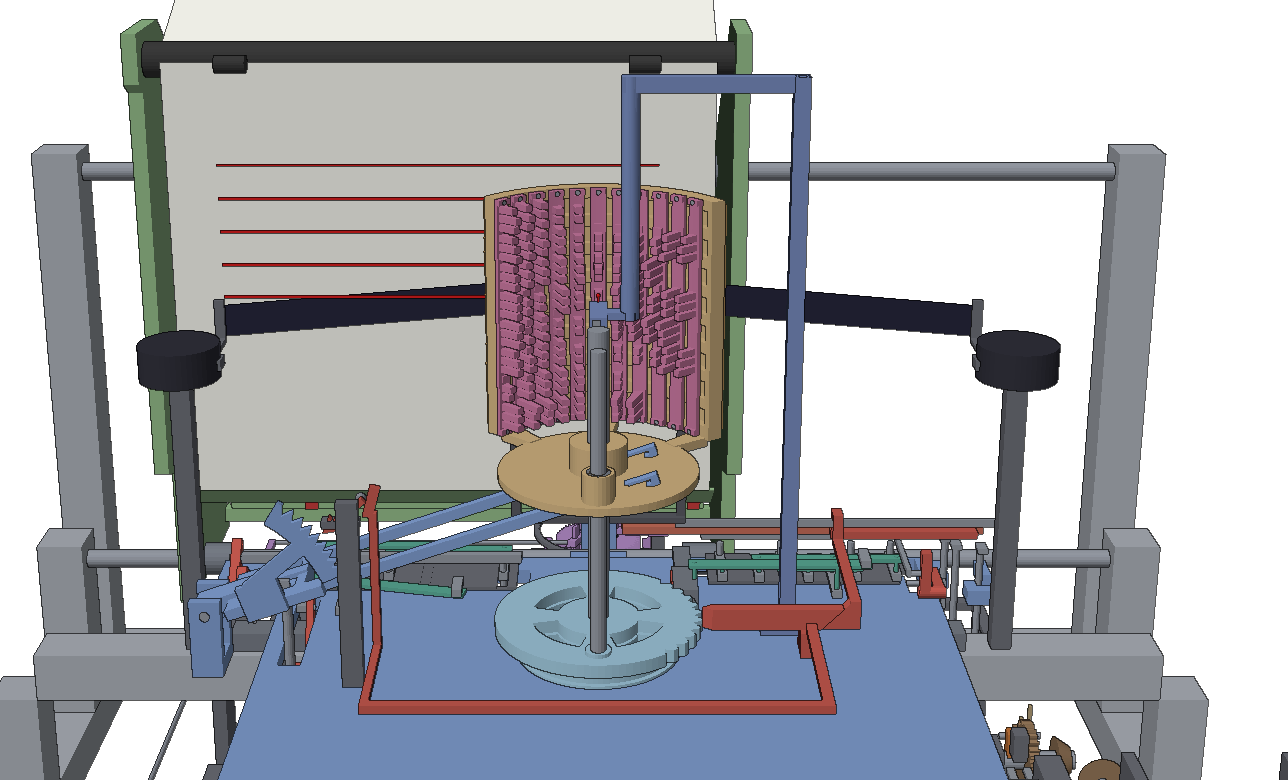
\includegraphics[width=0.49\linewidth]{gen/model/renders/view_before.png}\hfill
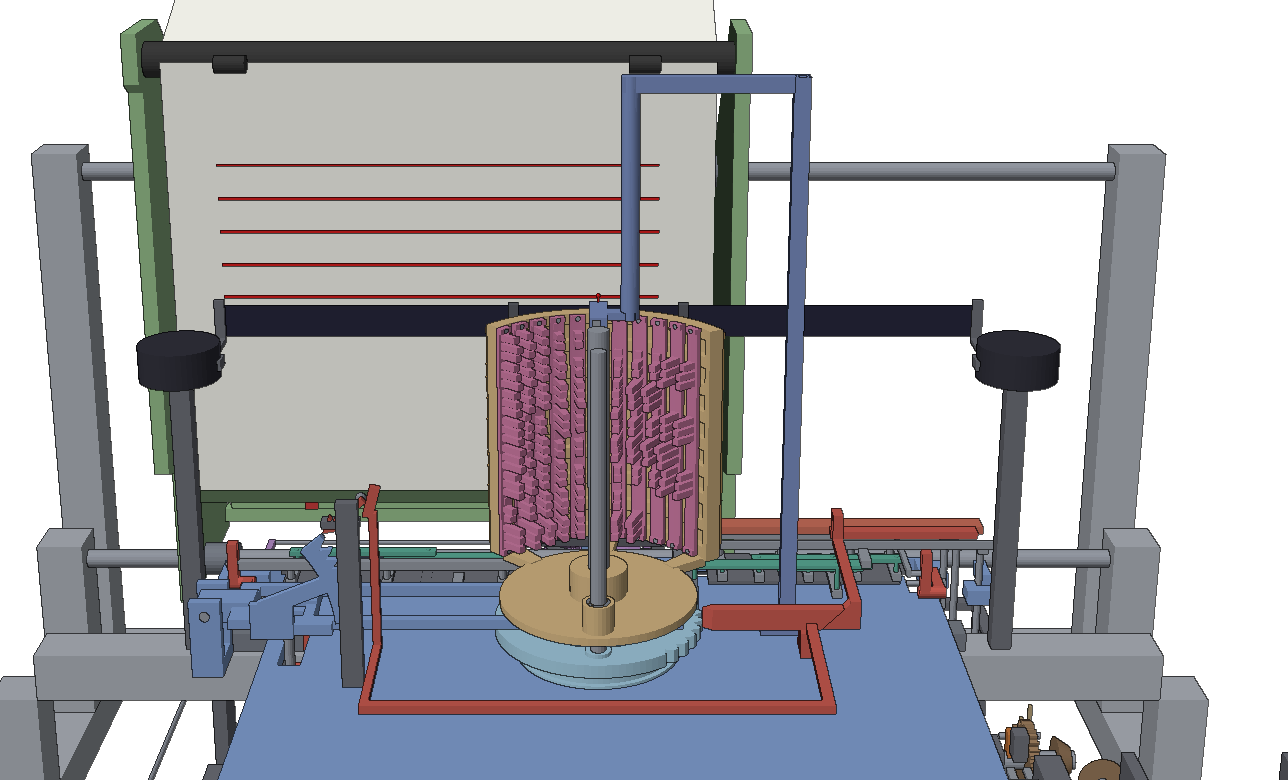
\includegraphics[width=0.49\linewidth]{gen/model/renders/view_after.png}
\caption{Вид с места пишущего (обычная посадка). Красные полосы — пять последних строк, текущая внизу. Слева — покой редакции 0.7: челнок в середине хода и лента на линии печати закрывают конец строк; справа — редакция 0.8: челнок под строкой, лента опущена.}
\label{fig:vis}
\end{figure}
\endgroup

%=====================================================================
\section{Узлы}

\subsection{Выбор позиции и ряда}
\label{sec:select}

Клавиша не двигает челнок сама: она только сообщает, куда его повернуть и на сколько поднять. Хвосты рычагов за осью поднимаются при нажатии. Над хвостами каждого столбца клавиатуры лежит толкатель; он поднимает планки разрядов позиции — четыре планки r1, r2, r4, r8, по двоичной записи номера столбца (выступ толкателя есть только под планками, чьи разряды равны единице). Выше лежат три планки ряда: l1 (выступы на рычагах первого и второго рядов клавиатуры), l2 (первого и четвёртого) и l4 (клавиша регистра). Ряды клавиатуры занимают ряды челнока по частоте (\S\ref{sec:vis}): основной ряд — код 0, верхний буквенный — 1, нижний — 2, цифровой — 3; верхний регистр — те же коды плюс 4. Поднятая планка через стержень ставит защёлку на своём коромысле.

\paragraph{Коромысла.} На плите печатающего узла стоят два набора коромысел (whiffletree, как в машинках с шаровой головкой): поворота (четыре разряда) и подъёма (три разряда). В начале цикла кулачок толкает приводную планку; разряды с поставленной защёлкой проходят свой полный ход, остальные стоят. Коромысла складывают ходы с весами 1, 2, 4, 8 и вычитают постоянное смещение; устройство звеньев — в \S\ref{sec:links}. Выход поворота — каретка на короткой направляющей MGN7, к которой пристёгнута стальная лента 5$\times$0,1~мм; лента навита на шкив радиусом 30~мм на валу челнока и поворачивает его на 9,6° (5,0~мм ленты) на позицию. Выход подъёма — вилка под ступицей челнока: 11,43~мм на ряд.

\paragraph{Фиксаторы.} Коромысла дают положение с точностью нескольких десятых миллиметра; точное положение даёт фиксатор. На валу под челноком сидит колесо радиусом 40~мм с 11 клиновыми вырезами; в конце хода кулачок вводит в вырез стальной клин, и колесо доворачивается на место. Так же фиксируется ряд — клином в гребёнке на вилке подъёма. Лента и коромысла рассчитаны на то, чтобы уступить фиксатору половину шага.

\paragraph{Расчёт коромысел.}
\label{sec:whiffle}
Разряд с поставленной защёлкой проходит $S = 12$~мм. Каждое коромысло складывает уже набранную сумму с очередным разрядом, и узел делит рычаг в отношении весов. На выходе дерева код $c$ даёт $c \cdot S/15$ (для подъёма $S/7$); выходной рычаг увеличивает это в \mgrot\ раза для поворота (5,03~мм ленты на позицию) и в \mglift\ раза для подъёма (11,43~мм на ряд; рычаг 1,33 и вилка 1:5). Постоянное смещение задаёт опора выходного рычага, сдвигаемая той же приводной планкой. Размеры коромысел — в таблице на с.~\pageref{tab:ladder}.

\sloppy Ошибки коромысел: разброс хода кулачка и защёлок (0,05~мм), смещение отверстий (0,05~мм), люфт в каждом шарнире ($\pm0{,}05$~мм, стальные оси в развёрнутых отверстиях), ошибка передаточного числа выходного рычага (0,5\,\%) и смещения. Монте-Карло по 8000 машинок; для каждой берётся наихудшая из 11 позиций (8 рядов). Захват фиксатора — почти полшага: \mbox{$\pm$\mcaprot~мм} ленты для поворота и \mbox{$\pm$\mcaplift~мм} для подъёма.

\begin{center}\small
\begin{tabularx}{\linewidth}{@{}rXrrrrr@{}}
\toprule
& & & \multicolumn{2}{c}{поворот, мм} & \multicolumn{2}{c}{подъём, мм} \\
\cmidrule(lr){4-5}\cmidrule(lr){6-7}
$S$, мм & вариант & усиление & 95\,\% & 99,7\,\% & 95\,\% & 99,7\,\% \\
\midrule
\tabinput{gen/tab_whiffle.tex}
\bottomrule
\end{tabularx}
\end{center}

\noindent{\small «После настройки» — передаточное число и нуль выставлены регулировочными винтами по контрольному набору; остаются люфты и разброс ходов.}

При ходе разряда 6~мм ошибка поворота доходила до 2,1~мм при захвате 2,4~мм, а при вдвое худших допусках фиксатор промахивался бы на каждой девятой машинке. При 12~мм наихудшая ошибка — около 1~мм, то есть меньше половины захвата даже при вдвое худших допусках. Поэтому кулачки поворота и подъёма дают ход 12~мм, а вырезы колеса фиксатора сделаны почти во весь шаг (V-образные, раствор 6,3~мм на радиусе 41~мм; клин собачки повторяет их профиль).

\begin{figure}[H]
\centering
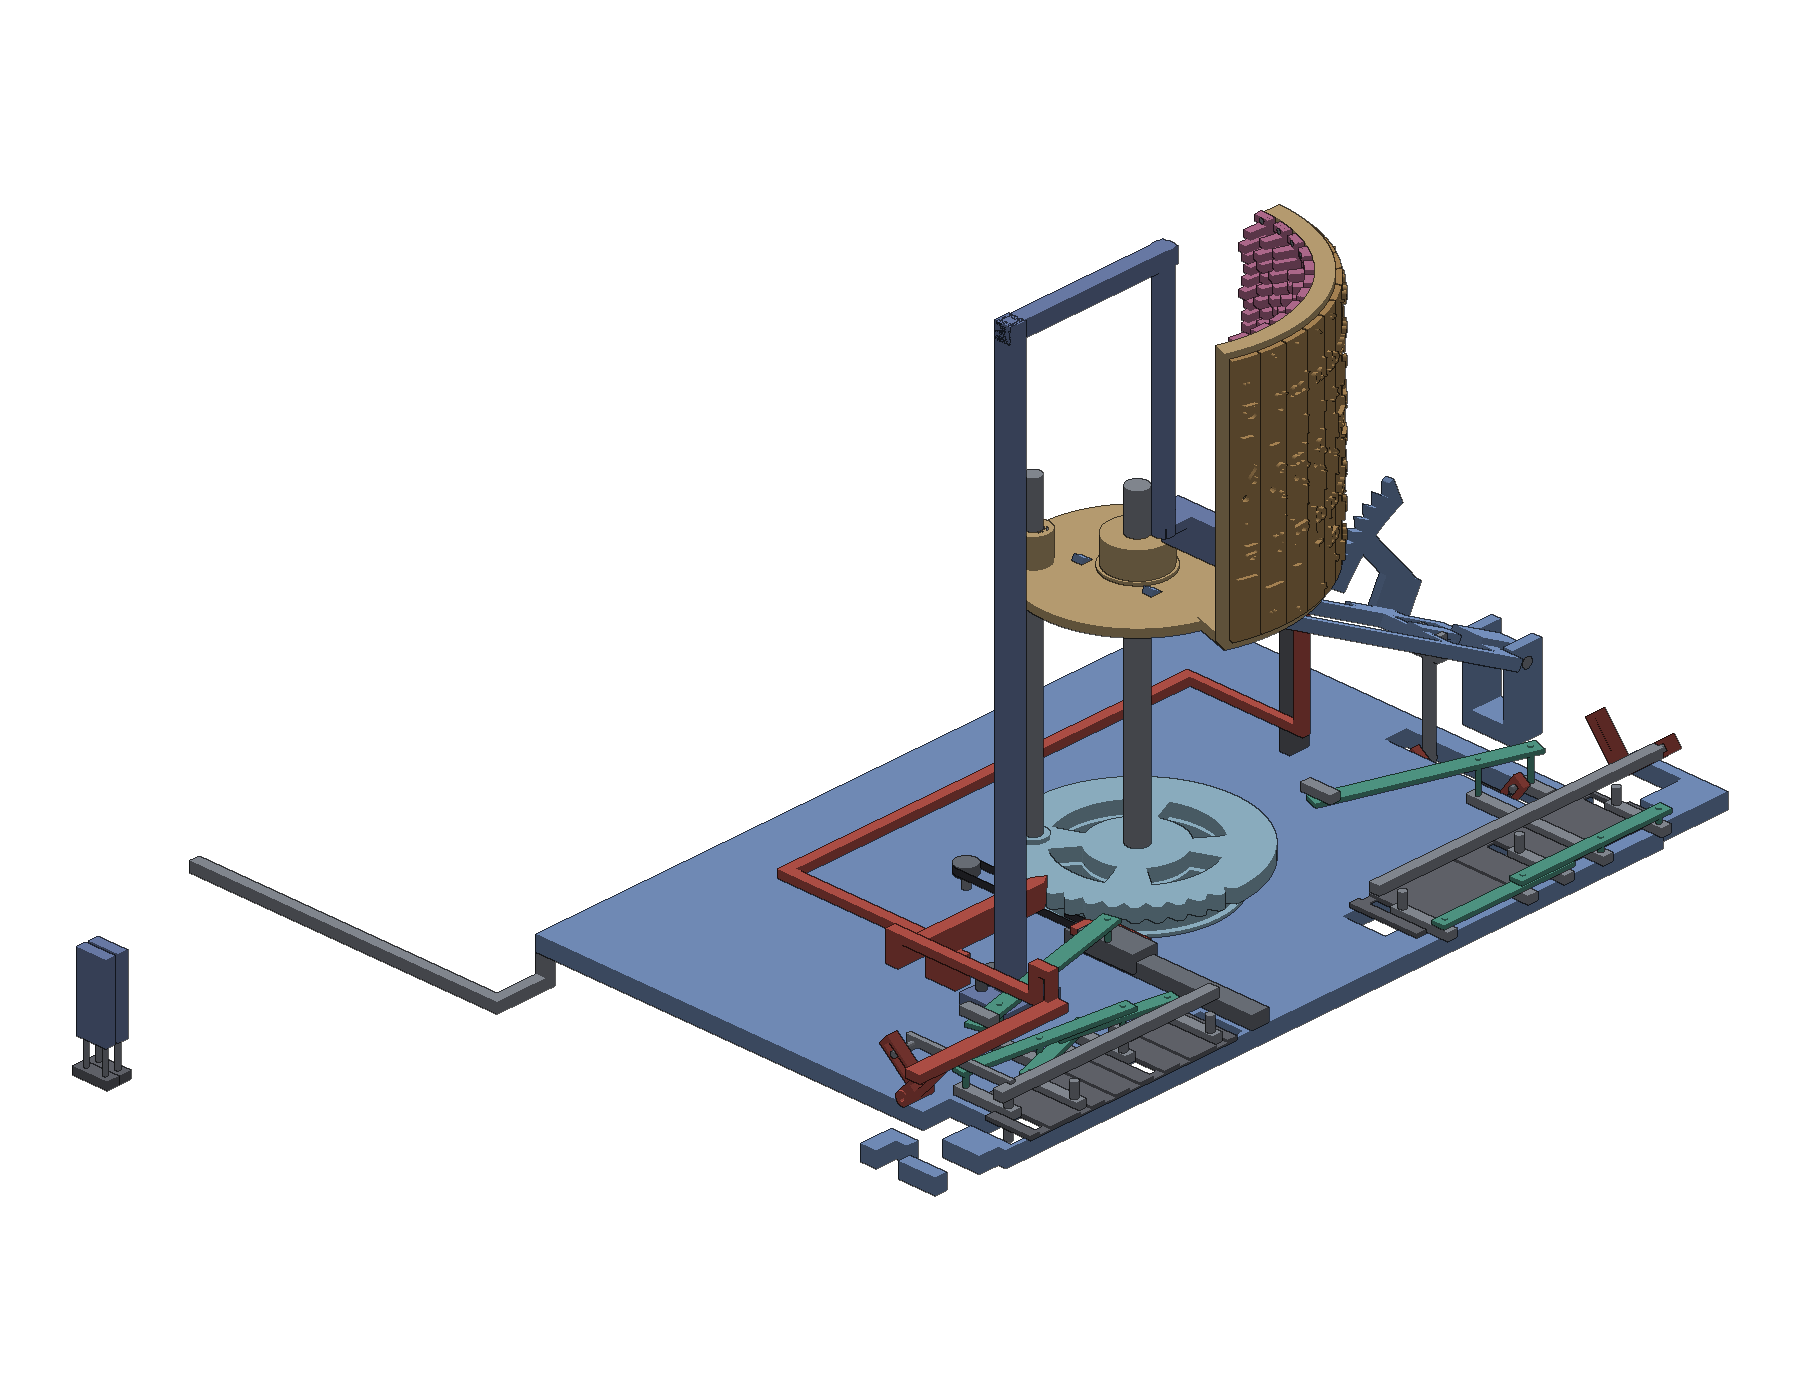
\includegraphics[width=0.82\linewidth]{gen/model/renders/print_unit.png}
\caption{Печатающий узел в модели (челнок на позиции 10, в ряду 7). На плите: коромысла поворота и подъёма с приводными планками; выход поворота — каретка с лентой, навитой на шкив под челноком; колесо фиксатора над шкивом и клин фиксатора (красный); вилка подъёма с гребёнкой фиксатора ряда.}
\label{fig:pins}
\end{figure}

\paragraph{Развёртка челнока.} Расположение литер по рядам и позициям — на рис.~\ref{fig:shuttle}. Каждая позиция — литерный блок на 8 литер. Продвигающая литера отлита так, что против оси молотка встаёт левый край её клетки; мёртвый знак — так, что его якорь стоит на 8\,u правее оси.

\begin{figure}[h]
\centering
\setlength\tgem{9.5mm}
\begin{tikzpicture}[x=\tgu,y=\tgu]
\node[lbl,anchor=east] at (-150,200) {1};
\draw[slug,fill=white] (0.0,-380) rectangle (1147.5,780);
\fill[cellfill] (62.5,-330) rectangle (687.5,740);
\node[anchor=base west,inner sep=0pt,outer sep=0pt] at (82.5,0.0) {\TG{62}};
\draw[ppoint,thin] (62.5,-380) -- (62.5,780);
\draw[slug,fill=white] (1187.5,-380) rectangle (2335.0,780);
\fill[cellfill] (1250.0,-330) rectangle (1875.0,740);
\node[anchor=base west,inner sep=0pt,outer sep=0pt] at (1262.0,0.0) {\TG{63}};
\draw[ppoint,thin] (1250.0,-380) -- (1250.0,780);
\draw[slug,fill=white] (2375.0,-380) rectangle (3522.5,780);
\fill[cellfill] (2437.5,-330) rectangle (3062.5,740);
\node[anchor=base west,inner sep=0pt,outer sep=0pt] at (2454.5,0.0) {\TG{64}};
\draw[ppoint,thin] (2437.5,-380) -- (2437.5,780);
\draw[slug,fill=white] (3562.5,-380) rectangle (4710.0,780);
\fill[cellfill] (3625.0,-330) rectangle (4625.0,740);
\node[anchor=base west,inner sep=0pt,outer sep=0pt] at (3645.0,0.0) {\TG{70}};
\draw[ppoint,thin] (3625.0,-380) -- (3625.0,780);
\draw[slug,fill=white] (4750.0,-380) rectangle (5897.5,780);
\fill[cellfill] (4812.5,-330) rectangle (5812.5,740);
\node[anchor=base west,inner sep=0pt,outer sep=0pt] at (4824.5,0.0) {\TG{71}};
\draw[ppoint,thin] (4812.5,-380) -- (4812.5,780);
\draw[slug,fill=white] (5937.5,-380) rectangle (7085.0,780);
\fill[sledA!12] (5937.5,-380) rectangle (7085.0,780);
\node[anchor=base west,inner sep=0pt,outer sep=0pt] at (6423.0,0.0) {\TG{315}};
\draw[ppoint,thin] (6000.0,-380) -- (6000.0,780);
\draw[slug,fill=white] (7125.0,-380) rectangle (8272.5,780);
\fill[sledA!12] (7125.0,-380) rectangle (8272.5,780);
\node[anchor=base west,inner sep=0pt,outer sep=0pt] at (7528.5,0.0) {\TG{311}};
\draw[ppoint,thin] (7187.5,-380) -- (7187.5,780);
\draw[slug,fill=white] (8312.5,-380) rectangle (9460.0,780);
\fill[sledA!12] (8312.5,-380) rectangle (9460.0,780);
\node[anchor=base west,inner sep=0pt,outer sep=0pt] at (8762.0,0.0) {\TG{317}};
\draw[ppoint,thin] (8375.0,-380) -- (8375.0,780);
\draw[slug,fill=white] (9500.0,-380) rectangle (10647.5,780);
\fill[sledA!12] (9500.0,-380) rectangle (10647.5,780);
\node[anchor=base west,inner sep=0pt,outer sep=0pt] at (9937.5,0.0) {\TG{321}};
\draw[ppoint,thin] (9562.5,-380) -- (9562.5,780);
\draw[slug,fill=white] (10687.5,-380) rectangle (11835.0,780);
\fill[sledA!12] (10687.5,-380) rectangle (11835.0,780);
\node[anchor=base west,inner sep=0pt,outer sep=0pt] at (11128.0,0.0) {\TG{324}};
\draw[ppoint,thin] (10750.0,-380) -- (10750.0,780);
\draw[slug,fill=white] (11875.0,-380) rectangle (13022.5,780);
\fill[sledB!12] (11875.0,-380) rectangle (13022.5,780);
\node[anchor=base west,inner sep=0pt,outer sep=0pt] at (12285.5,0.0) {\TG{314}};
\draw[ppoint,thin] (11937.5,-380) -- (11937.5,780);
\node[lbl,anchor=east] at (-150,-1550) {2};
\draw[slug,fill=white] (0.0,-2130) rectangle (1147.5,-970);
\fill[cellfill] (62.5,-2080) rectangle (687.5,-1010);
\node[anchor=base west,inner sep=0pt,outer sep=0pt] at (72.0,-1750.0) {\TG{54}};
\draw[ppoint,thin] (62.5,-2130) -- (62.5,-970);
\draw[slug,fill=white] (1187.5,-2130) rectangle (2335.0,-970);
\fill[cellfill] (1250.0,-2080) rectangle (1875.0,-1010);
\node[anchor=base west,inner sep=0pt,outer sep=0pt] at (1251.5,-1750.0) {\TG{55}};
\draw[ppoint,thin] (1250.0,-2130) -- (1250.0,-970);
\draw[slug,fill=white] (2375.0,-2130) rectangle (3522.5,-970);
\fill[cellfill] (2437.5,-2080) rectangle (3062.5,-1010);
\node[anchor=base west,inner sep=0pt,outer sep=0pt] at (2447.0,-1750.0) {\TG{56}};
\draw[ppoint,thin] (2437.5,-2130) -- (2437.5,-970);
\draw[slug,fill=white] (3562.5,-2130) rectangle (4710.0,-970);
\fill[cellfill] (3625.0,-2080) rectangle (4250.0,-1010);
\node[anchor=base west,inner sep=0pt,outer sep=0pt] at (3614.5,-1750.0) {\TG{57}};
\draw[ppoint,thin] (3625.0,-2130) -- (3625.0,-970);
\draw[slug,fill=white] (4750.0,-2130) rectangle (5897.5,-970);
\fill[cellfill] (4812.5,-2080) rectangle (5812.5,-1010);
\node[anchor=base west,inner sep=0pt,outer sep=0pt] at (4830.5,-1750.0) {\TG{58}};
\draw[ppoint,thin] (4812.5,-2130) -- (4812.5,-970);
\draw[slug,fill=white] (5937.5,-2130) rectangle (7085.0,-970);
\fill[cellfill] (6000.0,-2080) rectangle (7000.0,-1010);
\node[anchor=base west,inner sep=0pt,outer sep=0pt] at (6009.0,-1750.0) {\TG{59}};
\draw[ppoint,thin] (6000.0,-2130) -- (6000.0,-970);
\draw[slug,fill=white] (7125.0,-2130) rectangle (8272.5,-970);
\fill[cellfill] (7187.5,-2080) rectangle (8125.0,-1010);
\node[anchor=base west,inner sep=0pt,outer sep=0pt] at (7183.0,-1750.0) {\TG{68}};
\draw[ppoint,thin] (7187.5,-2130) -- (7187.5,-970);
\draw[slug,fill=white] (8312.5,-2130) rectangle (9460.0,-970);
\fill[cellfill] (8375.0,-2080) rectangle (9312.5,-1010);
\node[anchor=base west,inner sep=0pt,outer sep=0pt] at (8351.0,-1750.0) {\TG{66}};
\draw[ppoint,thin] (8375.0,-2130) -- (8375.0,-970);
\draw[slug,fill=white] (9500.0,-2130) rectangle (10647.5,-970);
\fill[cellfill] (9562.5,-2080) rectangle (10500.0,-1010);
\node[anchor=base west,inner sep=0pt,outer sep=0pt] at (9539.5,-1750.0) {\TG{67}};
\draw[ppoint,thin] (9562.5,-2130) -- (9562.5,-970);
\draw[slug,fill=white] (10687.5,-2130) rectangle (11835.0,-970);
\fill[cellfill] (10750.0,-2080) rectangle (11250.0,-1010);
\node[anchor=base west,inner sep=0pt,outer sep=0pt] at (10746.0,-1750.0) {\TG{86}};
\draw[ppoint,thin] (10750.0,-2130) -- (10750.0,-970);
\draw[slug,fill=white] (11875.0,-2130) rectangle (13022.5,-970);
\fill[cellfill] (11937.5,-2080) rectangle (12625.0,-1010);
\node[anchor=base west,inner sep=0pt,outer sep=0pt] at (11959.5,-1750.0) {\TG{88}};
\draw[ppoint,thin] (11937.5,-2130) -- (11937.5,-970);
\node[lbl,anchor=east] at (-150,-3300) {3};
\draw[slug,fill=white] (0.0,-3880) rectangle (1147.5,-2720);
\fill[cellfill] (62.5,-3830) rectangle (687.5,-2760);
\node[anchor=base west,inner sep=0pt,outer sep=0pt] at (75.0,-3500.0) {\TG{74}};
\draw[ppoint,thin] (62.5,-3880) -- (62.5,-2720);
\draw[slug,fill=white] (1187.5,-3880) rectangle (2335.0,-2720);
\fill[cellfill] (1250.0,-3830) rectangle (1875.0,-2760);
\node[anchor=base west,inner sep=0pt,outer sep=0pt] at (1257.5,-3500.0) {\TG{75}};
\draw[ppoint,thin] (1250.0,-3880) -- (1250.0,-2720);
\draw[slug,fill=white] (2375.0,-3880) rectangle (3522.5,-2720);
\fill[cellfill] (2437.5,-3830) rectangle (3062.5,-2760);
\node[anchor=base west,inner sep=0pt,outer sep=0pt] at (2440.0,-3500.0) {\TG{76}};
\draw[ppoint,thin] (2437.5,-3880) -- (2437.5,-2720);
\draw[slug,fill=white] (3562.5,-3880) rectangle (4710.0,-2720);
\fill[cellfill] (3625.0,-3830) rectangle (4125.0,-2760);
\node[anchor=base west,inner sep=0pt,outer sep=0pt] at (3608.5,-3500.0) {\TG{90}};
\draw[ppoint,thin] (3625.0,-3880) -- (3625.0,-2720);
\draw[slug,fill=white] (4750.0,-3880) rectangle (5897.5,-2720);
\fill[cellfill] (4812.5,-3830) rectangle (5312.5,-2760);
\node[anchor=base west,inner sep=0pt,outer sep=0pt] at (4798.5,-3500.0) {\TG{91}};
\draw[ppoint,thin] (4812.5,-3880) -- (4812.5,-2720);
\draw[slug,fill=white] (5937.5,-3880) rectangle (7085.0,-2720);
\fill[cellfill] (6000.0,-3830) rectangle (6562.5,-2760);
\node[anchor=base west,inner sep=0pt,outer sep=0pt] at (5985.5,-3500.0) {\TG{94}};
\draw[ppoint,thin] (6000.0,-3880) -- (6000.0,-2720);
\draw[slug,fill=white] (7125.0,-3880) rectangle (8272.5,-2720);
\fill[cellfill] (7187.5,-3830) rectangle (7750.0,-2760);
\node[anchor=base west,inner sep=0pt,outer sep=0pt] at (7218.0,-3500.0) {\TG{96}};
\draw[ppoint,thin] (7187.5,-3880) -- (7187.5,-2720);
\draw[slug,fill=white] (8312.5,-3880) rectangle (9460.0,-2720);
\fill[cellfill] (8375.0,-3830) rectangle (8625.0,-2760);
\node[anchor=base west,inner sep=0pt,outer sep=0pt] at (8375.0,-3500.0) {\TG{100}};
\draw[ppoint,thin] (8375.0,-3880) -- (8375.0,-2720);
\draw[slug,fill=white] (9500.0,-3880) rectangle (10647.5,-2720);
\fill[cellfill] (9562.5,-3830) rectangle (9812.5,-2760);
\node[anchor=base west,inner sep=0pt,outer sep=0pt] at (9559.5,-3500.0) {\TG{98}};
\draw[ppoint,thin] (9562.5,-3880) -- (9562.5,-2720);
\draw[slug,fill=white] (10687.5,-3880) rectangle (11835.0,-2720);
\fill[sledB!12] (10687.5,-3880) rectangle (11835.0,-2720);
\node[anchor=base west,inner sep=0pt,outer sep=0pt] at (11006.0,-3500.0) {\TG{329}};
\draw[ppoint,thin] (10750.0,-3880) -- (10750.0,-2720);
\draw[slug,fill=white] (11875.0,-3880) rectangle (13022.5,-2720);
\fill[sledA!12] (11875.0,-3880) rectangle (13022.5,-2720);
\node[anchor=base west,inner sep=0pt,outer sep=0pt] at (12193.5,-3500.0) {\TG{328}};
\draw[ppoint,thin] (11937.5,-3880) -- (11937.5,-2720);
\node[lbl,anchor=east] at (-150,-5050) {4};
\draw[slug,fill=white] (0.0,-5630) rectangle (1147.5,-4470);
\fill[cellfill] (62.5,-5580) rectangle (562.5,-4510);
\node[anchor=base west,inner sep=0pt,outer sep=0pt] at (73.5,-5250.0) {\TG{195}};
\draw[ppoint,thin] (62.5,-5630) -- (62.5,-4470);
\draw[slug,fill=white] (1187.5,-5630) rectangle (2335.0,-4470);
\fill[cellfill] (1250.0,-5580) rectangle (2000.0,-4510);
\node[anchor=base west,inner sep=0pt,outer sep=0pt] at (1250.0,-5250.0) {\TG{196}};
\draw[ppoint,thin] (1250.0,-5630) -- (1250.0,-4470);
\draw[slug,fill=white] (2375.0,-5630) rectangle (3522.5,-4470);
\fill[cellfill] (2437.5,-5580) rectangle (3437.5,-4510);
\node[anchor=base west,inner sep=0pt,outer sep=0pt] at (2430.5,-5250.0) {\TG{197}};
\draw[ppoint,thin] (2437.5,-5630) -- (2437.5,-4470);
\draw[slug,fill=white] (3562.5,-5630) rectangle (4710.0,-4470);
\fill[cellfill] (3625.0,-5580) rectangle (3937.5,-4510);
\node[anchor=base west,inner sep=0pt,outer sep=0pt] at (3597.0,-5250.0) {\TG{198}};
\draw[ppoint,thin] (3625.0,-5630) -- (3625.0,-4470);
\draw[slug,fill=white] (4750.0,-5630) rectangle (5897.5,-4470);
\fill[cellfill] (4812.5,-5580) rectangle (5500.0,-4510);
\node[anchor=base west,inner sep=0pt,outer sep=0pt] at (4808.5,-5250.0) {\TG{199}};
\draw[ppoint,thin] (4812.5,-5630) -- (4812.5,-4470);
\draw[slug,fill=white] (5937.5,-5630) rectangle (7085.0,-4470);
\fill[cellfill] (6000.0,-5580) rectangle (6937.5,-4510);
\node[anchor=base west,inner sep=0pt,outer sep=0pt] at (5996.0,-5250.0) {\TG{200}};
\draw[ppoint,thin] (6000.0,-5630) -- (6000.0,-4470);
\draw[slug,fill=white] (7125.0,-5630) rectangle (8272.5,-4470);
\fill[cellfill] (7187.5,-5580) rectangle (7500.0,-4510);
\node[anchor=base west,inner sep=0pt,outer sep=0pt] at (7204.0,-5250.0) {\TG{201}};
\draw[ppoint,thin] (7187.5,-5630) -- (7187.5,-4470);
\draw[slug,fill=white] (8312.5,-5630) rectangle (9460.0,-4470);
\fill[cellfill] (8375.0,-5580) rectangle (9000.0,-4510);
\node[anchor=base west,inner sep=0pt,outer sep=0pt] at (8398.5,-5250.0) {\TG{202}};
\draw[ppoint,thin] (8375.0,-5630) -- (8375.0,-4470);
\draw[slug,fill=white] (9500.0,-5630) rectangle (10647.5,-4470);
\fill[cellfill] (9562.5,-5580) rectangle (10437.5,-4510);
\node[anchor=base west,inner sep=0pt,outer sep=0pt] at (9581.0,-5250.0) {\TG{203}};
\draw[ppoint,thin] (9562.5,-5630) -- (9562.5,-4470);
\draw[slug,fill=white] (10687.5,-5630) rectangle (11835.0,-4470);
\fill[cellfill] (10750.0,-5580) rectangle (11250.0,-4510);
\node[anchor=base west,inner sep=0pt,outer sep=0pt] at (10760.0,-5250.0) {\TG{194}};
\draw[ppoint,thin] (10750.0,-5630) -- (10750.0,-4470);
\draw[slug,fill=white] (11875.0,-5630) rectangle (13022.5,-4470);
\fill[cellfill] (11937.5,-5580) rectangle (12437.5,-4510);
\node[anchor=base west,inner sep=0pt,outer sep=0pt] at (11943.5,-5250.0) {\TG{204}};
\draw[ppoint,thin] (11937.5,-5630) -- (11937.5,-4470);
\node[lbl,anchor=east] at (-150,-6800) {5};
\draw[slug,fill=white] (0.0,-7380) rectangle (1147.5,-6220);
\fill[cellfill] (62.5,-7330) rectangle (500.0,-6260);
\node[anchor=base west,inner sep=0pt,outer sep=0pt] at (62.0,-7000.0) {\TG{92}};
\draw[ppoint,thin] (62.5,-7380) -- (62.5,-6220);
\draw[slug,fill=white] (1187.5,-7380) rectangle (2335.0,-6220);
\fill[cellfill] (1250.0,-7330) rectangle (1875.0,-6260);
\node[anchor=base west,inner sep=0pt,outer sep=0pt] at (1229.5,-7000.0) {\TG{95}};
\draw[ppoint,thin] (1250.0,-7380) -- (1250.0,-6220);
\draw[slug,fill=white] (2375.0,-7380) rectangle (3522.5,-6220);
\fill[cellfill] (2437.5,-7330) rectangle (3062.5,-6260);
\node[anchor=base west,inner sep=0pt,outer sep=0pt] at (2434.5,-7000.0) {\TG{65}};
\draw[ppoint,thin] (2437.5,-7380) -- (2437.5,-6220);
\draw[slug,fill=white] (3562.5,-7380) rectangle (4710.0,-6220);
\fill[cellfill] (3625.0,-7330) rectangle (4625.0,-6260);
\node[anchor=base west,inner sep=0pt,outer sep=0pt] at (3635.0,-7000.0) {\TG{72}};
\draw[ppoint,thin] (3625.0,-7380) -- (3625.0,-6220);
\draw[slug,fill=white] (4750.0,-7380) rectangle (5897.5,-6220);
\fill[cellfill] (4812.5,-7330) rectangle (5812.5,-6260);
\node[anchor=base west,inner sep=0pt,outer sep=0pt] at (4802.5,-7000.0) {\TG{73}};
\draw[ppoint,thin] (4812.5,-7380) -- (4812.5,-6220);
\draw[slug,fill=white] (5937.5,-7380) rectangle (7085.0,-6220);
\fill[cellfill] (6000.0,-7330) rectangle (6250.0,-6260);
\node[anchor=base west,inner sep=0pt,outer sep=0pt] at (5997.0,-7000.0) {\TG{98}};
\node[anchor=base west,inner sep=0pt,outer sep=0pt] at (6048.0,-7000.0) {\TG{315}};
\draw[ppoint,thin] (6000.0,-7380) -- (6000.0,-6220);
\draw[slug,fill=white] (7125.0,-7380) rectangle (8272.5,-6220);
\fill[cellfill] (7187.5,-7330) rectangle (7437.5,-6260);
\node[anchor=base west,inner sep=0pt,outer sep=0pt] at (7184.5,-7000.0) {\TG{98}};
\node[anchor=base west,inner sep=0pt,outer sep=0pt] at (7153.5,-7000.0) {\TG{311}};
\draw[ppoint,thin] (7187.5,-7380) -- (7187.5,-6220);
\draw[slug,fill=white] (8312.5,-7380) rectangle (9460.0,-6220);
\fill[cellfill] (8375.0,-7330) rectangle (8625.0,-6260);
\node[anchor=base west,inner sep=0pt,outer sep=0pt] at (8372.0,-7000.0) {\TG{98}};
\node[anchor=base west,inner sep=0pt,outer sep=0pt] at (8387.0,-7000.0) {\TG{317}};
\draw[ppoint,thin] (8375.0,-7380) -- (8375.0,-6220);
\draw[slug,fill=white] (9500.0,-7380) rectangle (10647.5,-6220);
\fill[cellfill] (9562.5,-7330) rectangle (9812.5,-6260);
\node[anchor=base west,inner sep=0pt,outer sep=0pt] at (9559.5,-7000.0) {\TG{98}};
\node[anchor=base west,inner sep=0pt,outer sep=0pt] at (9562.5,-7000.0) {\TG{321}};
\draw[ppoint,thin] (9562.5,-7380) -- (9562.5,-6220);
\draw[slug,fill=white] (10687.5,-7380) rectangle (11835.0,-6220);
\fill[cellfill] (10750.0,-7330) rectangle (11000.0,-6260);
\node[anchor=base west,inner sep=0pt,outer sep=0pt] at (10747.0,-7000.0) {\TG{98}};
\node[anchor=base west,inner sep=0pt,outer sep=0pt] at (10753.0,-7000.0) {\TG{324}};
\draw[ppoint,thin] (10750.0,-7380) -- (10750.0,-6220);
\draw[slug,fill=white] (11875.0,-7380) rectangle (13022.5,-6220);
\fill[sledB!12] (11875.0,-7380) rectangle (13022.5,-6220);
\node[anchor=base west,inner sep=0pt,outer sep=0pt] at (12360.5,-7000.0) {\TG{316}};
\draw[ppoint,thin] (11937.5,-7380) -- (11937.5,-6220);
\node[lbl,anchor=east] at (-150,-8550) {6};
\draw[slug,fill=white] (0.0,-9130) rectangle (1147.5,-7970);
\fill[cellfill] (62.5,-9080) rectangle (687.5,-8010);
\node[anchor=base west,inner sep=0pt,outer sep=0pt] at (70.5,-8750.0) {\TG{78}};
\draw[ppoint,thin] (62.5,-9130) -- (62.5,-7970);
\draw[slug,fill=white] (1187.5,-9130) rectangle (2335.0,-7970);
\fill[cellfill] (1250.0,-9080) rectangle (1875.0,-8010);
\node[anchor=base west,inner sep=0pt,outer sep=0pt] at (1259.0,-8750.0) {\TG{79}};
\draw[ppoint,thin] (1250.0,-9130) -- (1250.0,-7970);
\draw[slug,fill=white] (2375.0,-9130) rectangle (3522.5,-7970);
\fill[cellfill] (2437.5,-9080) rectangle (3062.5,-8010);
\node[anchor=base west,inner sep=0pt,outer sep=0pt] at (2454.5,-8750.0) {\TG{80}};
\draw[ppoint,thin] (2437.5,-9130) -- (2437.5,-7970);
\draw[slug,fill=white] (3562.5,-9130) rectangle (4710.0,-7970);
\fill[cellfill] (3625.0,-9080) rectangle (4250.0,-8010);
\node[anchor=base west,inner sep=0pt,outer sep=0pt] at (3632.0,-8750.0) {\TG{81}};
\draw[ppoint,thin] (3625.0,-9130) -- (3625.0,-7970);
\draw[slug,fill=white] (4750.0,-9130) rectangle (5897.5,-7970);
\fill[cellfill] (4812.5,-9080) rectangle (5750.0,-8010);
\node[anchor=base west,inner sep=0pt,outer sep=0pt] at (4795.5,-8750.0) {\TG{82}};
\draw[ppoint,thin] (4812.5,-9130) -- (4812.5,-7970);
\draw[slug,fill=white] (5937.5,-9130) rectangle (7085.0,-7970);
\fill[cellfill] (6000.0,-9080) rectangle (6937.5,-8010);
\node[anchor=base west,inner sep=0pt,outer sep=0pt] at (5975.0,-8750.0) {\TG{83}};
\draw[ppoint,thin] (6000.0,-9130) -- (6000.0,-7970);
\draw[slug,fill=white] (7125.0,-9130) rectangle (8272.5,-7970);
\fill[cellfill] (7187.5,-9080) rectangle (8187.5,-8010);
\node[anchor=base west,inner sep=0pt,outer sep=0pt] at (7205.5,-8750.0) {\TG{60}};
\draw[ppoint,thin] (7187.5,-9130) -- (7187.5,-7970);
\draw[slug,fill=white] (8312.5,-9130) rectangle (9460.0,-7970);
\fill[cellfill] (8375.0,-9080) rectangle (9312.5,-8010);
\node[anchor=base west,inner sep=0pt,outer sep=0pt] at (8369.5,-8750.0) {\TG{84}};
\draw[ppoint,thin] (8375.0,-9130) -- (8375.0,-7970);
\draw[slug,fill=white] (9500.0,-9130) rectangle (10647.5,-7970);
\fill[cellfill] (9562.5,-9080) rectangle (10500.0,-8010);
\node[anchor=base west,inner sep=0pt,outer sep=0pt] at (9537.0,-8750.0) {\TG{85}};
\draw[ppoint,thin] (9562.5,-9130) -- (9562.5,-7970);
\draw[slug,fill=white] (10687.5,-9130) rectangle (11835.0,-7970);
\fill[cellfill] (10750.0,-9080) rectangle (11312.5,-8010);
\node[anchor=base west,inner sep=0pt,outer sep=0pt] at (10777.5,-8750.0) {\TG{87}};
\draw[ppoint,thin] (10750.0,-9130) -- (10750.0,-7970);
\draw[slug,fill=white] (11875.0,-9130) rectangle (13022.5,-7970);
\fill[cellfill] (11937.5,-9080) rectangle (12562.5,-8010);
\node[anchor=base west,inner sep=0pt,outer sep=0pt] at (11930.0,-8750.0) {\TG{89}};
\draw[ppoint,thin] (11937.5,-9130) -- (11937.5,-7970);
\node[lbl,anchor=east] at (-150,-10300) {7};
\draw[slug,fill=white] (0.0,-10880) rectangle (1147.5,-9720);
\fill[cellfill] (62.5,-10830) rectangle (1062.5,-9760);
\node[anchor=base west,inner sep=0pt,outer sep=0pt] at (60.5,-10500.0) {\TG{61}};
\draw[ppoint,thin] (62.5,-10880) -- (62.5,-9720);
\draw[slug,fill=white] (1187.5,-10880) rectangle (2335.0,-9720);
\fill[cellfill] (1250.0,-10830) rectangle (1875.0,-9760);
\node[anchor=base west,inner sep=0pt,outer sep=0pt] at (1232.5,-10500.0) {\TG{77}};
\draw[ppoint,thin] (1250.0,-10880) -- (1250.0,-9720);
\draw[slug,fill=white] (2375.0,-10880) rectangle (3522.5,-9720);
\fill[cellfill] (2437.5,-10830) rectangle (2937.5,-9760);
\node[anchor=base west,inner sep=0pt,outer sep=0pt] at (2427.5,-10500.0) {\TG{97}};
\draw[ppoint,thin] (2437.5,-10880) -- (2437.5,-9720);
\draw[slug,fill=white] (3562.5,-10880) rectangle (4710.0,-9720);
\fill[cellfill] (3625.0,-10830) rectangle (4125.0,-9760);
\node[anchor=base west,inner sep=0pt,outer sep=0pt] at (3650.5,-10500.0) {\TG{186}};
\draw[ppoint,thin] (3625.0,-10880) -- (3625.0,-9720);
\draw[slug,fill=white] (4750.0,-10880) rectangle (5897.5,-9720);
\fill[cellfill] (4812.5,-10830) rectangle (5312.5,-9760);
\node[anchor=base west,inner sep=0pt,outer sep=0pt] at (4819.5,-10500.0) {\TG{93}};
\draw[ppoint,thin] (4812.5,-10880) -- (4812.5,-9720);
\draw[slug,fill=white] (5937.5,-10880) rectangle (7085.0,-9720);
\fill[cellfill] (6000.0,-10830) rectangle (6250.0,-9760);
\node[anchor=base west,inner sep=0pt,outer sep=0pt] at (6005.0,-10500.0) {\TG{99}};
\draw[ppoint,thin] (6000.0,-10880) -- (6000.0,-9720);
\draw[slug,fill=white] (7125.0,-10880) rectangle (8272.5,-9720);
\fill[cellfill] (7187.5,-10830) rectangle (8125.0,-9760);
\node[anchor=base west,inner sep=0pt,outer sep=0pt] at (7163.0,-10500.0) {\TG{69}};
\draw[ppoint,thin] (7187.5,-10880) -- (7187.5,-9720);
\draw[slug,fill=white] (8312.5,-10880) rectangle (9460.0,-9720);
\fill[sledA!12] (8312.5,-10880) rectangle (9460.0,-9720);
\node[anchor=base west,inner sep=0pt,outer sep=0pt] at (8665.0,-10500.0) {\TG{330}};
\draw[ppoint,thin] (8375.0,-10880) -- (8375.0,-9720);
\draw[slug,fill=white] (9500.0,-10880) rectangle (10647.5,-9720);
\fill[sledB!12] (9500.0,-10880) rectangle (10647.5,-9720);
\node[anchor=base west,inner sep=0pt,outer sep=0pt] at (9929.5,-10500.0) {\TG{346}};
\draw[ppoint,thin] (9562.5,-10880) -- (9562.5,-9720);
\draw[slug,fill=white] (10687.5,-10880) rectangle (11835.0,-9720);
\fill[sledB!12] (10687.5,-10880) rectangle (11835.0,-9720);
\node[anchor=base west,inner sep=0pt,outer sep=0pt] at (10836.0,-10500.0) {\TG{363}};
\draw[ppoint,thin] (10750.0,-10880) -- (10750.0,-9720);
\draw[slug,fill=white] (11875.0,-10880) rectangle (13022.5,-9720);
\fill[sledA!12] (11875.0,-10880) rectangle (13022.5,-9720);
\node[anchor=base west,inner sep=0pt,outer sep=0pt] at (12023.5,-10500.0) {\TG{362}};
\draw[ppoint,thin] (11937.5,-10880) -- (11937.5,-9720);
\node[lbl,anchor=east] at (-150,-12050) {8};
\draw[slug,fill=white] (0.0,-12630) rectangle (1147.5,-11470);
\fill[cellfill] (62.5,-12580) rectangle (562.5,-11510);
\node[anchor=base west,inner sep=0pt,outer sep=0pt] at (71.0,-12250.0) {\TG{205}};
\draw[ppoint,thin] (62.5,-12630) -- (62.5,-11470);
\draw[slug,fill=white] (1187.5,-12630) rectangle (2335.0,-11470);
\fill[cellfill] (1250.0,-12580) rectangle (1500.0,-11510);
\node[anchor=base west,inner sep=0pt,outer sep=0pt] at (1249.0,-12250.0) {\TG{246}};
\draw[ppoint,thin] (1250.0,-12630) -- (1250.0,-11470);
\draw[slug,fill=white] (2375.0,-12630) rectangle (3522.5,-11470);
\fill[cellfill] (2437.5,-12580) rectangle (2687.5,-11510);
\node[anchor=base west,inner sep=0pt,outer sep=0pt] at (2416.5,-12250.0) {\TG{247}};
\draw[ppoint,thin] (2437.5,-12630) -- (2437.5,-11470);
\draw[slug,fill=white] (3562.5,-12630) rectangle (4710.0,-11470);
\fill[cellfill] (3625.0,-12580) rectangle (4000.0,-11510);
\node[anchor=base west,inner sep=0pt,outer sep=0pt] at (3650.0,-12250.0) {\TG{251}};
\draw[ppoint,thin] (3625.0,-12630) -- (3625.0,-11470);
\draw[slug,fill=white] (4750.0,-12630) rectangle (5897.5,-11470);
\fill[cellfill] (4812.5,-12580) rectangle (5312.5,-11510);
\node[anchor=base west,inner sep=0pt,outer sep=0pt] at (4813.5,-12250.0) {\TG{252}};
\draw[ppoint,thin] (4812.5,-12630) -- (4812.5,-11470);
\draw[slug,fill=white] (5937.5,-12630) rectangle (7085.0,-11470);
\fill[cellfill] (6000.0,-12580) rectangle (6375.0,-11510);
\node[anchor=base west,inner sep=0pt,outer sep=0pt] at (5979.0,-12250.0) {\TG{253}};
\draw[ppoint,thin] (6000.0,-12630) -- (6000.0,-11470);
\draw[slug,fill=white] (7125.0,-12630) rectangle (8272.5,-11470);
\fill[cellfill] (7187.5,-12580) rectangle (7437.5,-11510);
\node[anchor=base west,inner sep=0pt,outer sep=0pt] at (7179.5,-12250.0) {\TG{256}};
\draw[ppoint,thin] (7187.5,-12630) -- (7187.5,-11470);
\draw[slug,fill=white] (8312.5,-12630) rectangle (9460.0,-11470);
\fill[cellfill] (8375.0,-12580) rectangle (8625.0,-11510);
\node[anchor=base west,inner sep=0pt,outer sep=0pt] at (8367.0,-12250.0) {\TG{257}};
\draw[ppoint,thin] (8375.0,-12630) -- (8375.0,-11470);
\draw[slug,fill=white] (9500.0,-12630) rectangle (10647.5,-11470);
\fill[sledB!12] (9500.0,-12630) rectangle (10647.5,-11470);
\node[anchor=base west,inner sep=0pt,outer sep=0pt] at (9957.5,-12250.0) {\TG{340}};
\draw[ppoint,thin] (9562.5,-12630) -- (9562.5,-11470);
\draw[slug,fill=white] (10687.5,-12630) rectangle (11835.0,-11470);
\node[keyres] at (11281.25,-12050) {—};
\draw[slug,fill=white] (11875.0,-12630) rectangle (13022.5,-11470);
\node[keyres] at (12468.75,-12050) {—};
\node[lbl,anchor=north] at (593.75,-12670) {1};
\node[lbl,anchor=north] at (1781.25,-12670) {2};
\node[lbl,anchor=north] at (2968.75,-12670) {3};
\node[lbl,anchor=north] at (4156.25,-12670) {4};
\node[lbl,anchor=north] at (5343.75,-12670) {5};
\node[lbl,anchor=north] at (6531.25,-12670) {6};
\node[lbl,anchor=north] at (7718.75,-12670) {7};
\node[lbl,anchor=north] at (8906.25,-12670) {8};
\node[lbl,anchor=north] at (10093.75,-12670) {9};
\node[lbl,anchor=north] at (11281.25,-12670) {10};
\node[lbl,anchor=north] at (12468.75,-12670) {11};

\end{tikzpicture}
\caption{Развёртка челнока: 8 рядов по 11 позиций (при em = 1/3'' ряд — 110~мм). Ряды 1--4 — нижний регистр рядов клавиатуры 3, 2, 4, 1 (по убыванию частоты), ряды 5--8 — верхний регистр в том же порядке. Ряд 1 — верхний на челноке. Серое поле — клетка продвигающей литеры, зелёные и коричневые позиции — надстрочные и подстрочные знаки. Красная линия — ось молотка.}
\label{fig:shuttle}
\end{figure}

\subsection{Молоток}

Молоток бьёт с силой своей пружины, а не пальца; поэтому тонкие техты и широкие двойные дуги получают одинаковый удар. Пружину молотка взводит кулачок циклового вала с 10° по 150° и спускает её на 160°, когда челнок зафиксирован (рис.~\ref{fig:cycle}); клавиша в этом не участвует. Устройство взвода — в \S\ref{sec:links}. На каждую букву приходится сама буква и в среднем один-два знака, и каждый удар — оборот цикла; это учтено в расчёте завода (\S\ref{sec:motor}).

\subsection{Рама и ползун}

Челнок с валом, шкивом и колесом фиксатора, коромысла выбора и молоток сидят на одной U-образной раме, так что при отводе они смещаются вместе и ось удара переносится без перекоса. Основание рамы — плита из алюминиевого сплава на двух направляющих MGN12, параллельных листу; ход — до 17\,u (9~мм). Рычаг рамы проходит под кассетой бумаги к стойке молотка за листом. Стержни выбора и толкатели кулачков неподвижны и упираются в площадки на раме снизу через пазы, поэтому отвод рамы на 9~мм их не сбивает.

\subsection{Пластины признаков и рамки}

Пластина висит на рычаге прямо под клавишей и проходит вместе с ней $T_p = 16$~мм. Выступы пластины ведут мерные рамки — длинные рамки поперёк клавиатуры, которые опускаются параллельно себе. С редакции 0.10 на пластине нет ничего, что зависит от шрифта: ширина и оси техт читаются с челнока (\S\ref{sec:read}). Ярус продвигающей литеры несёт один выступ — сброс R, ярус мёртвого знака — выступы О и N; все три без зазора. Код записан только у пробелов: их постоянные пластины несут R и W с зазором $T_p - k\,(w - 4)$. Рамки B и C убраны; рамку W ведут только пробелы (ход 0 или 2~мм).

\paragraph{Два поля пластин.} Рычаги идут с шагом 4,75~мм, а винту выступа нужна бобышка шириной 6~мм. Поэтому пластины первого и третьего рядов клавиатуры висят в заднем поле, второго и четвёртого — в переднем, и в каждом поле соседние пластины отстоят на 9,5~мм. Каждая рамка состоит из двух стальных прутков (по одному в поле) и печатных боковин. Пластина, которой нужно пройти через чужое поле, идёт там тонкой полосой выше бобышек соседей.

\paragraph{Выступы.} Выступ — установочный винт М3 с плоским концом, ввёрнутый снизу в печатную бобышку. Зазор щупом выставляется теперь только у выступа W пробела 6u; остальные выступы стоят без зазора, и допуск печати в код не входит.

\begin{center}\small
\begin{tabularx}{\linewidth}{@{}c>{\raggedright}p{38mm}l>{\raggedright\arraybackslash}X@{}}
\toprule
Планка & Кто ведёт & Зазор & Что делает \\
\midrule
R & ярус продвигающей литеры, пробелы & 0 & поднимает защёлки, сектора уходят в ноль; спускает цикл \\
W & пробелы & $T_p - k\,(w-4)$ & ставит упор спуска на 4 или 6 зубьев \\
О & ярус мёртвого знака & 0 & отводит ползун до выбранного упора, запрещает чтение \\
N & ярус подстрочного знака & 0 & вводит упор $c$ вместо упора $b$ \\
\bottomrule
\end{tabularx}
\end{center}

\begin{figure}[h]
\centering
\begin{tikzpicture}[x=1mm,y=1mm]
\draw[mech,fill=white] (2,50) rectangle (14,54); \node[lbl,anchor=south] at (8,54.5) {клавиша tinco};
\draw[mech] (14,51) -- (128,51); \fill (128,51) circle (1.2); \node[lbl,anchor=south] at (128,52.5) {ось};
\draw[mech,fill=dead!70] (30,51) rectangle (110,45);
\node[lbl] at (70,48) {пластина признаков (нижний ярус)};
\draw[mech,fill=white] (36,45) rectangle (40,29);
\fill[accent!35,draw=accent] (33,26.6) rectangle (43,29);
\node[lbl,text=accent] at (38,23) {планка R};
\node[lbl,anchor=north,align=center] at (38,20) {сброс, спуск цикла\\$g{=}0$};
\foreach \x/\nm in {62/W,82/B,102/C} {\node[lbl,ink!50,align=center] at (\x,34) {\nm:\\с челнока};}
\draw[dim] (116,51) -- node[lbl,right,align=left]{$T_p = 16$ мм\\ход пластины} (116,35);
\end{tikzpicture}
\caption{Нижний ярус пластины клавиши tinco в редакции 0.10 (схема): один выступ R без зазора. Ширину и оси техт литеры щупы читают с кодовой гребёнки челнока (\S\ref{sec:read}); в редакциях до 0.9.3 здесь стояли ещё три винта W, B и C с зазорами $T_p - k\,v$.}
\label{fig:plate}
\end{figure}

\paragraph{Два яруса.} Клавиша регистра переводит выбор на верхнюю половину челнока (четыре ряда, планка l4) и сдвигает все рамки на 4,5~мм вглубь машинки, чтобы под выступы встал верхний ярус пластины; выступы нижнего яруса при этом проходят между прутками. Ярусы независимы: на одной клавише может быть мёртвый знак (выступы О и N) и продвигающая литера (выступ R; её код — на челноке).

\subsection{Чтение кода с челнока}
\label{sec:read}

\paragraph{Гребёнка.} У каждой из 11 позиций челнока на внутренней стороне кольца, ровно за литерным блоком, стоит кодовая гребёнка — печатная полоса толщиной \rdspine~мм на двух стальных штифтах Ø2 (штифты входят в сплошной пояс кольца над верхним и под нижним окном). Для каждой из восьми клеток (рядов) на гребёнке три зубца W, B и C шириной \rdtabw~мм и высотой \rdtabh~мм, по одному над другим; их торцы стоят на радиусе
\[ r = R_0 + c_0 + k\,v,\qquad R_0 = \rdRzero~\text{мм},\ c_0 = \rdCzero~\text{мм},\ k = 1{,}0~\text{мм/u}, \]
где $v$ — $w - 4$, $b$ или $c$ литеры этой клетки. У клеток мёртвых знаков и у пустых клеток зубцов нет. Гребёнка печатается на ребре: тогда торцы зубцов лежат в плоскости стола, и их положение задаёт точность принтера в плоскости, а не шаг слоя. Значения для всех клеток — в приложении~\ref{app:combs}.

\begin{center}\small
\begin{tabularx}{\linewidth}{@{}clc>{\raggedleft}X>{\raggedleft}X>{\raggedleft}X>{\raggedleft\arraybackslash}X@{}}
\toprule
Щуп & Что читает & $v$ & радиус торца, мм & над серединой ряда, мм & пружина, Н & нагрузка, Н \\
\midrule
\tabinput{gen/tab_read.tex}
\bottomrule
\end{tabularx}
\end{center}

\noindent{\small Нагрузка — то, что щуп тянет за собой: у W — пружина возврата упора спуска (0,2~Н) и трение троса, у B и C — повторитель сектора с собачкой, как прежде у рамок (0,3~Н).}

\paragraph{Головка чтения.} Головка висит внутри кольца перед валом, на оси удара. Её стойка поднимается над челноком и выходит вправо, на стойку на плите печатающего узла справа от точки печати, — там она не закрывает набранного в текущей строке, а с узлом отходит при отводе для мёртвых знаков. Проверка видимости (\S\ref{sec:vis}) показывает, что стойка закрывает с места пишущего полоску около 6~мм в 9--15~мм правее точки печати на всех видимых строках, то есть кусок предыдущих строк над ещё не набранной частью текущей; последние 150~мм левее точки печати открыты, как в 0.9.3. В покое концы щупов стоят на радиусе \rdRzero~мм, на 1~мм ближе к оси, чем самые длинные зубцы, так что челнок поворачивается и поднимается свободно. Щупы — стальные полосы 1,6$\times$2~мм в пазах головки; каждый толкает наружу своя длинная пружина, а общая тяга отвода держит их за лапки. Тягу ведёт трос от коромысла 11/33~мм на кулачке чтения на цикловом валу (подъём кулачка \rdcam~мм, у тяги — \rdtravel~мм).

\paragraph{Порядок в цикле.} Челнок приходит к литере к 120° и фиксируется. С \rdrelease° по \rdout° кулачок отпускает тягу, и щупы выходят вдоль оси удара, каждый до зубца своей клетки; к \rdin° собачки секторов и задвижка ширины держат считанное, и с \rdin° по \rdback° кулачок втягивает щупы, — до того как в 200° челнок пойдёт обратно. Удар (160°) приходится на возврат щупов и им не мешает. Подача каретки по-прежнему в конце оборота.

\paragraph{Куда идут тросы.} Каждый щуп после свободного хода $c_0$ тянет внутренний трос боуденовского троса; трос проходит по стойкам головки к плите узла и оттуда в оболочке к своему приёмнику. Оболочка передаёт ход троса независимо от того, как лежит, поэтому отвод узла при мёртвых знаках и сдвиг регистра на трос не влияют.
\begin{itemize}
  \item \textbf{W} — к площадке тяги Y упора спуска: трос тянет её вперёд на $k\,(w - 4)$, так же как раньше её вёл повторитель рамки W (он остался и ведёт тягу при пробелах — что дальше, то и берёт тяга). Храповая планка на площадке и собачка держат тягу от чтения до подачи; собачку поднимает запорная гребёнка клавиатуры, когда в \rdlatch° цикл её отпускает. Зажим троса на площадке служит винтом нуля канала W.
  \item \textbf{B и C} — к двум ползункам под повторителями секторов B и C. Ползунок — короткая печатная колодка на двух стальных направляющих; она заменяет балку прежней рамки под роликом повторителя, поэтому сектора, их храповики со ступенями и вся связь отвода не изменились. Анкер троса в ползунке — винт нуля канала.
\end{itemize}

\paragraph{Мёртвые знаки и пробелы.} Мёртвый знак своего кода не имеет и не должен трогать память, поэтому его цикл не читает; пробел тоже не должен читать (иначе он прочёл бы клетку, к которой ушёл челнок) и не должен бить. С ред. 0.11 это делают два запора холостого цикла (\S\ref{sec:idle}).

\paragraph{Что пришлось переставить.} Поводок челнока (пруток Ø6 на радиусе 30~мм) стоял как раз на оси удара — там, где теперь головка; он переставлен за вал, на 180°, а окна шкива развёрнуты на 45°, чтобы не попасть под его бобышку. Диск и спицы кольца опущены на 3~мм под пояс: при печати восьмого ряда диск поднимается к строке, и головке нужно место над ним. Обе перестановки модель проверила во всех положениях челнока.

\paragraph{Смена шрифта.} Шрифт челнока — это 11 литерных блоков и 11 гребёнок; кольцо, головка, сектора, спуск, молоток и вся клавиатура общие. Блоки и гребёнки строятся одной цепочкой из файла шрифта, и с ред. 0.11 эта цепочка принимает любой шрифт в кодировке CSUR с якорями техт (\S\ref{sec:fontsets}). Коды должны лечь в пределы механизма: $w - 4$ от 0 до 12 (глубина гребёнки и переставной упор), $b$ — до 8, $c$ — до 9 (сектора и ступени отвода), рисунок — в окно молотка.

\begin{figure}[H]
\centering
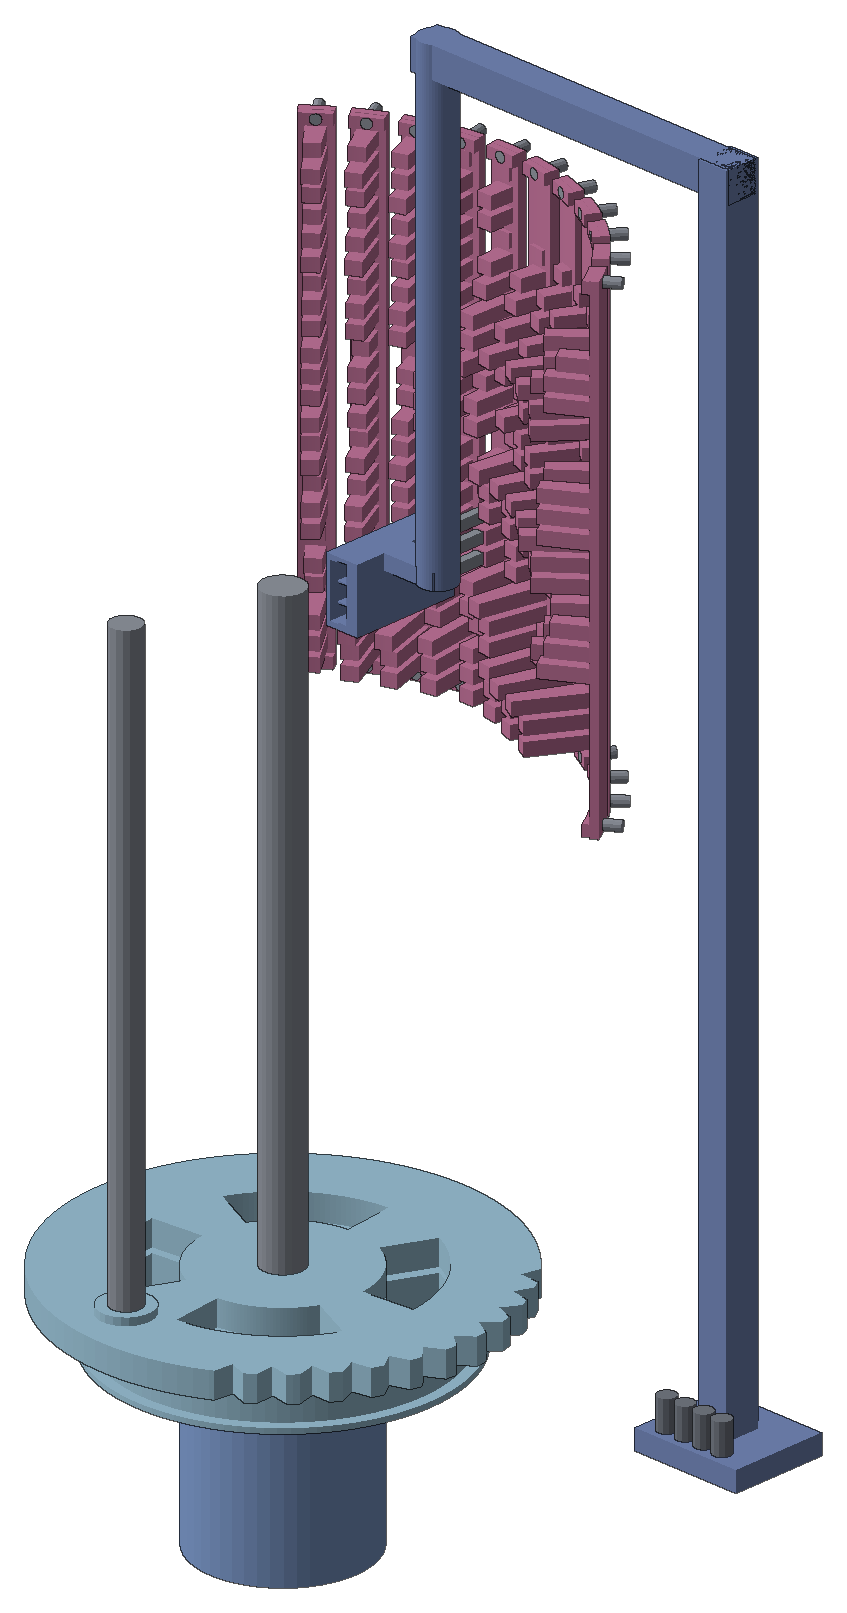
\includegraphics[width=0.49\linewidth]{gen/model/renders/read_head.png}\hfill
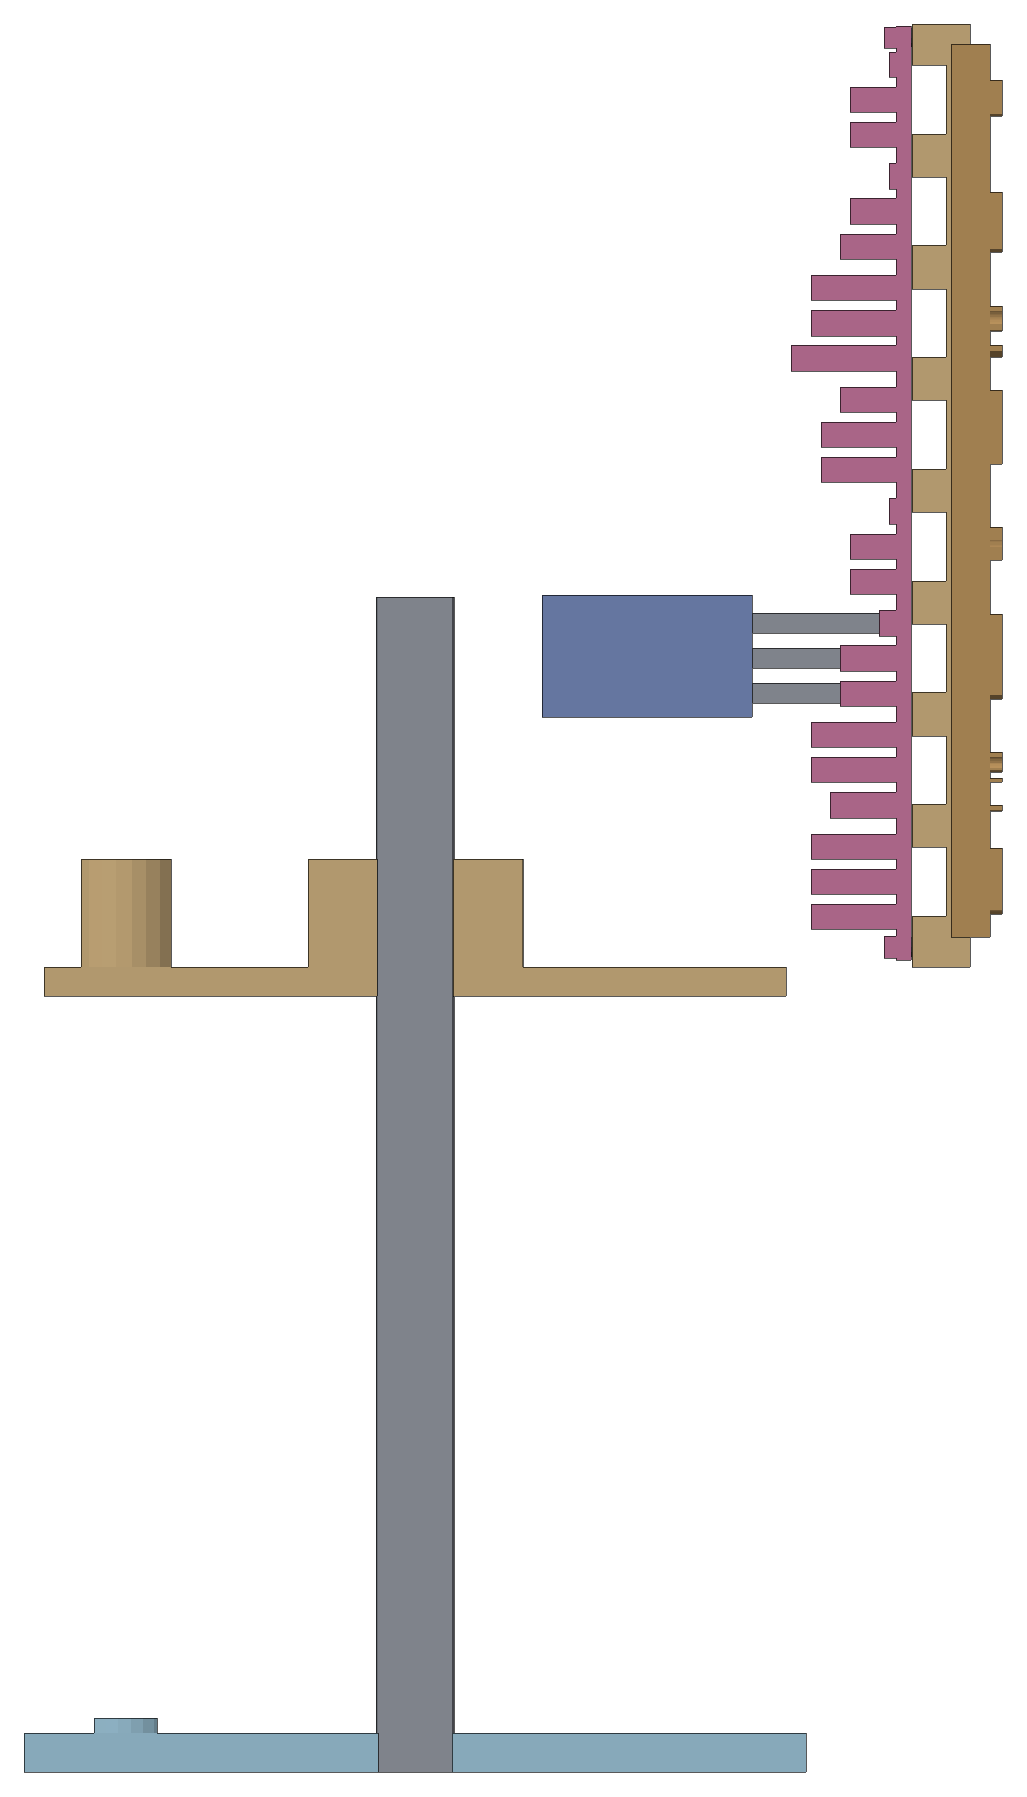
\includegraphics[width=0.49\linewidth]{gen/model/renders/read_cut.png}
\caption{Чтение кода в модели. Слева — челнок в момент чтения (позиция 4, ряд 6: ext. ando, $w = 15$, $b = c = 7$), кольцо и блоки сняты: гребёнки на кольце, головка с тремя щупами на своих зубцах, стойка головки и её кронштейн над челноком. Справа — разрез по оси удара: вал, поводок за валом, головка перед ним, щупы W, B, C до зубцов клетки.}
\label{fig:read}
\end{figure}

\begin{figure}[H]
\centering
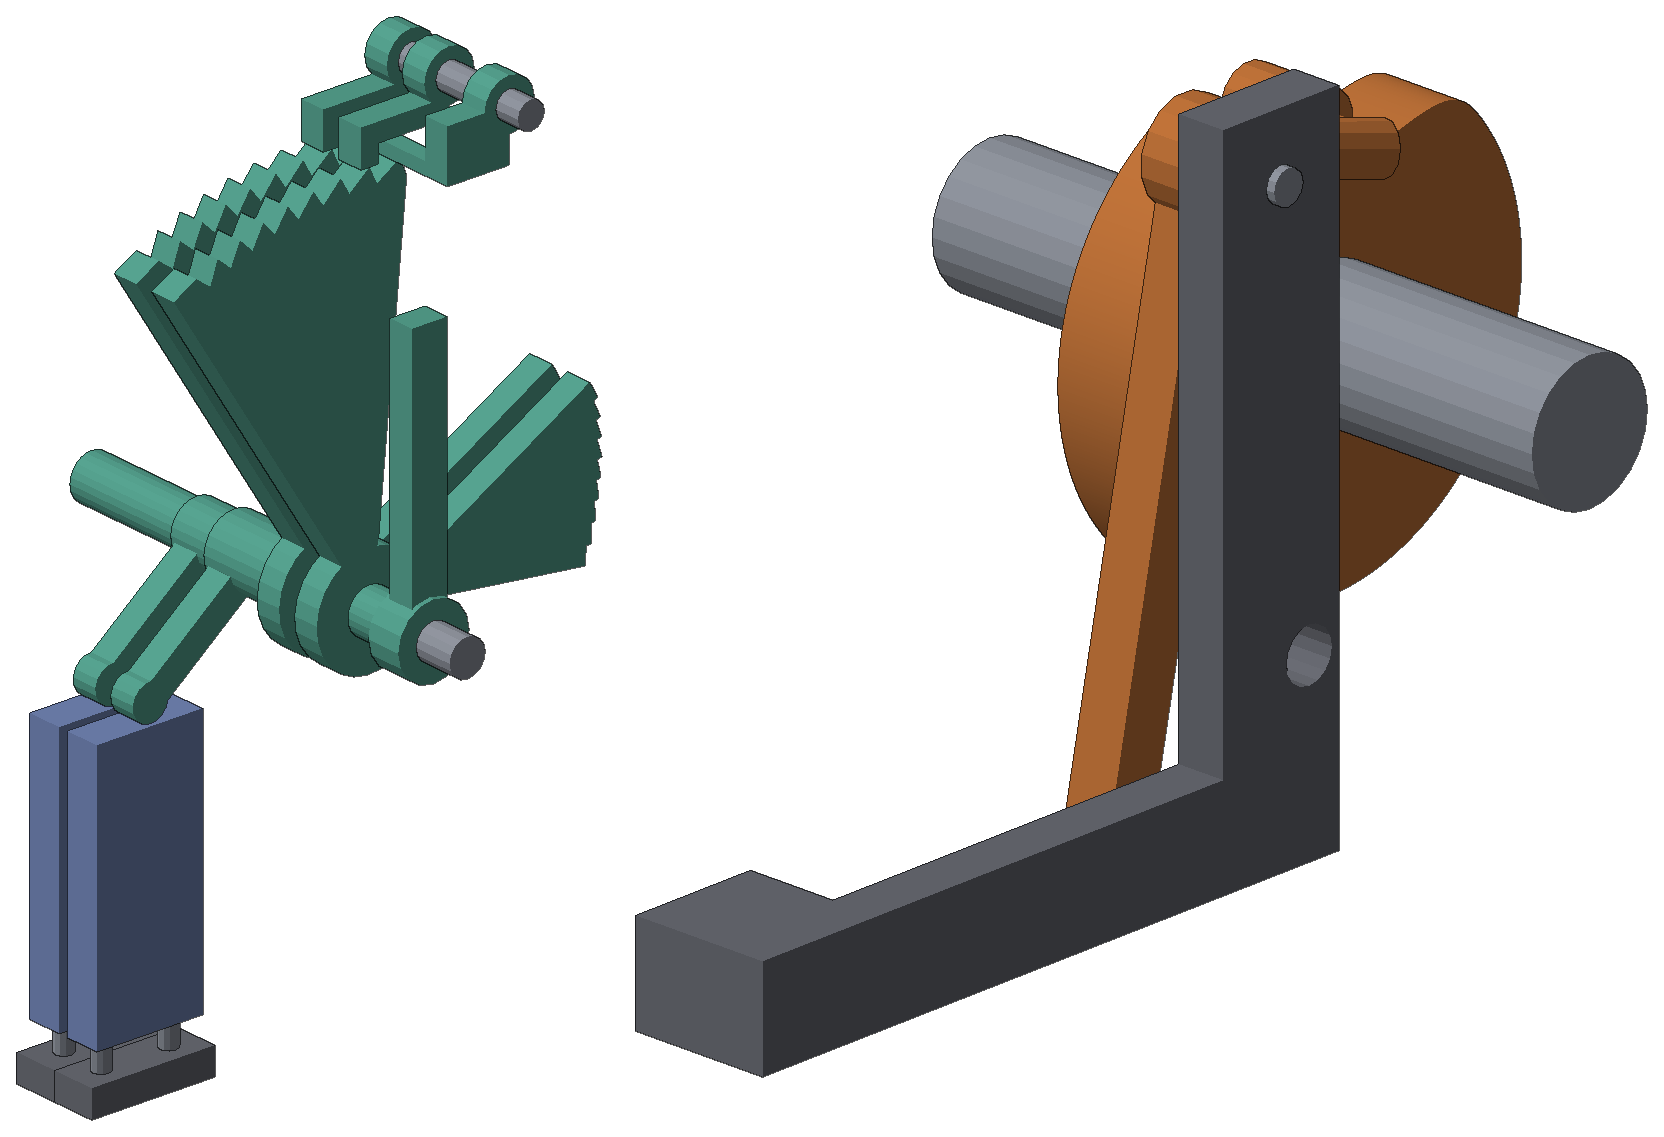
\includegraphics[width=0.49\linewidth]{gen/model/renders/read_slides.png}\hfill
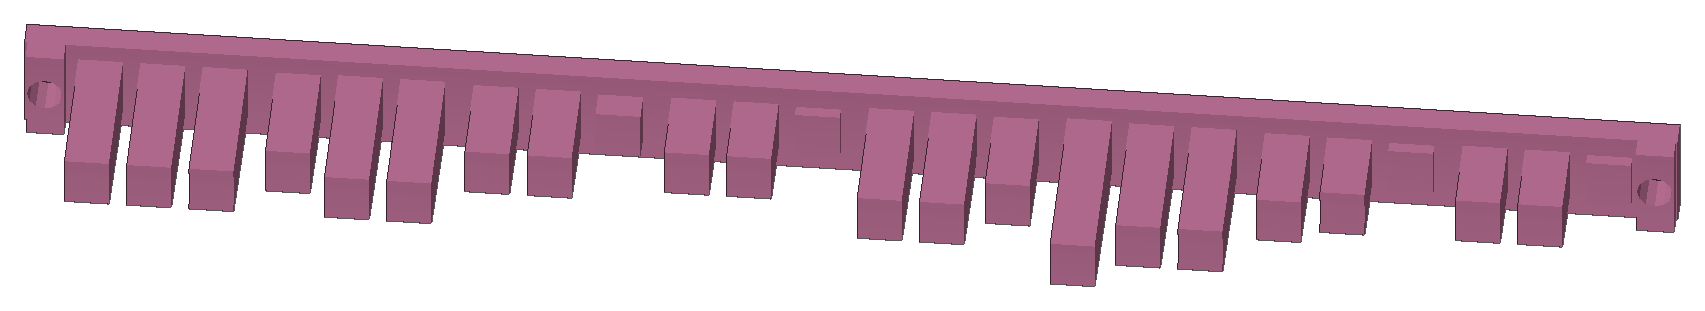
\includegraphics[width=0.49\linewidth]{gen/model/renders/read_comb.png}
\caption{Слева — ползунки B и C под роликами повторителей секторов (сектора держат считанные 7 и 7) и кулачок чтения с коромыслом. Справа — гребёнка позиции 4 так, как её печатают: на ребре.}
\label{fig:readparts}
\end{figure}

\paragraph{Проверка на модели.} Для каждой из \rdn\ продвигающих литер модель ставит её клетку на ось удара и пускает из конца каждого щупа девять лучей вдоль оси: все должны встретить один и тот же зубец, и ход должен быть ровно $c_0 + k\,v$ (сбоев: \rdbad). В сценариях на пересечения добавлены чтение каждой клетки (щупы на полпути и на зубцах, ползунки и тяга с ними) и чтение в цикле; в проверку касаний — ролик коромысла на кулачке, щупы на зубцах, ползунки под роликами, собачка задвижки (\S\ref{sec:contacts}). Интерактивная страница двигает щупы, ползунки, тягу W и коромысло по тем же законам; сверка страницы с моделью (\code{tools/web/compare\_model.py}, теперь и в состояниях чтения) расходится в них меньше чем на 0,1~мм. Больше расходятся только лента и палец упора U: страница рисует ленту неподвижной и считает палец введённым при любой ширине. Это упрощение было и в 0.9.3, но тогда сверка не ставила ширину и его не видела.

\paragraph{Цена.} Гребёнки весят \rdmass~г и добавляют \rdI~кг$\cdot$мм$^2$ к моменту инерции поворотной части (теперь \rdIrot~кг$\cdot$мм$^2$, подъёмная масса — \rdmlift~г). Щупы отдают валу на выходе то, что их пружины не тратят на нагрузку, и забирают полную работу пружин на возврате; за знак в среднем \rdEavg~мДж, до \rdEmax~мДж у самых широких литер. Вместе с инерцией гребёнок это подняло момент на цикловом валу до \mtauC~мН$\cdot$м и энергию на знак до \mEchar~мДж (было 101); знаков на завод — около \mcharswind. Палец, наоборот, разгружен: работа клавиши — 3,6~мДж вместо 12,3 (\S\ref{sec:forces}).

\paragraph{Что не построено.} Внутри головки, стойки и кронштейна тросы идут по роликам, которых в модели нет; оболочки тросов от стойки к приёмникам и к кулачку проложены по раме на бумаге, в модели стоят только их наконечники. Связь собачки задвижки с запорной гребёнкой дана положением. Пружины щупов и ползунков даны силами; жёсткость и трение тросов нужно замерить на стенде Э2.

\subsection{Спуск}

Колесо спуска связано через шестерню с рейкой каретки; пружинный двигатель каретки всё время стремится его повернуть. Зуб колеса соответствует одной единице хода каретки — 0,529~мм; передаточное число от колеса к рейке позволяет печатать и колесо, и рейку с крупным зубом.

\begin{figure}[h]
\centering
\begin{tikzpicture}[x=1mm,y=1mm]
\def\R{22}
\draw[mech,fill=gray!6] (0,0) circle (\R);
\foreach \i in {0,...,39} {\draw[ink!70] ({90+\i*9}:\R) -- ({90+\i*9+4.5}:{\R+2.2}) -- ({90+(\i+1)*9}:\R);}
\fill (0,0) circle (1.2);
\node[lbl] at (0,-5) {колесо спуска};
\draw[arr] (-8,10) arc (130:60:12) node[lbl,above right]{пружина каретки};
\draw[mech,fill=white] (-1.5,{\R+2.4}) -- (1.5,{\R+2.4}) -- (0,{\R-0.5}) -- cycle;
\draw[mech] (0,{\R+2.4}) -- (0,{\R+12}); \node[lbl,anchor=south] at (0,{\R+12}) {держащая собачка Д};
\def\ang{0}
\draw[thinmech,ink!40] (0,0) -- ({\ang}:{\R+8});
\draw[mech,fill=dead] ({\ang}:{\R-0.5}) -- ({\ang+3}:{\R+3}) -- ({\ang-3}:{\R+3}) -- cycle;
\node[lbl,anchor=west] at ({\ang}:{\R+5}) {переставной упор У};
\draw[{Latex[length=1.8mm]}-{Latex[length=1.8mm]},thick,draw=accent] (90:{\R+5}) arc (90:{\ang+4}:{\R+5});
\node[lbl,text=accent] at (45:{\R+10}) {$w$ зубьев};
\draw[mech,fill=gray!15] (-42,-14) circle (5); \node[lbl,anchor=north] at (-42,-20) {шестерня (на валу колеса)};
\draw[mech,dashed,ink!50] (0,0) -- (-42,-14);
\draw[mech] (-64,-8.6) -- (-22,-8.6);
\foreach \x in {-64,-62,...,-24} {\draw[ink!60] (\x,-8.6) -- (\x+1,-6.8);}
\node[lbl,anchor=south] at (-50,-6.5) {рейка каретки};
\node[lbl,anchor=north west,align=left,text width=56mm] at (30,-12) {
\textbf{При отпускании клавиши:}\\
1. Д выходит из зуба;\\
2. колесо идёт до упора У ($w$ зубьев);\\
3. Д падает в зуб;\\
4. палец У выходит из зубьев, У возвращается в ноль.};
\end{tikzpicture}
\caption{Спуск. Планка W отводит упор У на $w$ зубьев вперёд; при отпускании каретка проходит ровно $w$ единиц. Мёртвые знаки упор не трогают.}
\label{fig:esc}
\end{figure}

\subsection{Холостой цикл}
\label{sec:idle}

Каждое нажатие спускает цикловой вал. Для продвигающей литеры цикл читает код её клетки и бьёт; для мёртвого знака он должен бить, но не читать (кода у знака нет, а память нужна этому же циклу для отвода); для пробела — ни читать, ни бить. Пробел с 0.11 несёт разряды r1 и r4 (\S\ref{sec:spacepush}), поэтому челнок на его цикле не поворачивается, а только опускается к первому ряду средней позиции: без запора молоток ударил бы стоящую там техту, а щупы — после продвигающей литеры — прочли бы чужой код. В 0.10 у пробела разрядов не было вовсе, и челнок ходил к позиции 0. В 0.10 это было только описано; в 0.11 построены два запора (рис.~\ref{fig:idle}).

\begin{itemize}
  \item \textbf{Запор чтения} — стальной штырь Ø3 с головкой в направляющей на кронштейне коромысла чтения. Введённый, он стоит в 0,24~мм перед нижним плечом коромысла, пока кулачок держит коромысло поднятым (в покое). Когда в 118° кулачок опускается, коромысло остаётся на штыре, ролик отходит от кулачка, и щупы не выходят. Штырь вводит рычажок 9/9~мм на вертикальной оси; его второе плечо тянут два троса — от повторителя рамки О (мёртвые знаки) и от повторителя рамки W (пробелы); паз в плече принимает любой из них.
  \item \textbf{Запор удара} — такой же штырь в направляющей на стойке молотка, справа от молотка (слева проходит торцевая стенка каретки). Введённый, он стоит в 0,25~мм перед плечом молотка. В 160° взводной рычаг отпускается и бьёт губой по хвосту молотка; молоток уходить некуда, и работа пружины уходит в резиновую втулку штыря. Рычаг остаётся на хвосте молотка, как в покое, — запоздалого удара нет. Ленту на цикле пробела вибратор поднимает как обычно: без удара она не пачкает. Трос — от повторителя W.
\end{itemize}

Оба троса тянутся, пока клавиша нажата, то есть с начала хода пластины до её возврата, — дольше всего цикла. В модели штыри, рычажки, оси и направляющие — детали; проверено касание рычажков с головками (\S\ref{sec:contacts}) и оборот вала через 10° для знака над строкой, знака под строкой и пробела с введёнными запорами: пересечений нет (\S\ref{sec:checks}). На странице модели пробел теперь тоже идёт холостым циклом. Трассы тросов от повторителей О и W, как и у тросов чтения, — на бумаге.

\begin{figure}[H]
\centering
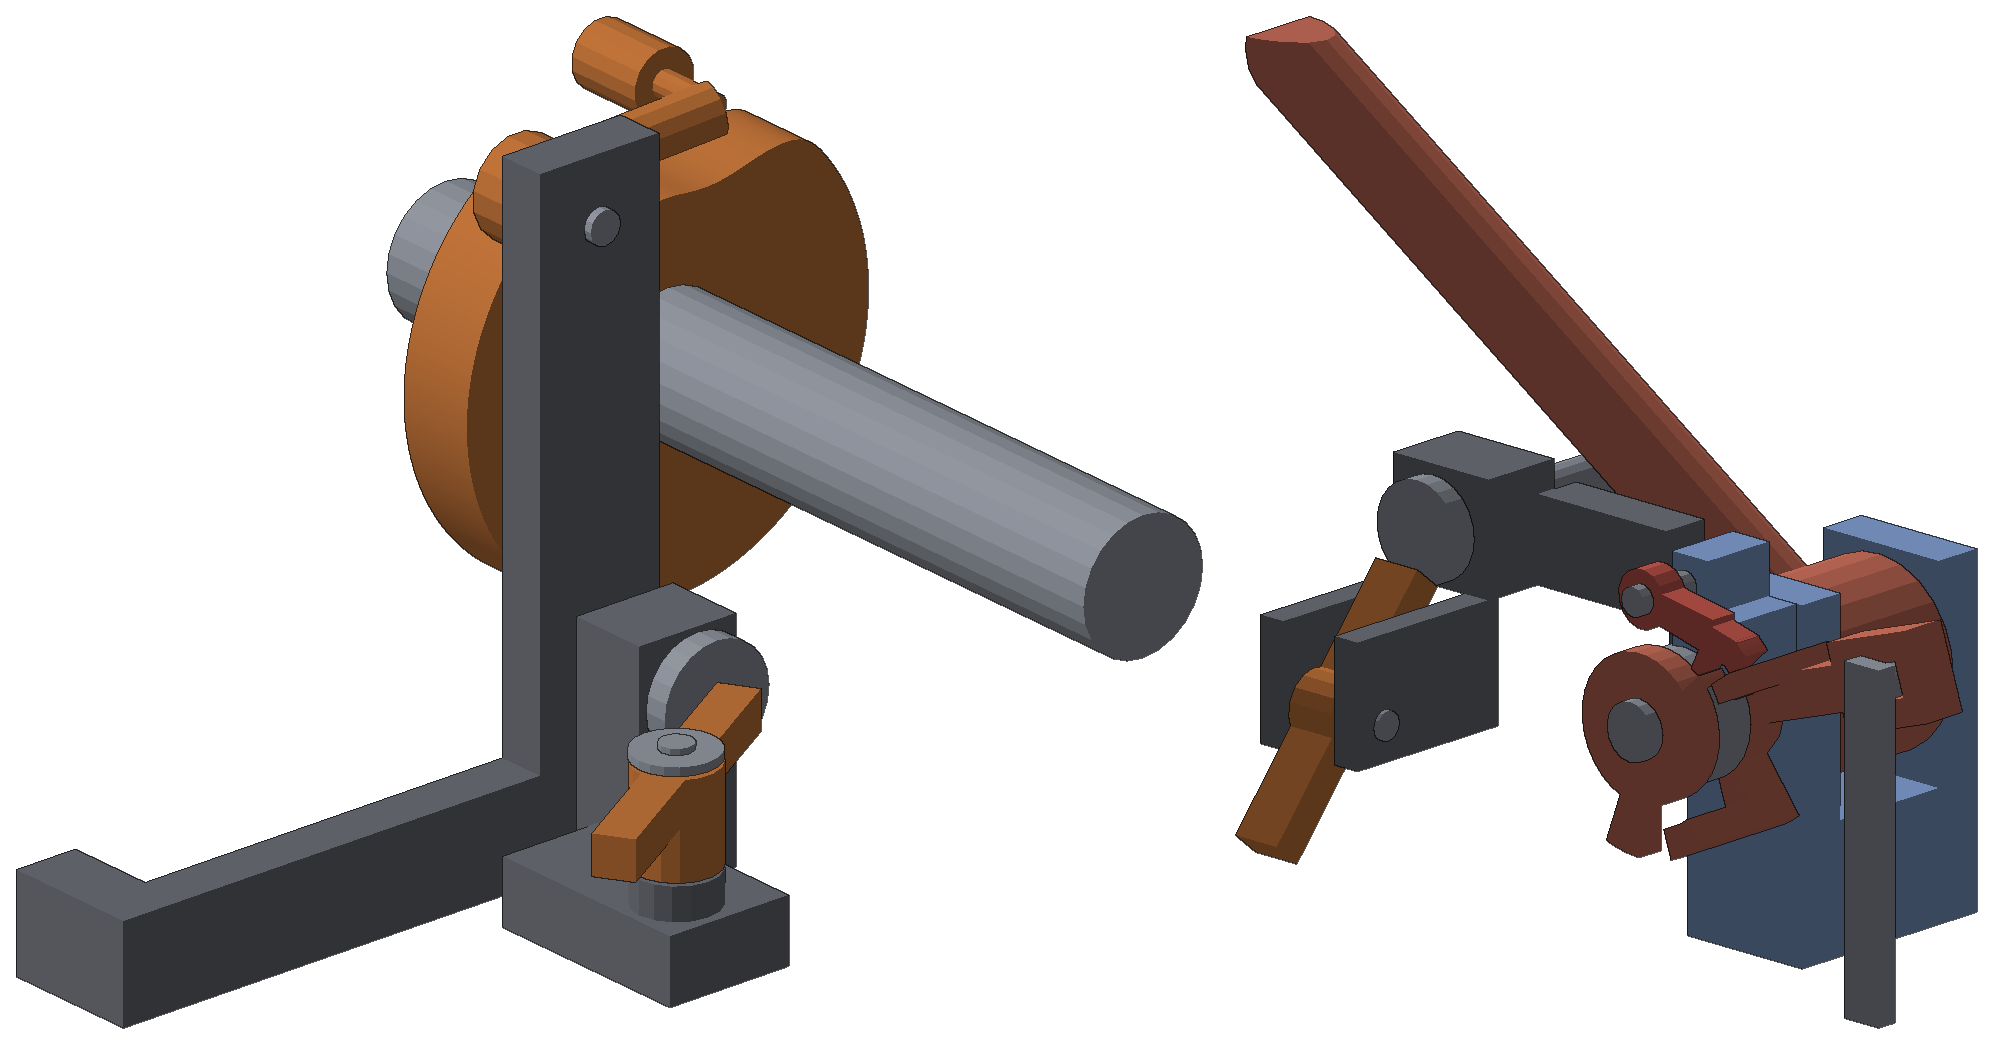
\includegraphics[width=0.92\linewidth]{gen/model/renders/idle_locks.png}
\caption{Холостой цикл в модели, пробел в 145°. Слева — запор чтения: кулачок опущен, коромысло стоит на штыре (под ним рычажок на вертикальной оси). Справа — запор удара: штырь в направляющей перед плечом молотка, рычажок на головке штыря, за ним взводной рычаг.}
\label{fig:idle}
\end{figure}

\paragraph{Цена.} Цикл пробела — полный оборот вала, и завода он тратит столько же, сколько литера. В текстах книг (\S\ref{sec:freq}) пробелы — \fqSP\,\% всех нажатий, поэтому знаков текста на завод на треть меньше, чем нажатий. Расчёт двигателя учитывает пробелы вместе с литерами (\S\ref{sec:motor}). Пробел, который отпускает спуск каретки сам, без цикла, как в обычной машинке, сберёг бы всю эту треть, но потребовал бы своего пути от клавиши к собачке спуска.

\paragraph{Толкатели пробелов.}\label{sec:spacepush} Пока у пробела не было разрядов, его холостой цикл гнал челнок к позиции 0 — на пять шагов поворота и обратно, а это самый тяжёлый поворот. Под хвостами рычагов пробелов поставлены два толкателя, такие же, как толкатели столбцов, но с выступами только под планками r1 и r4; планки разрядов позиции удлинены влево на 5~мм, до рычага пробела 4u, а направляющая толкателей — на оба рычага пробелов. Теперь пробел выбирает позицию 5, на которой челнок и так стоит в покое, и холостой цикл только опускает его к первому ряду. Момент на цикловом валу упал с 18,5 до \mtauC~мН$\cdot$м, энергия на нажатие — со 116 до \mEchar~мДж, нажатий на завод — около \mcharswind\ вместо 950. Касание рычагов пробелов с толкателями и толкателей с планками проверено так же, как у клавиш литер.

\subsection{Наборы шрифтов}
\label{sec:fontsets}

Шрифт задаёт только литерные блоки и кодовые гребёнки, поэтому для другого шрифта нужен другой набор из 22 деталей — больше ничего (с 0.11 и для шрифтов в раскладке Дэна Смита). Цепочка та же, что для Alcarin: \code{tools/fontprof.py} снимает шрифт, \code{tools/model/fontset.py} строит набор, проверяет его и выгружает STL и данные страницы (\code{make fonts}). Порядок такой.

\begin{enumerate}
  \item \textbf{Кегль.} Шрифт приводится к высоте тела Alcarin (верх коротких тенгв, 0,412~em). Если при этом какой-то код или рисунок выходит из пределов механизма, перебираются масштабы от 0,8 до 1,1 и берётся ближайший к 1, при котором всё ложится.
  \item \textbf{Оси.} Ось техт и нижняя ось каждой литеры берутся из якорей GPOS шрифта (связка «знак к основе» для гласных техт и для точек снизу); у шрифтов в раскладке Дэна Смита якорей нет, и оси определяются иначе (ниже). Коды — по тем же правилам, что у Alcarin: $a$ и $b$ — округлённые расстояния от левого края клетки до оси и от оси до правого края, $c = b - d$.
  \item \textbf{Подгонка.} Носители уже 4\,u дополняются до $w = 4$ (наименьший шаг спуска) с той же осью. Литера, рисунок которой заходит левее окна молотка, сдвигается в клетке вправо на целые единицы. Цифра, знак препинания или техта, которые выше окна по вертикали, рисуются меньше, а не весь шрифт.
  \item \textbf{Проверка.} Окно молотка — общее для всех наборов (молоток один); с 0.11 оно по высоте от $-4{,}2$ до $+6{,}6$~мм от линии шрифта (у Alcarin оттиск — от $-2{,}85$ до $+6{,}13$), чтобы вошли длинные стволы других шрифтов, а соседние ряды челнока остаются в 0,63~мм от лица. Рисунок после наращивания тонких мест должен лечь в окно. Гребёнки проверяются лучами для каждой продвигающей литеры, удар — для каждой клетки, ровно как у Alcarin (\S\ref{sec:read}, \S\ref{sec:strike}).
\end{enumerate}

\begin{center}\small
\setlength\tabcolsep{3pt}
\begin{tabularx}{\linewidth}{@{}Xrcccrrrrrcc@{}}
\toprule
Шрифт & кегль & $w$ & $b$ & $c$ & доп. & сдв. & умен. & г & кг$\cdot$мм$^2$ & чтение & удар \\
\midrule
\tabinput{gen/tab_fonts.tex}
\bottomrule
\end{tabularx}
\end{center}

\noindent{\small Кегль — к высоте тела Alcarin; доп. — носители, дополненные до 4\,u; сдв. — литеры, сдвинутые в клетке; умен. — знаки, нарисованные меньше; масса и момент инерции — 11 гребёнок. Hanno, Nenya, Miriel, Racina, Pixel, Comixanesse — Shankar Sivarajan (Miriel — по Tengwar Tellepsalinnacontar, Racina — по Tengwar Gothika, Hanno — по Baloo~2); Annatar — Johan Winge; Parmaitë, Eldamar и Tengwar Eldamar — Måns Björkman; Reformalized — Jakob Teuber; Formal CSUR — Michał Nowakowski; FreeMono Tengwar — GNU FreeFont.}

Все \fsOk\ наборов из \fsN\ прошли проверки чтения и удара. Гребёнки у других шрифтов тяжелее: у узких шрифтов (Miriel) коды меньше, зубцы длиннее; самая тяжёлая — на \fsIdelta~кг$\cdot$мм$^2$ больше, чем у Alcarin, это около 4\,\% момента поворотной части и меньше процента энергии на знак. Регулировка при смене набора — та же, что при сборке: нули трёх каналов чтения (\S\ref{sec:adjust}).

\paragraph{Шрифты в раскладке Дэна Смита.} Annatar, Parmaitë, Reformalized и другие шрифты этой раскладки сидят на клавишах ASCII и Latin-1 (одна карта для всех: tinco на «1», a на «\#», «E», «D», «C» и так далее) и якорей не имеют: пишущий сам выбирает одну из четырёх ширин каждой техты — широкую, обычную, узкую, самую узкую, — а техта, знак нулевой ширины, нарисована левее своего начала и ложится на предыдущую букву. Значит, каждая ширина даёт для буквы готовую ось: ширина буквы плюс смещение техты. Ось буквы — та из четырёх, что ближе всего к середине её рисунка в верхней половине тела (\code{fontprof.raw\_ds}); так же нижняя ось — по четырём ширинам точки снизу и рисунку нижней половины. Одна геометрия ошибается: на шрифтах с якорями она промахивается мимо настоящей оси на 0,6--1,3\,u в среднем и до 2,5\,u у отдельных букв; привязка к ширинам, заданным автором шрифта (они стоят через 2--3\,u), снимает почти всё. Мёртвые знаки на челноке — обычной ширины, долгие гласные «ára + гласная» — той ширины, что подходит ára. Листы \code{tools/fontaxes.py} рисуют каждую букву шрифта с её осями — по ним видно, что техты встают над луком, а у двухлуковых букв — между луками. Так легли Annatar, Annatar Bold, Parmaitë и Reformalized (рис.~\ref{fig:dsaxes}); в Dan Smith-шрифтах нет sa-rincë и метки младшего разряда — эти клетки пустые.

\begin{figure}[H]
\centering
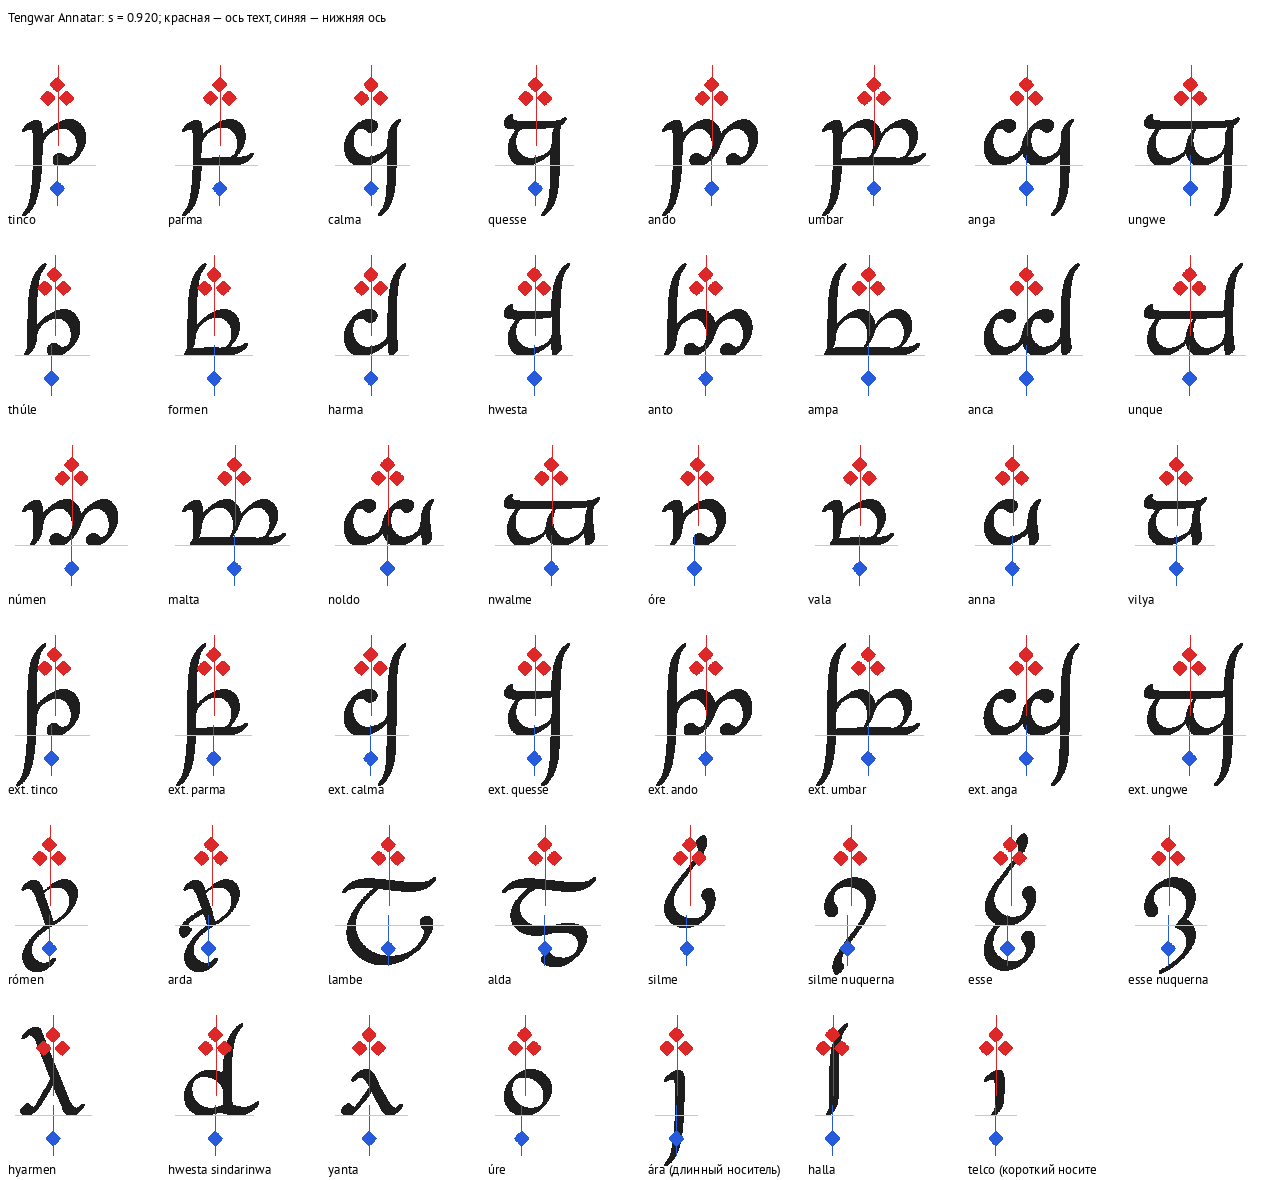
\includegraphics[width=0.9\linewidth]{gen/fonts/annatar/axes.png}
\caption{Оси литер Tengwar Annatar, найденные по ширинам её техт: красным — техта a над осью техт, синим — точка снизу под нижней осью, как их поставит челнок.}
\label{fig:dsaxes}
\end{figure}

\paragraph{Шрифты CSUR без якорей.} У Eldamar, Tengwar Eldamar, Tengwar Formal CSUR, FreeMono Tengwar и miue кодировка правильная, но якорей техт нет. Это не значит, что шрифт не знает, куда ставить техту: Eldamar выбирает сдвинутый вариант точки по предыдущей букве подстановкой GSUB (свой для двухлуковых, для lambe, для носителей), Tengwar Formal CSUR делает то же таблицей AAT \code{morx}, а FreeMono и miue ставят техту на одно и то же место после любой буквы (FreeMono моноширинный, так и задумано). Поэтому оси берутся у самого шрифта: HarfBuzz набирает букву с точкой (и букву с точкой снизу), и середина точки — ось, которую шрифт даёт (\code{fontprof.raw\_shaped}). Если она не над рисунком буквы или отходит от середины верхней половины тела на 3\,u и больше, ось оценивается по рисунку (как для шрифтов Дэна Смита, только без ширин). Так вышло у Tengwar Eldamar — шрифт старый, его техта стоит у правого края любой буквы, и все его оси оценены по рисунку (рис.~\ref{fig:shapedaxes}); у miue — четыре носителя. В Eldamar нижняя ось lambe лежит левее, чем достаёт сектор C (отвод 11\,u), — для неё знаки под строкой сдвинуты на 2\,u вправо. При замере нашлась и ошибка цепочки: составные глифы (у Formal CSUR так сделаны техты, у Nenya — знаки под строкой) масштабировались дважды; исправлено, все наборы перестроены.

\begin{figure}[H]
\centering
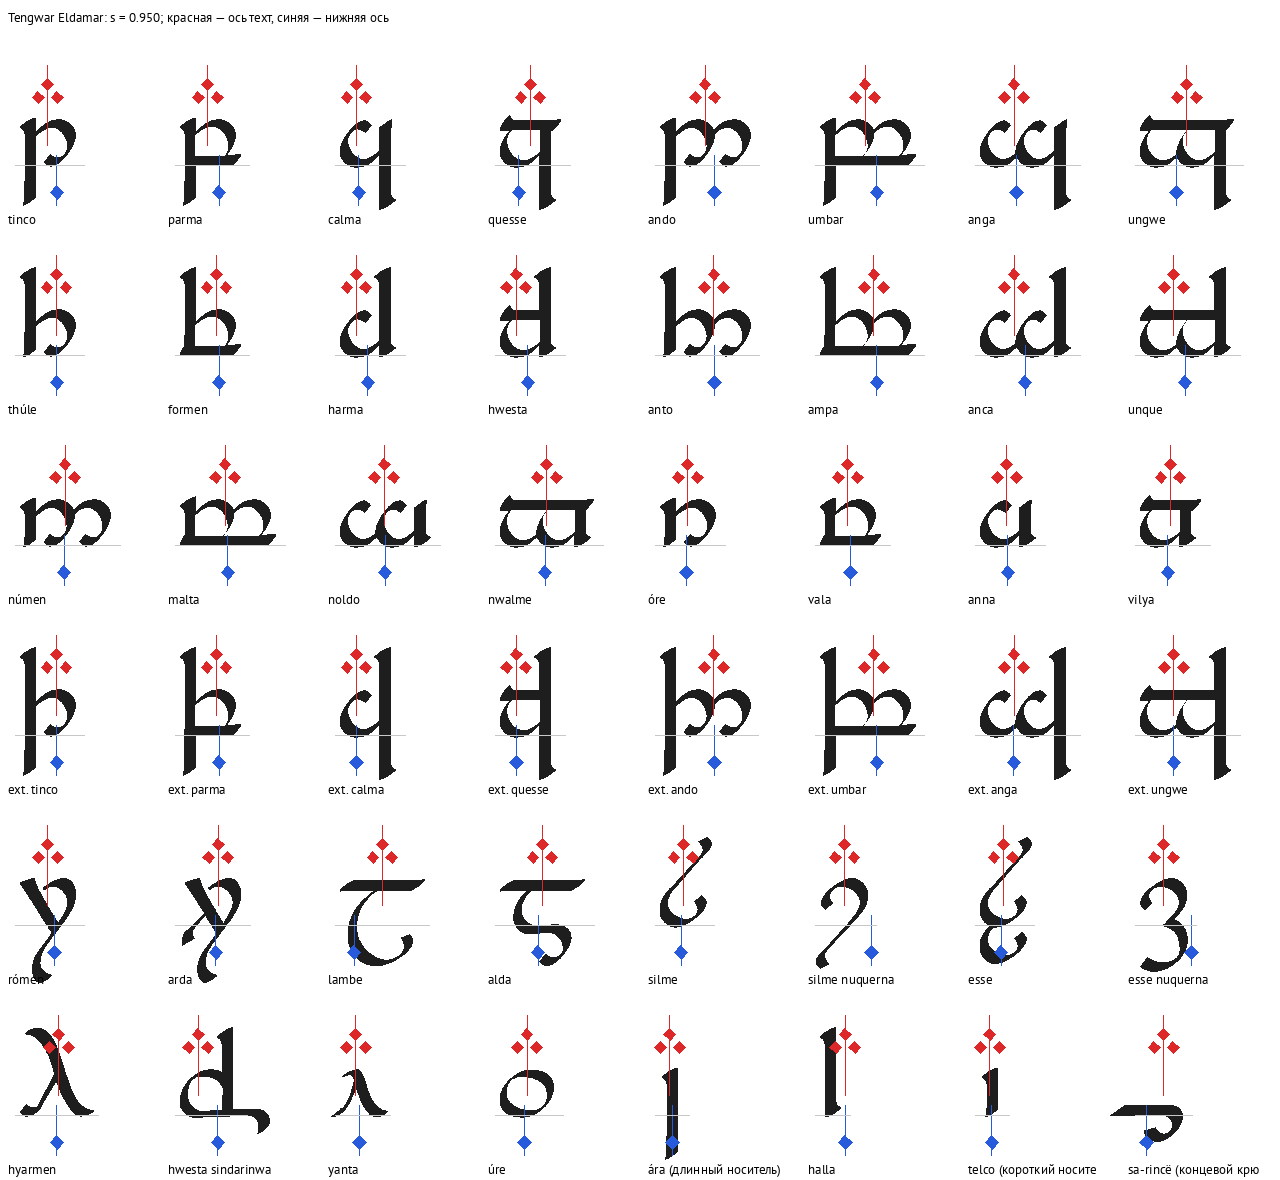
\includegraphics[width=0.9\linewidth]{gen/fonts/eldamar-old/axes.png}
\caption{Оси литер Tengwar Eldamar: шрифт сам техту не ставит, все оси оценены по рисунку буквы. Это наименее надёжный набор; лист нужно проверить глазом до печати блоков.}
\label{fig:shapedaxes}
\end{figure}

\paragraph{Какие шрифты не легли.} Курсивы Annatar слишком велики (литеры до 22\,u, стволы на 8~мм под строку). Balgruf размечен не по общей карте: оси выходят левее букв. Teleri ложится, но его права закрыты («all rights reserved»), и в репозиторий он не положен. Tengwar Artano слишком велик. В Oz's Wizard нет 14 знаков машинки, среди них носовых черт, точки снизу и кавычек.

\paragraph{Если знака в шрифте нет.} Механически это не беда: клетка остаётся пустой, а гребёнка всё равно несёт у неё зубцы — код узкого пробела ($w = 4$, $b = c = 0$). Пустая клетка без зубцов была бы опасна: щупы ушли бы до упора и поставили бы наибольшую ширину и отвод. Клавиша такого знака печатает пустое место в 4\,u, страница модели знак не печатает. Беда другая — текстовая: знак нельзя набрать; например, без носовых черт и точки снизу синдарин в общем режиме не пишется. Поэтому шрифт без части знаков допустим, но набор для него — неполный.

\paragraph{На странице модели} шрифт челнока выбирается в списке. Сцена не пересобирается: заменяются геометрии 22 деталей (блоки и гребёнки) и таблицы кодов и рисунков; данные каждого набора лежат в своём файле рядом со страницей и загружаются, когда набор выбран. Клавиши остаются с литерами Alcarin — они от шрифта не зависят. Набор меняется, когда машинка стоит.

\subsection{Память: два сектора}

Сектора B и C поворачивают ползунки B и C, которые тянут тросы щупов B и C (\S\ref{sec:read}); на дуге каждого сектора — зубчатый фиксатор и защёлка. Сектор B держит упор отвода для надстрочных знаков, C — для подстрочных. Сектор W с редакции 0.9.1 никем не читался (ширину последней литеры для «назад на литеру» держит рычаг памяти M спуска, \S\ref{sec:back}) и в 0.11 снят.

\begin{figure}[h]
\centering
\begin{tikzpicture}[x=1mm,y=1mm]
\fill (0,0) circle (1.2);
\draw[mech,fill=sledA!10] (0,0) -- (60:30) arc (60:120:30) -- cycle;
\foreach \i in {0,...,9} {\pgfmathsetmacro\a{114-\i*6}
  \draw[ink!70] (\a:30) -- (\a:32);
  \node[lbl,font=\sffamily\tiny] at (\a:35) {\i};}
\draw[mech,fill=white] (0,40) -- (2,32.5) -- (-2,32.5) -- cycle;
\draw[mech] (0,40) -- (0,46); \node[lbl,anchor=south] at (0,46) {защёлка};
\draw[mech] (0,0) -- (-30,-8);
\node[lbl,anchor=east] at (-30,-8) {от планки B};
\draw[mech,sledA,thick] (0,0) -- (40,-6) -- (70,-6);
\draw[mech,fill=sledA!60] (70,-9) rectangle (73,-3);
\node[lbl,anchor=west,text=sledA] at (74,-6) {упор $b$ ползуна};
\draw[arr] (-20,14) arc (150:125:22); \node[lbl,anchor=east] at (-20,14) {пружина к нулю};
\node[lbl,anchor=north west,align=left,text width=72mm] at (-35,-14) {
\textbf{На каждой продвигающей литере:} (1 — на ходу клавиши, 2 и 3 — в цикле, при чтении)\\
1. планка R клавиши поднимает защёлку, пружина возвращает сектор в ноль;\\
2. ползунок B (трос щупа) ведёт сектор на $b$ делений;\\
3. защёлка падает в ближайшую впадину и держит сектор.\\
\textbf{На мёртвом знаке} сектор не трогают: он служит упором.};
\end{tikzpicture}
\caption{Сектор памяти B. Сектора C и W устроены так же.}
\label{fig:mem}
\end{figure}

\subsection{Отвод печатающего узла}

При мёртвом знаке рамка О через тягу с пружиной отводит узел назад, пока щуп на узле не упрётся в ступень сектора B, а если ярус знака несёт выступ N, — сектора C. Тяга пружинная, поэтому положение задаёт ступень, а не глубина нажатия. После удара пружина возвращает узел на нулевой упор. Устройство — в \S\ref{sec:stops}.

\subsection{Служебные клавиши}

\begin{itemize}
  \item \textbf{Пробелы 4u и 6u} — постоянные пластины: $w = 4$ или $6$, память в ноль.
  \item \textbf{Забой} — колесо спуска назад на один зуб (1\,u). Память не трогает.
  \item \textbf{Назад на литеру} — храповой толкатель поворачивает колесо спуска назад до упора сектора W и сбрасывает память. Если затем ударить ту же литеру через корректирующую ленту, она ляжет на прежнее место, а память восстановится.
  \item \textbf{$\pm u$} — качающийся рычажок: пока он отклонён, нулевой упор ползуна смещён на единицу. Ручная поправка для редких случаев.
\end{itemize}

\subsection{Блокировки}

\begin{itemize}
  \item \textbf{Одна клавиша за раз.} Плавники рычагов проходят через шариковую дорожку: шарики оставляют место ровно одному плавнику.
  \item \textbf{Контроль полного хода.} Начатая клавиша должна дойти до конца: храповые собачки на рамках R и О не дают им вернуться, пока они не прошли 16~мм.
  \item \textbf{Очерёдность.} На время оборота цикла запорная гребёнка сдвигается на полшага и держит все рычаги; подробнее — в \S\ref{sec:links}.
\end{itemize}

%=====================================================================
\section{Проработка звеньев}
\label{sec:links}

В редакции 0.7 часть звеньев была дана в модели схематично — габаритами, без механизма. В редакции 0.8 они построены деталями, проверены на пересечения во всех состояниях движения и, где это возможно, рассчитаны (\code{tools/model/links.py}).

\subsection{Коромысла выбора}

\paragraph{Кулисы вместо шарниров.} Плавающий рычаг на двух шарнирах складывает ходы точно только при малых углах: концы описывают дуги, и точка выхода уходит вбок. Поэтому каждое звено дерева — ползун (стальная полоса 4$\times$3~мм) в прорези направляющей плиты, а рычаг соединён с ползунами пальцами в продольных пазах. Ползун разряда, ползуны узлов и выходной ползун ходят строго по прямой, и узел делит ход точно в отношении весов при любом угле рычага: $n_k = n_{k-1} + (b_k - n_{k-1})\,2^k/(2^{k+1}-1)$. Модель повторяет это до ошибки $10^{-14}$~мм. Положения ползунов вдоль плиты подобраны перебором так, чтобы соседние стержни выбора стояли не ближе 15~мм (у стержня палец шириной 13~мм).

\begin{center}\small
\begin{tabularx}{\linewidth}{@{}lXXccc@{}}
\toprule
& ползуны разрядов (1, 2, 4, 8), мм & узлы, мм & усиление & плечи, мм & сдвиг опоры, мм \\
\midrule
\tabinput{gen/tab_links_sel.tex}
\bottomrule
\end{tabularx}
\end{center}
\label{tab:ladder}

\noindent{\small Координаты — вдоль плиты от оси удара. Выходной рычаг второго рода: вход на коротком плече, опора — на ползуне, который двигает та же приводная планка; так из суммы вычитается постоянное смещение (для поворота — 5 позиций, для подъёма — от ряда покоя). Выход поворота — каретка ленты на MGN7, выход подъёма — ползун, угловой рычаг под плитой, толкатель и вилка подъёма (плечи 30 и 150~мм).}

\paragraph{Защёлки.} Над каждым ползуном разряда — палец 3~мм с пружиной вниз. Стержень выбора, поднятый планкой разряда, поднимает палец на 3,5~мм, и тот входит в вырез приводной планки; планка уводит ползун на 12~мм. Площадка пальца длиной 18~мм вдоль хода, поэтому палец не соскакивает со стержня, пока ползун идёт. Стержни выбора изогнуты: от планок разрядов у края клавиатуры они идут вверх, вдоль плиты и снова вверх к своему ползуну, обходя поле рычагов. Привод — 2,7~Н для поворота и 2,2~Н для подъёма на кулачке.

\begin{figure}[H]
\centering
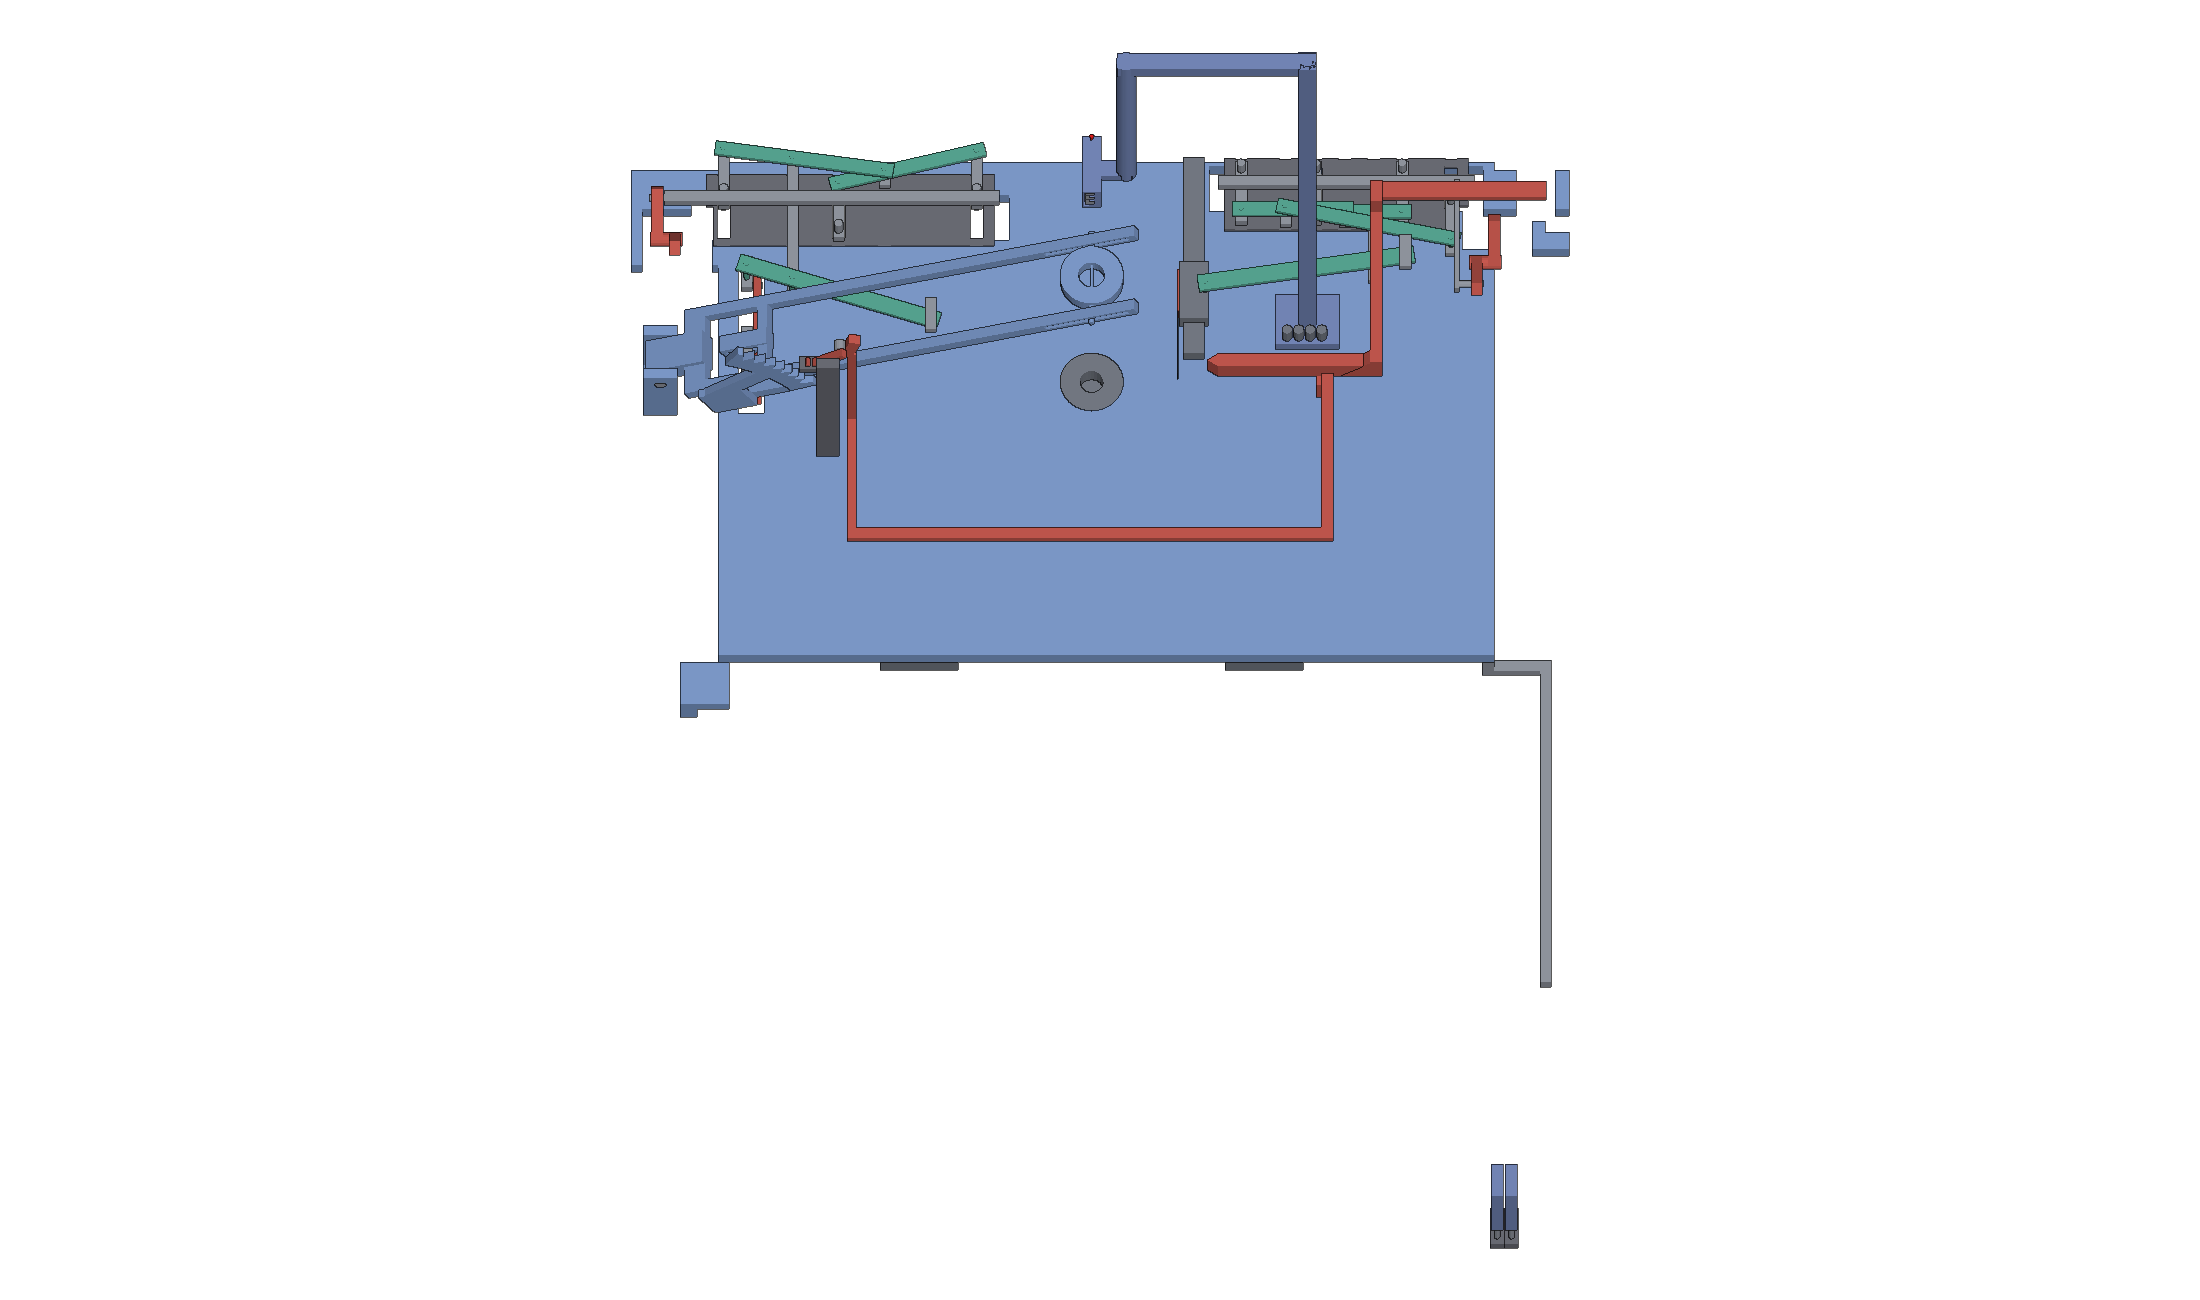
\includegraphics[width=0.9\linewidth]{gen/model/renders/select_unit.png}
\caption{Узел выбора на плите, вид сверху (код r8, l1, l4). Справа — дерево поворота: направляющая плита с ползунами разрядов и пальцами защёлок, коромысла (зелёные), выходной рычаг с опорой на подвижном ползуне, тяга к каретке ленты; слева — дерево подъёма и угловой рычаг к вилке. Красные — приводные планки и тяги от кулачков.}
\label{fig:selunit}
\end{figure}

\subsection{Мерные рамки}

Параллелограммы вложенных рамок не раскладываются: шарниры шести (с ред. 0.10 — четырёх: R, W, О, N) рамок пришлось бы ставить друг в друга. Поэтому рамка ходит поступательно по четырём вертикальным стальным пруткам 3~мм во втулках длиной 10~мм; при зазоре 0,05~мм перекос — 0,8~мрад. Передние прутки висят на кронштейне яруса, задние стоят на полосе основания; ярусные каретки сдвигаются вместе с рамками клавишей регистра. Каждую рамку несут две пружины, так что пластина толкает её с почти постоянной силой.

\begin{center}\small
\begin{tabular}{@{}lrrrrr@{}}
\toprule
рамка & дорожка $x$, мм & пруток, мм & масса, г & ход, мм & сила, Н \\
\midrule
\tabinput{gen/tab_links_frames.tex}
\bottomrule
\end{tabular}
\end{center}

\noindent{\small Дорожка — расстояние от оси машинки до места, где ролик повторителя лежит на балке рамки. Сила — от начала до конца хода (пружины рамки и повторителя).}

\subsection{Сектора памяти}

Сектора сидят на соосных латунных трубках 5, 6 и 7~мм (телескопический набор; с 0.11, когда снят сектор W, — три трубки вместо четырёх) на общей оси 4~мм, запрессованной в правую щёку двигателя. На каждой трубке — повторитель: рычаг 16~мм с роликом, лежащим на плоском верху балки своей рамки (у B и C с ред. 0.10 — на верху ползунка, который ходит на месте прежней балки). Так рамке безразличен сдвиг регистра вдоль машинки, а трубка поворачивается на угол, однозначно связанный с ходом рамки. Ход не пропорционален углу, поэтому зубья храповика нарезаны не равномерно, а там, куда приходит повторитель при ходе в $k$ единиц: $\theta_k = \arcsin\frac{h_0 + k}{r} - \theta_0$, $h_0 = 3$~мм. Шаг зуба на радиусе 42~мм — от 2,7 до 3,8~мм у B и C и до 6,3~мм у W. Три собачки на общей оси над секторами держат сектора; палец на трубке R поднимает их в первые 2~мм хода R (сброс на каждой продвигающей литере) и проходит мимо.

\begin{figure}[H]
\centering
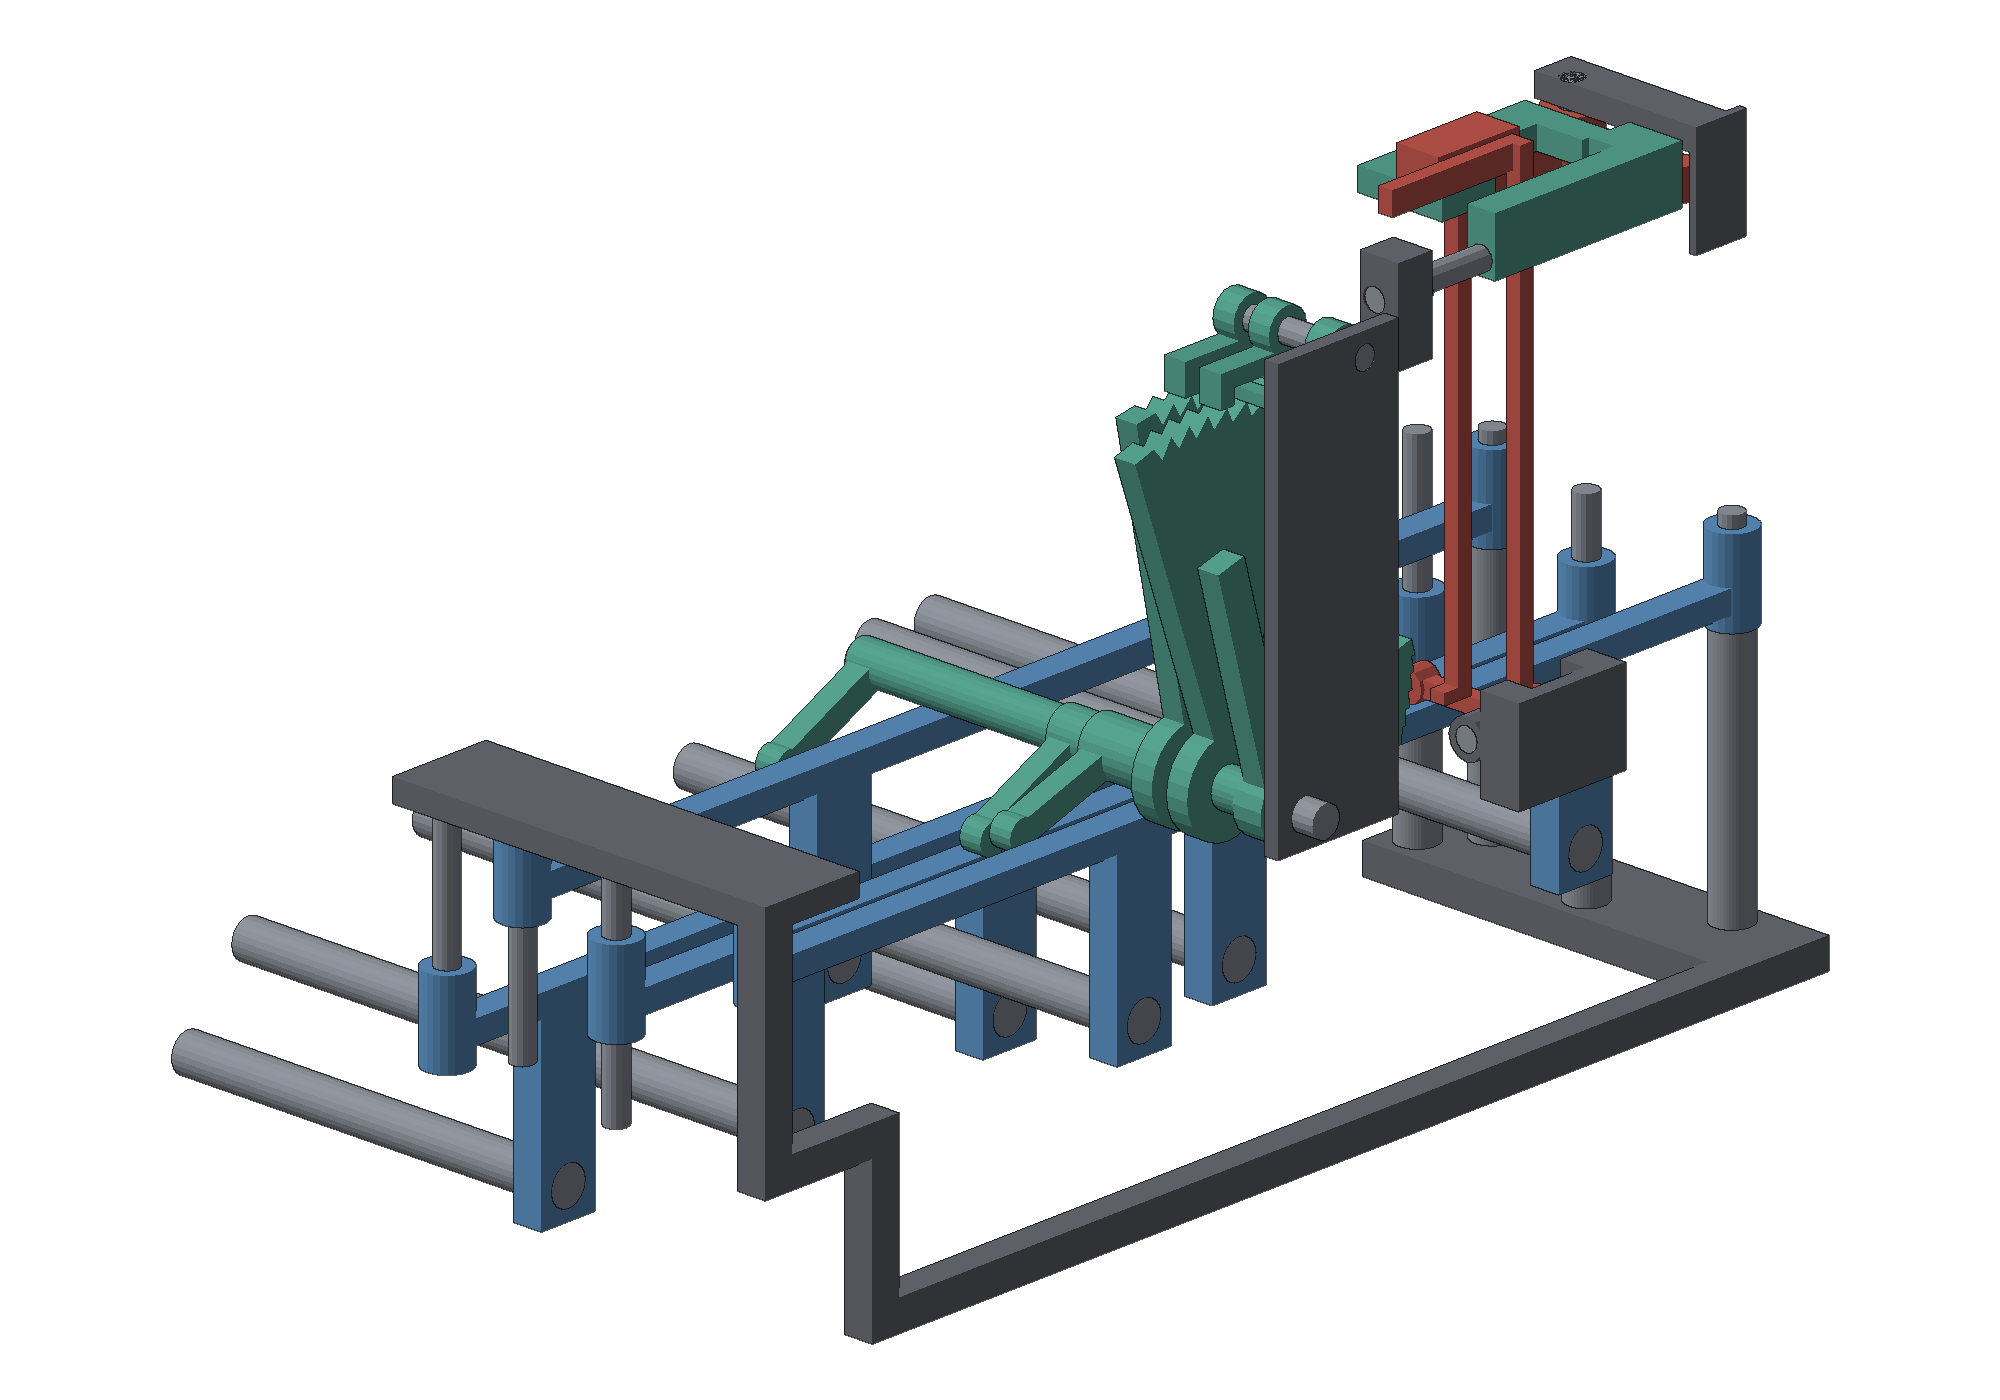
\includegraphics[width=0.8\linewidth]{gen/model/renders/frames.png}
\caption{Рамки на вертикальных направляющих и сектора памяти на соосных трубках у правой щеки двигателя (рамка R опущена на 16~мм, W — на 6; ползунки B и C — на 4 и 2~мм); повторители лежат роликами на балках рамок и на ползунках.}
\label{fig:frames}
\end{figure}

\subsection{Связь с упором спуска}

Упор спуска ставится тягой Y, которую ведут два источника: повторитель живой рамки W (пробелы, пока клавиша нажата) и трос щупа W (литеры, \S\ref{sec:read}); тяга идёт за тем, кто потянул дальше, а задвижка держит её до подачи. Слева от рамок стоит второй повторитель W — синусный рычаг: ролик на балке и ролик на площадке тяги под прямым углом, поэтому тяга проходит ровно столько, сколько рамка, без поправки на угол. Тяга 2~мм идёт вдоль левого края (\mescL~мм), угловой рычаг 1:1 с кулисами поворачивает её поперёк (\mescLL~мм) к рычагу упора на оси колеса спуска. Плечо рычага \mescra~мм даёт 6° на единицу — один зуб колеса из 60. Тяги работают только на растяжение, назад упор возвращает пружина у спуска — с ред. 0.10 0,2~Н вместо 0,5, чтобы щуп W тянул поменьше; удлинение тяги под ней — меньше микрона.

\subsection{Молоток и взвод}

Молоток (\mhmass~г, головка на радиусе 78~мм) отходит на 18° и бьёт со скоростью около \mhv~м/с; энергия удара — 20~мДж. Пружина кручения взводится рычагом на оси молотка с плечом \mhrcock~мм: кулачок поднимает толкатель на 6~мм с 10° по 150° (усилие \mhFcam~Н), на 160° его профиль обрывается, и молоток свободен. Тяга от толкателя к рычагу проходит под плитой узла и вдоль рычага рамы, поэтому отвод узла её не сбивает.

\begin{figure}[H]
\centering
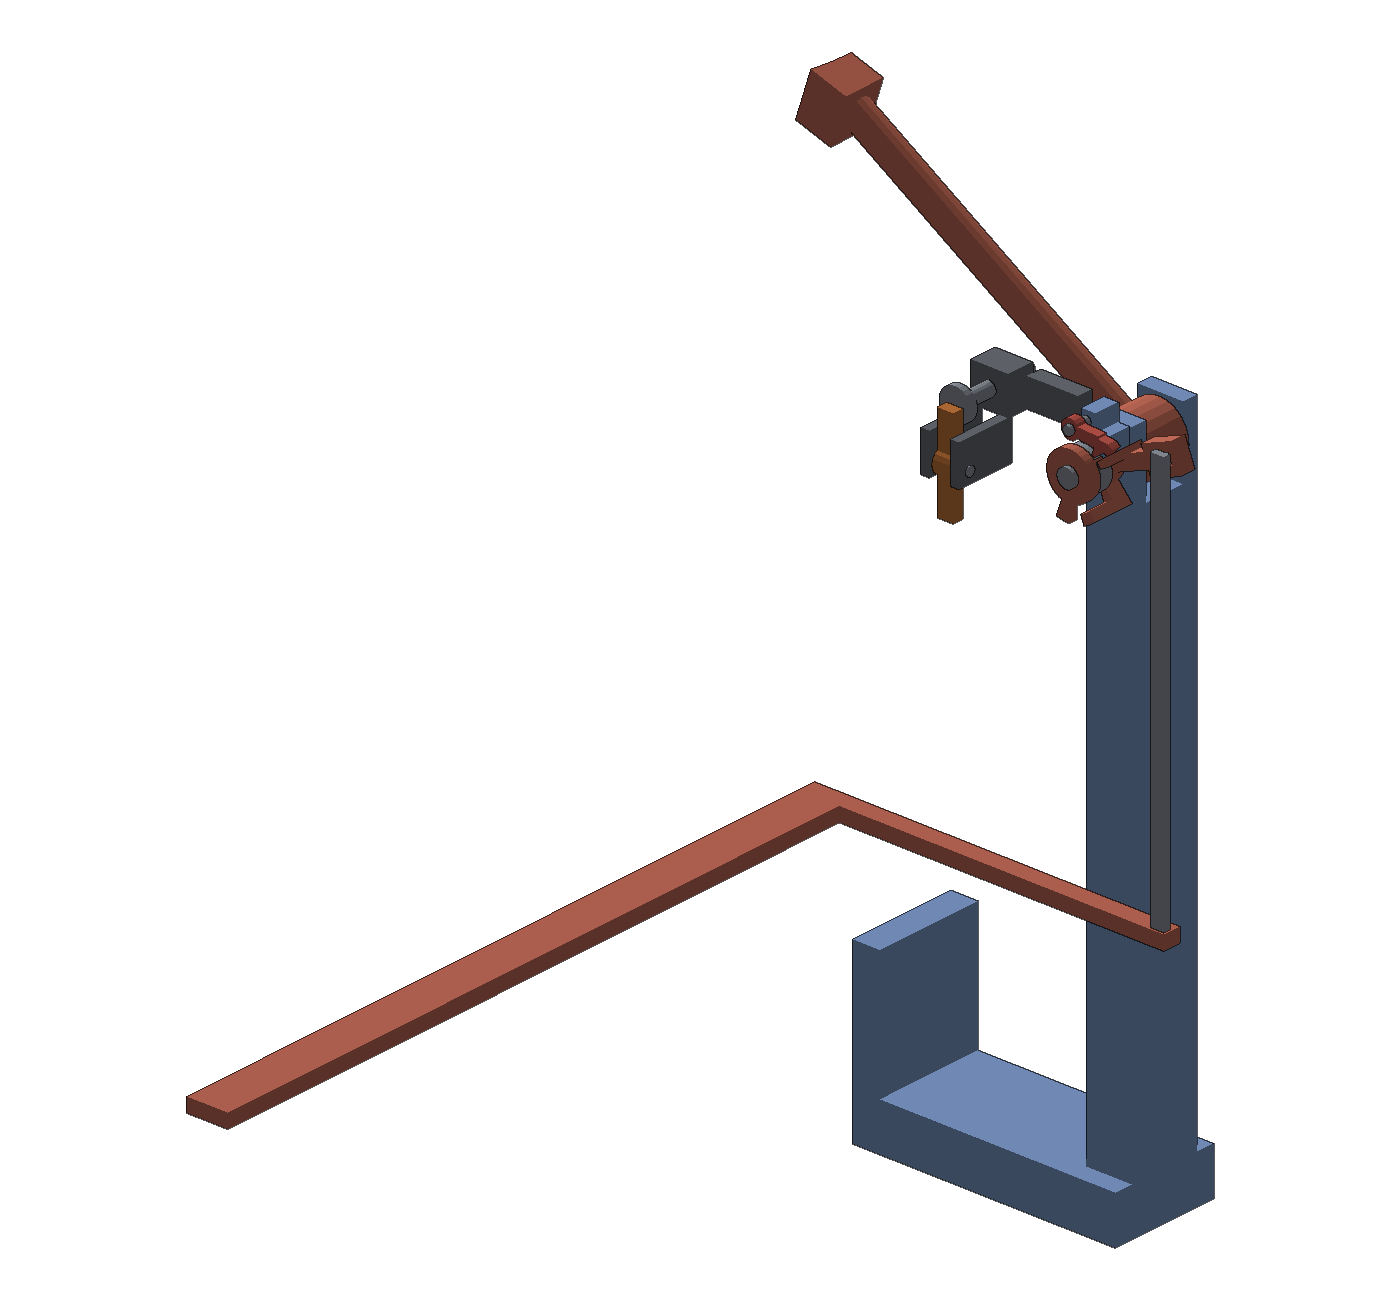
\includegraphics[width=0.48\linewidth]{gen/model/renders/hammer_cock.png}\hfill
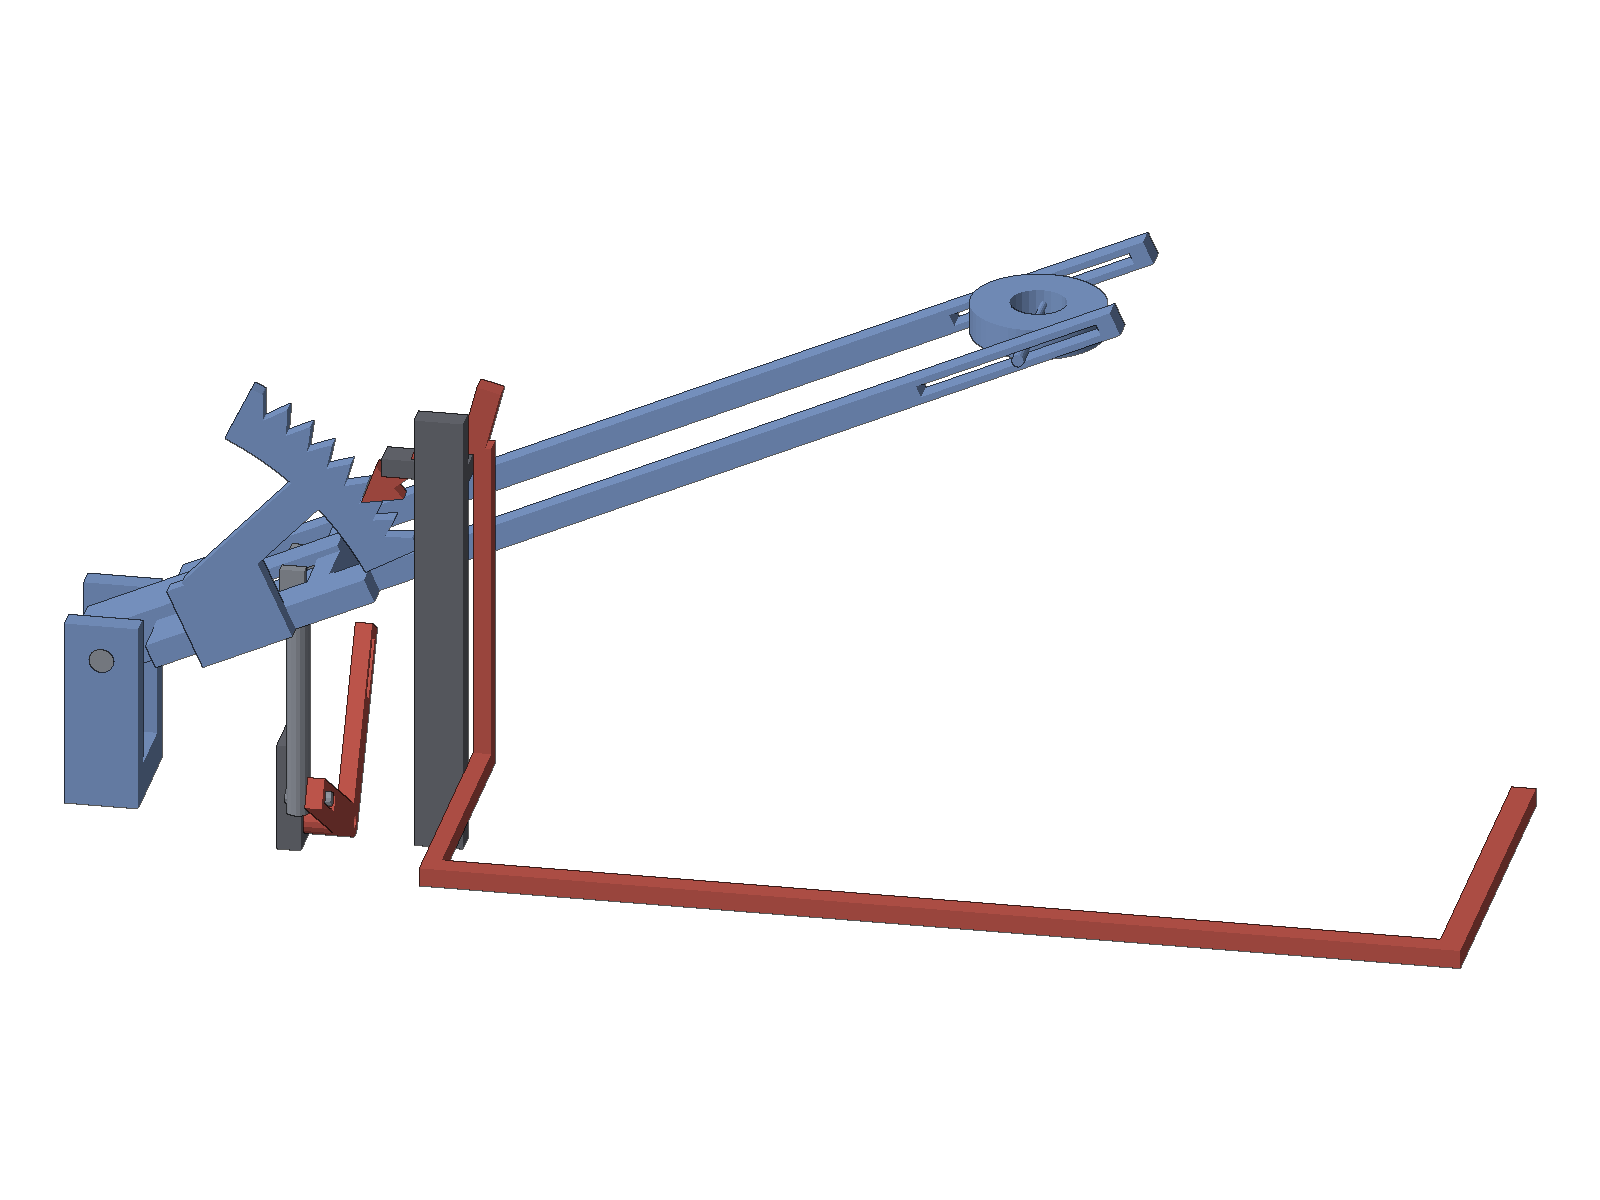
\includegraphics[width=0.5\linewidth]{gen/model/renders/row_detent.png}
\caption{Слева — молоток взведён: рычаг взвода на оси молотка, тяга от толкателя кулачка. Справа — фиксатор ряда: клин введён в гребёнку на вилке подъёма (ряд 5), тяга идёт от тяги фиксатора позиции.}
\label{fig:hammerrow}
\end{figure}

\subsection{Фиксатор ряда}

Пятого кулачка нет: клин фиксатора ряда ведёт тяга фиксатора позиции через поперечную тягу перед челноком и угловой рычаг, ход клина 5~мм. Гребёнка — на вилке подъёма, на радиусе 60~мм от её оси; вырезы с раствором 60° стоят там, где оказывается гребёнка, когда в строке нужный ряд: шаг от \mrdpmin\ до \mrdpmax~мм, захват — \mrdhub~мм хода ступицы, то есть почти полряда. Модель проверяет, что клин входит в вырез без натяга во всех восьми рядах и упирается в гребёнку между ними.

\subsection{Вибратор ленты}

Лента в покое опущена на \mribdrop~мм под строку (\S\ref{sec:vis}). Вилка из жести на ползуне под челноком поднимает её на время удара. С редакции 0.9.1 у ленты свой, пятый кулачок: толкатель с роликом поднимает тягу вибратора на 10~мм с 75° по 155°, держит до 175° и опускает к 255°; длинные склоны держат угол давления кулачка ниже 45°. Тяга проходит рядом с размахом приводной качалки дерева поворота, а тяга фиксаторов перешагивает её мостиком на высоте 138~мм. Масса подвижной части около 6~г, сила 0,6~Н, на знак это 6~мкДж — на энергию цикла не влияет.

\subsection{Блокировка клавиатуры}

Под рычагами лежит запорная гребёнка — стальная полоса 2~мм с прорезью 3,4~мм под каждый рычаг. В покое прорези стоят против рычагов, и любой рычаг проходит. Когда клавиша прошла 15,5~мм, рамка R или О спускает цикл, и на время оборота (с 5° по 345°) кулачок через тягу сдвигает гребёнку вдоль клавиатуры на \mlockshift~мм. Под язычком каждого поднятого рычага теперь стоит зуб (\mlocktooth~мм), и нажать его нельзя; нажатый рычаг держится в своей прорези шейкой толщиной \mlockneck~мм и не может подняться до конца оборота. Рычаг, нажатый во время цикла, упирается в зуб, пройдя у гребёнки 0,5~мм (около 1~мм хода клавиши, тогда как полный ход рычага у гребёнки — от 8 до 11,6~мм). Плавники рычагов проходят через шариковую дорожку из шариков 4,75~мм: в ней есть место ровно для одного плавника, поэтому две клавиши одновременно нажать нельзя.

\begin{figure}[H]
\centering
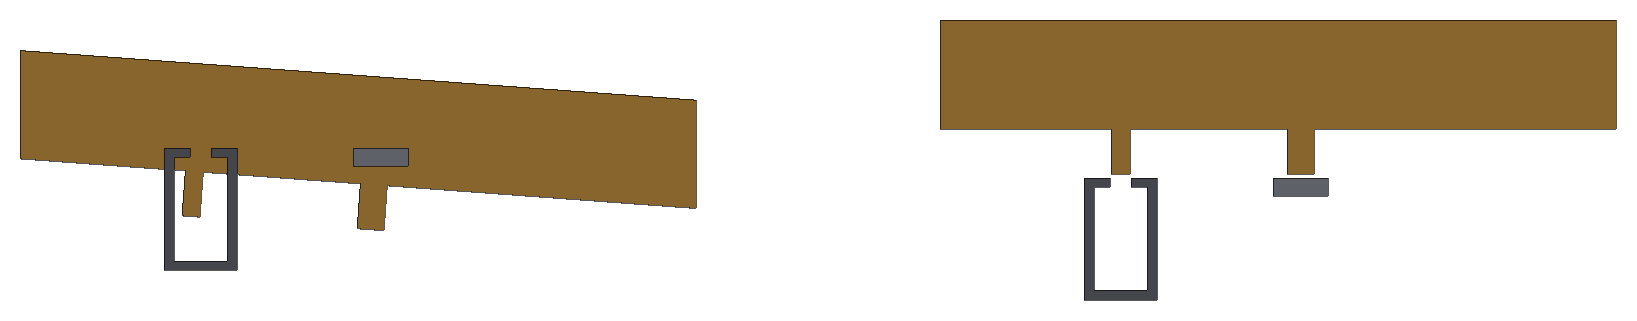
\includegraphics[width=0.9\linewidth]{gen/model/renders/lock.png}
\caption{Блокировка, разрез вдоль рычагов во время цикла (перед машинки справа). Слева — нажатый рычаг: его плавник вошёл в шариковую дорожку (тёмный жёлоб), а гребёнка (серый брусок) стоит в шейке рычага, так что подняться он не может до конца цикла. Справа — соседний рычаг: под его язычком стоит зуб сдвинутой гребёнки, нажать его нельзя.}
\label{fig:lock}
\end{figure}

\subsection{Ошибки редакции 0.7, найденные моделью}

Раньше движущиеся детали проверялись только с неподвижными; теперь каждая пара деталей из разных групп движения проверяется во всех состояниях. Это нашло ошибки, которые прежняя проверка пропускала:
\begin{itemize}
  \item каретка ленты поворота задевала фланец шкива на крайних позициях — направляющая перевёрнута, лента подходит с другой стороны;
  \item вилка подъёма была построена с неверной кинематикой: угол не соответствовал подъёму ступицы — теперь вилка на кулисах, угол $\arctan(\text{подъём}/150)$;
  \item боковины рамок проходили сквозь соседние рамки — они разведены по дорожкам;
  \item площадки толкателей кулачков перекрывались — каждому толкателю своя дорожка с пальцем;
  \item профиль кулачка молотка не совпадал с тем, что считал расчёт двигателя, — теперь оба берут взвод и спуск из одного описания цикла;
  \item в тексте оставалась фраза о подъёме челнока регистром на два ряда, хотя с редакции 0.6 регистр — разряд l4.
\end{itemize}
Кроме того, сборка документа повторяется теперь целиком одной командой \code{make} — от шрифта до PDF, STL и страницы; в редакции 0.7 часть промежуточных файлов собиралась вручную, а устаревший расчёт динамики падал с ошибкой и не входил в сборку.

\subsection{Упоры печатающего узла}
\label{sec:stops}

\paragraph{Нулевой упор и возврат.} В покое плита узла прижата пружиной растяжения (около 1~Н) к винту М3 в колодке на переднем брусе. Винт с контргайкой выставляет нулевое положение узла один раз: он переносит посадку всех знаков одинаково.

\paragraph{Упоры $b$ и $c$ — ступени на секторах.} Отдельных упоров нет: упором служит сам сектор памяти. На секторах B и C со стороны задней кромки сделана лесенка: ступень для значения $k$ стоит на радиусе $R_k = 33 - (8 + k)\,u$ мм под углом $-\theta_k$, где $\theta_k$ — угол, на который повторитель поворачивает сектор при ходе рамки $k$~мм. Когда сектор держит значение $k$, его ступень оказывается ровно против щупа на высоте оси секторов, и щуп, пройдя $(8 + k)\,u$, упирается в неё. Сила щупа направлена по радиусу, через ось, поэтому сектор она не поворачивает и собачку не нагружает. Проверка на модели: при каждом значении $k$ щуп за 0,15~мм до расчётного отвода свободен, а через 0,25~мм после — входит в ступень.

\begin{center}\small
\begin{tabular}{@{}ccccccc@{}}
\toprule
& \multicolumn{2}{c}{отвод} & \multicolumn{2}{c}{сектор B} & \multicolumn{2}{c}{сектор C} \\
\cmidrule(lr){2-3}\cmidrule(lr){4-5}\cmidrule(lr){6-7}
$k$ & $u$ & мм & $\theta_k$, ° & $R_k$, мм & $\theta_k$, ° & $R_k$, мм \\
\midrule
\tabinput{gen/tab_stops.tex}
\bottomrule
\end{tabular}
\end{center}

\paragraph{Передача от узла к щупу.} Под плитой узла закреплён щуп — стальная полоса 4$\times$4~мм, идущая вдоль правого края вперёд. Его торец давит на ролик синусного углового рычага (плечи по 15~мм, вертикальная ось на кронштейне от щеки двигателя); второй ролик рычага двигает каретку щупа по направляющей вдоль $-Y$. Оба ролика лежат на плоских площадках под прямым углом друг к другу, так что каретка проходит ровно столько, сколько узел, при повороте рычага до \mstopbc°. На каретке — ползунок со щупом: вертикальный палец, торец которого стоит на высоте оси секторов в 33~мм от неё.

\paragraph{Выбор B или C.} Плоскости секторов B и C разнесены на 5~мм. Ползунок щупа по умолчанию стоит в плоскости B; рамка N через рычаг с роликом на своей балке (плечи 14,5 и 62,5~мм) сдвигает его в плоскость C за первые \mstopnt~мм своего хода, после чего рычаг ложится на упор, а балка идёт дальше одна. В покое щуп отстоит от самой высокой ступени на \mstopfree~мм, и к моменту, когда сдвиг закончен, узел успевает отойти лишь на \mstopslideN~мм, — щуп не может зацепить чужую ступень.

\paragraph{Тяга от рамки О.} Рамка О ведёт узел слева: повторитель О сидит на продолжении оси левого повторителя W, его плечо 12~мм вниз толкает тягу A вперёд (до \mopush~мм при ходе рамки 12~мм; дальше рычаг ложится на упор). Тяга A состоит из двух половин с пружиной сжатия между ними (поджатие 1,5~Н, до \mstopFmax~Н), за клавишами она качает качалку 33/34~мм на стойке запорной гребёнки, та тянет тягу B над рычагами, а угловой рычаг 12/12~мм с роликом толкает упор, привёрнутый к плите узла снизу. Узел идёт за тягой, пока щуп не упрётся в ступень; остаток хода рамки забирает пружина. Наибольшая добавка к усилию на выступе О — около \mstopkey~Н; её стоит сравнить с замерами стенда Э2.

\begin{figure}[H]
\centering
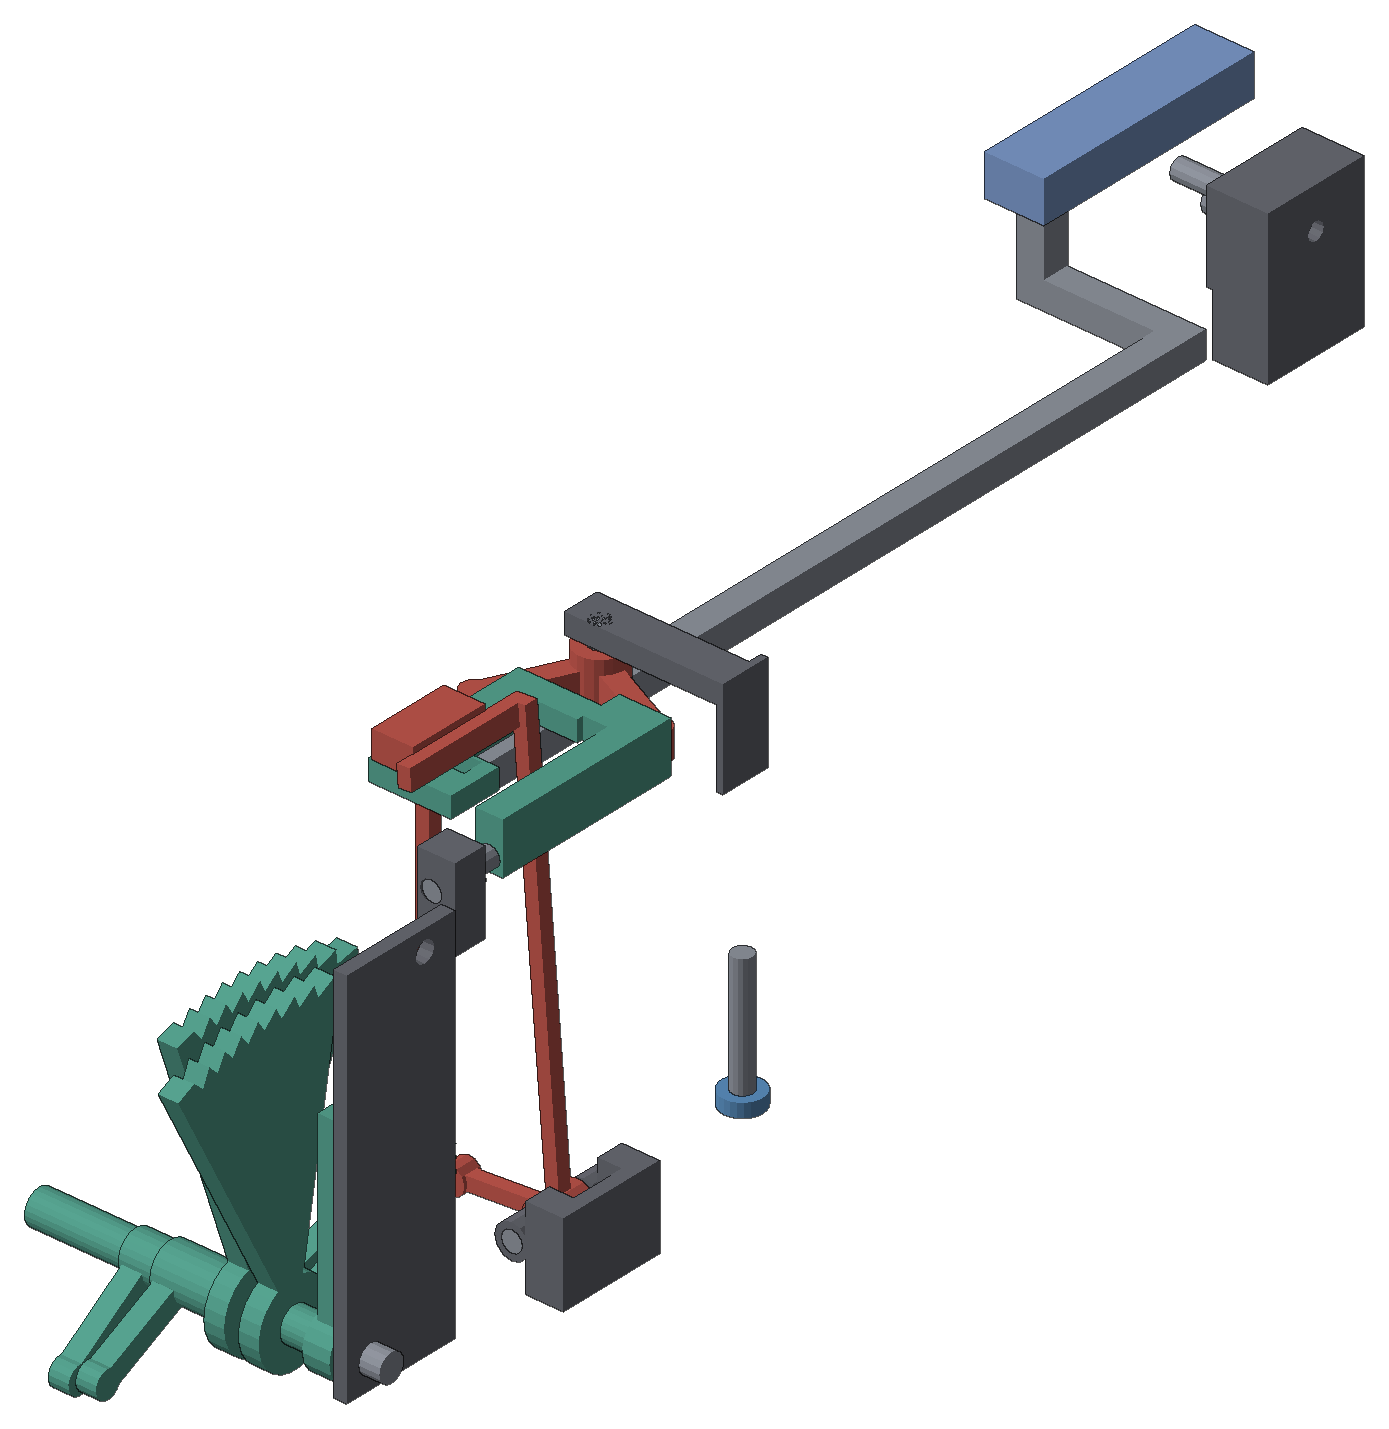
\includegraphics[width=0.49\linewidth]{gen/model/renders/stops.png}\hfill
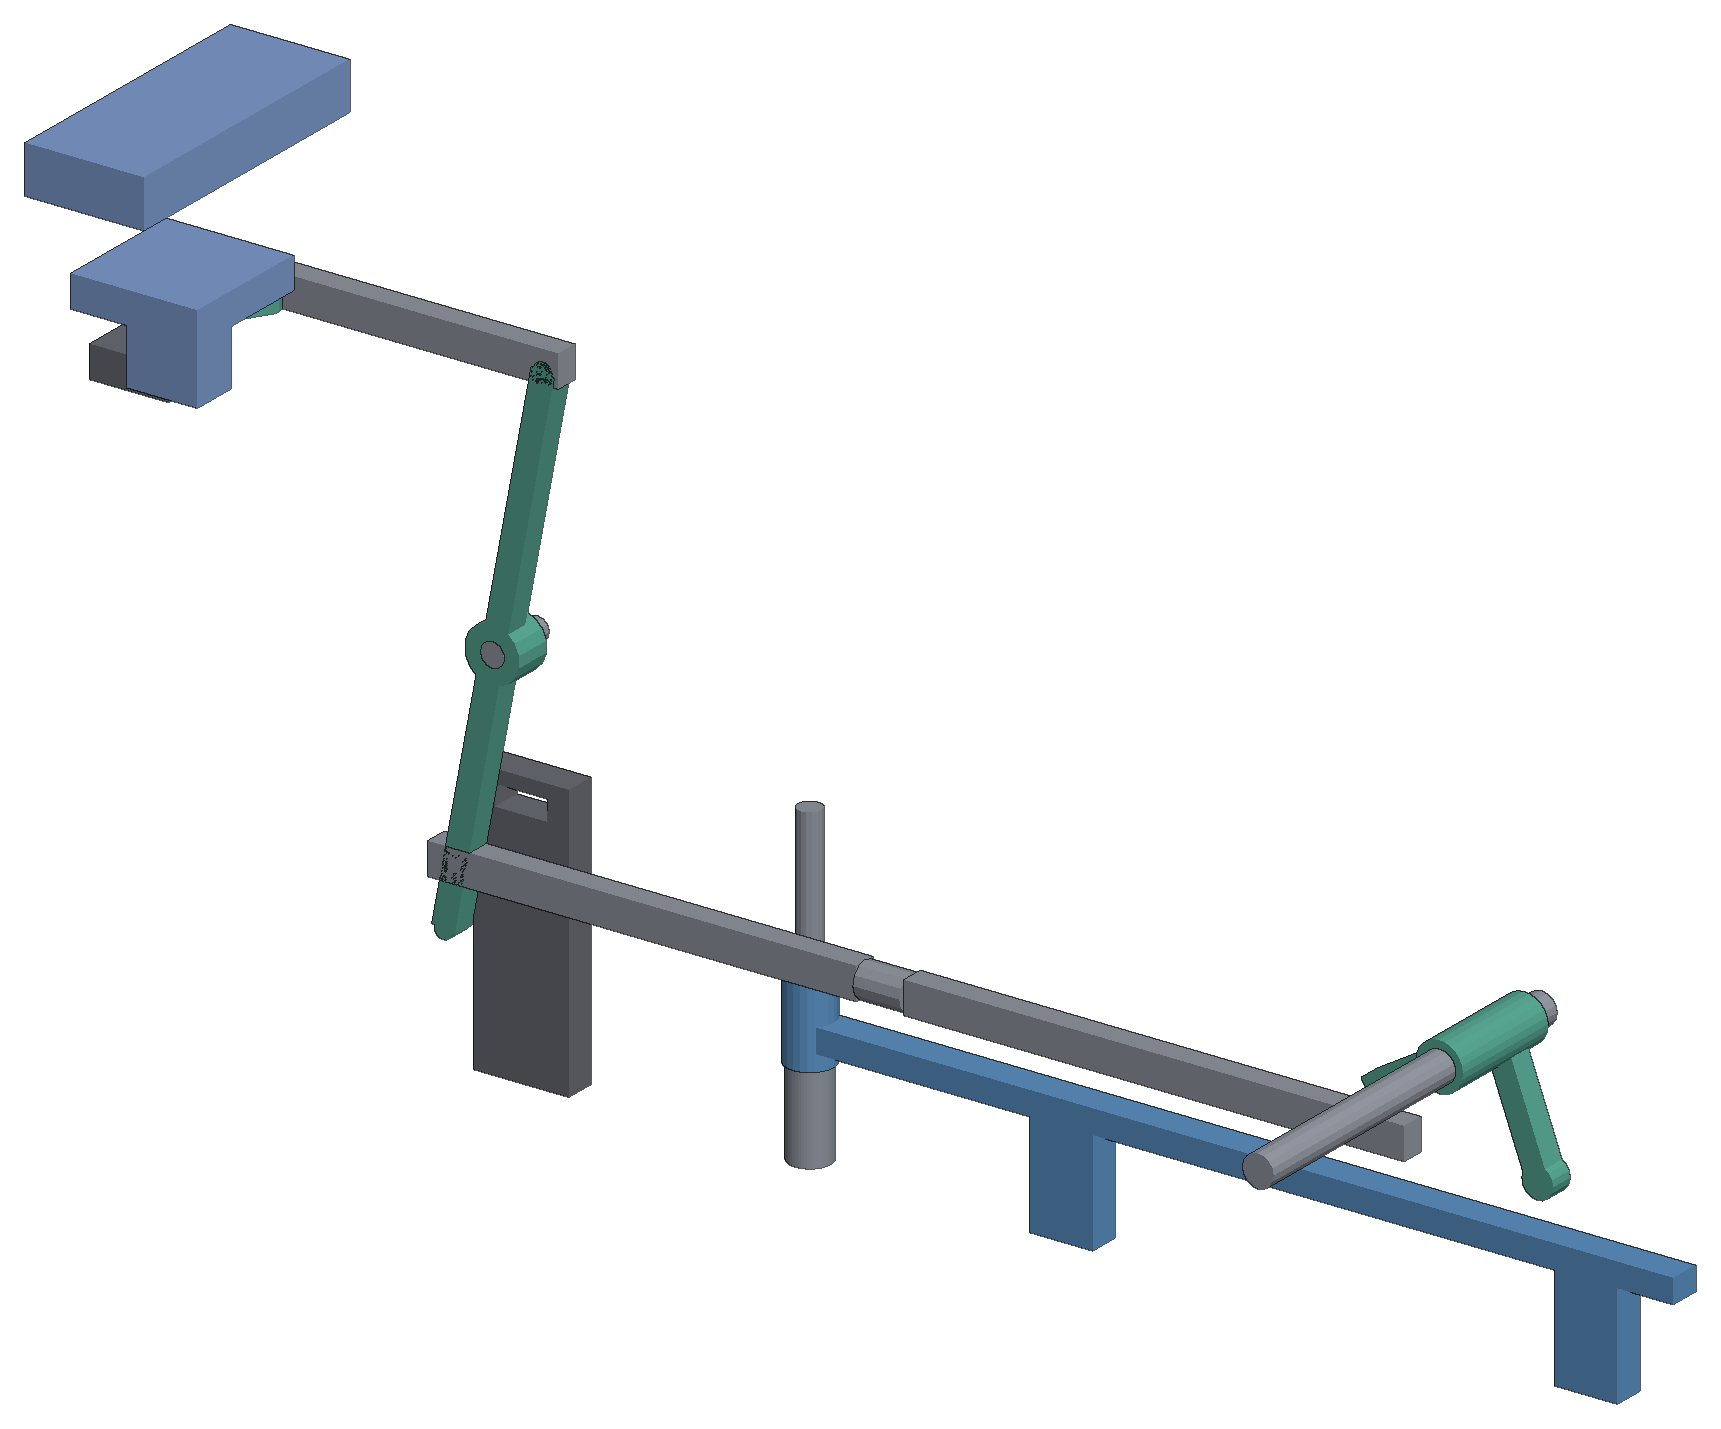
\includegraphics[width=0.49\linewidth]{gen/model/renders/olink.png}
\caption{Слева — упоры для подстрочного знака при памяти $c = 4$: щуп на плите узла, синусный рычаг, каретка щупа, ползунок, сдвинутый рычагом N в плоскость сектора C, ступени на секторах; сзади — нулевой упор с винтом. Справа — тяга от рамки О: повторитель О, тяга A с пружиной, качалка за клавишами, тяга B, угловой рычаг и упор на плите узла.}
\label{fig:stops}
\end{figure}

\subsection{Пружины рамок}

Каждая рамка стоит на двух пружинах сжатия 5,2$\times$0,5~мм, надетых на её задние направляющие между полосой основания и гильзой боковины. Пружины поднимают рамку в покой и дают силу из таблицы мерных рамок; при ходе 16~мм они сжимаются на половину длины.

\subsection{Спуск, забой и «назад на литеру»}
\label{sec:back}

В редакции 0.9.1 спуск построен в модели заново (\code{tools/model/escape.py}) вместе с забоем, «назад на литеру» и рычажком $\pm u$. Колесо идёт вперёд по часовой стрелке (если смотреть сверху): так его поворачивает рейка под шестернёй, когда каретка уходит влево. У каждого зуба радиальный торец, обращённый против хода, и скос, поднимающийся от впадины (R~18~мм) к вершине (R~20,5~мм).

\begin{figure}[H]
\centering
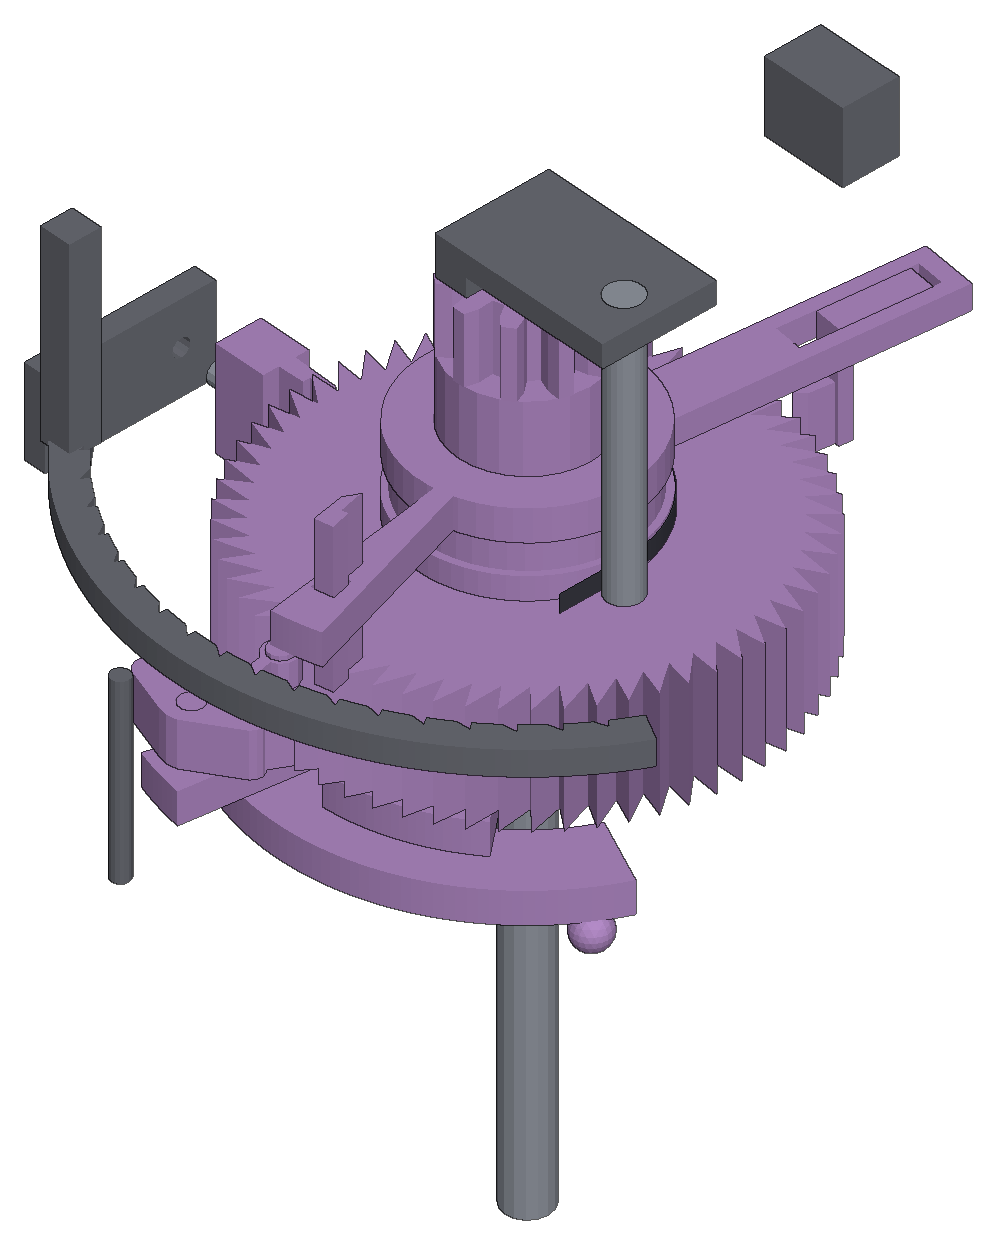
\includegraphics[width=0.49\linewidth]{gen/model/renders/escapement.png}\hfill
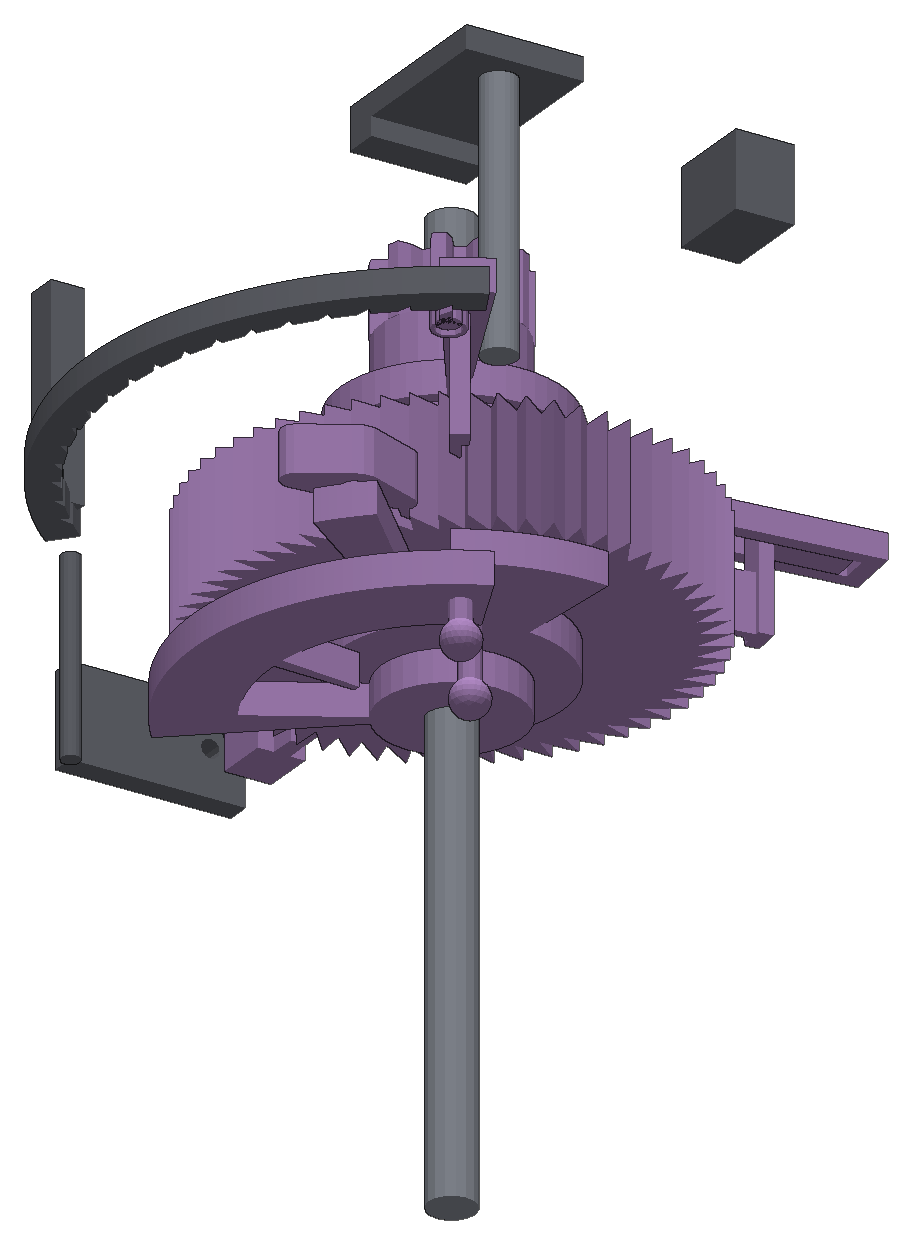
\includegraphics[width=0.49\linewidth]{gen/model/renders/escapement_back.png}
\caption{Спуск в модели. Слева — покой, вид сверху спереди (память M держит ширину 8): колесо в два этажа с шестернёй, над ним барабан и рычаг упора U с пальцем-ползуном, выше — рычаг памяти M с клином и собачкой в неподвижном храповом секторе, сзади — собачка Д в направляющей. Справа — «назад на литеру» в конце хода, вид снизу: рычаг B повернул колесо назад, под ним рычаг забоя K; на обоих — шаровые пальцы тяг; клин M сцеплён с колесом.}
\label{fig:escapement}
\end{figure}

\begin{itemize}
  \item \textbf{Колесо в два этажа.} Колесо толщиной 10~мм: в нижний этаж входят собачка B и собачка Д, в верхний — палец U, клин M и снова Д. Шестерня $z = 10$ и колесо — одна деталь.
  \item \textbf{Собачка Д} — ползун в направляющей за колесом; её клин повторяет впадину и касается торца зуба. Когда колесо идёт назад, Д поднимается по скосам и падает в следующую впадину.
  \item \textbf{Упор U} — барабан R~9,55~мм над колесом; стальная лента от тяги X охватывает его снизу, поэтому 1~мм хода тяги — ровно 6°, один зуб. Тяга X идёт под барабаном и тянет к $-X$, и барабан поворачивается вперёд вместе с колесом. На рычаге U — палец-ползун: в покое он выведен из зубьев на 3~мм, перед спуском входит; модель проверяет, что во всех положениях от 4 до 17 зубьев он стоит у торца без зазора.
  \item \textbf{Рычажок $\pm u$} стоит под осью углового рычага тяги W: эксцентрик 1~мм в трёх положениях сдвигает тягу X на одну единицу, и следующая литера проходит $w-1$, $w$ или $w+1$ единиц.
  \item \textbf{Рычаг B} — под колесом, на оси спуска. Собачка B в покое лежит хвостом на штифте-щитке и стоит над вершинами зубьев. Первые \mbdrop° поворота B (против часовой) хвост сходит со щитка, собачка падает, на \mbcatch° встречает торец и дальше ведёт колесо назад. Шаровой палец B на радиусе 13~мм тянет тяга «назад на литеру».
  \item \textbf{Забой.} Свой рычаг K на той же оси толкает B пальцем под шаровой палец B; тяга забоя поворачивает K на \mbkspdeg°: после \mbcatch° свободного хода колесо уходит назад на 1,2 зуба, Д падает за следующий торец, и пружина каретки возвращает колесо на Д — ровно 1\,u назад. Когда работает «назад на литеру», B уходит от пальца K, и тяга забоя стоит на месте.
  \item \textbf{Память ширины M} — над барабаном U. На M клин сцепления, который повторяет впадину с люфтом \mmplay° со стороны скоса, и собачка в неподвижном храповом секторе с шагом 6°. При спуске клин входит в зубья, и M идёт вперёд вместе с колесом ровно на $w$ зубьев; собачка держит его там. Когда U снова уходит от нуля, собачка отпускается, и пружина M возвращает его на упор нуля.
  \item \textbf{«Назад на литеру».} Тяга этой клавиши поворачивает B; одновременно её качалка вводит клин M и отпускает собачку M. Колесо уходит назад вместе с M, пока M не встанет на свой упор нуля, — то есть на $w$ зубьев и \mmplay° люфта клина; на этих \mmplay° Д падает в зуб, и колесо возвращается на неё. Если затем ударить ту же литеру через корректирующую ленту, она ляжет на прежнее место.
  \item \textbf{Привод от клавиш.} В торцах хвостов рычагов забоя и «назад на литеру» — пальцы вдоль $Y$, они ходят в пазах входных плеч двух качалок на осях вдоль $Y$ за хвостами (стенка качалок у правого края клавиатуры). Нижнее плечо качалки забоя (9~мм) и верхнее качалки «назад на литеру» (40~мм) тянут тяги с шаровыми наконечниками к пальцам K и B. При полном ходе клавиши тяга забоя проходит \mbksppull~мм при нужных \mbkspneed, тяга «назад на литеру» — \mbackpull~мм при нужных \mbackneed~мм для $w = 16$; остаток забирает пружина в тяге, у тяги забоя есть ещё упорная втулка.
\end{itemize}

\paragraph{Что не построено.} Подвижные детали, которые только включают и выключают механизм, даны в модели положениями, а не деталями: колодка на U, отпускающая собачку M, ввод пальца U и клина M перед спуском, ввод клина M качалкой «назад на литеру». Пружины даны размерами и силами, их жёсткость нужно подобрать по замерам стенда Э2.

%=====================================================================
\section{Ход клавиши}
\label{sec:budget}

\subsection{Поля и указатель точки печати}
\label{sec:margins}

\paragraph{Поля.} Как у обычной машинки, начало и конец строки ставятся упорами, а не меткой на бумаге. На рейке каретки (зубья через 3,175~мм — это 6\,u) сидят два упора полей — печатные защёлки, которые охватывают рейку сзади и встают на любой зуб; над рейкой, на кронштейне спуска, неподвижный упор полей стоит между ними. Возвращаясь, каретка идёт вправо, пока упор левого поля не встанет на левую грань упора полей, — здесь начинается строка. При наборе каретка уходит влево, и в конце строки на правую грань приходит упор правого поля: дальше каретка не подаётся. Поля ставятся с шагом 6\,u; без переставленных упоров строка — полная, 170~мм. Модель проверяет касание упоров с упором полей в начале и в конце строки (\S\ref{sec:contacts}) и ход каретки по всей строке с ними (\S\ref{sec:checks}); на странице модели поля задаются в зубьях рейки, перевод строки возвращает каретку к левому полю. \paragraph{Освобождение каретки.} Слева на передней раме стоит клавиша освобождения каретки — рычажок 14/14~мм на оси. Нажатая на 3~мм, она тянет боуденовский трос к хвосту держащей собачки спуска; собачка выходит из колеса (кончик — в 0,85~мм от зубьев), палец U в покое и так выведен, и каретку можно сдвинуть рукой в любую сторону — к нужному месту строки или чтобы начать печать не от поля. Когда клавиша отпущена, пружина собачки вводит её между зубьями: каретка встаёт на целую единицу (зуб колеса — 1\,u). Упоры полей при этом по-прежнему ограничивают ход. Модель проверяет ход собачки, клавиши и каретки с выведенной собачкой в начале, середине и конце строки (\S\ref{sec:checks}); на странице модели каретка сдвигается так кнопками на заданное число единиц.

\paragraph{Чего нет.} Звонок перед концом строки и запор клавиатуры на правом поле пока не построены: у обычной машинки правый упор за 6--8 знаков до конца бьёт по молоточку звонка, а на самом упоре запирает клавиши; здесь клавиша на правом поле напечатает знак поверх предыдущего. Вертикально лист выставляется валиком.

\paragraph{Указатель точки печати.} У обычной машинки точку печати показывают метки на прижимной планке у самого листа. Здесь перед листом в точке печати стоит челнок: на расстоянии до 10~мм от оси удара его лицо почти касается листа, а выше и ниже строки ходят его ряды. Свободное место на оси удара есть только внутри кольца, над головкой чтения. Туда поставлена проволока 0,8~мм с красной бусиной 1,6~мм — на оси молотка, в 27,5~мм перед листом. С обычной посадки (глаз в 720~мм перед машинкой и на 460~мм над столом) бусина видна поверх челнока и стоит на строке на 1,9~мм выше линии шрифта — там, где ляжет левый край следующей литеры. Указатель сидит на U-раме, поэтому для мёртвого знака он отходит вместе с молотком и показывает, куда встанет знак. Цена расстояния до листа — параллакс: если глаз выше или ниже на 80~мм, бусина смещается на строке на 3--4~мм по высоте, при сдвиге головы вбок на 100~мм — примерно на 4~мм вдоль строки. Это прицел для глаза над клавиатурой, а не метка на бумаге.

\subsection{Бюджет хода}

До редакции 0.9.3 ход клавиши задавал и код: выступ W самой широкой литеры начинал вести свою планку уже на 4~мм, и сброс R должен был закончиться раньше. Таблица ниже — тот выбор $T_p$ и $k$, сохранённый для истории.

\begin{center}\small
\begin{tabular}{@{}rrrrrrrc@{}}
\toprule
& & & \multicolumn{3}{c}{наименьший зазор, мм} & & \\
\cmidrule(lr){4-6}
$T_p$, мм & клавиша, мм & $k$, мм/u & W & B & C & $k/2$, мм & сброс успел \\
\midrule
\tabinput{gen/tab_budget_fdm.tex}
\bottomrule
\end{tabular}
\end{center}

\paragraph{С редакции 0.10.} Замер ушёл в цикл (\S\ref{sec:read}); ступень $k = 1{,}0$~мм/u осталась, но это теперь глубина зубца гребёнки, а не зазор выступа. Ход клавиши 16~мм пока сохранён: на нём держатся сброс R (первые 3,5~мм), спуск цикла на 15,5~мм, ход рамки О с тягой отвода и храповики полного хода. Укоротить его можно, но для этого надо пересчитать тягу О и блокировки; это задача следующей редакции.

\subsection{Порядок действий}

\begin{figure}[h]
\centering
\begin{tikzpicture}[x=5.4mm,y=1mm]
\draw[ink!50,->] (0,0) -- (18.6,0);
\foreach \x in {0,2,...,16} {\draw[ink!50] (\x,0) -- (\x,-1.5) node[lbl,below]{\x};}
\node[lbl,anchor=north] at (8,-5) {ход кодовой пластины и клавиши, мм};
\node[lbl,anchor=north] at (17.6,-5) {отпуск.};
\def\row#1#2{\node[lbl,anchor=east] at (-0.2,#1) {#2};}
\node[lbl,anchor=west,font=\sffamily\footnotesize\bfseries] at (0,74) {мёртвый знак};
\row{68}{отвод ползуна (О), тяга} \fill[sledA!40] (0,66) rectangle (10,70);
\row{61}{выбор: толкатель и планки} \fill[accent!30] (0.5,59) rectangle (9,63);
\row{54}{спуск цикла} \fill[axisred] (15.7,52) rectangle (16,56);
\row{47}{цикл; затем возврат ползуна} \fill[sledA!25] (16.1,45) rectangle (18.2,49);
\node[lbl,anchor=west,font=\sffamily\footnotesize\bfseries] at (0,40) {продвигающая литера};
\row{34}{сброс памяти (R)} \fill[accent!35] (0,32) rectangle (3.5,36);
\row{27}{код W, B, C — с челнока, в цикле} \fill[sledB!15] (16.1,25) rectangle (18.2,29);
\row{20}{выбор: толкатель и планки} \fill[accent!30] (0.5,18) rectangle (9,22);
\row{13}{спуск цикла} \fill[axisred] (15.7,11) rectangle (16,15);
\row{6}{цикл; затем подача $w$} \fill[axisblue!45] (16.1,4) rectangle (18.2,8);
\end{tikzpicture}
\caption{Порядок действий по ходу пластины ($T_p = 16$~мм). С ред. 0.10 клавиша только сбрасывает память, выбирает литеру и в самом низу хода спускает цикловой вал; код W, B, C щупы читают с челнока уже в цикле, после фиксации (рис.~\ref{fig:cycle}), там же поворот челнока, удар и подача.}
\label{fig:stroke}
\end{figure}

\subsection{Допуск на код}
\label{sec:gaptol}

С редакции 0.10 кодом служит не зазор выступа, а ход щупа до зубца гребёнки; рассуждение то же. Фиксатор доводит значение до ближайшей единицы, поэтому ошибка зазора меньше половины ступени (0,5~мм) не вредит. Если ошибку зазора (настройка выступа плюс зазоры в шарнирах планки) считать нормальной со стандартным отклонением $\sigma$, вероятность промаха на одном замере — $2\,(1-\Phi(0{,}5/\sigma))$.

\begin{center}\small
\begin{tabular}{@{}rrrrr@{}}
\toprule
$\sigma$, мм & $\pm3\sigma$, мм & запас $0{,}5/\sigma$ & промах на замер & промахов на страницу \\
\midrule
\tabinput{gen/tab_gap_fdm.tex}
\bottomrule
\end{tabular}
\end{center}

\noindent{\small Страница — около 1500 продвигающих литер по три замера (допущение).}

\paragraph{Требование.} $\sigma \le 0{,}08$~мм (допуск около $\pm 0{,}25$~мм) — практически ни одного промаха; при $\sigma = 0{,}1$~мм промах бывает примерно раз на 400 страниц, при 0,15~мм — несколько на странице. Печатный выступ таких допусков не держит, а винт, выставленный щупом, держит; поэтому выступы регулируемые. Люфты в шарнирах планок закрываются стальными осями в развёрнутых отверстиях.

\paragraph{Для гребёнок (ред. 0.10).} Ошибку хода щупа складывают: положение торца зубца на гребёнке (печать на ребре, в плоскости стола: около 0,04~мм после калибровки шага, \S\ref{sec:fdm}), посадка гребёнки на кольце (штифты в развёрнутых отверстиях, прижим к поясу — около 0,03~мм), биение кольца на валу, люфт щупа в пазу, удлинение и трение троса и посадка ползунка — по оценке ещё 0,04~мм. Вместе это около 0,07~мм, у самой границы требования. Постоянная часть ошибки (усадка кольца, длина троса) снимается винтом нуля каждого канала один раз по контрольному тексту; печатная гребёнка, в отличие от выступа на пластине, допуск держит, потому что её мерная поверхность лежит в плоскости стола. Это нужно подтвердить на стенде Э2 замером ходов щупов по всем клеткам.

%=====================================================================
\section{Силы и энергия}
\label{sec:forces}

Челнок и молоток приводит цикл, а с редакции 0.10 и чтение кода (\S\ref{sec:read}), поэтому продвигающая клавиша выполняет только сброс, выбор и спуск цикла. Работа считается на ходе пластины, он же ход клавиши; для сравнения в таблице оставлены строки замера, которые клавиша делала до 0.9.3 (худший случай $w = 16$, $b = 8$, $c = 9$):

\begin{center}\small
\begin{tabular}{@{}lrrr@{}}
\toprule
Работа на ходу продвигающей клавиши & сила, Н & путь, мм & работа, мДж \\
\midrule
планка R (сброс) & 0,3 & 3,5 & 1,05 \\
толкатель выбора и планки & 0,5 & 3,0 & 1,50 \\
спуск цикла, блокировки, трение & & & 1,00 \\
\midrule
\textbf{итого в 0.10} & & & \textbf{3,6} \\
\midrule
\textit{до 0.9.3 ещё: планка W ($w - 4 = 12$)} & 0,3 & 12,0 & 3,60 \\
\textit{планка B} & 0,3 & 8,0 & 2,40 \\
\textit{планка C} & 0,3 & 9,0 & 2,70 \\
\textit{итого в 0.9.3} & & & \textit{12,3} \\
\bottomrule
\end{tabular}
\end{center}

На ходе клавиши 16~мм это в среднем 0,22~Н, около 23~гс (было 0,77~Н, около 80~гс). Мёртвая клавиша не изменилась: отвод ползуна на 9~мм пружинной тягой 1,2~Н на первых 10~мм хода (12~мДж), выбор (1,5~мДж) и спуск (1~мДж) — около 14,5~мДж, в среднем около 90~гс. Теперь мёртвые клавиши вчетверо тяжелее буквенных (14,5 против 3,6~мДж); чтобы рука не чувствовала разницы, буквенным клавишам стоит добавить возвратную пружину (около 0,3~Н) или облегчить тягу О. Энергию на челнок, молоток и чтение кода даёт заводная пружина (\S\ref{sec:motor}).

\paragraph{Чего не хватает.} Силы пружин и трение — допущения. Их заменят замеры на стенде этапа Э2; пружины планок можно частично уравновесить встречными.

%=====================================================================
\section{Литеры}

\begin{figure}[H]
\centering
\setlength\tgem{26mm}
\begin{tikzpicture}[x=\tgu,y=\tgu]
\draw[slug] (-60,-400) rectangle (685.0,820);
\fill[cellfill] (0,-330) rectangle (625.0,740);
\node[anchor=base west,inner sep=0pt,outer sep=0pt] at (9.5,0.0) {\TG{54}};
\draw[axisT,thin,draw=ink!35] (312.5,-330) -- (312.5,760);
\draw[ppoint] (0,-470) -- (0,900);
\draw[dim] (0,-540) -- (625.0,-540);
\node[lbl,anchor=north] at (312.5,-570) {$w{=}10$};
\node[lbl,anchor=north] at (312.5,-700) {$b{=}5$, $c{=}4$};
\node[lbl,anchor=south] at (312.5,930) {tinco};
\draw[slug] (825.0,-400) rectangle (1945.0,820);
\fill[cellfill] (885.0,-330) rectangle (1885.0,740);
\node[anchor=base west,inner sep=0pt,outer sep=0pt] at (903.0,0.0) {\TG{58}};
\draw[axisT,thin,draw=ink!35] (1385.0,-330) -- (1385.0,760);
\draw[ppoint] (885.0,-470) -- (885.0,900);
\draw[dim] (885.0,-540) -- (1885.0,-540);
\node[lbl,anchor=north] at (1385.0,-570) {$w{=}16$};
\node[lbl,anchor=north] at (1385.0,-700) {$b{=}8$, $c{=}7$};
\node[lbl,anchor=south] at (1385.0,930) {ando};
\draw[slug] (2085.0,-400) rectangle (2830.0,820);
\fill[cellfill] (2145.0,-330) rectangle (2770.0,740);
\node[anchor=base west,inner sep=0pt,outer sep=0pt] at (2162.0,0.0) {\TG{64}};
\draw[axisT,thin,draw=ink!35] (2395.0,-330) -- (2395.0,760);
\draw[ppoint] (2145.0,-470) -- (2145.0,900);
\draw[dim] (2145.0,-540) -- (2770.0,-540);
\node[lbl,anchor=north] at (2457.5,-570) {$w{=}10$};
\node[lbl,anchor=north] at (2457.5,-700) {$b{=}6$, $c{=}5$};
\node[lbl,anchor=south] at (2457.5,930) {harma};
\draw[slug] (2970.0,-400) rectangle (3652.5,820);
\fill[cellfill] (3030.0,-330) rectangle (3592.5,740);
\node[anchor=base west,inner sep=0pt,outer sep=0pt] at (3015.5,0.0) {\TG{94}};
\draw[axisT,thin,draw=ink!35] (3467.5,-330) -- (3467.5,760);
\draw[ppoint] (3030.0,-470) -- (3030.0,900);
\draw[dim] (3030.0,-540) -- (3592.5,-540);
\node[lbl,anchor=north] at (3311.25,-570) {$w{=}9$};
\node[lbl,anchor=north] at (3311.25,-700) {$b{=}2$, $c{=}5$};
\node[lbl,anchor=south] at (3311.25,930) {hyarmen};
\draw[slug] (3792.5,-400) rectangle (4162.5,820);
\fill[cellfill] (3852.5,-330) rectangle (4102.5,740);
\node[anchor=base west,inner sep=0pt,outer sep=0pt] at (3852.5,0.0) {\TG{100}};
\draw[axisT,thin,draw=ink!35] (3977.5,-330) -- (3977.5,760);
\draw[ppoint] (3852.5,-470) -- (3852.5,900);
\draw[dim] (3852.5,-540) -- (4102.5,-540);
\node[lbl,anchor=north] at (3977.5,-570) {$w{=}4$};
\node[lbl,anchor=north] at (3977.5,-700) {$b{=}2$, $c{=}2$};
\node[lbl,anchor=south] at (3977.5,930) {telco};
\draw[slug] (4302.5,-400) rectangle (4672.5,820);
\fill[cellfill] (4362.5,-330) rectangle (4612.5,740);
\node[anchor=base west,inner sep=0pt,outer sep=0pt] at (4359.5,0.0) {\TG{98}};
\node[anchor=base west,inner sep=0pt,outer sep=0pt] at (4374.5,0.0) {\TG{317}};
\draw[axisT,thin,draw=ink!35] (4487.5,-330) -- (4487.5,760);
\draw[ppoint] (4362.5,-470) -- (4362.5,900);
\draw[dim] (4362.5,-540) -- (4612.5,-540);
\node[lbl,anchor=north] at (4487.5,-570) {$w{=}4$};
\node[lbl,anchor=north] at (4487.5,-700) {$b{=}2$, $c{=}2$};
\node[lbl,anchor=south] at (4487.5,930) {ára+e};

\end{tikzpicture}
\caption{Продвигающие литеры (увеличено). Красная линия — ось молотка (левый край клетки), серая — ось техты. Под литерой её код.}
\end{figure}

\begin{figure}[H]
\centering
\setlength\tgem{24mm}
\begin{tikzpicture}[x=\tgu,y=\tgu]
\draw[slug,fill=sledA!12] (-60,-400) rectangle (480,820);
\node[anchor=base west,inner sep=0pt,outer sep=0pt] at (51.0,0.0) {\TG{311}};
\draw[ppoint] (210.0,-470) -- (210.0,900);
\node[lbl,anchor=north] at (210.0,-570) {отвод $b$};
\node[lbl,anchor=south] at (210.0,930) {a};
\draw[slug,fill=sledA!12] (620,-400) rectangle (1160,820);
\node[anchor=base west,inner sep=0pt,outer sep=0pt] at (777.0,0.0) {\TG{317}};
\draw[ppoint] (890.0,-470) -- (890.0,900);
\node[lbl,anchor=north] at (890.0,-570) {отвод $b$};
\node[lbl,anchor=south] at (890.0,930) {e};
\draw[slug,fill=sledA!12] (1300,-400) rectangle (2328,820);
\node[anchor=base west,inner sep=0pt,outer sep=0pt] at (1400.0,0.0) {\TG{362}};
\draw[ppoint] (1814.0,-470) -- (1814.0,900);
\node[lbl,anchor=north] at (1814.0,-570) {отвод $b$};
\node[lbl,anchor=south] at (1814.0,930) {нос. шир.};
\draw[slug,fill=sledB!12] (2468,-400) rectangle (3008,820);
\node[anchor=base west,inner sep=0pt,outer sep=0pt] at (2586.0,0.0) {\TG{314}};
\draw[ppoint] (2738.0,-470) -- (2738.0,900);
\node[lbl,anchor=north] at (2738.0,-570) {отвод $c$};
\node[lbl,anchor=south] at (2738.0,930) {y};
\draw[slug,fill=sledB!12] (3148,-400) rectangle (3836,820);
\node[anchor=base west,inner sep=0pt,outer sep=0pt] at (3248.0,0.0) {\TG{329}};
\draw[ppoint] (3492.0,-470) -- (3492.0,900);
\node[lbl,anchor=north] at (3492.0,-570) {отвод $c$};
\node[lbl,anchor=south] at (3492.0,930) {удв. узк.};
\draw[slug,fill=sledB!12] (3976,-400) rectangle (4564,820);
\node[anchor=base west,inner sep=0pt,outer sep=0pt] at (4137.0,0.0) {\TG{346}};
\draw[ppoint] (4270.0,-470) -- (4270.0,900);
\node[lbl,anchor=north] at (4270.0,-570) {отвод $c$};
\node[lbl,anchor=south] at (4270.0,930) {удв. lambe};

\end{tikzpicture}
\caption{Мёртвые знаки (увеличено). Якорь знака — на оси молотка; под знаком указано, на какую величину уходит узел.}
\end{figure}

Набор знаков тот же, что в ТПМ-1: один комплект гласных на все тенгвы, черта удвоения и носовая черта в узком и широком вариантах, особая черта для lambe и alda, литеры «ára + гласная».

%=====================================================================
\section{Раскладка}

\begin{figure}[H]
\centering
\begin{tikzpicture}[x=1mm,y=1mm]
\draw[key,fill=keyadv] (0.0,0.0) rectangle +(12.4,-14.0);
\node[keyleg] at (11.4,-1.2) {\texttt{1}};
\node[anchor=base,inner sep=0pt,keyup] at (3.9680000000000004,-4.6) {{\tgkeyU\symbol{"E07B}}};
\node[anchor=base,inner sep=0pt,keylo] at (7.4399999999999995,-10.9) {{\tgkeyL\symbol{"E071}}};
\draw[key,fill=keyadv] (13.700000000000001,0.0) rectangle +(12.4,-14.0);
\node[keyleg] at (25.1,-1.2) {\texttt{2}};
\node[anchor=base,inner sep=0pt,keyup] at (17.668000000000003,-4.6) {{\tgkeyU\symbol{"E060}}};
\node[anchor=base,inner sep=0pt,keylo] at (21.14,-10.9) {{\tgkeyL\symbol{"E072}}};
\draw[key,fill=keyadv] (27.400000000000002,0.0) rectangle +(12.4,-14.0);
\node[keyleg] at (38.800000000000004,-1.2) {\texttt{3}};
\node[anchor=base,inner sep=0pt,keyup] at (31.368000000000002,-4.6) {{\tgkeyU\symbol{"E061}}};
\node[anchor=base,inner sep=0pt,keylo] at (34.84,-10.9) {{\tgkeyL\symbol{"E073}}};
\draw[key,fill=keyadv] (41.1,0.0) rectangle +(12.4,-14.0);
\node[keyleg] at (52.5,-1.2) {\texttt{4}};
\node[anchor=base,inner sep=0pt,keyup] at (45.068000000000005,-4.6) {{\tgkeyU\symbol{"E065}}};
\node[anchor=base,inner sep=0pt,keylo] at (48.54,-10.9) {{\tgkeyL\symbol{"E074}}};
\draw[key,fill=keyadv] (54.800000000000004,0.0) rectangle +(12.4,-14.0);
\node[keyleg] at (66.2,-1.2) {\texttt{5}};
\node[anchor=base,inner sep=0pt,keyup] at (58.76800000000001,-4.6) {{\tgkeyU\symbol{"E066}}};
\node[anchor=base,inner sep=0pt,keylo] at (62.24,-10.9) {{\tgkeyL\symbol{"E075}}};
\draw[key,fill=keyadv] (68.5,0.0) rectangle +(12.4,-14.0);
\node[keyleg] at (79.9,-1.2) {\texttt{6}};
\node[anchor=base,inner sep=0pt,keyup] at (72.468,-4.6) {{\tgkeyU\symbol{"E067}}};
\node[anchor=base,inner sep=0pt,keylo] at (75.94,-10.9) {{\tgkeyL\symbol{"E076}}};
\draw[key,fill=keyadv] (82.2,0.0) rectangle +(12.4,-14.0);
\node[keyleg] at (93.60000000000001,-1.2) {\texttt{7}};
\node[anchor=base,inner sep=0pt,keyup] at (86.168,-4.6) {{\tgkeyU\symbol{"E06A}}};
\node[anchor=base,inner sep=0pt,keylo] at (89.64,-10.9) {{\tgkeyL\symbol{"E077}}};
\draw[key,fill=keyadv] (95.9,0.0) rectangle +(12.4,-14.0);
\node[keyleg] at (107.30000000000001,-1.2) {\texttt{8}};
\node[anchor=base,inner sep=0pt,keyup] at (99.86800000000001,-4.6) {{\tgkeyU\symbol{"E06B}}};
\node[anchor=base,inner sep=0pt,keylo] at (103.34,-10.9) {{\tgkeyL\symbol{"E078}}};
\draw[key,fill=keyadv] (109.60000000000001,0.0) rectangle +(12.4,-14.0);
\node[keyleg] at (121.00000000000001,-1.2) {\texttt{9}};
\node[anchor=base,inner sep=0pt,keyup] at (113.56800000000001,-4.6) {\tikz[baseline=0pt,x=\tgkuU,y=\tgkuU]{\draw[gray!55,densely dotted] (0,-150) -- (0,650);\node[anchor=base west,inner sep=0pt,outer sep=0pt] at (-105.0,0.0) {\TGkU{340}};
}};
\node[anchor=base,inner sep=0pt,keylo] at (117.04,-10.9) {{\tgkeyL\symbol{"E079}}};
\draw[key,fill=keyadv] (123.30000000000001,0.0) rectangle +(12.4,-14.0);
\node[keyleg] at (134.70000000000002,-1.2) {\texttt{0}};
\node[keyres] at (128.26000000000002,-3.6) {резерв};
\node[anchor=base,inner sep=0pt,keylo] at (130.74,-10.9) {{\tgkeyL\symbol{"E070}}};
\draw[key,fill=keyadv] (137.0,0.0) rectangle +(12.4,-14.0);
\node[keyleg] at (148.4,-1.2) {\texttt{-}};
\node[keyres] at (141.96,-3.6) {резерв};
\node[anchor=base,inner sep=0pt,keylo] at (144.44,-10.9) {{\tgkeyL\symbol{"E07A}}};
\draw[key,fill=keyadv] (4.0,-15.3) rectangle +(12.4,-14.0);
\node[keyleg] at (15.399999999999999,-16.5) {\texttt{q}};
\node[anchor=base,inner sep=0pt,keyup] at (7.968,-19.9) {{\tgkeyU\symbol{"E018}}};
\node[anchor=base,inner sep=0pt,keylo] at (11.44,-26.200000000000003) {{\tgkeyL\symbol{"E000}}};
\draw[key,fill=keyadv] (17.700000000000003,-15.3) rectangle +(12.4,-14.0);
\node[keyleg] at (29.1,-16.5) {\texttt{w}};
\node[anchor=base,inner sep=0pt,keyup] at (21.668000000000003,-19.9) {{\tgkeyU\symbol{"E019}}};
\node[anchor=base,inner sep=0pt,keylo] at (25.14,-26.200000000000003) {{\tgkeyL\symbol{"E001}}};
\draw[key,fill=keyadv] (31.400000000000002,-15.3) rectangle +(12.4,-14.0);
\node[keyleg] at (42.800000000000004,-16.5) {\texttt{e}};
\node[anchor=base,inner sep=0pt,keyup] at (35.368,-19.9) {{\tgkeyU\symbol{"E01A}}};
\node[anchor=base,inner sep=0pt,keylo] at (38.84,-26.200000000000003) {{\tgkeyL\symbol{"E002}}};
\draw[key,fill=keyadv] (45.1,-15.3) rectangle +(12.4,-14.0);
\node[keyleg] at (56.5,-16.5) {\texttt{r}};
\node[anchor=base,inner sep=0pt,keyup] at (49.068000000000005,-19.9) {{\tgkeyU\symbol{"E01B}}};
\node[anchor=base,inner sep=0pt,keylo] at (52.54,-26.200000000000003) {{\tgkeyL\symbol{"E003}}};
\draw[key,fill=keyadv] (58.800000000000004,-15.3) rectangle +(12.4,-14.0);
\node[keyleg] at (70.2,-16.5) {\texttt{t}};
\node[anchor=base,inner sep=0pt,keyup] at (62.76800000000001,-19.9) {{\tgkeyU\symbol{"E01C}}};
\node[anchor=base,inner sep=0pt,keylo] at (66.24000000000001,-26.200000000000003) {{\tgkeyL\symbol{"E004}}};
\draw[key,fill=keyadv] (72.5,-15.3) rectangle +(12.4,-14.0);
\node[keyleg] at (83.9,-16.5) {\texttt{y}};
\node[anchor=base,inner sep=0pt,keyup] at (76.468,-19.9) {{\tgkeyU\symbol{"E01D}}};
\node[anchor=base,inner sep=0pt,keylo] at (79.94,-26.200000000000003) {{\tgkeyL\symbol{"E005}}};
\draw[key,fill=keyadv] (86.2,-15.3) rectangle +(12.4,-14.0);
\node[keyleg] at (97.60000000000001,-16.5) {\texttt{u}};
\node[anchor=base,inner sep=0pt,keyup] at (90.168,-19.9) {{\tgkeyU\symbol{"E006}}};
\node[anchor=base,inner sep=0pt,keylo] at (93.64,-26.200000000000003) {{\tgkeyL\symbol{"E00E}}};
\draw[key,fill=keyadv] (99.9,-15.3) rectangle +(12.4,-14.0);
\node[keyleg] at (111.30000000000001,-16.5) {\texttt{i}};
\node[anchor=base,inner sep=0pt,keyup] at (103.86800000000001,-19.9) {{\tgkeyU\symbol{"E01E}}};
\node[anchor=base,inner sep=0pt,keylo] at (107.34,-26.200000000000003) {{\tgkeyL\symbol{"E00C}}};
\draw[key,fill=keyadv] (113.60000000000001,-15.3) rectangle +(12.4,-14.0);
\node[keyleg] at (125.00000000000001,-16.5) {\texttt{o}};
\node[anchor=base,inner sep=0pt,keyup] at (117.56800000000001,-19.9) {{\tgkeyU\symbol{"E01F}}};
\node[anchor=base,inner sep=0pt,keylo] at (121.04,-26.200000000000003) {{\tgkeyL\symbol{"E00D}}};
\draw[key,fill=keyadv] (127.30000000000001,-15.3) rectangle +(12.4,-14.0);
\node[keyleg] at (138.70000000000002,-16.5) {\texttt{p}};
\node[anchor=base,inner sep=0pt,keyup] at (131.268,-19.9) {{\tgkeyU\symbol{"E021}}};
\node[anchor=base,inner sep=0pt,keylo] at (134.74,-26.200000000000003) {{\tgkeyL\symbol{"E020}}};
\draw[key,fill=keyadv] (141.0,-15.3) rectangle +(12.4,-14.0);
\node[keyleg] at (152.4,-16.5) {\texttt{{[}}};
\node[anchor=base,inner sep=0pt,keyup] at (144.968,-19.9) {{\tgkeyU\symbol{"E023}}};
\node[anchor=base,inner sep=0pt,keylo] at (148.44,-26.200000000000003) {{\tgkeyL\symbol{"E022}}};
\draw[key,fill=keyadv] (6.0,-30.6) rectangle +(12.4,-14.0);
\node[keyleg] at (17.4,-31.8) {\texttt{a}};
\node[anchor=base,inner sep=0pt,keyup] at (9.968,-35.2) {{\tgkeyU\symbol{"E026}}};
\node[anchor=base,inner sep=0pt,keylo] at (13.44,-41.5) {{\tgkeyL\symbol{"E008}}};
\draw[key,fill=keyadv] (19.700000000000003,-30.6) rectangle +(12.4,-14.0);
\node[keyleg] at (31.1,-31.8) {\texttt{s}};
\node[anchor=base,inner sep=0pt,keyup] at (23.668000000000003,-35.2) {{\tgkeyU\symbol{"E029}}};
\node[anchor=base,inner sep=0pt,keylo] at (27.14,-41.5) {{\tgkeyL\symbol{"E009}}};
\draw[key,fill=keyadv] (33.400000000000006,-30.6) rectangle +(12.4,-14.0);
\node[keyleg] at (44.800000000000004,-31.8) {\texttt{d}};
\node[anchor=base,inner sep=0pt,keyup] at (37.36800000000001,-35.2) {{\tgkeyU\symbol{"E00B}}};
\node[anchor=base,inner sep=0pt,keylo] at (40.84,-41.5) {{\tgkeyL\symbol{"E00A}}};
\draw[key,fill=keyadv] (47.1,-30.6) rectangle +(12.4,-14.0);
\node[keyleg] at (58.5,-31.8) {\texttt{f}};
\node[anchor=base,inner sep=0pt,keyup] at (51.068000000000005,-35.2) {{\tgkeyU\symbol{"E012}}};
\node[anchor=base,inner sep=0pt,keylo] at (54.54,-41.5) {{\tgkeyL\symbol{"E010}}};
\draw[key,fill=keyadv] (60.800000000000004,-30.6) rectangle +(12.4,-14.0);
\node[keyleg] at (72.2,-31.8) {\texttt{g}};
\node[anchor=base,inner sep=0pt,keyup] at (64.768,-35.2) {{\tgkeyU\symbol{"E013}}};
\node[anchor=base,inner sep=0pt,keylo] at (68.24000000000001,-41.5) {{\tgkeyL\symbol{"E011}}};
\draw[key,fill=sledA!18] (74.5,-30.6) rectangle +(12.4,-14.0);
\node[keyleg] at (85.9,-31.8) {\texttt{h}};
\node[anchor=base,inner sep=0pt,keyup] at (78.468,-35.2) {{\tgkeyU\symbol{"E02C}\symbol{"E044}}};
\node[anchor=base,inner sep=0pt,keylo] at (81.94,-41.5) {\tikz[baseline=0pt,x=\tgkuL,y=\tgkuL]{\draw[gray!55,densely dotted] (0,-150) -- (0,650);\node[anchor=base west,inner sep=0pt,outer sep=0pt] at (-77.0,0.0) {\TGkL{315}};
}};
\draw[key,fill=sledA!18] (88.2,-30.6) rectangle +(12.4,-14.0);
\node[keyleg] at (99.60000000000001,-31.8) {\texttt{j}};
\node[anchor=base,inner sep=0pt,keyup] at (92.168,-35.2) {{\tgkeyU\symbol{"E02C}\symbol{"E040}}};
\node[anchor=base,inner sep=0pt,keylo] at (95.64,-41.5) {\tikz[baseline=0pt,x=\tgkuL,y=\tgkuL]{\draw[gray!55,densely dotted] (0,-150) -- (0,650);\node[anchor=base west,inner sep=0pt,outer sep=0pt] at (-159.0,0.0) {\TGkL{311}};
}};
\draw[key,fill=sledA!18] (101.9,-30.6) rectangle +(12.4,-14.0);
\node[keyleg] at (113.30000000000001,-31.8) {\texttt{k}};
\node[anchor=base,inner sep=0pt,keyup] at (105.86800000000001,-35.2) {{\tgkeyU\symbol{"E02C}\symbol{"E046}}};
\node[anchor=base,inner sep=0pt,keylo] at (109.34,-41.5) {\tikz[baseline=0pt,x=\tgkuL,y=\tgkuL]{\draw[gray!55,densely dotted] (0,-150) -- (0,650);\node[anchor=base west,inner sep=0pt,outer sep=0pt] at (-113.0,0.0) {\TGkL{317}};
}};
\draw[key,fill=sledA!18] (115.60000000000001,-30.6) rectangle +(12.4,-14.0);
\node[keyleg] at (127.0,-31.8) {\texttt{l}};
\node[anchor=base,inner sep=0pt,keyup] at (119.56800000000001,-35.2) {{\tgkeyU\symbol{"E02C}\symbol{"E04A}}};
\node[anchor=base,inner sep=0pt,keylo] at (123.04,-41.5) {\tikz[baseline=0pt,x=\tgkuL,y=\tgkuL]{\draw[gray!55,densely dotted] (0,-150) -- (0,650);\node[anchor=base west,inner sep=0pt,outer sep=0pt] at (-125.0,0.0) {\TGkL{321}};
}};
\draw[key,fill=sledA!18] (129.3,-30.6) rectangle +(12.4,-14.0);
\node[keyleg] at (140.70000000000002,-31.8) {\texttt{;}};
\node[anchor=base,inner sep=0pt,keyup] at (133.268,-35.2) {{\tgkeyU\symbol{"E02C}\symbol{"E04C}}};
\node[anchor=base,inner sep=0pt,keylo] at (136.74,-41.5) {\tikz[baseline=0pt,x=\tgkuL,y=\tgkuL]{\draw[gray!55,densely dotted] (0,-150) -- (0,650);\node[anchor=base west,inner sep=0pt,outer sep=0pt] at (-122.0,0.0) {\TGkL{324}};
}};
\draw[key,fill=sledB!18] (143.0,-30.6) rectangle +(12.4,-14.0);
\node[keyleg] at (154.4,-31.8) {\texttt{\textquotesingle{}}};
\node[anchor=base,inner sep=0pt,keyup] at (146.968,-35.2) {\tikz[baseline=0pt,x=\tgkuU,y=\tgkuU]{\draw[gray!55,densely dotted] (0,-150) -- (0,650);\node[anchor=base west,inner sep=0pt,outer sep=0pt] at (-77.0,0.0) {\TGkU{316}};
}};
\node[anchor=base,inner sep=0pt,keylo] at (150.44,-41.5) {\tikz[baseline=0pt,x=\tgkuL,y=\tgkuL]{\draw[gray!55,densely dotted] (0,-150) -- (0,650);\node[anchor=base west,inner sep=0pt,outer sep=0pt] at (-152.0,0.0) {\TGkL{314}};
}};
\draw[key,fill=keyadv] (9.0,-45.900000000000006) rectangle +(12.4,-14.0);
\node[keyleg] at (20.4,-47.10000000000001) {\texttt{z}};
\node[anchor=base,inner sep=0pt,keyup] at (12.968,-50.50000000000001) {{\tgkeyU\symbol{"E007}}};
\node[anchor=base,inner sep=0pt,keylo] at (16.439999999999998,-56.800000000000004) {{\tgkeyL\symbol{"E014}}};
\draw[key,fill=keyadv] (22.700000000000003,-45.900000000000006) rectangle +(12.4,-14.0);
\node[keyleg] at (34.1,-47.10000000000001) {\texttt{x}};
\node[anchor=base,inner sep=0pt,keyup] at (26.668000000000003,-50.50000000000001) {{\tgkeyU\symbol{"E017}}};
\node[anchor=base,inner sep=0pt,keylo] at (30.14,-56.800000000000004) {{\tgkeyL\symbol{"E015}}};
\draw[key,fill=keyadv] (36.400000000000006,-45.900000000000006) rectangle +(12.4,-14.0);
\node[keyleg] at (47.800000000000004,-47.10000000000001) {\texttt{c}};
\node[anchor=base,inner sep=0pt,keyup] at (40.36800000000001,-50.50000000000001) {{\tgkeyU\symbol{"E02B}}};
\node[anchor=base,inner sep=0pt,keylo] at (43.84,-56.800000000000004) {{\tgkeyL\symbol{"E016}}};
\draw[key,fill=keyadv] (50.1,-45.900000000000006) rectangle +(12.4,-14.0);
\node[keyleg] at (61.5,-47.10000000000001) {\texttt{v}};
\node[anchor=base,inner sep=0pt,keyup] at (54.068000000000005,-50.50000000000001) {{\tgkeyU\symbol{"E058}}};
\node[anchor=base,inner sep=0pt,keylo] at (57.54,-56.800000000000004) {{\tgkeyL\symbol{"E024}}};
\draw[key,fill=keyadv] (63.800000000000004,-45.900000000000006) rectangle +(12.4,-14.0);
\node[keyleg] at (75.2,-47.10000000000001) {\texttt{b}};
\node[anchor=base,inner sep=0pt,keyup] at (67.768,-50.50000000000001) {{\tgkeyU\symbol{"E027}}};
\node[anchor=base,inner sep=0pt,keylo] at (71.24000000000001,-56.800000000000004) {{\tgkeyL\symbol{"E025}}};
\draw[key,fill=keyadv] (77.5,-45.900000000000006) rectangle +(12.4,-14.0);
\node[keyleg] at (88.9,-47.10000000000001) {\texttt{n}};
\node[anchor=base,inner sep=0pt,keyup] at (81.468,-50.50000000000001) {{\tgkeyU\symbol{"E02D}}};
\node[anchor=base,inner sep=0pt,keylo] at (84.94,-56.800000000000004) {{\tgkeyL\symbol{"E028}}};
\draw[key,fill=keyadv] (91.2,-45.900000000000006) rectangle +(12.4,-14.0);
\node[keyleg] at (102.60000000000001,-47.10000000000001) {\texttt{m}};
\node[anchor=base,inner sep=0pt,keyup] at (95.168,-50.50000000000001) {{\tgkeyU\symbol{"E00F}}};
\node[anchor=base,inner sep=0pt,keylo] at (98.64,-56.800000000000004) {{\tgkeyL\symbol{"E02A}}};
\draw[key,fill=keyadv] (104.9,-45.900000000000006) rectangle +(12.4,-14.0);
\node[keyleg] at (116.30000000000001,-47.10000000000001) {\texttt{,}};
\node[anchor=base,inner sep=0pt,keyup] at (108.86800000000001,-50.50000000000001) {\tikz[baseline=0pt,x=\tgkuU,y=\tgkuU]{\draw[gray!55,densely dotted] (0,-150) -- (0,650);\node[anchor=base west,inner sep=0pt,outer sep=0pt] at (-210.0,0.0) {\TGkU{330}};
}};
\node[anchor=base,inner sep=0pt,keylo] at (112.34,-56.800000000000004) {{\tgkeyL\symbol{"E02E}}};
\draw[key,fill=keyadv] (118.60000000000001,-45.900000000000006) rectangle +(12.4,-14.0);
\node[keyleg] at (130.0,-47.10000000000001) {\texttt{.}};
\node[anchor=base,inner sep=0pt,keyup] at (122.56800000000001,-50.50000000000001) {\tikz[baseline=0pt,x=\tgkuU,y=\tgkuU]{\draw[gray!55,densely dotted] (0,-150) -- (0,650);\node[anchor=base west,inner sep=0pt,outer sep=0pt] at (-133.0,0.0) {\TGkU{346}};
}};
\node[anchor=base,inner sep=0pt,keylo] at (126.04,-56.800000000000004) {{\tgkeyL\symbol{"E02C}}};
\draw[key,fill=sledB!18] (132.3,-45.900000000000006) rectangle +(12.4,-14.0);
\node[keyleg] at (143.70000000000002,-47.10000000000001) {\texttt{/}};
\node[anchor=base,inner sep=0pt,keyup] at (136.268,-50.50000000000001) {\tikz[baseline=0pt,x=\tgkuU,y=\tgkuU]{\draw[gray!55,densely dotted] (0,-150) -- (0,650);\node[anchor=base west,inner sep=0pt,outer sep=0pt] at (-414.0,0.0) {\TGkU{363}};
}};
\node[anchor=base,inner sep=0pt,keylo] at (139.74,-56.800000000000004) {\tikz[baseline=0pt,x=\tgkuL,y=\tgkuL]{\draw[gray!55,densely dotted] (0,-150) -- (0,650);\node[anchor=base west,inner sep=0pt,outer sep=0pt] at (-244.0,0.0) {\TGkL{329}};
}};
\draw[key,fill=sledA!18] (146.0,-45.900000000000006) rectangle +(12.4,-14.0);
\node[keyleg] at (157.4,-47.10000000000001) {\texttt{\textbackslash{}}};
\node[anchor=base,inner sep=0pt,keyup] at (149.968,-50.50000000000001) {\tikz[baseline=0pt,x=\tgkuU,y=\tgkuU]{\draw[gray!55,densely dotted] (0,-150) -- (0,650);\node[anchor=base west,inner sep=0pt,outer sep=0pt] at (-414.0,0.0) {\TGkU{362}};
}};
\node[anchor=base,inner sep=0pt,keylo] at (153.44,-56.800000000000004) {\tikz[baseline=0pt,x=\tgkuL,y=\tgkuL]{\draw[gray!55,densely dotted] (0,-150) -- (0,650);\node[anchor=base west,inner sep=0pt,outer sep=0pt] at (-244.0,0.0) {\TGkL{328}};
}};
\draw[key,fill=keyfn] (0,-61.2) rectangle +(19.840000000000003,-11.200000000000001); \node[fnleg,align=center] at (9.920000000000002,-66.8) {РЕГИСТР};
\draw[key,fill=keyfn] (21.140000000000004,-61.2) rectangle +(16.12,-11.200000000000001); \node[fnleg,align=center] at (29.200000000000003,-66.8) {ЗАБОЙ\\1u};
\draw[key,fill=keyfn] (38.56,-61.2) rectangle +(39.68000000000001,-11.200000000000001); \node[fnleg,align=center] at (58.400000000000006,-66.8) {ПРОБЕЛ 4u};
\draw[key,fill=keyfn] (79.54,-61.2) rectangle +(39.68000000000001,-11.200000000000001); \node[fnleg,align=center] at (99.38000000000001,-66.8) {ПРОБЕЛ 6u};
\draw[key,fill=keyfn] (120.52000000000001,-61.2) rectangle +(16.12,-11.200000000000001); \node[fnleg,align=center] at (128.58,-66.8) {$\pm$u};
\draw[key,fill=keyfn] (137.94000000000003,-61.2) rectangle +(23.56,-11.200000000000001); \node[fnleg,align=center] at (149.72000000000003,-66.8) {НАЗАД\\НА ЛИТЕРУ};

\end{tikzpicture}
\caption{Раскладка ТПМ-2 (совпадает с ТПМ-1; частоты — \S\ref{sec:freq}). Зелёные клавиши — надстрочные знаки (отвод $b$), коричневые — подстрочные (отвод $c$). Вверху фиолетовым — верхний регистр.}
\label{fig:kbd}
\end{figure}

\subsection{Частоты по книгам}
\label{sec:freq}

До ред. 0.10 частоты нажатий брались с выборки имён, на которой прогонялся маленький транскриптор (в ней нет ни пунктуации, ни связного текста). В 0.11 они сняты с тенгвара двух книг Chaered: перевода «Удивительного волшебника из страны Оз» на квенья и книги «Тенгварь в картинках и стихах» — \fqN\ нажатий без пробелов (\code{data/freq\_books.json}, в репозитории — только числа; \code{tools/model/freq.py}). Каждая тенгва, техта и черта — нажатие; ára с гласной — одна литера; пробел или перевод строки — пробел. Пробелы — \fqSP\,\% всех нажатий, мёртвые знаки — \fqDead\,\% остальных.

\begin{center}\small
\begin{tabular}{@{}lcrrr@{}}
\toprule
Ряд клавиатуры & ряды челнока & нижний рег., \% & верхний, \% & всего, \% \\
\midrule
\tabinput{gen/tab_freq_rows.tex}
\bottomrule
\end{tabular}\hspace{6mm}
\end{center}

\begin{center}\small
\begin{tabular}{@{}rlr rlr@{}}
\toprule
& знак & \% & & знак & \% \\
\midrule
\tabinput{gen/tab_freq_top.tex}
\bottomrule
\end{tabular}
\end{center}

\noindent{\small Доли — от нажатий без пробелов.}

\paragraph{Что это говорит о раскладке.} Порядок рядов на челноке (\S\ref{sec:vis}) подтверждается: основной ряд с техтами — больше половины нажатий. Нижний ряд по книгам чуть чаще верхнего буквенного (\fqRowB\ против \fqRowC\,\%), выборка имён давала обратное; переставлять ряды челнока ради 2,5 процентного пункта не стоит, тем более что синдарин распределит их иначе.

Верхний регистр берут \fqUp\,\% нажатий. Из них \fqUpC\,\% — долгие гласные на ára (это нарочно: Shift + гласная), \fqUpP\,\% — пунктуация (пуста, двойная пуста, кавычки), \fqUpT\,\% — тенгвы и \fqUpM\,\% — черта удвоения под lambe. Самые частые тенгвы верхнего регистра — \fqUpTop; самые редкие нижнего — \fqLoBot. То есть верхние тенгвы в квенья действительно редки: впечатление, что там «употребимые» буквы, в основном обманчиво, а пары на клавишах (silme nuquerna / esse nuquerna, anna / úre, vala / vilya, lambe / alda) по частоте поставлены верно. Явная неудача одна — ряд цифр: двенадцатеричные цифры внизу (\fqLoN\,\% нажатий), пунктуация — наверху. Если опустить пунктуацию в нижний регистр, а цифры поднять, верхний регистр будет брать \fqVarUp\,\% нажатий вместо \fqUp, а пунктуация переедет с восьмого ряда челнока на четвёртый, ближе к строке. Цена — расхождение с ТПМ-1 и двенадцатая цифра, которой не хватит места наверху (11 клавиш на 12 цифр).

Техты в правой части основного ряда собраны вместе (i, a, e, o, u, две точки снизу), а под ними в нижнем ряду стоят носители telco и ára рядом с чертами удвоения и носовыми чертами; в верхнем регистре над техтами — литеры «ára + гласная». Это смешение намеренное: носитель бьётся перед своей техтой, и его клавиша — под пальцем, который ставит техту. Раскладка в 0.11 оставлена как в ТПМ-1; перестановка ряда цифр — предложение.

%=====================================================================
\section{Набор: два примера}
\label{sec:examples}

В таблицах: «удар» — точка бумаги, куда пришёлся удар; «отвод» — смещение узла; «каретка» — положение после клавиши; «память» — сектора B / C / W. Все величины — в $u$.

\subsection{Квенья: \emph{Elen síla lúmenn' omentielvo}}

\begin{figure}[H]
\centering
\setlength\tgem{12.5mm}
\begin{tikzpicture}[x=\tgu,y=\tgu]
\node[anchor=base west,inner sep=0pt,outer sep=0pt] at (0.0,0.0) {\TG{100}};
\node[anchor=base west,inner sep=0pt,outer sep=0pt] at (12.0,0.0) {\TG{317}};
\node[anchor=base west,inner sep=0pt,outer sep=0pt] at (272.0,0.0) {\TG{88}};
\node[anchor=base west,inner sep=0pt,outer sep=0pt] at (512.0,0.0) {\TG{317}};
\node[anchor=base west,inner sep=0pt,outer sep=0pt] at (957.5,0.0) {\TG{70}};
\node[anchor=base west,inner sep=0pt,outer sep=0pt] at (2296.0,0.0) {\TG{90}};
\node[anchor=base west,inner sep=0pt,outer sep=0pt] at (2809.5,0.0) {\TG{98}};
\node[anchor=base west,inner sep=0pt,outer sep=0pt] at (2860.5,0.0) {\TG{315}};
\node[anchor=base west,inner sep=0pt,outer sep=0pt] at (3084.5,0.0) {\TG{88}};
\node[anchor=base west,inner sep=0pt,outer sep=0pt] at (3278.5,0.0) {\TG{311}};
\node[anchor=base west,inner sep=0pt,outer sep=0pt] at (4147.0,0.0) {\TG{88}};
\node[anchor=base west,inner sep=0pt,outer sep=0pt] at (4809.5,0.0) {\TG{98}};
\node[anchor=base west,inner sep=0pt,outer sep=0pt] at (4815.5,0.0) {\TG{324}};
\node[anchor=base west,inner sep=0pt,outer sep=0pt] at (5074.5,0.0) {\TG{71}};
\node[anchor=base west,inner sep=0pt,outer sep=0pt] at (5449.5,0.0) {\TG{317}};
\node[anchor=base west,inner sep=0pt,outer sep=0pt] at (6082.5,0.0) {\TG{70}};
\node[anchor=base west,inner sep=0pt,outer sep=0pt] at (6318.5,0.0) {\TG{329}};
\node[anchor=base west,inner sep=0pt,outer sep=0pt] at (7437.5,0.0) {\TG{100}};
\node[anchor=base west,inner sep=0pt,outer sep=0pt] at (7437.5,0.0) {\TG{321}};
\node[anchor=base west,inner sep=0pt,outer sep=0pt] at (7699.5,0.0) {\TG{71}};
\node[anchor=base west,inner sep=0pt,outer sep=0pt] at (8074.5,0.0) {\TG{317}};
\node[anchor=base west,inner sep=0pt,outer sep=0pt] at (8663.5,0.0) {\TG{66}};
\node[anchor=base west,inner sep=0pt,outer sep=0pt] at (9110.5,0.0) {\TG{315}};
\node[anchor=base west,inner sep=0pt,outer sep=0pt] at (9625.0,0.0) {\TG{100}};
\node[anchor=base west,inner sep=0pt,outer sep=0pt] at (9637.0,0.0) {\TG{317}};
\node[anchor=base west,inner sep=0pt,outer sep=0pt] at (9897.0,0.0) {\TG{88}};
\node[anchor=base west,inner sep=0pt,outer sep=0pt] at (10570.0,0.0) {\TG{75}};
\node[anchor=base west,inner sep=0pt,outer sep=0pt] at (10750.0,0.0) {\TG{321}};
\node[anchor=base west,inner sep=0pt] at (0,-1250) {\TGtext{\symbol{"E02E}\symbol{"E046}\symbol{"E022}\symbol{"E046}\symbol{"E010}\ \symbol{"E024}\symbol{"E02C}\symbol{"E044}\symbol{"E022}\symbol{"E040}\ \symbol{"E022}\symbol{"E02C}\symbol{"E04C}\symbol{"E011}\symbol{"E046}\symbol{"E010}\symbol{"E051}\ \symbol{"E02E}\symbol{"E04A}\symbol{"E011}\symbol{"E046}\symbol{"E00C}\symbol{"E044}\symbol{"E02E}\symbol{"E046}\symbol{"E022}\symbol{"E015}\symbol{"E04A}}};
\draw[axisred,thick] (0.0,-380) -- (0.0,-290);
\draw[sledA,thick] (125.0,-380) -- (125.0,-290);
\draw[axisred,thick] (250.0,-380) -- (250.0,-290);
\draw[sledA,thick] (625.0,-380) -- (625.0,-290);
\draw[axisred,thick] (937.5,-380) -- (937.5,-290);
\draw[axisred,thick] (2312.5,-380) -- (2312.5,-290);
\draw[axisred,thick] (2812.5,-380) -- (2812.5,-290);
\draw[axisred,thick] (3062.5,-380) -- (3062.5,-290);
\draw[sledA,thick] (3437.5,-380) -- (3437.5,-290);
\draw[axisred,thick] (4125.0,-380) -- (4125.0,-290);
\draw[axisred,thick] (4812.5,-380) -- (4812.5,-290);
\draw[axisred,thick] (5062.5,-380) -- (5062.5,-290);
\draw[sledA,thick] (5562.5,-380) -- (5562.5,-290);
\draw[axisred,thick] (6062.5,-380) -- (6062.5,-290);
\draw[sledB,thick] (6562.5,-380) -- (6562.5,-290);
\draw[axisred,thick] (7437.5,-380) -- (7437.5,-290);
\draw[sledA,thick] (7562.5,-380) -- (7562.5,-290);
\draw[axisred,thick] (7687.5,-380) -- (7687.5,-290);
\draw[sledA,thick] (8187.5,-380) -- (8187.5,-290);
\draw[axisred,thick] (8687.5,-380) -- (8687.5,-290);
\draw[sledA,thick] (9187.5,-380) -- (9187.5,-290);
\draw[axisred,thick] (9625.0,-380) -- (9625.0,-290);
\draw[sledA,thick] (9750.0,-380) -- (9750.0,-290);
\draw[axisred,thick] (9875.0,-380) -- (9875.0,-290);
\draw[axisred,thick] (10562.5,-380) -- (10562.5,-290);
\draw[sledA,thick] (10875.0,-380) -- (10875.0,-290);
\draw[base] (0,0) -- (11187.5,0); \draw[base] (0,-1250) -- (11187.5,-1250);
\node[lbl,anchor=east] at (-60,250) {ТПМ-2};
\node[lbl,anchor=east] at (-60,-1000) {шрифт};

\end{tikzpicture}
\caption{Квенийский режим. Риски: красные — удары литер, зелёные и коричневые — удары знаков.}
\end{figure}

{\small\setlength\tgem{5mm}
\begin{longtable}{@{}rlrrrc@{}}
\toprule
\# & Клавиша & Удар & Отвод & Каретка & Память $b/c/w$ \\
\midrule\endhead
\tabinput{gen/tab_trace_q.tex}
\bottomrule
\end{longtable}}

\clearpage
\subsection{Синдарин: \emph{pedo mellon a minno}}

\begin{figure}[H]
\centering
\setlength\tgem{14mm}
\begin{tikzpicture}[x=\tgu,y=\tgu]
\node[anchor=base west,inner sep=0pt,outer sep=0pt] at (1.5,0.0) {\TG{55}};
\node[anchor=base west,inner sep=0pt,outer sep=0pt] at (643.0,0.0) {\TG{58}};
\node[anchor=base west,inner sep=0pt,outer sep=0pt] at (1012.0,0.0) {\TG{317}};
\node[anchor=base west,inner sep=0pt,outer sep=0pt] at (1625.0,0.0) {\TG{100}};
\node[anchor=base west,inner sep=0pt,outer sep=0pt] at (1625.0,0.0) {\TG{321}};
\node[anchor=base west,inner sep=0pt,outer sep=0pt] at (2262.0,0.0) {\TG{71}};
\node[anchor=base west,inner sep=0pt,outer sep=0pt] at (3272.0,0.0) {\TG{88}};
\node[anchor=base west,inner sep=0pt,outer sep=0pt] at (3512.0,0.0) {\TG{317}};
\node[anchor=base west,inner sep=0pt,outer sep=0pt] at (3492.0,0.0) {\TG{346}};
\node[anchor=base west,inner sep=0pt,outer sep=0pt] at (3957.5,0.0) {\TG{70}};
\node[anchor=base west,inner sep=0pt,outer sep=0pt] at (4312.5,0.0) {\TG{321}};
\node[anchor=base west,inner sep=0pt,outer sep=0pt] at (5312.5,0.0) {\TG{100}};
\node[anchor=base west,inner sep=0pt,outer sep=0pt] at (5278.5,0.0) {\TG{311}};
\node[anchor=base west,inner sep=0pt,outer sep=0pt] at (5949.5,0.0) {\TG{71}};
\node[anchor=base west,inner sep=0pt,outer sep=0pt] at (6957.5,0.0) {\TG{70}};
\node[anchor=base west,inner sep=0pt,outer sep=0pt] at (7360.5,0.0) {\TG{315}};
\node[anchor=base west,inner sep=0pt,outer sep=0pt] at (7193.5,0.0) {\TG{329}};
\node[anchor=base west,inner sep=0pt,outer sep=0pt] at (7937.5,0.0) {\TG{100}};
\node[anchor=base west,inner sep=0pt,outer sep=0pt] at (7937.5,0.0) {\TG{321}};
\node[anchor=base west,inner sep=0pt] at (0,-1250) {\TGtext{\symbol{"E001}\symbol{"E004}\symbol{"E046}\symbol{"E02E}\symbol{"E04A}\ \symbol{"E011}\symbol{"E022}\symbol{"E046}\symbol{"E051}\symbol{"E010}\symbol{"E04A}\ \symbol{"E02E}\symbol{"E040}\ \symbol{"E011}\symbol{"E010}\symbol{"E044}\symbol{"E051}\symbol{"E02E}\symbol{"E04A}}};
\draw[axisred,thick] (0.0,-380) -- (0.0,-290);
\draw[axisred,thick] (625.0,-380) -- (625.0,-290);
\draw[sledA,thick] (1125.0,-380) -- (1125.0,-290);
\draw[axisred,thick] (1625.0,-380) -- (1625.0,-290);
\draw[sledA,thick] (1750.0,-380) -- (1750.0,-290);
\draw[axisred,thick] (2250.0,-380) -- (2250.0,-290);
\draw[axisred,thick] (3250.0,-380) -- (3250.0,-290);
\draw[sledA,thick] (3625.0,-380) -- (3625.0,-290);
\draw[sledB,thick] (3625.0,-380) -- (3625.0,-290);
\draw[axisred,thick] (3937.5,-380) -- (3937.5,-290);
\draw[sledA,thick] (4437.5,-380) -- (4437.5,-290);
\draw[axisred,thick] (5312.5,-380) -- (5312.5,-290);
\draw[sledA,thick] (5437.5,-380) -- (5437.5,-290);
\draw[axisred,thick] (5937.5,-380) -- (5937.5,-290);
\draw[axisred,thick] (6937.5,-380) -- (6937.5,-290);
\draw[sledA,thick] (7437.5,-380) -- (7437.5,-290);
\draw[sledB,thick] (7437.5,-380) -- (7437.5,-290);
\draw[axisred,thick] (7937.5,-380) -- (7937.5,-290);
\draw[sledA,thick] (8062.5,-380) -- (8062.5,-290);
\draw[base] (0,0) -- (8187.5,0); \draw[base] (0,-1250) -- (8187.5,-1250);
\node[lbl,anchor=east] at (-60,250) {ТПМ-2};
\node[lbl,anchor=east] at (-60,-1000) {шрифт};

\end{tikzpicture}
\caption{Синдаринский режим. В «mellon» черта для lambe бьёт с отводом $c = 5$.}
\end{figure}

{\small\setlength\tgem{5mm}
\begin{longtable}{@{}rlrrrc@{}}
\toprule
\# & Клавиша & Удар & Отвод & Каретка & Память $b/c/w$ \\
\midrule\endhead
\tabinput{gen/tab_trace_s.tex}
\bottomrule
\end{longtable}}

%=====================================================================
\section{Точность}
\label{sec:prec}

\subsection{Квантование}

Литеры отлиты по точным якорям шрифта, поэтому знак встаёт на ось буквы без ошибки квантования; округление до $u$ затрагивает только промежутки: не больше 0,5\,u на сторону (0,26~мм) и не больше 0,4\,u (0,21~мм) на нижней оси.

\subsection{Механика: Монте-Карло с допусками FDM}

Погрешность посадки знака относительно оси буквы складывается из ошибок звеньев. Систематические ошибки фиксированы для данной машинки (у каждой позиции или значения — своя), случайные меняются от удара к удару. Модель (\code{tools/analysis\_fdm.py}) разыгрывает 400 машинок по 400 пар «буква + знак». Ориентир — 0,024~em: при em~=~1/3'' это 0,20~мм (тот же относительный порог, что 0,1~мм при 1/6'').

\begin{center}\small
\begin{tabularx}{\linewidth}{@{}Xlrr@{}}
\toprule
Звено & Род & $\sigma$, мм & вклад в 95\,\% \\
\midrule
\tabinput{gen/tab_assume_fdm.tex}
\bottomrule
\end{tabularx}
\end{center}

\noindent{\small Значения $\sigma$ — допущения для печатных деталей с подгонкой; «вклад» — насколько уменьшится 95-й процентиль, если звено сделать идеальным.}

\begin{center}\small
\begin{tabular}{@{}lrrrr@{}}
\toprule
Вариант & медиана, мм & 95\,\%, мм & 99,7\,\%, мм & знаков $> 0{,}20$ мм \\
\midrule
\tabinput{gen/tab_mc_fdm_var.tex}
\bottomrule
\end{tabular}
\end{center}

\paragraph{Вывод.}\sloppy{} Как напечатано, машинка держится на грани ориентира: 95-й процентиль — 0,195~мм, за порог уходит 4\,\% знаков. Наибольшие вклады — посадка литерных блоков на челноке, фиксатор колеса челнока и люфт подачи. Две меры снимают проблему: регулируемые гнёзда литерных блоков, выставляемые по контрольному тексту, и покупные стальные штифты и оси вместо печатных. С ними 95-й процентиль — 0,13~мм, за порог уходит 0,23\,\% знаков. Обе меры включены в конструкцию (\S\ref{sec:fdm}). Сравнение с рычажным исполнением (редакция 0.3: челнок почти вдвое точнее при одинаковых допусках) остаётся в силе. В редакции 0.6 упор позиции — колесо фиксатора радиусом 40~мм: ошибка выреза переносится на литеру с множителем $60/40 = 1{,}5$; это учтено в допуске звена (0,03~мм на колесе).

%=====================================================================
\section{Регулировка}
\label{sec:adjust}

Порядок важен: каждая следующая регулировка опирается на предыдущие.

\begin{enumerate}
  \item \textbf{Подача.} Набрать 32 литеры tinco ($w = 10$) подряд; длина должна быть $320\,u$ = 169,3~мм. Отклонение указывает на ошибку передачи от колеса спуска к рейке.
  \item \textbf{Гнёзда литерных блоков.} Для каждой позиции ударить литеру и знак и выставить гнездо блока регулировочным винтом так, чтобы знак встал на ось.
  \item \textbf{Нули каналов чтения} (ред. 0.10). Ширина: набрать подряд литеры с $w = 4$ и $w = 16$ и сверить длину строки, как в п.~1; винт нуля W — зажим троса на тяге Y. Отводы: ставить точку сверху и снизу после литер с наименьшими и наибольшими $b$ и $c$; винты нуля B и C — анкеры тросов в ползунках. Нуль сдвигает все значения канала сразу, так что достаточно двух литер на канал.
  \item \textbf{Нулевой упор ползуна.} Набрать «telco + точка сверху» и «ando + точка сверху» несколько раз; регулировать нулевой упор, пока точка не встанет на ось у обеих букв. Это единственная регулировка, переносящая посадку всех знаков.
  \item \textbf{Фиксаторы секторов.} Контрольный текст (\S\ref{sec:tests}) перебирает все значения $b$ и $c$; при правильной работе каждая точка встаёт на свою ось.
  \item \textbf{Молоток.} Сила пружины — по плотности оттиска самой широкой литеры (ando) и самой мелкой техты (точка); у правильно настроенной машинки обе пропечатываются без провалов.
\end{enumerate}

%=====================================================================
\section{Испытания}
\label{sec:tests}

\subsection{Контрольный текст}

Скрипт подбирает наименьший набор литер, в котором встречаются все значения $w$, $b$ и $c$, и после каждой литеры ставит точку сверху и точку снизу. Получается 13 литер; на оттиске видно, попала ли каждая точка на свою ось.

\begin{figure}[H]
\centering
\setlength\tgem{16mm}
\begin{tikzpicture}[x=\tgu,y=\tgu]
\begin{scope}[shift={(0,0)}]
\node[anchor=base west,inner sep=0pt,outer sep=0pt] at (5.0,0.0) {\TG{99}};
\node[anchor=base west,inner sep=0pt,outer sep=0pt] at (48.0,0.0) {\TG{315}};
\node[anchor=base west,inner sep=0pt,outer sep=0pt] at (48.0,0.0) {\TG{316}};
\node[anchor=base west,inner sep=0pt,outer sep=0pt] at (222.0,0.0) {\TG{198}};
\node[anchor=base west,inner sep=0pt,outer sep=0pt] at (423.0,0.0) {\TG{315}};
\node[anchor=base west,inner sep=0pt,outer sep=0pt] at (423.0,0.0) {\TG{316}};
\node[anchor=base west,inner sep=0pt,outer sep=0pt] at (587.5,0.0) {\TG{251}};
\node[anchor=base west,inner sep=0pt,outer sep=0pt] at (673.0,0.0) {\TG{315}};
\node[anchor=base west,inner sep=0pt,outer sep=0pt] at (673.0,0.0) {\TG{316}};
\node[anchor=base west,inner sep=0pt,outer sep=0pt] at (937.0,0.0) {\TG{92}};
\node[anchor=base west,inner sep=0pt,outer sep=0pt] at (1048.0,0.0) {\TG{315}};
\node[anchor=base west,inner sep=0pt,outer sep=0pt] at (1110.5,0.0) {\TG{316}};
\node[anchor=base west,inner sep=0pt,outer sep=0pt] at (1371.0,0.0) {\TG{86}};
\node[anchor=base west,inner sep=0pt,outer sep=0pt] at (1548.0,0.0) {\TG{315}};
\node[anchor=base west,inner sep=0pt,outer sep=0pt] at (1673.0,0.0) {\TG{316}};
\draw[axisT,thin] (125.0,700) -- (125.0,860);
\draw[axisT,thin] (125.0,-360) -- (125.0,-200);
\draw[axisT,thin] (500.0,700) -- (500.0,860);
\draw[axisT,thin] (500.0,-360) -- (500.0,-200);
\draw[axisT,thin] (750.0,700) -- (750.0,860);
\draw[axisT,thin] (750.0,-360) -- (750.0,-200);
\draw[axisT,thin] (1125.0,700) -- (1125.0,860);
\draw[axisB,thin] (1187.5,-360) -- (1187.5,-200);
\draw[axisT,thin] (1625.0,700) -- (1625.0,860);
\draw[axisB,thin] (1750.0,-360) -- (1750.0,-200);
\draw[base] (0,0) -- (1875.0,0);
\end{scope}
\begin{scope}[shift={(0,-1700)}]
\node[anchor=base west,inner sep=0pt,outer sep=0pt] at (-14.5,0.0) {\TG{94}};
\node[anchor=base west,inner sep=0pt,outer sep=0pt] at (360.5,0.0) {\TG{315}};
\node[anchor=base west,inner sep=0pt,outer sep=0pt] at (173.0,0.0) {\TG{316}};
\node[anchor=base west,inner sep=0pt,outer sep=0pt] at (572.0,0.0) {\TG{54}};
\node[anchor=base west,inner sep=0pt,outer sep=0pt] at (798.0,0.0) {\TG{315}};
\node[anchor=base west,inner sep=0pt,outer sep=0pt] at (860.5,0.0) {\TG{316}};
\node[anchor=base west,inner sep=0pt,outer sep=0pt] at (1209.5,0.0) {\TG{88}};
\node[anchor=base west,inner sep=0pt,outer sep=0pt] at (1485.5,0.0) {\TG{315}};
\node[anchor=base west,inner sep=0pt,outer sep=0pt] at (1485.5,0.0) {\TG{316}};
\node[anchor=base west,inner sep=0pt,outer sep=0pt] at (1875.0,0.0) {\TG{196}};
\node[anchor=base west,inner sep=0pt,outer sep=0pt] at (2173.0,0.0) {\TG{315}};
\node[anchor=base west,inner sep=0pt,outer sep=0pt] at (2173.0,0.0) {\TG{316}};
\node[anchor=base west,inner sep=0pt,outer sep=0pt] at (2643.5,0.0) {\TG{203}};
\node[anchor=base west,inner sep=0pt,outer sep=0pt] at (3110.5,0.0) {\TG{315}};
\node[anchor=base west,inner sep=0pt,outer sep=0pt] at (3110.5,0.0) {\TG{316}};
\draw[axisT,thin] (437.5,700) -- (437.5,860);
\draw[axisB,thin] (250.0,-360) -- (250.0,-200);
\draw[axisT,thin] (875.0,700) -- (875.0,860);
\draw[axisB,thin] (937.5,-360) -- (937.5,-200);
\draw[axisT,thin] (1562.5,700) -- (1562.5,860);
\draw[axisT,thin] (1562.5,-360) -- (1562.5,-200);
\draw[axisT,thin] (2250.0,700) -- (2250.0,860);
\draw[axisT,thin] (2250.0,-360) -- (2250.0,-200);
\draw[axisT,thin] (3187.5,700) -- (3187.5,860);
\draw[axisT,thin] (3187.5,-360) -- (3187.5,-200);
\draw[base] (0,0) -- (3500.0,0);
\end{scope}
\begin{scope}[shift={(0,-3400)}]
\node[anchor=base west,inner sep=0pt,outer sep=0pt] at (-24.0,0.0) {\TG{66}};
\node[anchor=base west,inner sep=0pt,outer sep=0pt] at (423.0,0.0) {\TG{315}};
\node[anchor=base west,inner sep=0pt,outer sep=0pt] at (360.5,0.0) {\TG{316}};
\node[anchor=base west,inner sep=0pt,outer sep=0pt] at (955.5,0.0) {\TG{58}};
\node[anchor=base west,inner sep=0pt,outer sep=0pt] at (1360.5,0.0) {\TG{315}};
\node[anchor=base west,inner sep=0pt,outer sep=0pt] at (1423.0,0.0) {\TG{316}};
\node[anchor=base west,inner sep=0pt,outer sep=0pt] at (1955.5,0.0) {\TG{60}};
\node[anchor=base west,inner sep=0pt,outer sep=0pt] at (2360.5,0.0) {\TG{315}};
\node[anchor=base west,inner sep=0pt,outer sep=0pt] at (2298.0,0.0) {\TG{316}};
\draw[axisT,thin] (500.0,700) -- (500.0,860);
\draw[axisB,thin] (437.5,-360) -- (437.5,-200);
\draw[axisT,thin] (1437.5,700) -- (1437.5,860);
\draw[axisB,thin] (1500.0,-360) -- (1500.0,-200);
\draw[axisT,thin] (2437.5,700) -- (2437.5,860);
\draw[axisB,thin] (2375.0,-360) -- (2375.0,-200);
\draw[base] (0,0) -- (2937.5,0);
\end{scope}

\end{tikzpicture}
\caption{Контрольный текст, рассчитанный по модели ТПМ-2. Риски над строкой — ось техты, под строкой — нижняя ось (синяя, если $d \ne 0$). На правильной машинке верхняя точка стоит под верхней риской, нижняя — над нижней.}
\label{fig:test}
\end{figure}

{\small\setlength\tgem{5mm}
\begin{longtable}{@{}cl rrr@{}}
\toprule
& Литера & $w$ & $b$ & $c$ \\
\midrule\endhead
\tabinput{gen/tab_test.tex}
\bottomrule
\end{longtable}}

\subsection{Программа}

\begin{center}\small
\begin{tabularx}{\linewidth}{@{}>{\raggedright}p{38mm}>{\raggedright}X>{\raggedright\arraybackslash}p{40mm}@{}}
\toprule
Испытание & Как & Критерий (ориентир) \\
\midrule
подача & 32 литеры tinco подряд & длина 169,3~мм $\pm$ 0,5~мм \\
посадка знаков & контрольный текст, лупа с сеткой & смещение точки от оси $\le$ 0,2~мм \\
повторяемость & контрольный текст 20 раз & разброс одной точки $\le$ 0,1~мм \\
коды & контрольный текст: каждая точка на своей оси & ни одного промаха \\
оттиск & ando и точка на одной строке & равная плотность, без провалов \\
блокировки & недожатая клавиша; две клавиши одновременно & машинка не печатает \\
ресурс & 100 страниц контрольного текста & без ухудшения посадки \\
\bottomrule
\end{tabularx}
\end{center}

%=====================================================================
\section{Изготовление на FDM}
\label{sec:fdm}

\subsection{Что печатается и что покупается}

Печать хороша для корпусных и фасонных деталей, но плохо держит оси, точные упоры и пружины. Поэтому всё, что задаёт точность или несёт износ, — покупное стальное, а печатные детали лишь держат его в нужном месте.

\begin{center}\small
\begin{tabularx}{\linewidth}{@{}>{\raggedright}p{52mm}>{\raggedright\arraybackslash}X@{}}
\toprule
Печатается (PETG или PLA) & Покупается \\
\midrule
клавиши, рычаги, кодовые пластины; литерные блоки, челнок и барабан; сектора памяти и фиксаторы; башня вала, рычаг рамы и молоток; боковины каретки; колесо спуска и рейка (модуль около 1) &
профиль 2020 для рамы; линейные направляющие MGN12 (ползун) и MGN7 (лента поворота); калиброванный пруток 8~мм и LM8UU для каретки; заводная пружина граммофонного типа; валы 8 и 10~мм, прутки 3--6~мм для осей; стальные прутки 5~мм для мерных рамок; стальная лента 0,1~мм; подшипники 608; установочные винты М3 (выступы кода); пружины; лента для пишущей машинки 13~мм. Полный перечень — \S\ref{tab:buy} \\
\bottomrule
\end{tabularx}
\end{center}

Отверстия под оси печатаются на 0,2~мм меньше и доводятся развёрткой; направляющие ползуна — пруток в печатных гнёздах, а не печатная поверхность скольжения.

\subsection{Литерные блоки и челнок}

Каждая позиция челнока — отдельный блок-столбик на 8 литер (по одной на ряд). Блок печатается \emph{лицом вверх}: тогда рельеф литеры получается гладким по верхним слоям, а боковые стенки — по контурам. Слой 0,1~мм, рельеф 1,2~мм, литеры наращены по \S\ref{sec:glyphs}. Материал — PETG (меньше крошится при ударе) или PLA (точнее и твёрже, но хрупче).

Блоки ставятся в печатное кольцо челнока (дуга 106°, $R = 60$~мм) в гнёзда с регулировочным винтом: при сборке каждый блок выставляется по контрольному тексту так, чтобы его знаки сели на оси (\S\ref{sec:prec}). Износ — дело блока: стёртый блок перепечатывается и ставится отдельно, челнок не меняется.

\paragraph{Кодовые гребёнки (ред. 0.10).} Гребёнка печатается на ребре, так что торцы зубцов — вертикальные стенки, а их радиальное положение задаёт точность принтера в плоскости стола; слой 0,1~мм, сплошное заполнение. Отверстия под штифты Ø2 прогоняются развёрткой, в кольце штифты сидят с натягом. Гребёнка, как и блок, — деталь шрифта: при смене шрифта меняются обе.

\subsection{Калибровка принтера}

До печати деталей стоит проверить три вещи: шаг по осям (чтобы 100~мм были 100~мм — иначе челнок и рейка разойдутся с расчётом), минимальный штрих и минимальный просвет (пробные штампы этапа Э1, см.~ниже), усадку материала (отверстия и пазы). Найденные минимумы вписываются в \code{tools/fdmsim.py} и \code{tools/stamps.py}; утолщение пересчитывается под конкретный принтер.

%=====================================================================
\section{Компоновочная модель}
\label{sec:model}

Модель (\code{tools/model/}) собирает машинку из параметров: кегль, шаг позиций, ход клавиши, зазоры кода и положения узлов заданы в одном файле \code{params.py}; литерные блоки строятся из рисунка Alcarin с наращиванием (\S\ref{sec:glyphs}), кодовые пластины — из кодов литер. Детали — твёрдые тела (библиотека manifold3d); для каждой указано, печатается она, покупается или режется из прутка или профиля. Модель даёт STL печатных деталей, уложенных на стол, сборку в формате GLB, рисунки этого раздела и интерактивную страницу, на которой машинку можно открыть в браузере и печатать на ней: страница двигает детали по тем же законам, что и проверка на пересечения. С редакции 0.9.1 на странице можно набирать и латиницей: она переводит текст в знаки раскладки по правилам квенья в классическом режиме или синдарина в общем режиме Третьей эпохи (по описанию Måns Björkman, «Amanyë Tenceli»), показывает тенгвар и клавиши, которые нажмёт, и печатает их на модели; набранное и напечатанное сохраняются картинкой SVG или PNG (600 точек на дюйм). Знаков, которых нет на челноке (гласная y синдарина, завиток w), страница не подставляет, а показывает. Вариант страницы с читаемой геометрией (целые числа, строка на фигуру) собирается целью \code{make web-plain}.

\begin{figure}[H]
\centering
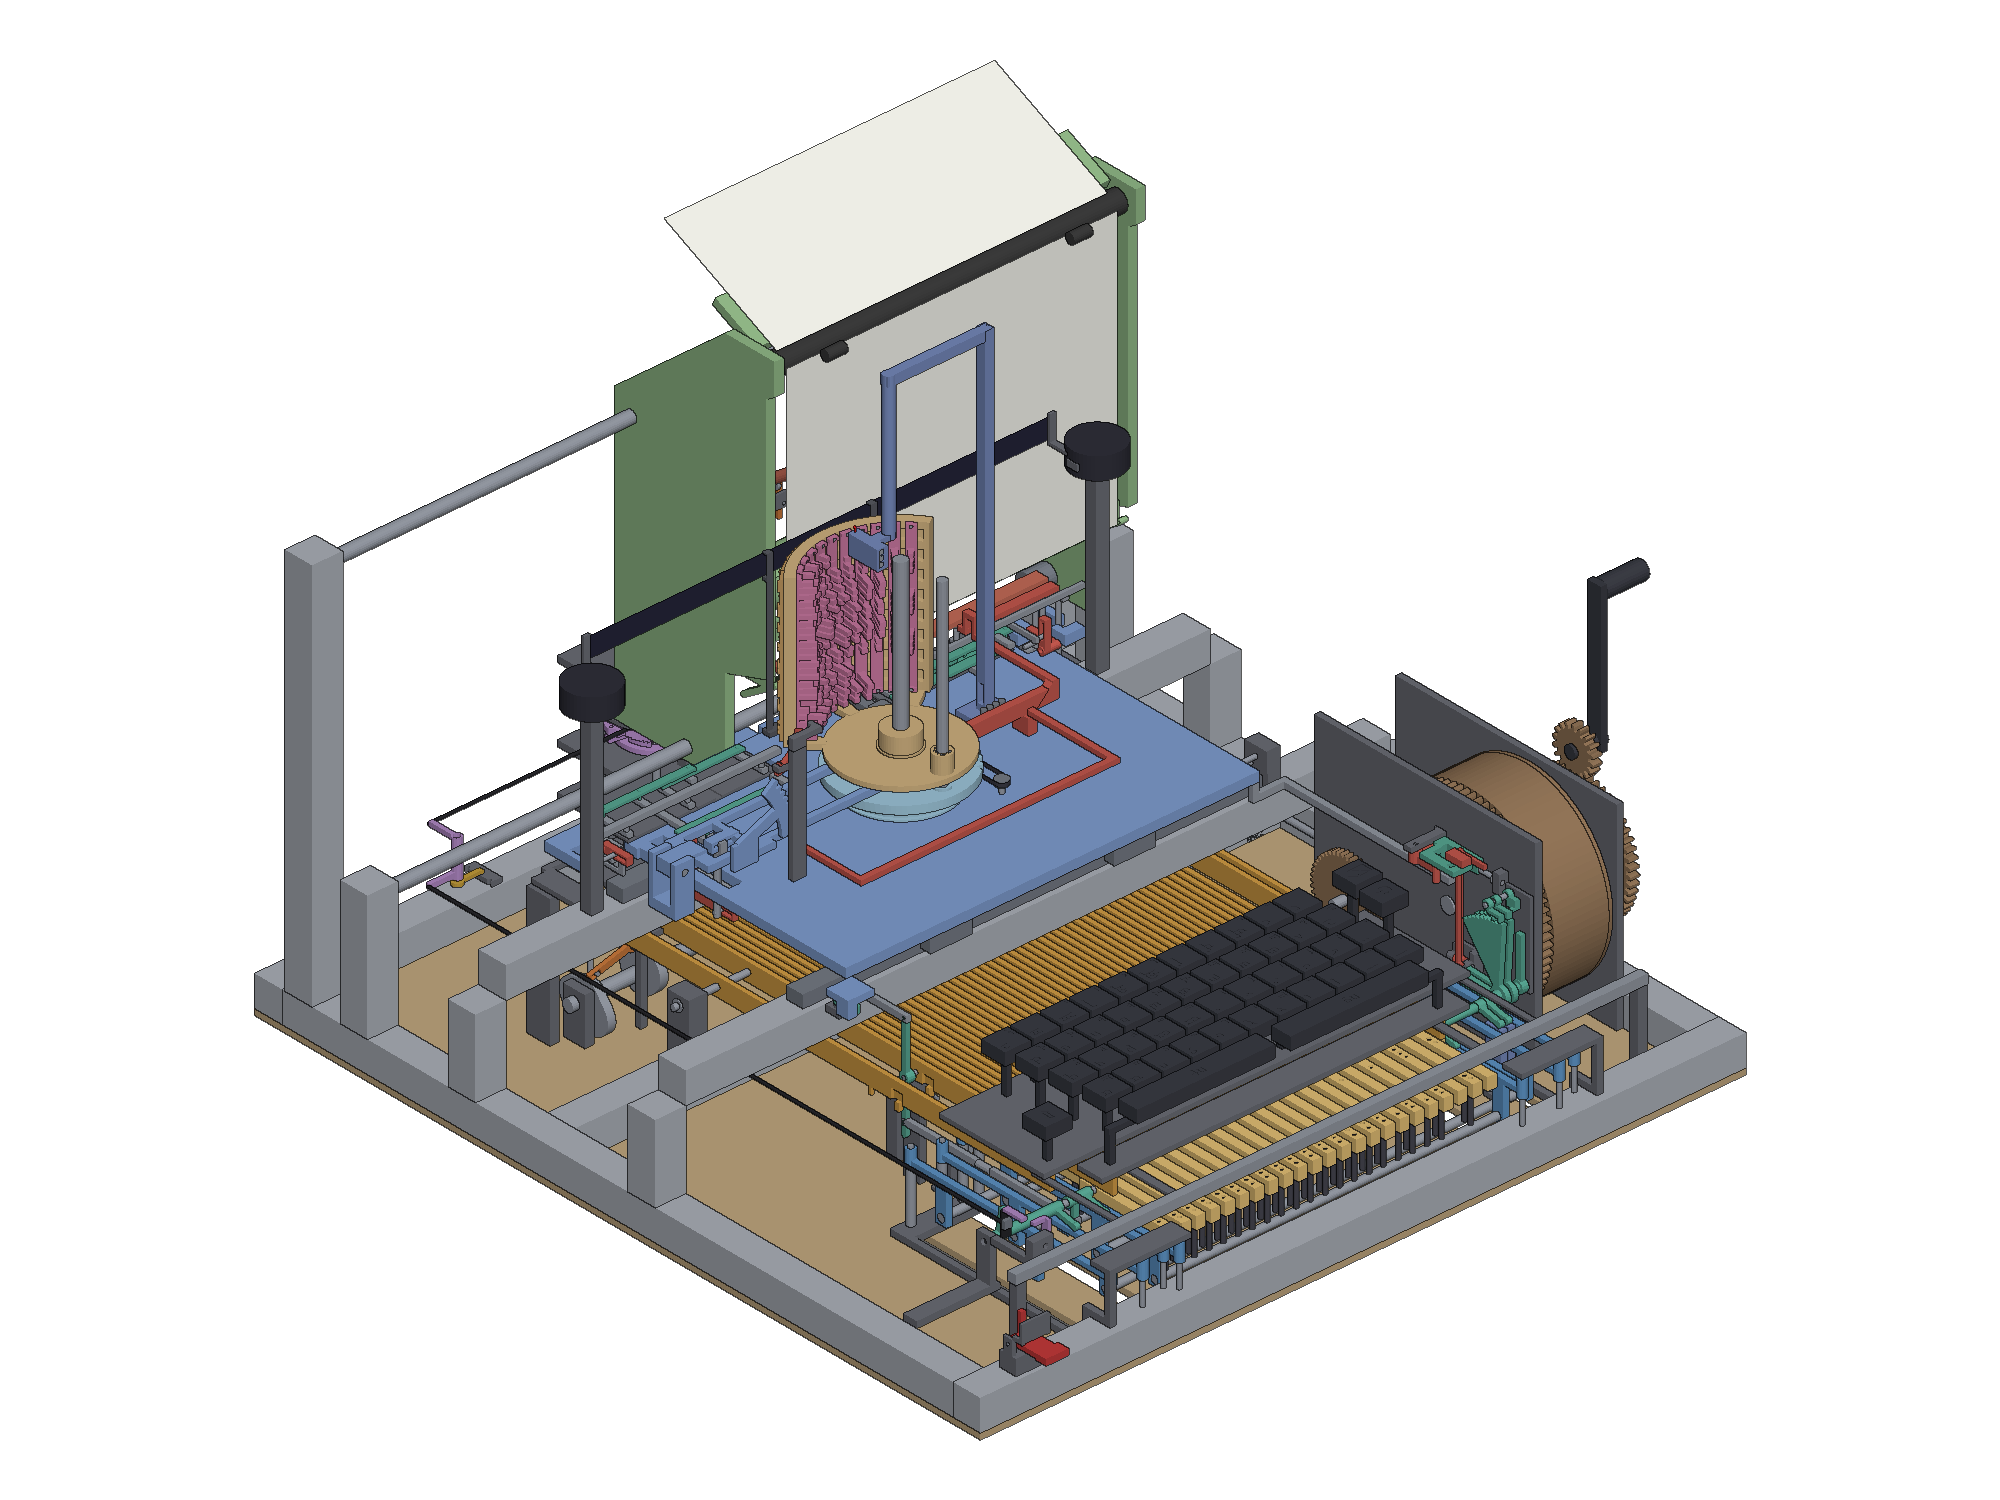
\includegraphics[width=\linewidth]{gen/model/renders/iso_front.png}
\caption{ТПМ-2 в модели, вид спереди слева. Рама из профиля 2020; впереди клавиатура, под ней рычаги, кодовые пластины и мерные рамки (голубые боковины); в середине печатающий узел на плите с направляющими (синий): челнок с литерными блоками, шкив и колесо фиксатора, коромысла; сзади каретка с кассетой бумаги, валиком и подставкой. Справа спереди — пружинный двигатель с ручкой завода, за ним сектора памяти.}
\label{fig:iso}
\end{figure}

\begin{figure}[H]
\centering
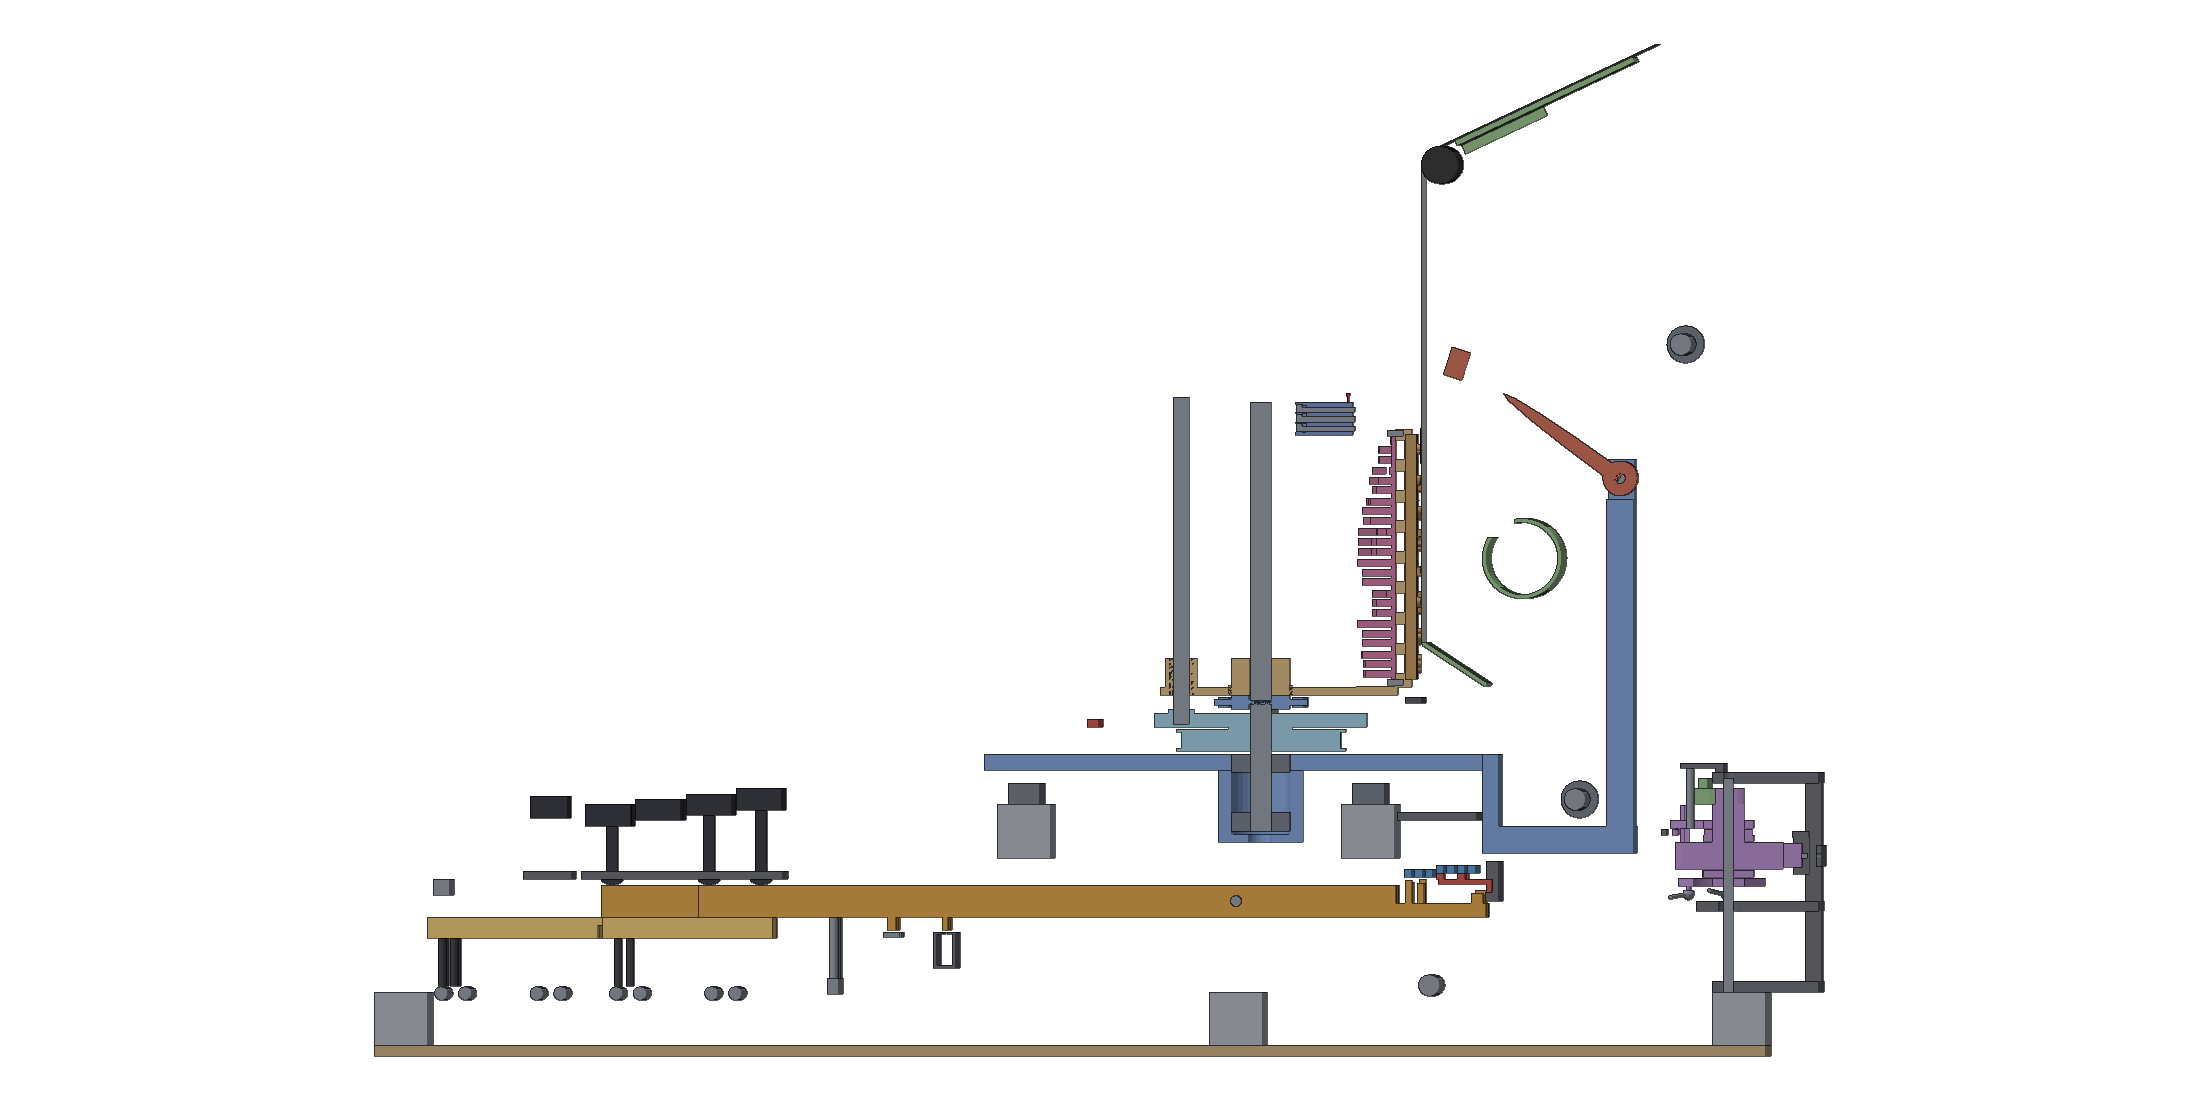
\includegraphics[width=\linewidth]{gen/model/renders/section_x0.png}
\caption{Разрез по оси удара. Слева направо: клавиши и гребёнка, рычаги (ось — кружок посередине), пластины и прутки рамок у пола, вал челнока в башне с двумя подшипниками, шкив и колесо фиксатора, плита узла на каретках MGN12, толкатель и планки выбора за осью рычагов, под ними цикловой вал, рычаг рамы под кассетой бумаги, молоток на стойке (взведён), лист от кассеты вверх к валику; справа — шестерня и колесо спуска.}
\label{fig:section}
\end{figure}

\subsection{Что изменила модель}

\begin{itemize}
  \item \textbf{Выбор позиции и ряда} — в 0.5 прямая линейка штифтов и лента барабана вместо полукруга под челноком; в 0.6 — коромысла с фиксаторами под цикловым валом (\S\ref{sec:select}).
  \item \textbf{Раскладка челнока}: 8 рядов по 11 позиций; позиция — столбец клавиши, ряд — ряд клавиши и регистр (рис.~\ref{fig:shuttle}).
  \item \textbf{Кодовая часть}: пластина под клавишей, ход 16~мм; два поля пластин; рамки из стальных прутков; выступы — установочные винты. В 0.10 код переехал на челнок: гребёнки на кольце, головка чтения внутри кольца, тросы к упору спуска и к ползункам B и C; поводок — за валом, диск кольца — под поясом (\S\ref{sec:read}).
  \item \textbf{Мёртвые знаки} сдвинуты на блоке на 8\,u, ход отвода 17\,u (9~мм).
  \item \textbf{Бумага} — кассета-труба под линией печати, как у Хаммонда; лист выходит вверх к валику, рычаг рамы проходит под кассетой к молотку. Валик поднят над верхним положением челнока.
  \item \textbf{Рама и узел}: профиль 2020, линейные направляющие для ползуна, плита узла из алюминиевого сплава. Печатать плиту не стоит: она несёт вал челнока и коромысла, и от её жёсткости зависит посадка знаков.
  \item \textbf{Видимость} (0.8): челнок в покое под строкой, лента опущена, ряды по частоте (\S\ref{sec:vis}).
  \item \textbf{Звенья} (0.8): коромысла на кулисах, рамки на вертикальных направляющих, сектора на соосных трубках у щеки двигателя, синусный рычаг к упору спуска, фиксатор ряда от тяги фиксатора позиции, запорная гребёнка (\S\ref{sec:links}).
  \item \textbf{Холостой цикл} (0.11): запоры чтения и удара построены деталями, сектор W снят, наборы блоков и гребёнок строятся для любого подходящего шрифта (\S\ref{sec:idle}, \S\ref{sec:fontsets}).
  \item \textbf{Двигатель} стоит справа спереди, рядом с ним сектора памяти; к цикловому валу он передаёт вращение валом вдоль правой стороны через две конические пары (рис.~\ref{fig:drive}).
\end{itemize}

\subsection{Проверка на пересечения}
\label{sec:checks}

Детали проверяются попарно: пересечение объёмом больше 0,05~мм$^3$ считается ошибкой, кроме оговорённых посадок (вал в подшипнике, винт в бобышке, штифт в направляющей). Кроме покоя модель прогоняется через состояния движения.

\begin{center}\small
\begin{tabularx}{\linewidth}{@{}Xrr@{}}
\toprule
Сценарий & состояний & пересечений \\
\midrule
\tabinput{gen/tab_model_checks.tex}
\bottomrule
\end{tabularx}
\end{center}

\noindent{\small Пересечений нет. С редакции 0.8 в каждом состоянии проверяются и пары движущихся деталей из разных групп движения (челнок с лентой, ползуны выбора с толкателями кулачков и т.\,п.); не построенными деталями остаются только включатели спуска, перечисленные в конце \S\ref{sec:back}, и в узле чтения — ролики тросов, трассы оболочек, запорный рычаг и связь задвижки (конец \S\ref{sec:read}).}

\subsection{Проверка касаний}
\label{sec:contacts}

Отсутствие пересечений ещё не значит, что механизм работает: если толкатель не достаёт до рычага, рычаг не пойдёт, и пересечения тоже не будет. Поэтому с редакции 0.9.1 модель проверяет ещё и касания (\code{tools/model/contacts.py}). Для каждой пары, где одна деталь ведёт другую, и для каждого состояния, где она должна вести, считается точное расстояние между поверхностями (библиотека FCL, по треугольникам) и объём перекрытия. Пара проходит, если зазор не больше 0,06~мм — столько оставляют грани круглых деталей, приближённых многоугольниками, — а перекрытие не больше 0,1~мм$^3$. Посадки (штифт, запрессованный в деталь, вал в отверстии) в список не входят: это соединения, а не касания.

Проверено \mncont\ пар, не прошло \mncontbad. В ходе проверки найдены и исправлены:
\begin{itemize}
  \item кулачки отставали от роликов на поворотах профиля: профиль теперь строится как кривая центра ролика, смещённая внутрь на радиус ролика; склоны кулачков фиксаторов (35°) и ленты (80°) удлинены, чтобы угол давления не превышал 45° (у кулачков поворота и подъёма — 38°);
  \item толкатель кулачка задевал качалку привода дерева: палец толкателя теперь в пазу качалки, а сама полка толкателя идёт низом, под размахом плеч, и поднимается к пальцу сбоку;
  \item тяга фиксаторов с наклоном 2:1 ход «растягивала» собачку: собачка стала жёстким ползуном с клином, наклон 1:1, ход тяги 3~мм, и клин собачки повторяет V-образный вырез колеса;
  \item пальцы в пазах угловых рычагов выходили за концы пазов при больших рядах: пазы удлинены до $\sqrt{h^2 + y^2}$;
  \item толкатель взвода молотка упирался в рычаг взвода с зазором 0,5~мм и терял касание на ходу: на толкателе теперь палец в радиальном пазу рычага, отношение ровно $r\tan\varphi$;
  \item у спуска собачка стояла в 0,5~мм от зуба, а переставной упор входил в тело зуба (\S\ref{sec:back}).
\end{itemize}

{\footnotesize\renewcommand\arraystretch{0.92}
\begin{longtable}{@{}>{\raggedright}p{92mm}rrrc@{}}
\toprule
Пара & состояний & зазор, мм & перекр., мм$^3$ & годна \\
\midrule
\endhead
\tabinput{gen/tab_contacts.tex}
\bottomrule
\end{longtable}}

\subsection{Удар: молоток, лист, лента, литера}
\label{sec:strike}

По схеме Хаммонда челнок — наковальня: молоток бьёт по листу сзади и вдавливает его вместе с лентой в литеру, вставшую против него. До редакции 0.9.2 модель проверяла из этой цепочки только касание бойка с листом, а оттиск на странице рисовался по условию «на таком-то угле цикла напечатан знак нажатой клавиши». Такое условие верно, только если челнок действительно подставляет под молоток нужную литеру и лента с листом до неё доходят, — а этого никто не проверял. Теперь проверяет модель (\code{tools/model/strike.py}): для каждой из 86 литер машинка ставится в момент удара (168° цикла), челнок повёрнут и поднят на код литеры так, как его выставляет выборка, и
\begin{itemize}
  \item цепочка боёк — лист — лента — литера должна быть замкнута: зазор в каждом звене не больше 0,06~мм, перекрытие не больше 0,1~мм$^3$ (лист и лента в окне молотка моделируются вдавленными им);
  \item часть лица литер, которой касается лента в окне молотка, проецируется на строку и сравнивается с рисунком самой литеры на её месте в клетке; не должно быть ни недостающего, ни лишнего (допуск 0,06~мм по контуру);
  \item ничто другое — ни соседние литеры, ни тело блока — не должно подходить к поверхности лица ближе 0,3~мм в окне молотка, расширенном на 0,8~мм во все стороны.
\end{itemize}
\begin{figure}[H]
\centering
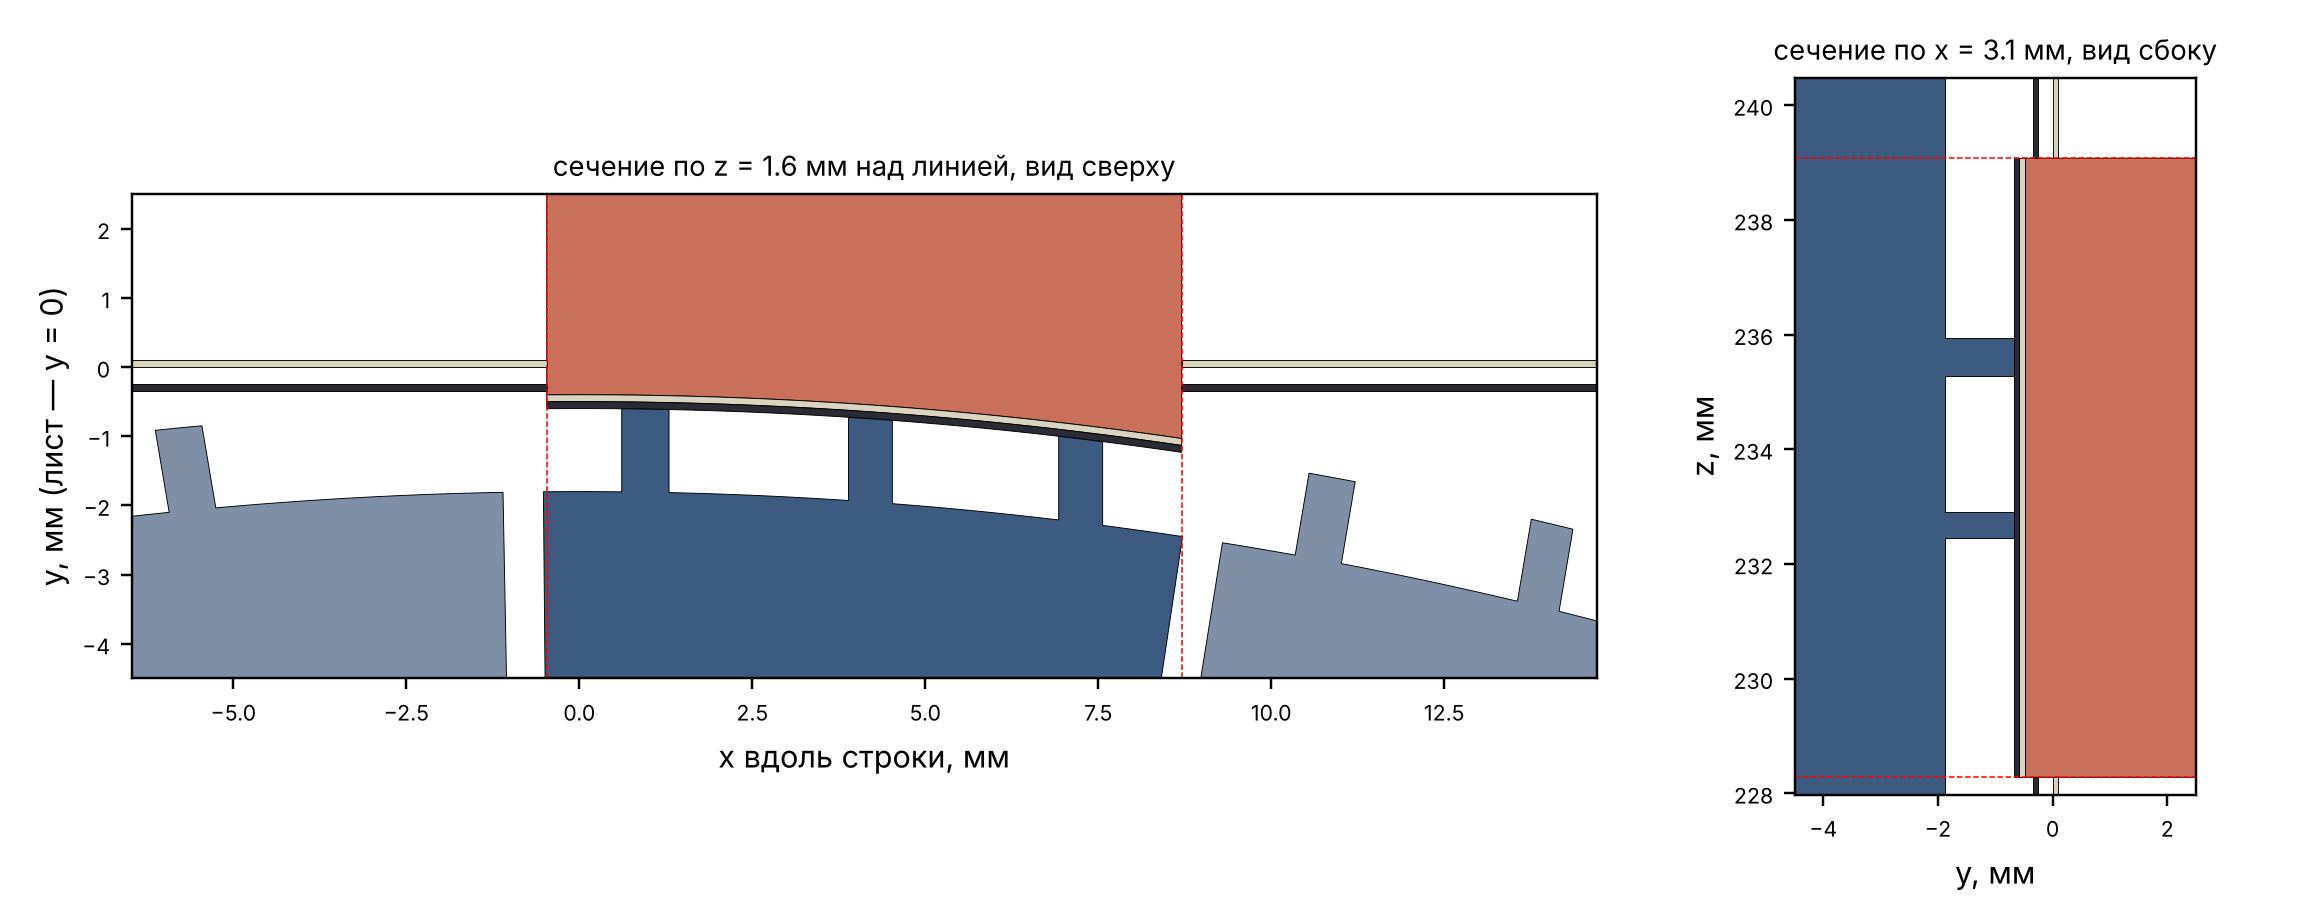
\includegraphics[width=\linewidth]{gen/model/renders/strike.png}
\caption{Удар в модели, литера ряда 6 позиции 4. Слева — сечение поперёк строки, вид сверху: вогнутый боёк (красный) прижал лист (светлый) и ленту (чёрная) к рельефу печатающей позиции (тёмно-синий); соседние блоки (серые) лежат вне окна молотка (красные штрихи) и ниже цилиндра лица. Справа — сечение вдоль высоты через ту же литеру; штрихами — окно молотка по высоте.}
\label{fig:strike}
\end{figure}

Проверено \mnstrike\ литер, не прошло \mnstrikebad. Что нашла проверка и что изменено:
\begin{itemize}
  \item на литерных блоках были отлиты только ряды 1--4: верхний регистр (ряды 5--8) отсутствовал, и при нажатом регистре челнок подставлял под молоток пустой блок;
  \item блоки стояли на челноке в обратном порядке: челнок, повёрнутый выборкой на позицию $m$, подставлял блок $10 - m$; знак поворота блоков на челноке исправлен;
  \item лицо блоков было плоским, и дальний край соседнего блока при повороте выходил вперёд лица печатающей позиции до 0,7~мм — прямо у края молотка; теперь лицо — цилиндр $R = 60$~мм вокруг оси челнока (рельеф 1,2~мм над цилиндром $R = 58{,}8$~мм), и соседние литеры уходят назад;
  \item лист висел в 1,5~мм перед литерами, а молоток доходил ровно до листа: ни лист, ни лента литеры не касались; зазор уменьшен до 0,6~мм, лента идёт посередине (0,25~мм до лица и до листа), лицо молотка вогнуто по цилиндру $R = 60{,}2$~мм вокруг оси челнока и в момент удара прижимает лист (0,1~мм) с лентой (0,1~мм) к литере по всему окну; резиновая накладка 1~мм на бойке выбирает неровности печати;
  \item окно молотка было шире оттиска (от $-1$ до $+17\,u$, по блоку) и подходило к соседним литерам на 0,2--0,7~мм; теперь оно подогнано к оттиску всех литер с запасом 0,1~мм (от $-0{,}9$ до $16{,}5\,u$ по строке и от $-2{,}9$ до $+6{,}2$~мм от линии шрифта по высоте; с 0.11 по высоте — от $-4{,}2$ до $+6{,}6$~мм ради других шрифтов, \S\ref{sec:fontsets}), и до оттиска соседних позиций остаётся около 1~мм, до соседних рядов — около 2~мм.
\end{itemize}
Запас 1~мм до соседней позиции — главное ограничение схемы: шаг позиций на лице челнока (10,05~мм) лишь на 1~мм больше оттиска самой широкой литеры. Хаммонд работал с такими же соседями; если на опытном оттиске соседняя литера всё же «прихватывает» краем, есть два средства: уменьшить зазор листа ещё (лист тогда меньше прогибается у края молотка) или увеличить шаг позиций, что удлиняет дугу челнока и ход поворота.

Цилиндрическое лицо печатается лицом вверх: при слое 0,1~мм на ширине литеры получается до семи ступенек по 0,1~мм. Ступеньки выбирает резиновая накладка бойка; для чистого оттиска лицо блоков можно пройти мелкой шкуркой по шаблону радиуса 60~мм.

{\footnotesize\renewcommand\arraystretch{0.92}
\begin{longtable}{@{}rrlrrrrrc@{}}
\toprule
ряд & поз. & литера & лента — литера, мм & площадь, мм$^2$ & нет, мм$^2$ & лишнее, мм$^2$ & чужое, мм$^3$ & годна \\
\midrule
\endhead
\tabinput{gen/tab_strike.tex}
\bottomrule
\end{longtable}}

\subsection{Номера, целостность и знаки на клавишах}
\label{sec:numbers}

\paragraph{Номера.} Каждая печатная деталь получает номер; он стоит в начале имени её файла STL (\code{042\_...stl}) и вдавлен в саму деталь на 0,6~мм — на верхнюю грань в положении печати, а если там нет места, на грань, которая лежит на столе (тогда зеркально, чтобы читался снизу). Под цифрами остаётся не меньше 1,2~мм материала, высота цифр — от 3 до 6~мм, шрифт PT Sans Bold. Для FDM вдавленные цифры надёжнее выпуклых: выпуклые на верхней грани требуют поддержки только если они нависают, но отрываются при печати и мешают посадке; вдавленные печатаются без поддержек и не меняют размеров детали. Из \mnprint\ деталей номер получили \mnnum\ (\mnnumtop\ сверху, \mnnumbot\ снизу); у \mnnonum\ мелких или узких деталей (планки 3~мм, штоки, пальцы) места для цифр нет — их номер есть только в имени файла и на сборочном листе.

\paragraph{Целостность.} Каждый файл STL — одно связное тело: сборка останавливается, если деталь распадается на части. В 0.9 так было у нескольких деталей — кодовых пластин, штоков клавиш, гребёнки стержней выбора, вилки подъёма, барабана пружины: их части касались друг друга только по грани или стояли порознь (так модель и рисует, но принтер напечатал бы два куска); теперь они связаны перемычками. Два файла из архива 0.9 при распаковке пропадали из-за двоеточия в имени конических пар «1:1» (недопустимо в Windows); имена файлов теперь состоят только из латиницы, цифр и знаков \code{\_+.-}.

\paragraph{Знаки на клавишах.} На колпачки вдавлены их знаки на 0,6~мм: нижний регистр крупно слева внизу, верхний мелко справа вверху, теми же контурами, что на литерных блоках, но утолщёнными до 0,8~мм на их размере, чтобы сопло 0,4~мм прошло каждую канавку. Одиночные техты увеличены до 1,8 раза. На служебных клавишах — {\symf ⇧}, {\symf ⌫}, {\symf ⟲} (DejaVu Sans Bold), на пробелах — «4u» и «6u».

\begin{figure}[H]
\centering
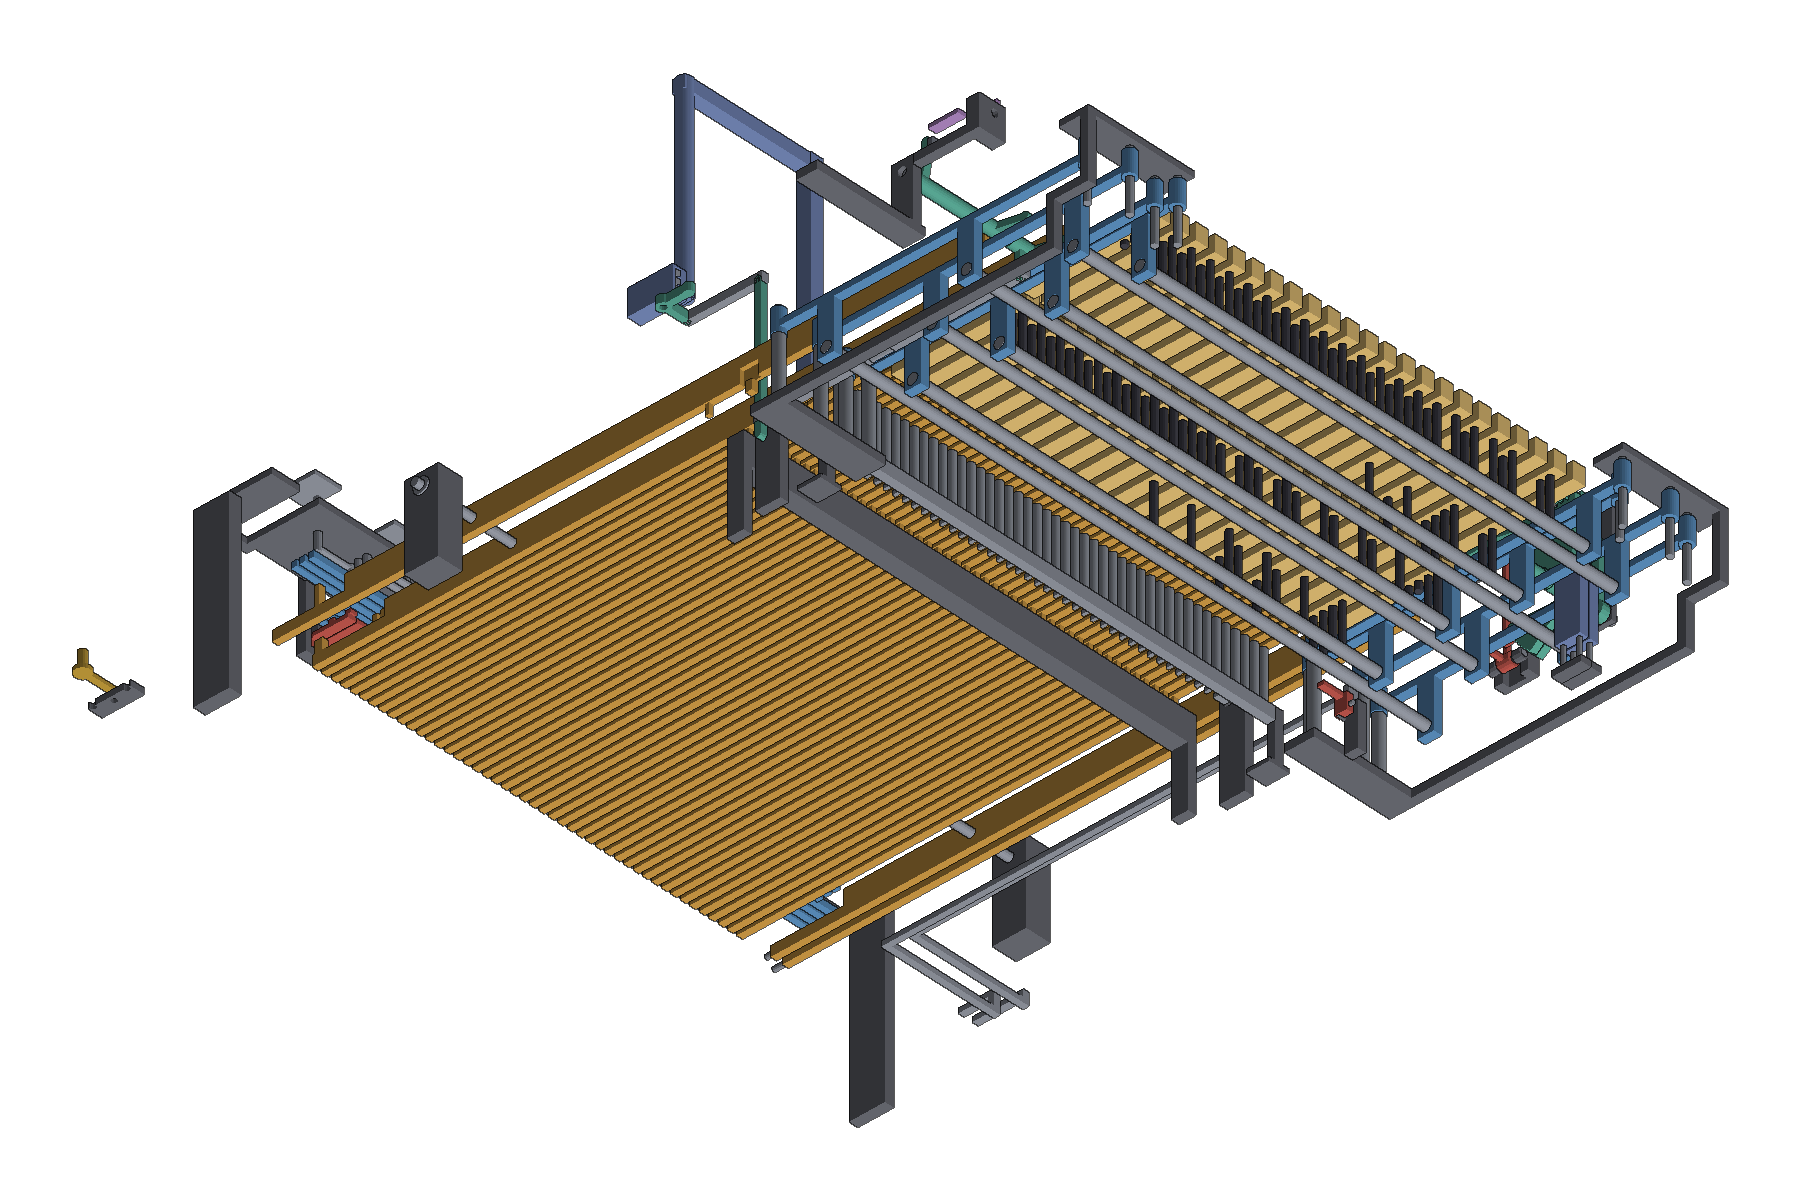
\includegraphics[width=0.78\linewidth]{gen/model/renders/code_under.png}
\caption{Кодовая часть снизу: рычаги, кодовые пластины двух полей с установочными винтами, стальные прутки мерных рамок с боковинами; справа — сектора памяти.}
\label{fig:codeunder}
\end{figure}

\subsection{Печать}

Все печатные детали уложены на стол 220$\times$220~мм: укладка выбирает положение с наименьшей высотой, литерные блоки и кодовые пластины печатаются в заданном положении (литеры лицом вверх). Рычаги длиннее стола и печатаются двумя частями с замком внахлёст на 20~мм; клавишная гребёнка — двумя частями.

\begin{center}\small
\begin{tabularx}{\linewidth}{@{}Xrrrr@{}}
\toprule
Группа & деталей & файлов STL & масса, г & габарит, мм \\
\midrule
\tabinput{gen/tab_model_print.tex}
\bottomrule
\end{tabularx}
\end{center}

\noindent{\small Масса — для сплошной печати PETG; при обычном заполнении крупных деталей она будет примерно вдвое меньше. Габарит — наибольший размер детали на столе.}

\subsection{Покупное и нарезаемое}

{\footnotesize\renewcommand\arraystretch{0.92}
\begin{longtable}{@{}>{\raggedright}p{70mm}r>{\raggedright\arraybackslash}p{80mm}@{}}
\toprule
Изделие & кол-во & примечание \\
\midrule
\endhead
\tabinput{gen/tab_model_buy.tex}
\bottomrule
\end{longtable}}
\label{tab:buy}

\noindent{\small Пружины, крепёж рамы и стыков, красящая лента в перечень не входят. Габарит рамы — 500$\times$525~мм; без корпуса, с выступающими ручкой завода (справа, +49~мм), клавишей освобождения каретки (спереди, +17~мм) и кронштейном спуска (сзади, +21~мм) — 549$\times$563~мм. С корпусом (\S\ref{sec:case}) — \mextw$\times$\mextd~мм: корпус \mcasew$\times$\mcased~мм, справа за ним остаётся ручка завода. Высота с подставкой бумаги — \mheight~мм, корпус с навершиями пилястр — \mcaseh~мм. Каретка ходит внутри рамы и за её габарит не выходит.}

\paragraph{Бумага.} Машинка рассчитана на лист шириной до 220~мм: такова прорезь кассеты-трубы и направляющая; в модели лежит лист 216~мм (Letter, 8,5\,дюйма), лист A4 (210~мм) входит так же. Строка — 170~мм (20~em, 321\,u): на A4 остаётся по 20~мм полей с каждой стороны, если упоры полей не переставлены. По частотам из двух книг (\S\ref{sec:freq}) средняя продвигающая литера Alcarin — 9,9\,u, и полная строка текста вмещает около 57 нажатий: 22 продвигающие литеры, 18 техтар (они не двигают каретку) и 17 пробелов; у узких шрифтов (Miriel, Hanno) — 67--70 нажатий. Длина листа не ограничена: лист сворачивается в кассете, строки подаются валиком, по вертикали он и выставляется валиком.

%=====================================================================
\section{Пружинный двигатель и цикл}
\label{sec:motor}
\label{sec:dyn}

\subsection{Почему пружина}

В редакции 0.5 челнок 4$\times$22 радиусом 107~мм имел момент инерции около \mIold~кг$\cdot$мм$^2$. Чтобы повернуть его к литере за долю хода клавиши, нужно больше джоуля на знак, а палец отдаёт на весь ход 0,01--0,02~Дж. Поэтому энергию на челнок даёт заводная пружина, а клавиша только набирает код и спускает цикл. Чтобы завода хватало надолго, челнок перестроен под минимальную энергию (\S\ref{sec:size}): 8$\times$11, радиус 60~мм, блоки толщиной 4~мм, кольцо с окнами.

\begin{center}\small
\begin{tabular}{@{}lr@{}}
\toprule
Поворотная часть (ред. 0.6) & $I$, кг$\cdot$мм$^2$ \\
\midrule
\tabinput{gen/tab_motor_I.tex}
\bottomrule
\end{tabular}
\end{center}

\noindent{\small По модели; кольцо и шкив — заполнение 50\,\%, блоки — сплошные. Подъёмная масса (кольцо, блоки, втулка, вилка) — \mmlift~г.}

\subsection{Цикл}

Цикловой вал делает оборот на каждый удар. Пружина держит на нём постоянный момент, защёлка держит его в покое; последняя точка хода клавиши спускает защёлку, после оборота упор на валу снова ложится на неё. Кулачки по циклоидному закону (без ударов) ведут приводные планки коромысел туда и обратно, вводят фиксаторы, выпускают и втягивают щупы чтения, взводят и спускают молоток; в конце оборота дают ход подаче каретки и возврату ползуна.

\begin{figure}[H]
\centering
\begin{tikzpicture}[x=5mm,y=1mm]
\draw[ink!50,->] (0,0) -- (18.6,0);
\foreach \a in {0,45,...,360} {\draw[ink!50] (\a/20,0) -- (\a/20,-1.5) node[lbl,below]{\a};}
\node[lbl,anchor=north] at (9,-5) {угол циклового вала, градусы};
\node[lbl,anchor=east] at (-0.2,40) {поворот и подъём челнока: туда};
\fill[accent!35] (0.5,38.4) rectangle (6.0,41.6);
\node[lbl,anchor=east] at (-0.2,33) {обратно в исходное};
\fill[accent!20] (10.0,31.4) rectangle (15.5,34.6);
\node[lbl,anchor=east] at (-0.2,26) {фиксаторы, подъём ленты};
\fill[sledB!40] (5.5,24.4) rectangle (9.75,27.6);
\node[lbl,anchor=east] at (-0.2,19) {взвод молотка};
\fill[axisred!25] (0.5,17.4) rectangle (7.5,20.6);
\node[lbl,anchor=east] at (-0.2,19) {};
\fill[axisred] (7.95,17.4) rectangle (8.05,20.6);
\node[lbl,anchor=east] at (-0.2,12) {подача каретки, возврат ползуна, сброс};
\fill[axisblue!45] (15.5,10.4) rectangle (17.5,13.6);
\node[lbl,anchor=east] at (-0.2,5) {защёлки разрядов};
\fill[ink!30] (0.0,3.4) rectangle (0.4,6.6);
\node[lbl,anchor=east] at (-0.2,-2) {клавиатура заперта};
\fill[ink!12] (0.25,-3.6) rectangle (17.25,-0.3999999999999999);
\node[lbl,anchor=east] at (-0.2,54) {щупы читают код с челнока};
\fill[sledA!25] (5.9,52.4) rectangle (9.85,55.6);
\node[lbl,anchor=east] at (-0.2,54) {};
\fill[sledA!60] (7.0,52.4) rectangle (7.5,55.6);
\node[lbl,anchor=east] at (-0.2,47) {задвижка держит ширину};
\fill[sledA!15] (7.0,45.4) rectangle (17.25,48.6);

\end{tikzpicture}
\caption{Цикл. Тёмная риска в строке молотка — удар (160°). Время оборота зависит от знака: в среднем \mtavg~с, для дальней литеры в крайнем ряду — \mtworst~с, без перемещения челнока — \mtlight~с.}
\label{fig:cycle}
\end{figure}

\paragraph{Регулятор.} Без нагрузки пружина раскрутила бы вал слишком быстро, поэтому через пару 32/8 на валу сидит воздушный регулятор — четыре лопасти, чьё сопротивление растёт с квадратом скорости; он ограничивает оборот без нагрузки 0,18~с. Маховика нет: вал останавливается после каждого удара, и маховик приходилось бы разгонять заново.

\paragraph{Энергия на знак.} Пружина держит на валу постоянный момент, и за оборот отдаёт $2\pi\tau$ независимо от знака: часть уходит на потери в кулачках при разгоне и торможении челнока (КПД передачи принят \meta\,\%), на взвод молотка (\mEhammer~мДж), с ред. 0.10 — на щупы чтения (в среднем \rdEavg~мДж, \S\ref{sec:read}) и трение, остальное гасит регулятор. Время оборота считалось интегрированием движения вала с приведённой инерцией челнока для каждой из 86 литер и для пробела (с ред. 0.11: холостой цикл к позиции 0 первого ряда, \S\ref{sec:idle}); средние взяты с весами частот нажатий из книг, пробелы — \fqSP\,\% (\S\ref{sec:freq}), а момент подобран так, чтобы и средний, и худший знак укладывались в разумное время.

\begin{center}\small
\begin{tabular}{@{}rrrrrr@{}}
\toprule
$\tau$, мН$\cdot$м & мДж на знак & без хода, с & средний, с & худший, с & знаков на завод \\
\midrule
\tabinput{gen/tab_motor_sim.tex}
\bottomrule
\end{tabular}
\end{center}

\noindent{\small Выделен выбранный момент: средний знак — \mtavg~с (\mcpsavg\ знака в секунду, около 150 в минуту), худший — \mtworst~с.}

\subsection{Пружина и передача}

\begin{center}\small
\begin{tabularx}{\linewidth}{@{}lX@{}}
\toprule
\tabinput{gen/tab_motor_spring.tex}
\bottomrule
\end{tabularx}
\end{center}

\noindent{\small Энергия пружины — по пределу $\sigma^2/6E$ для изгиба полосы при $\sigma = 1500$~МПа; в работу берётся половина (неравномерный изгиб, трение витков). КПД передачи — 0,93 на ступень.}

\paragraph{Итог.} Одного завода хватает примерно на \mcharswind\ нажатий, считая пробелы (из них около 70\,\% — знаки, остальное пробелы) — две трети машинописной страницы; завод — \mcrankturns\ оборотов ручки через пару 1:3, усилие на ручке до \mcrankforce~Н. Пружина в барабане Ø120~мм справа спереди, под правой рукой, как у граммофона. Барабан закрыт: в заведённой пружине около 150~Дж, и при обрыве незакрытая пружина опасна; храповик завода имеет отпускную собачку для безопасного спуска.

\begin{figure}[H]
\centering
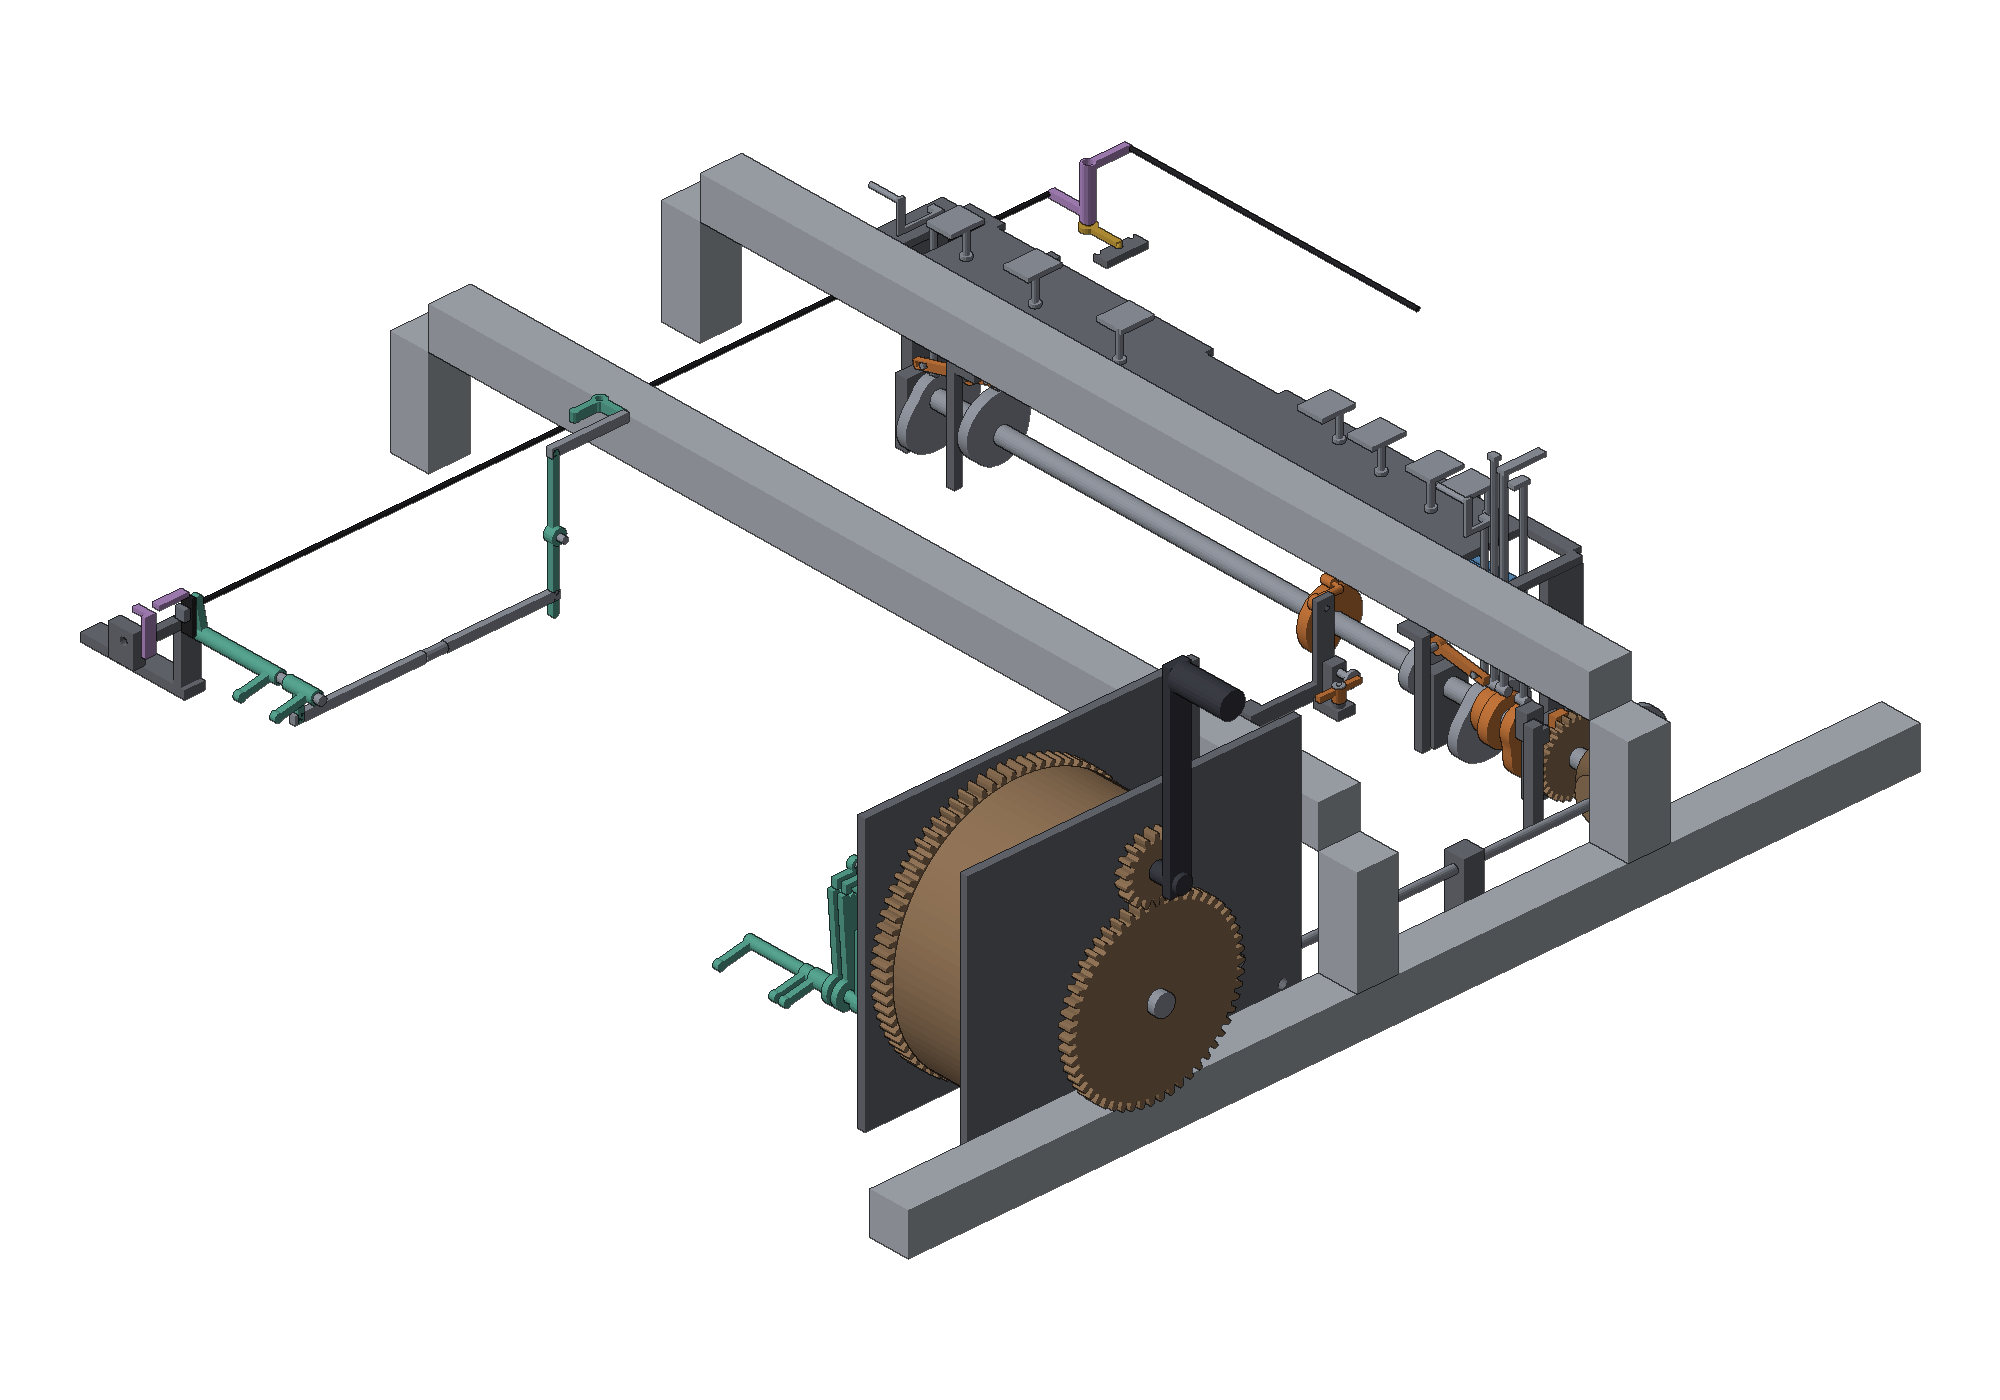
\includegraphics[width=0.85\linewidth]{gen/model/renders/drive.png}
\caption{Двигатель в модели: барабан с пружиной и ручкой завода (через пару 1:3), первая ступень $m = 1{,}5$ между щёк, вторая ступень, коническая пара на промежуточный вал вдоль правой стороны, вторая коническая пара на цикловой вал; на цикловом валу — регулятор, упор цикла и пять кулачков с толкателями.}
\label{fig:drive}
\end{figure}

\paragraph{Чего не хватает.} КПД кулачков, трение и энергия удара молотка — допущения; от них прямо зависит число знаков на завод. Их даст стенд этапа Э5. Если запаса окажется мало, есть три рычага: замедлить цикл (при среднем обороте 0,5~с завода хватает примерно на 1400 знаков), поставить второй барабан параллельно или уменьшить подъём, перейдя на 6 рядов по 15.

\subsection{Прочность}

\begin{itemize}
  \item \textbf{Зубчатые колёса двигателя.} На колесе барабана при наибольшем моменте пружины 5,1~Н$\cdot$м усилие на зубе около 85~Н; при модуле 1,5 и ширине 8~мм напряжение изгиба в PETG около 25~МПа — запас двукратный. Вторая и третья ступени нагружены в 7 и 27 раз меньше.
  \item \textbf{Мерные рамки.} Стальной пруток 5~мм на пролёте 276~мм под нагрузкой 0,3~Н прогибается на \mdbar~мм — на порядок меньше допуска кода. Печатная планка того же сечения прогнулась бы на миллиметры; поэтому прутки стальные.
  \item \textbf{Рычаги.} Консоль 60~мм сечения 3$\times$12~мм из PETG под 1~Н — \mdlev~мм; на код не влияет, так как пластина висит под клавишей.
  \item \textbf{Литеры.} При пиковом усилии молотка 120~Н на рельеф около 20~мм$^2$ напряжение около \msigtype~МПа при пределе текучести PETG около 50~МПа; запас есть, но износ рельефа под ударом через ленту можно узнать только испытанием (этап Э4).
  \item \textbf{Фиксатор челнока} работает на остановленном челноке и доворачивает его не больше чем на пол-позиции; ударной нагрузки на нём нет — в этом главное преимущество кулачкового привода перед остановом на штифте.
\end{itemize}

%=====================================================================
\section{Корпус}\label{sec:case}

С редакции 0.12 у машинки есть оболочка в нолдорском духе. Она надета на раму и не трогает ни одной движущейся детали: корпус — часть модели и проходит все её проверки вместе с механизмом (\S\ref{sec:checks}), включая покой и все сценарии движения; на странице модели его можно показать, сделать стеклянным или скрыть.

\begin{figure}[H]
\centering
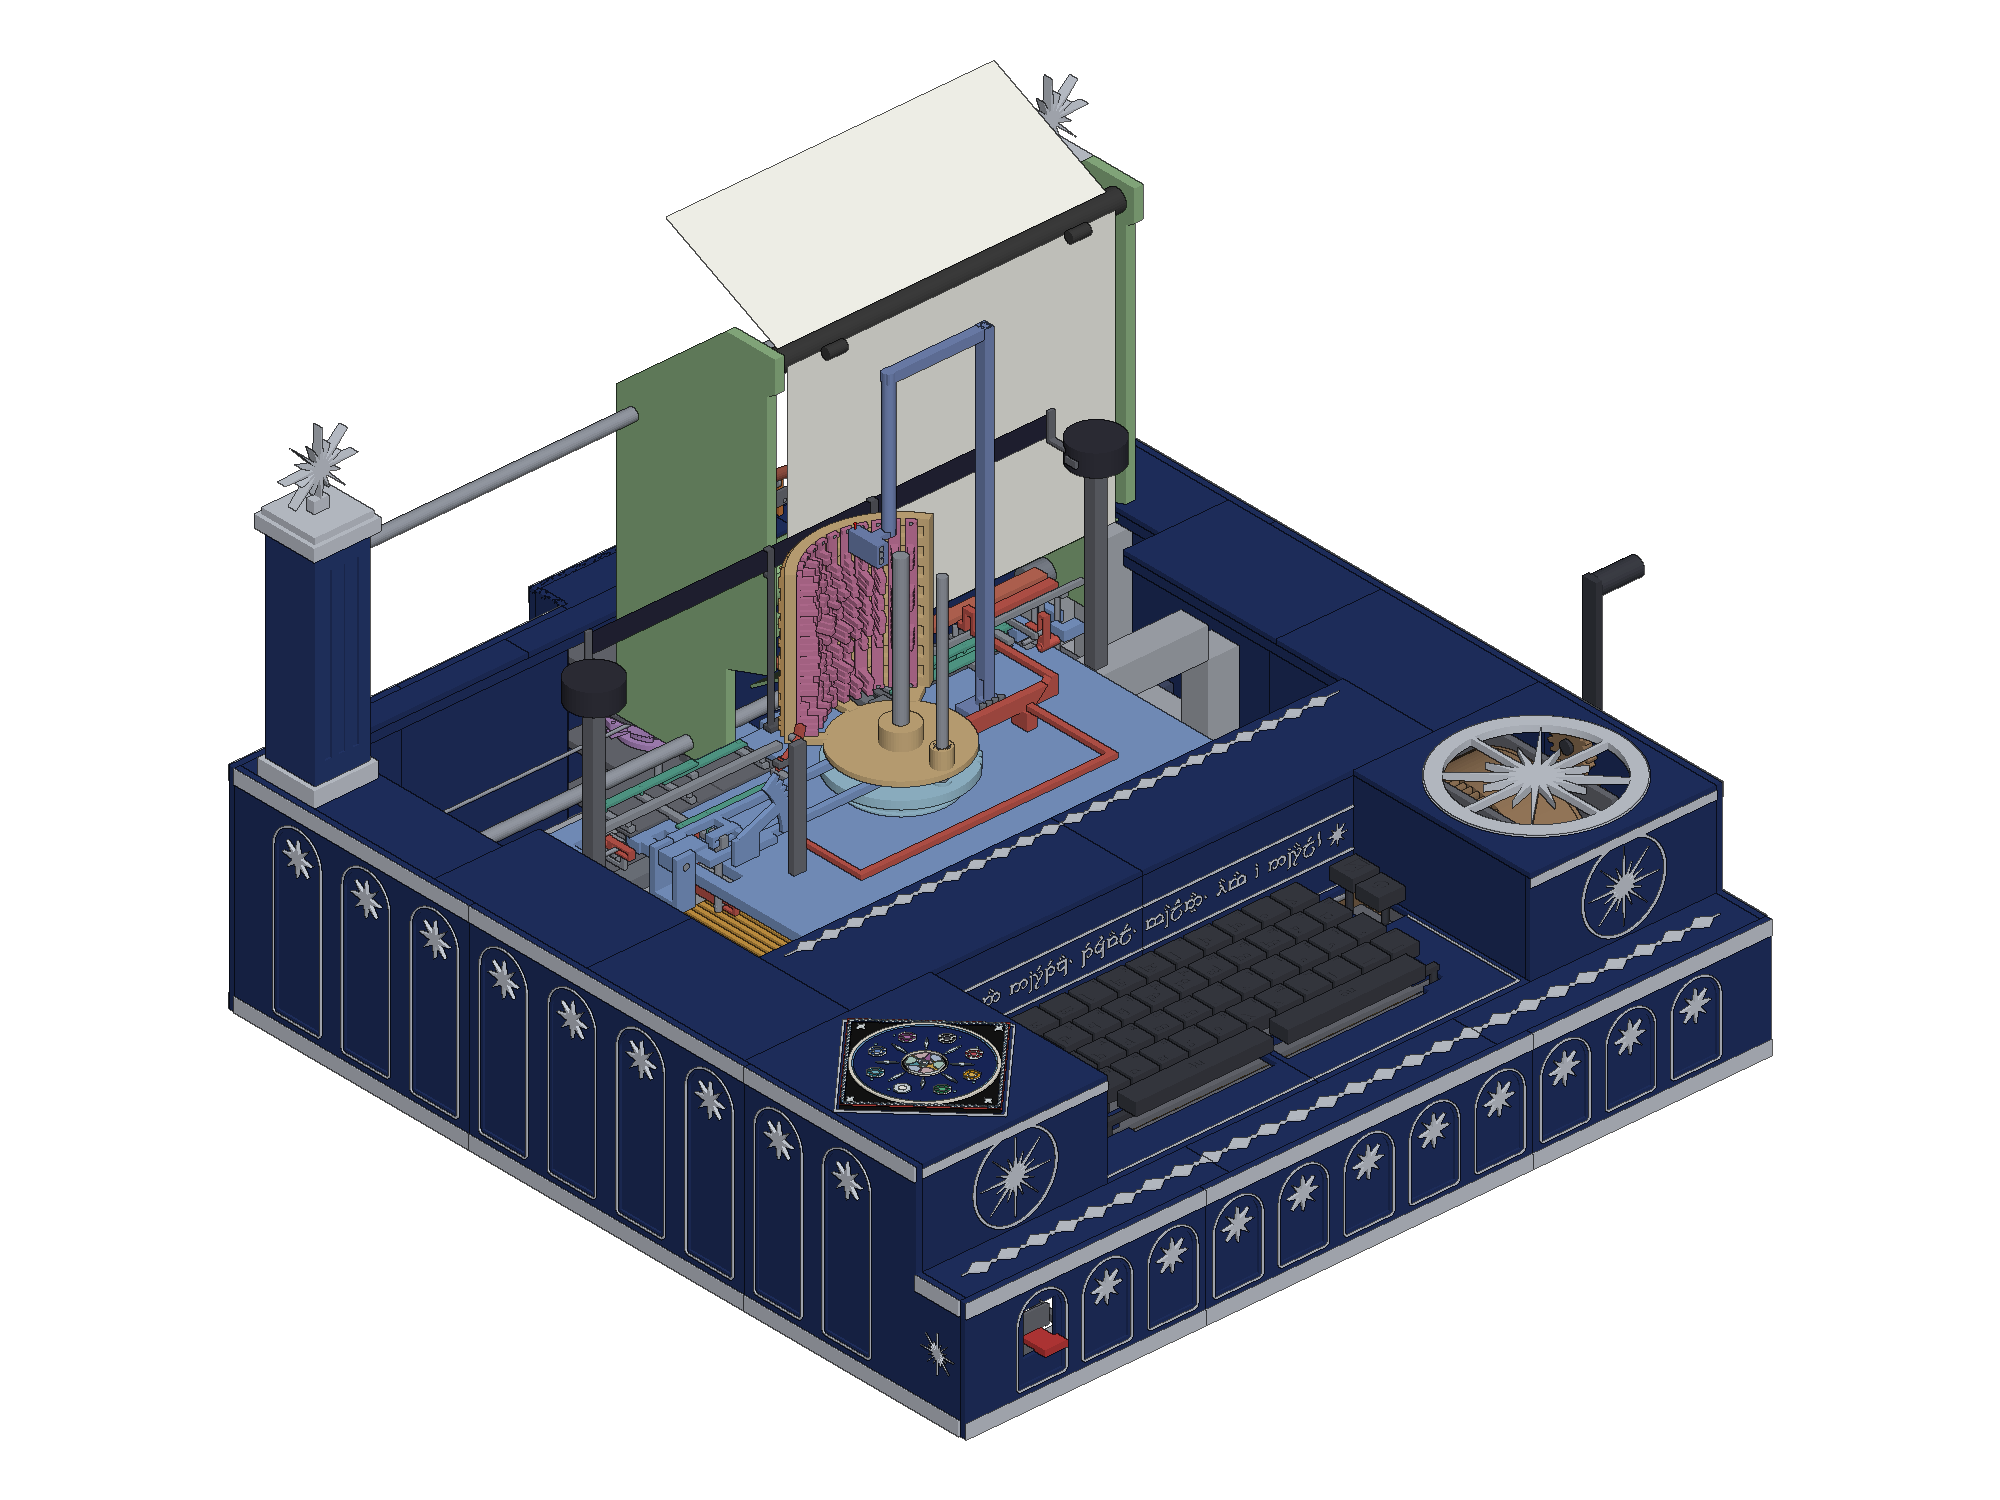
\includegraphics[width=\linewidth]{gen/model/renders/case_iso_front.png}
\caption{ТПМ-2 в корпусе, вид спереди слева. Впереди — колодец клавиш между двумя башнями: на левой щит с гербом, на правой решётка-звезда над барабаном пружины; за клавишами — лицо с надписью; двор над печатающим узлом и проём каретки открыты; над стойками каретки — пилястры с навершиями-звёздами.}
\label{fig:case}
\end{figure}

\paragraph{Из чего состоит.} Низ — четыре стенки толщиной 4~мм вокруг рамы: передняя высотой 78~мм, боковые и задняя — 140~мм; стенки стоят на упорах, привёрнутых в пазы профиля (упоры в модели есть, винты М5 с Т-гайками — нет), и обходят то, что выступает за раму: правая стенка, как и левая, отнесена на 11~мм от рамы, за ней шестерни завода, а ручка завода остаётся снаружи, её вал проходит сквозь нишу; клавиша освобождения каретки выходит сквозь нишу передней стенки; спуск, выступающий за раму назад, накрыт эркером. Клавиши стоят в колодце: дека колодца на высоте 78~мм, на 4--18~мм ниже клавиш, с отверстием по каждой клавише и штоку пробела; по бокам колодца — две башни высотой 140~мм, впереди — полоса под ладони. Верхняя дека (140~мм) обходит двор над печатающим узлом ($\pm$192~мм, от 170~мм перед осью до оси) и проём каретки ($\pm$216~мм): челнок, лента и лист видны пишущему, как и без корпуса: расчёт видимости (\S\ref{sec:vis}) с корпусом даёт те же цифры, ни одна его деталь не заслоняет строку ни с одной из трёх посадок. Свободные края деки держат рёбра снизу. Пилястры над стойками каретки пустотелые и надеты на стойки, верхний пруток каретки входит в пилястру через отверстие.

\paragraph{Орнамент.} Весь геометрический, в духе нолдорских знаков: звёзды восьми и шестнадцати лучей (как звезда дома Феанора — восемь длинных лучей и восемь коротких), ниши с полуциркульным верхом, цепь ромбов. По стенкам идёт аркада ниш со звездой в каждой, над цоколем и под карнизом — серебряные пояса; на лицах башен — большие звёзды в кольцах, на эркере — такая же; вдоль края двора и по полосе под ладони — цепь ромбов. Пилястры с каннелюрами, база, капитель и навершие — серебро.

\paragraph{Надпись.} На лице за клавишами, перед глазами пишущего, — надпись на квенья:
\begin{center}\emph{si na níretequa: tecuvalye, málonya, aima i níralye!}\\
«Это силовая кисть: пиши, друг мой, что угодно, что пожелаешь!»\end{center}
Здесь игра слов: \emph{níre} — сила, давление, поэтому \emph{níretequa} («силовая кисть») — печатная машина; \emph{níra} — «хотеть»; \emph{tequa} однокоренное с \emph{tec-} «писать». Надпись набрана так, как её напечатала бы сама машинка: страница модели переводит текст в знаки раскладки (классический режим квенья), положение каждого знака — по ширинам и отводам машинки, рисунок — Alcarin; затем всё увеличено в \minsk~раза, до \minsw~мм. Те же 52 знака можно напечатать на странице модели.

\begin{figure}[H]
\centering

\includegraphics[width=\linewidth]{gen/model/renders/case_fascia.png}
\caption{Лицо за клавишами с надписью; по краям — восьмилучевые звёзды.}
\label{fig:casefascia}
\end{figure}

\paragraph{Герб.} На левой башне — щит с гербом автора, Mírë Nolmeo (двенадцатая редакция): ромб 112~мм по диагонали. Рисунок перенесён из SVG без перерисовки: \code{tools/device.py} растрирует его, относит каждую точку к ближайшему цвету самого рисунка и обводит области (\mdevcol~цвета, \code{data/device/device\_regions.json}). Поле щита — основание толщиной 2,4~мм, каждый цвет — рельеф над ним высотой 0,3--1,2~мм по светлоте: тёмное ниже, светлое выше, как на камее. Самые тонкие черты — пряди каймы — около 0,6~мм. Щит печатается многоцветной печатью: в \code{stl/device/} по файлу на цвет с общим началом координат, их загружают как части одного предмета.

\begin{figure}[H]
\centering

\includegraphics[width=0.62\linewidth]{gen/model/renders/case_device.png}
\caption{Щит с гербом на левой башне (вид сверху).}
\label{fig:casedevice}
\end{figure}

\paragraph{Печать и сборка.} Корпус — \mcasepieces~печатных деталей (\mcasepmass~кг PETG при сплошной печати; масса механизма — \mmechmass~кг), все укладываются на стол 220$\times$220~мм: стенки и деки разрезаны по промежуткам между нишами и клавишами; швы скрепляются накладками на винтах (в модели их нет). Серебро печатается вместе с панелью: панель лежит лицом вверх, весь орнамент выше лица, и на этой высоте меняется пруток; пилястры, базы, капители, навершия и решётка — целиком серебристым PETG. Номера деталей у корпуса оттиснуты только на тыльной стороне. Деки снимаются: под ними всё, что регулируется при сборке (\S\ref{sec:adjust}), — сектора памяти и упоры под правой башней, спуск под задней полосой и эркером.

\begin{figure}[H]
\centering
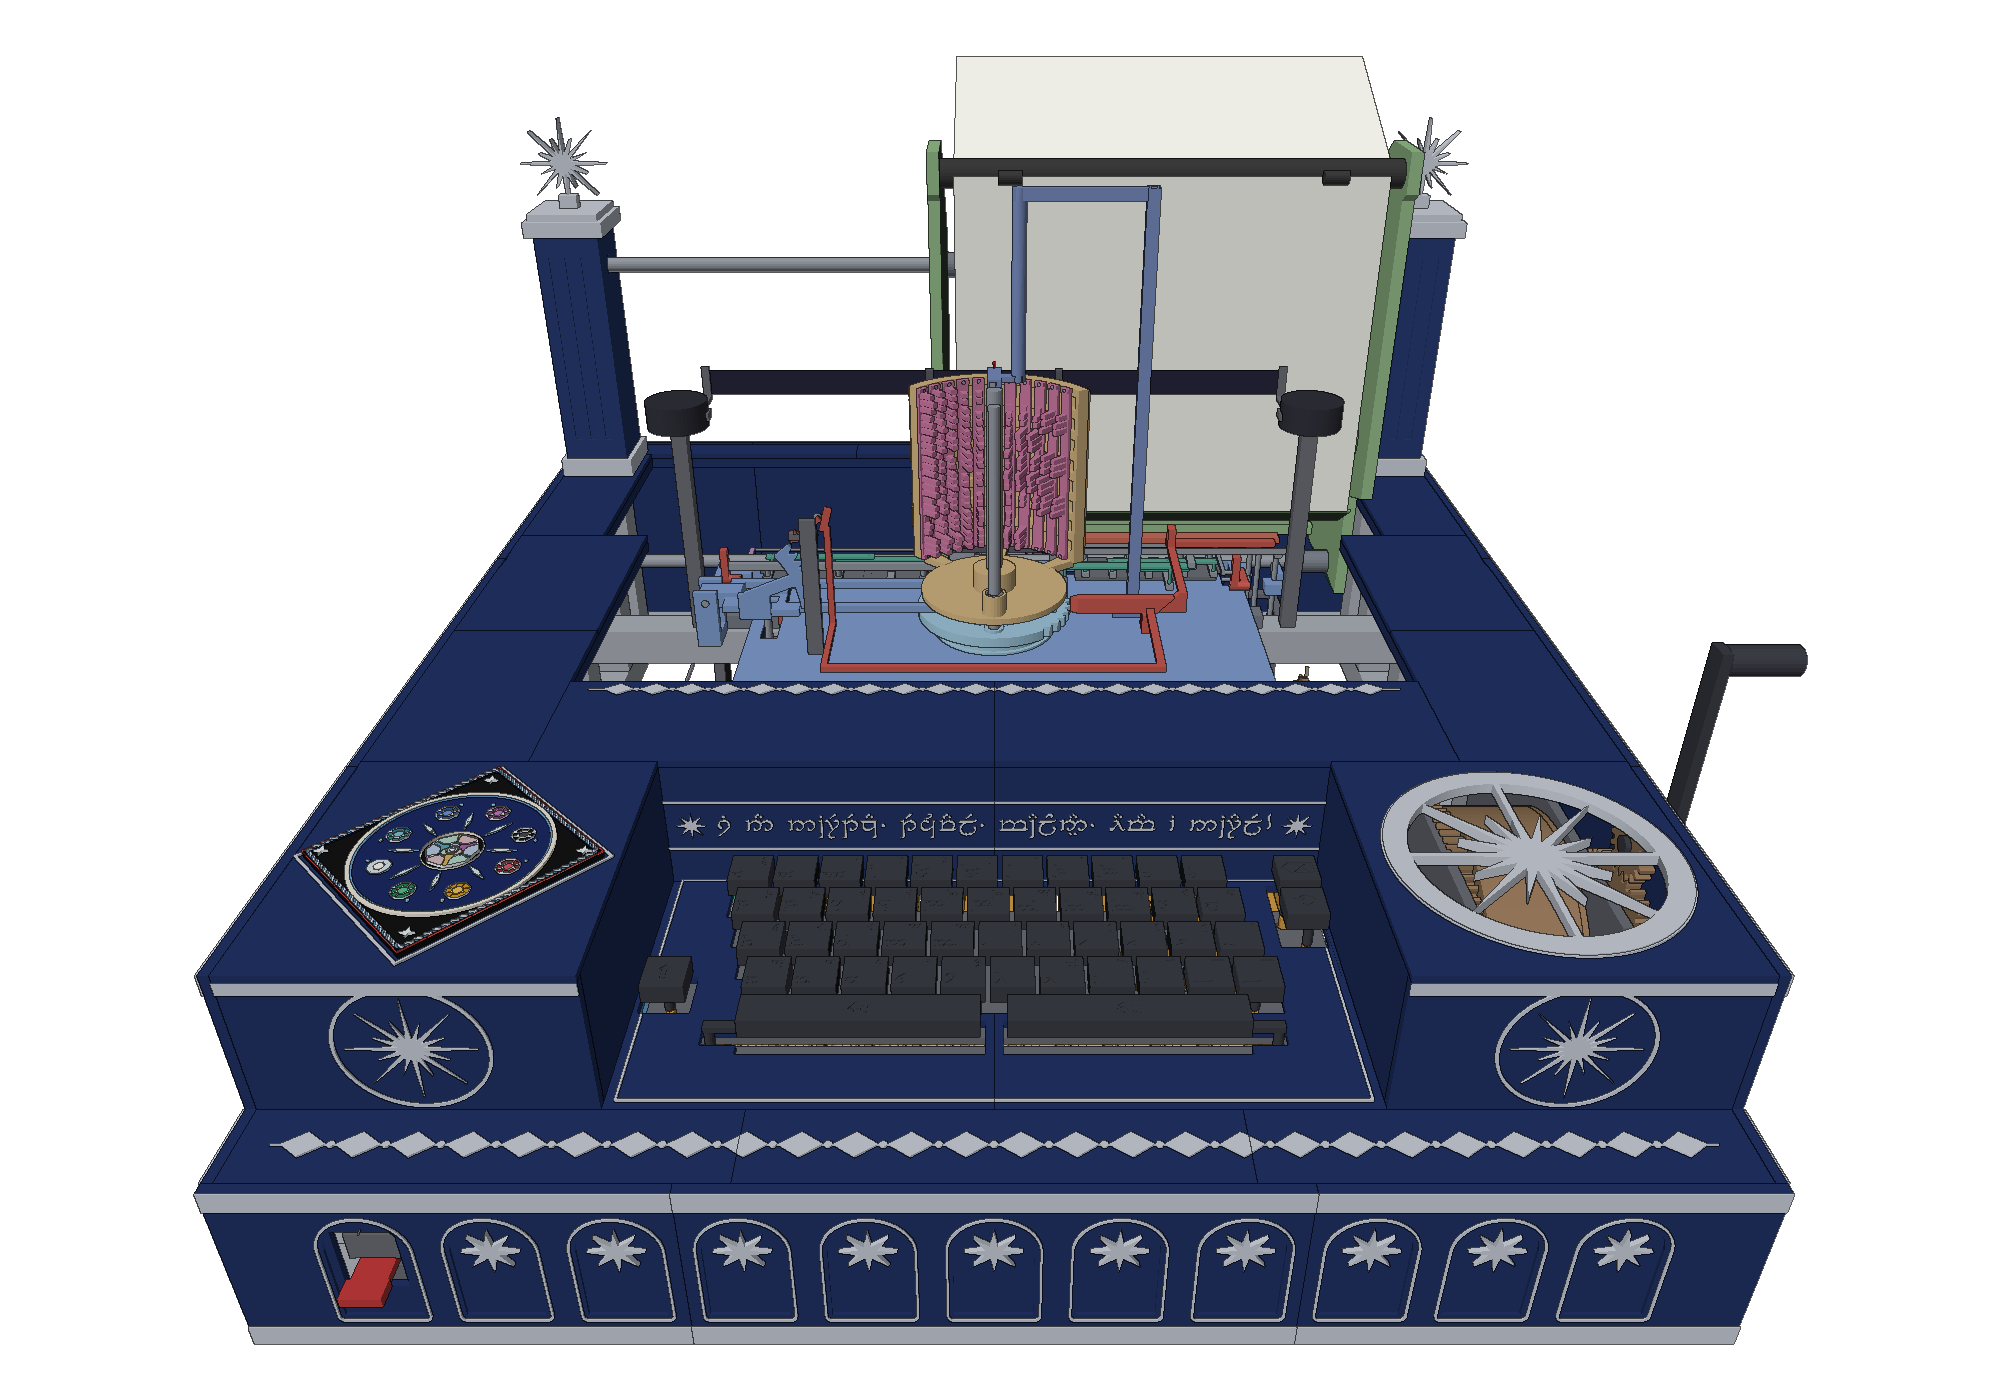
\includegraphics[width=\linewidth]{gen/model/renders/case_typist.png}
\caption{С места пишущего: колодец клавиш, надпись, щит и решётка; двор над челноком и лист открыты.}
\label{fig:casetypist}
\end{figure}

\begin{figure}[H]
\centering
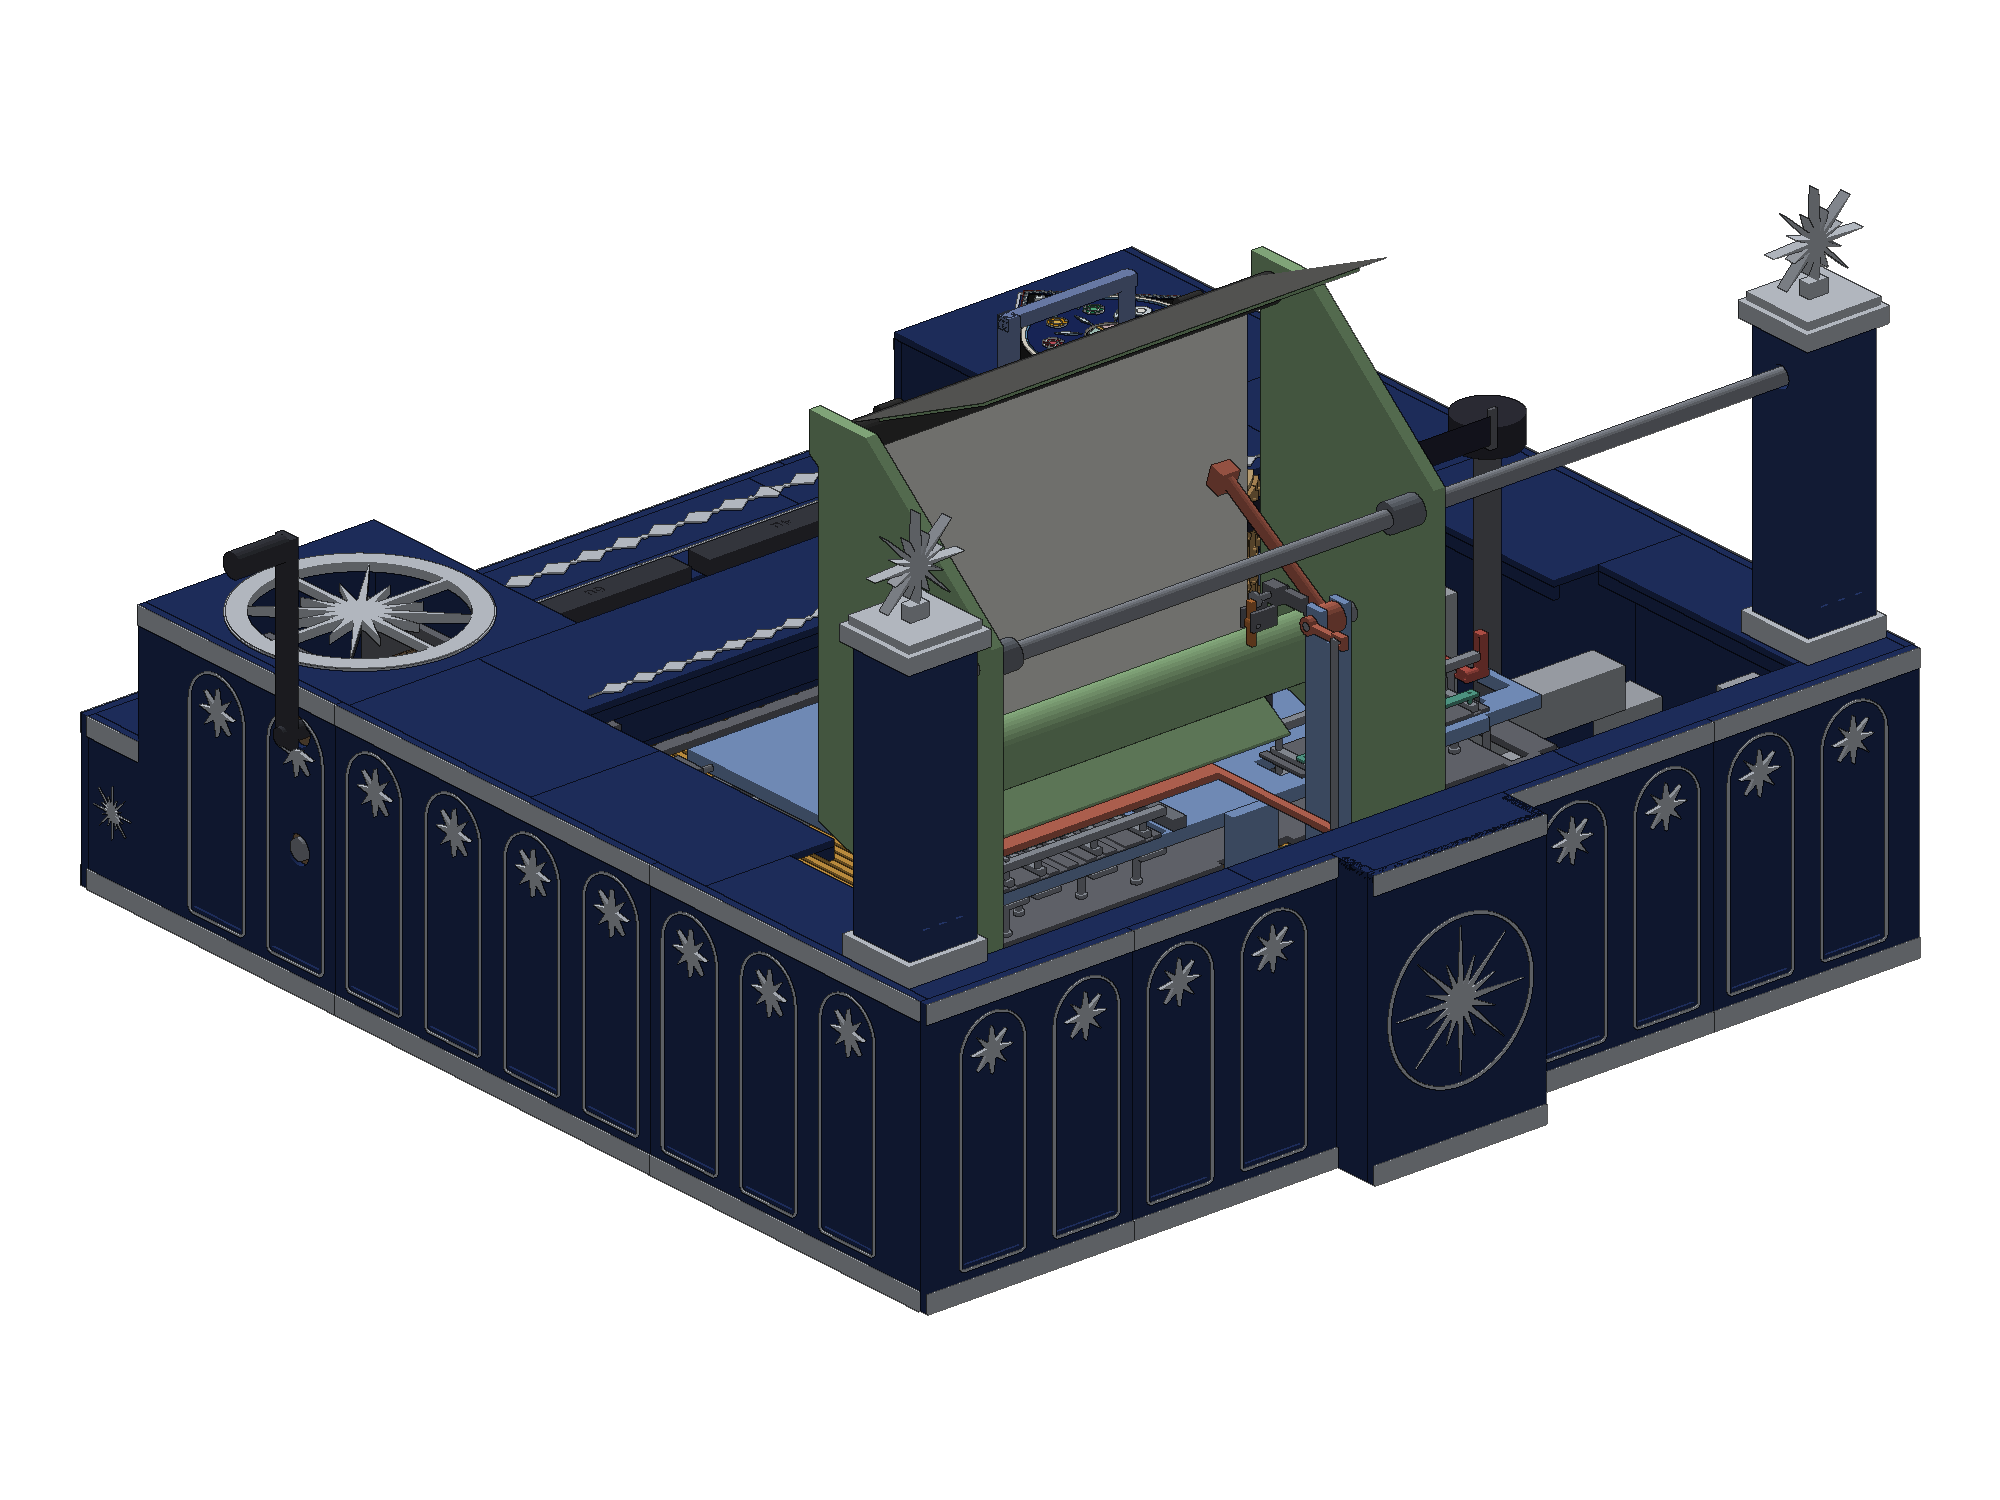
\includegraphics[width=\linewidth]{gen/model/renders/case_iso_back.png}
\caption{Вид сзади справа: эркер над спуском, ручка завода в нише правой стенки, пилястры над стойками каретки.}
\label{fig:caseback}
\end{figure}

%=====================================================================
\section{Спецификация узлов}
\label{sec:spec}

\begin{center}\small
\begin{tabularx}{\linewidth}{@{}>{\raggedright}p{50mm}r>{\raggedright\arraybackslash}X@{}}
\toprule
Узел & Кол-во & Замечание \\
\midrule
клавиши с рычагами & 44 & плюс служебные: регистр, два пробела, забой, «назад на литеру»; рычаги из двух частей \\
пластины признаков & 46 & по два яруса; винты без зазора R или О, N; у пробелов R и W; ход 16~мм; два поля \\
мерные рамки & 4 & R, W (пробелы), О, N; по два стальных прутка и две печатные боковины; четыре вертикальных направляющих 3~мм; сдвиг на 4,5~мм регистром \\
чтение кода & 1 & головка с тремя щупами на стойке U-рамы; кулачок и коромысло 11/33; 4 боуденовских троса; ползунки B и C на направляющих 2~мм; задвижка тяги W \\
освобождение каретки & 1 & клавиша-рычажок на передней раме, трос к собачке спуска, упор оболочки на задней стойке кронштейна \\
упоры полей & 2 + 1 & две защёлки на рейке каретки (шаг 6u), упор полей на кронштейне спуска \\
указатель точки печати & 1 & проволока 0,8~мм с красной бусиной на головке чтения \\
запоры холостого цикла & 2 & штыри Ø3 с головкой в направляющих на кронштейне коромысла чтения и на стойке молотка; рычажки 9/9~мм; 3 троса от повторителей О и W \\
толкатели и планки выбора & 13 + 7 & толкатель на столбец и по одному на рычаг пробела; планки разрядов позиции r1--r8 и ряда l1--l4 \\
коромысла & 2 & поворот (4 разряда) и подъём (3 разряда), ползуны и рычаги на кулисах, защёлки-пальцы; выходы — лента на шкив и вилка \\
челнок & 1 & печатное кольцо 106°, $R = 60$~мм; 11 литерных блоков по 8 литер в регулируемых гнёздах; 11 кодовых гребёнок на штифтах Ø2; скользит по валу, ведётся поводком за валом \\
пружинный двигатель & 1 & барабан Ø120, пружина 32$\times$0,8~мм, передача 1:53, завод ручкой через 1:3 \\
цикловой вал & 1 & защёлка цикла, регулятор, 6 кулачков: поворот, подъём, фиксаторы, молоток, лента, чтение \\
фиксаторы & 2 & колесо R 40 с 11 вырезами и клин; клин ряда в гребёнке на вилке, от той же тяги \\
молоток с пружиной & 1 & пружина кручения; рычаг взвода 19~мм, взвод 10--150°, спуск 160° \\
вибратор ленты & 1 & вилка из жести на ползуне, опускает ленту на 10~мм под строку \\
U-образная рама и ползун & 1 & плита Д16Т на MGN12; ход 9~мм; нулевой упор с регулировкой; пружина возврата \\
сектора памяти & 3 & B, C, W на соосных латунных трубках, повторители с роликами на ползунках B, C и балке рамки W; храповики с неравным шагом, собачки, сброс от трубки R; на B и C — ступени упоров отвода \\
упоры узла & 1 & нулевой упор с винтом и пружина возврата; щуп, синусный рычаг 15/15, каретка щупа, рычаг N; тяга от рамки О с пружиной и качалкой \\
переставной упор спуска & 1 & 4--16 зубьев; тяги 2~мм от троса щупа W и от рамки W (пробелы) синусным рычагом; задвижка до подачи \\
колесо спуска, шестерня, рейка & 1 & колесо 60 зубьев, шестерня $z = 10$, модуль 1,0106~мм: зуб колеса = 1\,u \\
каретка с пружинным двигателем & 1 & лист по схеме Хаммонда \\
блокировки & 3 & шариковая дорожка (одна клавиша), храповики полного хода на R и О, запорная гребёнка на время цикла \\
корпус & 1 & \mcasepieces~печатных деталей: стенки с нишами, деки, башни, лицо с надписью, щит с гербом, решётка-звезда, эркер, пилястры; на упорах к раме (\S\ref{sec:case}) \\
\bottomrule
\end{tabularx}
\end{center}

%=====================================================================
\section{Этапы макетирования}
\label{sec:stages}

\begin{enumerate}[label=Э\arabic*.]
  \item \textbf{Литеры и принтер.} Напечатать пробные штампы (ниже), оттиснуть через ленту или штемпельную подушку, проверить, что литеры и техты печатаются и читаются. Уточнить минимальные штрих и просвет своего принтера. Решает судьбу кегля и сопла до всякой механики.
  \item \textbf{Ползун, сектора и чтение.} Стенд на плите: ползун с нулевым упором, три сектора с фиксаторами, ползунки B и C, тяга упора спуска с задвижкой, головка чтения с тросами и макет кольца с двумя-тремя гребёнками, поворачиваемый вручную. Замерить ходы щупов по всем клеткам гребёнок, повторяемость упоров, трение тросов и силы.
  \item \textbf{Спуск.} Колесо спуска с переставным упором на 4--16 зубьев и каретка: проверить подачу по \S\,«Регулировка», п.~1.
  \item \textbf{Челнок.} Кольцо с блоками и гребёнками, шкив и колесо фиксатора, вилка подъёма, молоток, головка чтения; поворот и подъём вручную через коромысла: проверить фиксацию, оттиск, стойкость литер к удару и чтение в каждой позиции.
  \item \textbf{Двигатель и цикл.} Барабан с пружиной, передача, регулятор, цикловой вал с кулачками на стенде с челноком: замерить время оборота и расход завода на знак — это проверка главного расчёта \S\ref{sec:motor}.
  \item \textbf{Сборка.} Всё вместе, блокировки, программа испытаний; проверить с места пишущего, что строка видна (\S\ref{sec:vis}).
\end{enumerate}

\subsection{Э1: пробные штампы}

Штампы — плиты с зеркальным рельефом литер (рельеф 1,2~мм, основание 2,5~мм, поля 4~мм, треугольник в углу указывает верх). Печатаются лицом вверх, затем оттискиваются, как печать: прокатать валиком с краской или прижать к штемпельной подушке и с усилием приложить к бумаге. Оттиск показывает то же, что даст литера на челноке, кроме удара через ленту.

\begin{center}\small
\begin{tabularx}{\linewidth}{@{}lXrrr@{}}
\toprule
Файл & Что на штампе & em, мм & штрих, мм & размер, мм \\
\midrule
\tabinput{gen/tab_stamps.tex}
\bottomrule
\end{tabularx}
\end{center}

\begin{figure}[H]
\centering
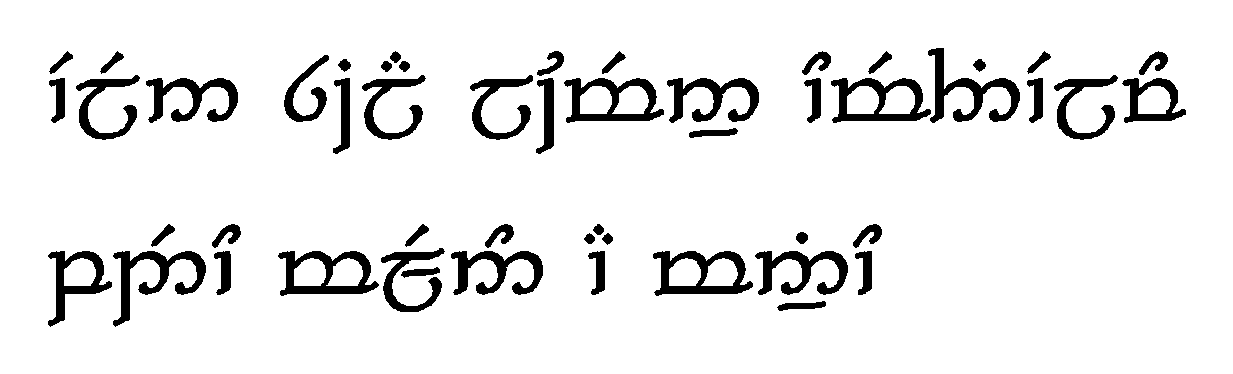
\includegraphics[width=0.75\linewidth]{stl/tpm2_em13_nozzle04_sample.png}
\caption{Штамп с образцами строк, em~=~1/3'', сопло 0,4~мм (вид на рельеф; на штампе он зеркальный).}
\label{fig:stamp}
\end{figure}

Что смотреть на оттиске: дуги не оторваны от ножек; знаки не слились с литерами; точки видны; соединения не залиты. Если всё в порядке, кегль и сопло подтверждены. Если сопло 0,25~мм, то выбор em~=~1/4'' уменьшает челнок, и его стоит предпочесть, но тогда шаг $k$ и ход пластины надо пересчитать (\code{tools/analysis\_fdm.py}).

%=====================================================================
\section{Риски и открытые вопросы}

\begingroup\sloppy
\begin{enumerate}[label=Р\arabic*.]
  \item \textbf{Расход завода — главный риск.} По расчёту завода хватает примерно на \mcharswind\ знаков; число зависит от КПД кулачков и трения, которые пока приняты. Если окажется меньше, — медленнее цикл, второй барабан или 6 рядов по 15 (\S\ref{sec:motor}).
  \item \textbf{Пружина.} В заведённой пружине около 150~Дж; барабан должен быть закрыт, крышки — на винтах, завод — с отпускной собачкой.
  \item \textbf{Износ литер.} Пластик под ударом через ленту мнётся и стирается быстрее металла. Блоки сменные; для стойкости — PETG или более твёрдые нити, а молоток с мягкой накладкой.
  \item \textbf{Ползучесть.} Пластиковые детали под постоянной нагрузкой (пружины, упоры) со временем текут. Все постоянные нагрузки идут через стальные оси и винты, пружины — на стальных зацепах.
  \item \textbf{Точность гребёнок.} Требование $\sigma \le 0{,}08$~мм к ходу щупа (\S\ref{sec:gaptol}) по оценке выполняется с запасом около 10\,\%; если печать или тросы окажутся хуже, ступень $k$ придётся увеличить до 1,2--1,5~мм/u (гребёнки глубже, головка ближе к валу). Настройки 44 пластин больше нет; есть три винта нуля.
  \item \textbf{Тросы.} Трение в оболочках и их усадка со временем сдвигают нуль канала; концы оболочек должны быть закреплены жёстко, а трасса — без крутых изгибов. Силы пружин щупов (0,45--0,6~Н) и нагрузок — допущения до стенда Э2.
  \item \textbf{Холостой цикл.} Запоры построены (\S\ref{sec:idle}); удар взводного рычага по запертому молотку гасит резиновая втулка штыря — её стойкость надо проверить на стенде.
  \item \textbf{Ползун под молотком.} Рама с молотком не должна перекашиваться при отводе и сдвигаться при ударе; нужна проверка жёсткости.
  \item \textbf{Скорость.} Около 2,5 знака в секунду (150 в минуту); дальние литеры — около двух. Быстрее — только ценой завода (\S\ref{sec:motor}).
  \item \textbf{Заправка листа.} Молоток за листом — заправка неудобнее, чем на рычажной машинке.
  \item \textbf{Память на одну литеру.} Знаки ставятся только к последней букве.
  \item \textbf{Частоты рядов} оценены по именам и коротким фразам, а не по связному тексту; если в реальном тексте частоты окажутся другими, ряды челнока можно переставить, переставив выступы l1 и l2 на рычагах, литерные блоки и гребёнки, — механика не меняется.
  \item \textbf{Неравный шаг храповиков памяти} задан расчётом повторителя; ошибка радиуса ролика или высоты балки сдвигает все зубья сразу, поэтому повторитель нужно выставлять по контрольному набору (Регулировка).
\end{enumerate}
\endgroup

\subsection*{Что нужно для перехода к рабочим чертежам}

\begin{itemize}
  \item стенд Э5: время цикла и расход завода на знак (с ред. 0.10 — вместе с работой щупов);
  \item стенд Э2: ходы щупов по клеткам гребёнок и трение тросов;
  \item результат этапа Э1: оттиски штампов и уточнённые минимальные штрих и просвет принтера;
  \item замеры стенда Э2: силы пружин, трение, повторяемость упоров — они заменят допущения \S\ref{sec:forces} и \S\ref{sec:prec};
  \item подбор пружин спуска, забоя и памяти M по стенду Э2 (\S\ref{sec:back});
  \end{itemize}

%=====================================================================
\appendix
\section{Сборочные листы}
\label{app:asm}

Для каждой группы — разнесённый вид: детали отодвинуты от центра группы, сохраняя порядок. В кружках — номера печатных деталей (те, что вдавлены в детали и стоят в начале имён файлов STL); серым — покупные и нарезаемые детали (перечень — \S\ref{sec:model}). Ниже — таблица номеров.

\IfFileExists{gen/model/assembly.json}{}{}
\foreach \g in {frame,keys,levers,plates,bails,sectors,select,uframe,shuttle,carriage,esc,ribbon,drive,hammer,case}{%
\IfFileExists{gen/model/renders/asm_\g.png}{\begin{figure}[H]\centering\includegraphics[width=\linewidth]{gen/model/renders/asm_\g.png}\end{figure}}{}}

{\footnotesize\renewcommand\arraystretch{0.9}
\begin{longtable}{@{}rp{70mm}rp{55mm}l@{}}
\toprule
№ & первая деталь & шт. & группа & номер \\
\midrule
\endhead
\tabinput{gen/tab_part_numbers.tex}
\bottomrule
\end{longtable}}

\section{Коды литер}

$w$ — подача, $a$ — от края клетки до оси техты (для справки), $b$ — отвод для надстрочных знаков, $d$ — смещение нижней оси, $c = b - d$ — отвод для подстрочных. Всё в $u$.

{\small\setlength\tgem{5.5mm}
\begin{longtable}{@{}cllrrrrr@{}}
\toprule
& Литера & U+ & $w$ & $a$ & $b$ & $d$ & $c$ \\
\midrule\endhead
\tabinput{gen/tab_codes.tex}
\bottomrule
\end{longtable}}

\section{Кодовые гребёнки}
\label{app:combs}
\label{app:plates}

Для каждой продвигающей литеры: позиция челнока (столбец клавиатуры) и ряд, литера, ширина $w$, значения $b$ и $c$ и радиусы торцов её зубцов W ($w - 4$), B и C от оси челнока; последняя колонка — сошлась ли проверка чтения на модели (\S\ref{sec:read}). Клетки мёртвых знаков и пустые клетки зубцов не имеют. До редакции 0.9.3 здесь стояла таблица зазоров кодовых пластин; пластины теперь несут только R, О и N без зазора.

{\small\setlength\tgem{5mm}
\begin{longtable}{@{}rrcl rrr rrr c@{}}
\toprule
Поз. & Ряд & & Литера & $w$ & $b$ & $c$ & $r_W$ & $r_B$ & $r_C$ & чтение \\
\midrule\endhead
\tabinput{gen/tab_combs.tex}
\bottomrule
\end{longtable}}

\section{Отклонённые варианты}

\begin{description}[style=nextline,leftmargin=0pt]
  \item[Рычажная машинка с салазками знаков (ред. 0.1).] Проще по приводу, но выравнивание держится по 44 рычагам и двум салазкам (по Монте-Карло — почти вдвое хуже посадка знаков), сила удара зависит от пальца, раскладка ограничена.
  \item[Кегль 1/6'' (ред. 0.2--0.3).] Лёгкий челнок, но на FDM не печатается: волосяные штрихи Alcarin (около 0,3~мм) уже сопла, литеры пропадают целиком (\S\ref{sec:glyphs}).
  \item[Останов челнока на штифте (ред. 0.5).] Удар об упор на каждом знаке и энергия, которую нужно гасить; заменён кулачковым приводом с фиксатором.
  \item[Челнок 4$\times$22 с пружинным двигателем.] Энергии на знак втрое больше, чем при 8$\times$11; завода хватало бы на 300--400 знаков.
  \item[Литеры, собранные из ножек и дуг.] Меньше разных деталей, но больше риск ошибочного контура на стыке; принят цельный рисунок.
  \item[Без нижней оси.] Ошибка подстрочного знака — $d$: 0,26~мм у основных тенгв, 0,8~мм у hyarmen.
  \item[Без «назад на литеру».] Исправление — до 16 ударов забоя.
  \item[Код под клавишами (ред. 0.4--0.9.3).] Выступы W, B и C на кодовых пластинах с зазорами, выставленными щупом, и мерные рамки. Точно, но шрифт прибит к пластинам: другой шрифт — это перестановка до 216 винтов (по три на каждую из 72 продвигающих литер; \S\ref{sec:read}).
  \item[Сменная кассета пластин.] Пластины снимаются с рычагов, на каждый шрифт — свой комплект, выставленный на калибре. Механика прежняя, но диапазоны кода по-прежнему заданы ходом клавиши, а 46 пластин на шрифт — много.
  \item[Двоичный код на челноке.] Штырьки «есть/нет» вместо глубины зубца не боятся допусков печати, но требуют 12 щупов и трёх коромысел-сумматоров; отклонён ради простоты.
  \item[Гребёнки выше пояса, головка над валом.] Не надо переставлять поводок, но гребёнки торчат над челноком на 15~мм и в покое, по оценке, закрывали бы последние 40~мм строки; чтобы этого не было, челнок пришлось бы опускать глубже, а это энергия на каждом знаке.
  \item[Тяжёлые приёмники.] Щуп W, тянущий рамку W целиком (около 95~г стальных прутков), не успевает за 25° цикла без пружины в 3--4~Н; поэтому W тянет только лёгкую тягу Y упора спуска, а B и C — ползунки вместо рамок.
  \item[Моноширинная переделка.] Простая и точная, но без пропорциональных ширин и требует донорской машинки.
\end{description}

\section*{Источники}
\begin{itemize}\small
  \item G.\,C.~Mares. History of the Typewriter. London, 1909, с.~143 — \url{https://tekniskkulturarv.dk/book/21c52e37-c94c-4fd7-8f2f-df7031f6b69b?page=151}.
  \item The Virtual Typewriter Museum: Hammond~1 (башенка со штифтами) — \url{https://typewritermuseum.org/collection/brands/index.php?machine=hammond1&cat=ks}.
  \item KBD.news: Hammond~2 (челнок 118°, три ряда, подъём наковальни) — \url{https://kbd.news/Hammond-2-typewriter-2140.html}.
  \item Mind Machine: Hammond Typewriter (взвод молотка возвратом каретки; скорость) — \url{https://mindmachine.co.uk/products/04_Manuf_Hammond_01.html}.
  \item Antique Typewriters: Hammond~1 — \url{https://antiquetypewriters.com/typewriter/hammond-1-typewriter}.
  \item Collectors Weekly: Beautiful Machine: 1881 Hammond — \url{https://collectorsweekly.com/articles/?p=16805}.
  \item US~780102 (Хаммонд: молоток, челнок, U-образная рама) — \url{https://patents.google.com/patent/US780102A/en}.
  \item Collectors Weekly: 1881 Hammond (кассета бумаги под валиком, молоток за листом) — \url{https://www.collectorsweekly.com/articles/beautiful-machine-1881-hammond-typewriter/}.
  \item US~2581200 (Varityper) — \url{https://patents.google.com/patent/US2581200}.
  \item US~2904159 (пропорциональный спуск) — \url{https://patents.google.com/patent/US2904159A/en}.
  \item IBM Selectric Composer (единицы 1/72, 1/84, 1/96'') — \url{https://ibmselectric-typewriter.blogspot.com/2011/12/selectric-composer.html}.
  \item Firgelli: Beater Bar (люфт рычага в прорези, отношение клавишного рычага) — \url{https://www.firgelliauto.com/blogs/mechanisms/beater-bar-typewriter}.
  \item HP Museum: Mechanical adders (комптометр) — \url{https://hpmuseum.org/adddir.htm}.
  \item Остальные источники (Alcarin Tengwar, раскладка Смита, IBM Executive) — в документе ТПМ-1.
\end{itemize}

\end{document}
